\documentclass[10pt,a4paper]{article}

% =============================================================================
% SPRINGER NATURE / JOURNAL OF BIG DATA (FRAMEWORK PAPER SUBMISSION FORMAT)
% =============================================================================
\usepackage[utf8]{inputenc}
\usepackage[T1]{fontenc}
\usepackage{mathptmx}
\usepackage[scaled=0.90]{helvet}
\usepackage{courier}
\usepackage[a4paper,top=14.2mm,bottom=14.2mm,left=15.0mm,right=15.0mm]{geometry}
\usepackage{amsmath,amsfonts,amssymb}
% Fix mathptmx calligraphic font rendering (\mathcal{M}, \mathcal{B}, \mathcal{R}, \mathcal{E})
\DeclareMathAlphabet{\mathcal}{OMS}{cmsy}{m}{n}
\usepackage{graphicx}
\usepackage{booktabs}
\usepackage{multirow}
\usepackage{array}
\usepackage{xcolor}
\usepackage{fancyhdr}
\usepackage{lastpage}
\usepackage{titlesec}
\usepackage{enumitem}
\usepackage[labelfont={bf,sf,small},textfont={sf,small},labelsep=period]{caption}
\usepackage[switch, modulo]{lineno}
\usepackage[colorlinks=true,linkcolor=blue!70!black,citecolor=blue!70!black,urlcolor=blue!70!black]{hyperref}

\definecolor{springerblue}{RGB}{0, 102, 153}

% Clean submission running header without placeholder tokens
\pagestyle{fancy}
\fancyhf{}
\fancyhead[L]{\footnotesize\sffamily Noiumkar \quad \textit{Journal of Big Data} --- Research Article Submission}
\fancyhead[R]{\footnotesize\sffamily Page \thepage\ of \pageref*{LastPage}}
\renewcommand{\headrulewidth}{0.4pt}

\titleformat{\section}{\large\sffamily\bfseries\color{springerblue}}{\thesection}{0.6em}{}
\titleformat{\subsection}{\normalsize\sffamily\bfseries}{\thesubsection}{0.6em}{}
\titleformat{\subsubsection}{\normalsize\sffamily\bfseries\itshape}{\thesubsubsection}{0.5em}{}
\setlength{\parindent}{0pt}
\AtBeginDocument{\setlength{\abovedisplayskip}{3.2pt plus 1.0pt minus 1.0pt}\setlength{\belowdisplayskip}{3.2pt plus 1.0pt minus 1.0pt}}

% --- Float Queue & Placement Tuning (Prevent Tables Drifting After References) ---
\renewcommand{\topfraction}{0.95}
\renewcommand{\bottomfraction}{0.95}
\renewcommand{\textfraction}{0.05}
\renewcommand{\floatpagefraction}{0.85}
\setcounter{topnumber}{5}
\setcounter{bottomnumber}{5}
\setcounter{totalnumber}{10}
\makeatletter\g@addto@macro{\UrlBreaks}{\UrlOrds\do\-\do\_\do\/\do\.\do\0\do\1\do\2\do\3\do\4\do\5\do\6\do\7\do\8\do\9}\makeatother
\Urlmuskip=0mu plus 2mu\relax
\emergencystretch=1.5em
\newsavebox{\asttblbox}
\newsavebox{\asttblboxB}
\newenvironment{fitasttable}{%
  \begin{lrbox}{\asttblbox}%
}{%
  \end{lrbox}%
  \sbox{\asttblboxB}{%
    \ifdim\wd\asttblbox>0.96\textwidth
      \resizebox{0.96\textwidth}{!}{\usebox{\asttblbox}}%
    \else
      \usebox{\asttblbox}%
    \fi
  }%
  \ifdim\ht\asttblboxB>0.72\textheight
    \resizebox{!}{0.72\textheight}{\usebox{\asttblboxB}}%
  \else
    \usebox{\asttblboxB}%
  \fi
}

\emergencystretch=1.4em
\tolerance=800
% --- SPRINGER / BMC CLEAN HEADING, LIST & FLOAT SPACING ---
\makeatletter
\renewcommand\section{\@startsection{section}{1}{\z@}%
  {-9.5pt \@plus -2pt \@minus -1.5pt}%
  {3.5pt \@plus 1pt}%
  {\normalfont\large\bfseries}}
\renewcommand\subsection{\@startsection{subsection}{2}{\z@}%
  {-7.5pt \@plus -2pt \@minus -1pt}%
  {2.8pt \@plus 1pt}%
  {\normalfont\normalsize\bfseries}}
\renewcommand\subsubsection{\@startsection{subsubsection}{3}{\z@}%
  {-6pt \@plus -1.5pt \@minus -1pt}%
  {2.0pt \@plus 0.8pt}%
  {\normalfont\normalsize\bfseries}}
\makeatother
\linespread{0.852}\selectfont
\setlength{\parskip}{0.3pt plus 0.1pt minus 0.1pt}
\setlength{\textfloatsep}{2.8pt plus 1.0pt minus 1.0pt}
\setlength{\floatsep}{2.5pt plus 1.0pt minus 1.0pt}
\setlength{\intextsep}{2.8pt plus 1.0pt minus 1.0pt}
\setlength{\abovecaptionskip}{2.0pt plus 0.8pt minus 0.8pt}
\setlength{\belowcaptionskip}{1.0pt plus 0.8pt minus 0.8pt}
\setlist{topsep=0.5pt,itemsep=0.2pt,parsep=0.1pt}
\begin{document}
\linenumbers
\expandafter\def\expandafter\UrlBreaks\expandafter{\UrlBreaks\do\-\do\_\do\/\do\.\do\0\do\1\do\2\do\3\do\4\do\5\do\6\do\7\do\8\do\9\do\a\do\b\do\c\do\d\do\e\do\f}

% =============================================================================
% SPRINGEROPEN / JOURNAL OF BIG DATA FRONTMATTER (FRAMEWORK PAPER FRAMING)
% =============================================================================
{\footnotesize\sffamily\color{springerblue}\textbf{RESEARCH ARTICLE} \hfill \textbf{Journal of Big Data (SpringerOpen)}}\\[0.8em]

{\raggedright\LARGE\sffamily\bfseries AST-Route: An AST-Aware Multi-Objective Query Routing and Cost-Prediction Framework Across Serverless Cloud, \mbox{Vectorized} CPU (C++/Rust), and GPU-Accelerated OLAP Engines}\\[0.9em]

{\large\textbf{Preecha Noiumkar\textsuperscript{1,*}}}\\[4pt]
\textsuperscript{1}Department of Information Technology, Faculty of Informatics, Mahasarakham University, Kham Riang, \mbox{Kantharawichai}, Maha Sarakham 44150, Thailand.\\
\textsuperscript{*}Correspondence: Preecha Noiumkar (\href{mailto:preecha.n@msu.ac.th}{preecha.n@msu.ac.th})\\[0.8em]

\noindent\rule{\textwidth}{0.8pt}
\begin{quote}
\small\sffamily
\textbf{\color{springerblue}Abstract}\\[0.3em]
\textbf{Background:} Hybrid analytical engines spanning cloud SQL, C++/Rust CPUs, and CUDA GPUs exhibit severe query-dependent crossover where static engine selection suffers high tail regret from PCIe transfers and memory ceilings.

\textbf{Objective \& Thesis:} We test one central thesis: pre-execution SQL abstract syntax tree (AST) features paired with zone-map selectivity and conformal guards can match static GPU mean latency while cutting 95th-percentile (P95) tail regret by over $2\times$.

\textbf{Methods:} Across 400 queries, 10 suites, 4 nodes, and scales up to 100 GB, \textbf{AST-Route} uses a 9D vector and gradient-boosted trees with Mondrian conformal bounds and co-equal 8\%/12\% PCIe guards.

\textbf{Results:} Under 25-seed cross-validation ($N=75$, 1 GB), AST-Route achieves 56.00\%/57.33\% exact Top-1 accuracy (74.67\% Pure-SQL), 55.37--54.92 ms net latency ($1.50\times$ vs.\ Polars, $p_{\text{Holm}}=0.0011$), and $2.17\text{--}2.25\times$ lower P95 regret than Always GPU (118.40\%/114.11\% vs.\ 257.31\%, $p_{\text{tpl}}=0.0074$). With \texttt{NVIDIA RAPIDS cudf-polars} on TPC-H Q1--Q22 (1/10 GB), it reaches 95.45\% exact Top-1 and 0.00\% P95 regret.

\textbf{Conclusion:} Conformal AST routing delivers tail-safe cross-engine SQL dispatch.

\noindent\textbf{Keywords:} Cross-engine query routing; Tail-risk control; Conformal prediction; Heterogeneous OLAP systems; Apache Arrow and GPU analytics; Multi-objective cost modeling
\end{quote}

\section{Introduction}
Modern enterprise analytics increasingly operate over heterogeneous, polyglot data infrastructures spanning four distinct computing paradigms: elastic serverless cloud data warehouses such as Google BigQuery \cite{melnik2010dremel, melnik2020dremel, lounissi2025funda}, in-process C++ vectorized analytical database systems such as DuckDB \cite{raasveldt2019duckdb, kuiper2024duckdb_ooc}, Rust-based Apache Arrow streaming query engines such as Polars and Apache DataFusion \cite{lamb2024datafusion}, and SIMT GPU-accelerated relational engines \cite{chrysogelos2019hetexchange, shanbhag2020crystal, bress2013hype}, alongside distributed multi-node systems like ClickHouse \cite{schulze2024clickhouse} and Trino \cite{sethi2019presto}. While cloud-native disaggregated storage-compute architectures provide massive horizontal slot concurrency for petabyte-scale workloads \cite{shojaee2024serverless, abdalla2022bigdata}, they introduce non-trivial stateless scheduling and distributed shuffle overheads on moderate-scale datasets \cite{begoli2018calcite, garcia2008database, lounissi2025funda}. Concurrently, modern local hardware presents an intricate architectural trade-off between CPU SIMD vectorization over Apache Arrow memory buffers and discrete GPU offloading across the PCIe interconnect \cite{milicevic2024dlquery, root2019mapd, kim2022blazingsql}.

Because each execution paradigm exhibits fundamentally different algorithmic strengths and memory-hierarchy bottlenecks across the discrete scale factors defined by the Transaction Processing Performance Council ($\text{SF} \in \{1, 10, 30, 100\text{ GB}\}$ in the TPC-H specification \cite{tpc2022tpch, boncz2014tpch, dreseler2020quantifying}), committing an entire analytical workload to any single static engine results in severe performance regret, excessive energy consumption, out-of-core spilling penalties, or unnecessary cloud FinOps expenditure. Designing an automated, pre-execution query routing framework capable of dynamically dispatching SQL queries to their optimal execution backend requires overcoming three critical research gaps in the existing literature \cite{ahmed2020hibench, oneil2009ssb, leis2015job}:
\begin{itemize}[leftmargin=1.5em,itemsep=2pt]
    \item \textbf{Research Gap 1 (Limitations of Single-Engine Learned Optimizers, Cloud Predictors, and Plan-Dependent Polystore Routers):} Existing learned query optimizers such as Neo \cite{marcus2019neo} and Bao \cite{marcus2021bao} steer physical operator plans \emph{within} a single database engine, Zero-Shot Cost Models \cite{hilprecht2022zeroshot} require physical execution plan graphs, cloud stage predictors \cite{ganapathi2009predicting, nathan2024stage} estimate runtimes within a single cloud warehouse, and cross-platform/polystore optimizers such as BigDAWG \cite{tan2023stage} and RHEEM / Apache Wayang \cite{gupta2023adaptive} require compiling query sub-plans into platform-specific operator DAGs using calibrated point-estimate cost functions without modeling Apache Arrow vs.\ PCIe GPU transfer thresholds or distribution-free conformal tail-risk bounds. A lightweight pre-execution framework that extracts static Abstract Syntax Tree (AST) features and zone-map selectivity directly from raw SQL to route queries across C++ DBMS, Rust Arrow, CUDA GPU, and serverless cloud paradigms remains underdeveloped.
    \item \textbf{Research Gap 2 (Unmodeled PCIe Crossover Thresholds, Memory Walls, and Device-Level Energy Costs):} Prior GPU database studies \cite{shanbhag2020crystal, root2019mapd, kim2022blazingsql} predominantly report warm in-VRAM kernel speedups at fixed small scale factors ($\text{SF}=1\text{ GB}$) while omitting cold-start PCIe Host-to-Device (H2D) transfer overheads, chunked PCIe streaming when datasets exceed device VRAM ($\text{SF}=10, 30, \text{and } 100\text{ GB}$), out-of-core host RAM disk spilling \cite{kuiper2024duckdb_ooc}, and hardware energy efficiency ($\text{Joules}$ and $\text{MB/J}$).
    \item \textbf{Research Gap 3 (Confounded Complexity, Data Leakage, and Lack of Nested Cross-Workload Validation):} Traditional OLAP evaluations \cite{ahmed2020hibench, abdalla2022bigdata} rely on unstratified query sets where structural operator depth, storage layout (row-store vs. Parquet vs. Arrow), and predicate selectivity are confounded, and where random train-test splits across variations of the same query template induce severe data leakage without testing generalization to unseen seeds, join-crossing skew correlations \cite{boncz2017jcch}, or nested cross-validation on standard TPC-H Q1--Q22 choke-point workloads \cite{boncz2014tpch, dreseler2020quantifying}.
\end{itemize}

\par\vspace{7pt plus 2pt minus 1pt}\noindent\textbf{Bridging Memory-Wall Big Data Orchestration, Crossover Profiling, and Risk-Aware Routing.}
In modern hybrid analytics, "Big Data" scale is defined not solely by petabyte cluster volume, but by the ratio of query working-set footprint to local memory-hierarchy capacity ($\mathcal{B}_{\text{work}}(q)/M_{\text{cap}} \in [0.05\times, 6.25\times]$, spanning in-VRAM execution at $\text{SF}=1\text{ GB}$, out-of-VRAM PCIe chunked streaming at $\text{SF}=10\text{--}30\text{ GB}$, and heavy out-of-core NVMe spilling vs.\ elastic serverless cloud offloading at $\text{SF}=100\text{ GB}$ [$866.1\text{M}$ rows]). Designing a reliable cross-paradigm dispatcher across this continuum requires resolving a fundamental systems tension: static single-engine policies suffer severe performance cliffs across heterogeneous operators, yet naive point-estimate cost minimization (unconstrained $\arg\min$ over predicted latency $\hat{T}_e(q)$) triggers costly tail-latency spikes whenever prediction intervals overlap near CPU--GPU PCIe crossover boundaries or device memory ceilings. Rather than treating hardware benchmarking and learned routing in isolation, this study grounds an interpretable, zero-execution routing architecture directly in controlled factorial crossover telemetry within a well-defined hardware envelope ($4.0\text{ GB}$ PCIe Gen4 discrete GPU, $16\text{ GB}$ host DRAM with $9.0\text{ GB}$ DBMS cap, cross-checked on 22-thread \texttt{x86\_64} and Apple M1 \texttt{ARM64} nodes). Crucially, decoupling the pre-execution structural/volume representation ($\mathbf{x}_q \in \mathbb{R}^9$, extended to $\mathbf{x}_q^{\text{scale}}\in\mathbb{R}^{10}$) from the downstream decision policy exposes an explicit operational trade-off between \emph{unconstrained mean-latency minimization} and \emph{tail-safe SLA protection} (governed via calibrated conformal prediction intervals and resource-constrained Pareto dispatch). Detailed metrics, negative results, and scope boundaries are consolidated in Table~\ref{tab:key_findings_glance}, organized around three concise contributions:
\begin{enumerate}[leftmargin=1.5em,itemsep=3pt]
    \item \textbf{Claim 1 --- Cross-Paradigm Crossover Characterization Across a Four-Category Epistemic SQL Corpus ($N_{\text{total}}=400$):} Using six execution engines across four paradigms ($\mathcal{E}_{\text{All-6}}$) as a controlled cross-paradigm testbed across $\text{SF}\in\{1,10,30,100\}\text{ GB}$ and $\mathbf{400}$ SQL queries partitioned into four transparent epistemic categories ($\mathbf{75}$ \emph{Core Development}, $\mathbf{55}$ \emph{Diagnostic Standard} [$22$ Official TPC-H $+$ $33$ IMDB JOB], $\mathbf{115}$ \emph{Author-Derived Zero-Shot}, and $\mathbf{155}$ \emph{Held-Out Third-Party Standard Benchmarks} [$99$ Official TPC-DS $+$ $43$ ClickBench $+$ $13$ SSB, not used in training or feature design]; Section~\ref{sec:layer1_ast_taxonomy} and Additional File~1, Table~S18), we show that no single engine dominates all operators. DuckDB is the fastest single engine overall on official TPC-H Q1--Q22 ($22.82\text{ ms}$ vs.\ $42.79\text{ ms}$ Polars, $1.88\times$) due to correlated subqueries (Q16--Q22), whereas Rust Arrow engines (Polars, DataFusion) lead low-arithmetic scans (Tier~L1) and CUDA GPUs dominate compute-heavy joins, windows, and array unnests (L2--L5) once post-pushdown volume amortizes PCIe transfer ($\Phi_{\text{PCIe}}$).
    \item \textbf{Claim 2 --- Multi-Objective Pareto Routing (Policies P1--P4) and Tail-Risk Control via a Minimalist 2/3-Engine Subset (Co-Equal $8\%$ Nested-CV and $12\%$ Default Guards):} Under an evaluation protocol \emph{pre-specified in repository, not externally registered} ($K=25$ seed clusters at $\text{SF}=1\text{ GB}$, serialized frozen model SHA-256 \texttt{f0e5f17c...} distinct from telemetry CSV SHA-256 \texttt{89b1ec64...}), we report the inner 24-seed \textbf{Nested-CV Guard ($\hat{\tau}_{\text{guard}}^{(-k)}=8\%$)} and the \textbf{Default Guard ($\tau_{\text{guard}}=12\%$)} on \textbf{strictly co-equal footing}. Under Speed-First Policy~P1 ($\alpha=1,\beta=0,\gamma=0$), both co-equal guards match Always GPU ($56.96\text{ ms}$) in mean latency without claiming raw mean superiority ($p_{\text{seed}}=0.184$): the co-equal $8\%$ Nested-CV Guard ($\mathbf{55.37\text{ ms}}$) passes two-sided $\pm 5.0\text{ ms}$ TOST ($\mathbf{p_{\text{TOST}}=0.0442 < 0.05}$), whereas the co-equal $12\%$ Default Guard ($\mathbf{54.92\text{ ms}}$) passes one-sided non-inferiority ($p_{\text{non-inf}}=0.00067$) and $\pm 6.0\text{ ms}$ TOST ($p=0.0241$) \textbf{but does not pass $\pm 5.0\text{ ms}$ TOST ($p_{\text{TOST}}=0.0688 > 0.05$)} while beating static CPUs by $1.49\times\text{--}3.35\times$ ($p_{\text{Holm,seed}}\le 0.0171$, Nadeau--Bengio $p_{\text{NB}}\le 0.0086$), compressing P95 tail regret by $\mathbf{2.17\times}$ ($257.31\% \rightarrow \mathbf{118.40\%}$ at $8\%$, $p_{\text{Holm,seed}}=0.0230, p_{\text{NB}}=0.0118$; $\mathbf{2.25\times}$ to $\mathbf{114.11\%}$ at $12\%$), cutting $\text{CVaR}_{10\%}$ by $\mathbf{2.21\times}$ ($349.40\% \rightarrow \mathbf{158.42\%}$), and lowering $\text{AURC}$ by $\mathbf{-39.9\%}$ ($46.82\% \rightarrow 28.14\%$). Under hierarchical $G_{\text{core}}=10$ template-family cluster bootstrap and Rademacher wild cluster bootstrap ($10{,}000$ iterations), AST-Route's P95 and $\text{CVaR}_{10\%}$ tail-regret reductions remain statistically significant against both \textbf{Always GPU} ($\Delta\mathcal{R}_{\text{P95}}=-138.91\text{ pp}$ [$p_{\text{tpl}}=0.0074$] for $8\%$ and $-143.20\text{ pp}$ [$p_{\text{tpl}}=0.0061$] for $12\%$) and the strongest unguarded baseline, \textbf{Ridge Linear Regression} ($\Delta\mathcal{R}_{\text{P95}}=-82.70\text{ pp}$ [$p_{\text{tpl}}=0.0438$], $\Delta\text{CVaR}_{10\%}=-244.42\text{ pp}$). To uphold strict measurement rigor, we withdraw TDP-estimated host CPU package energy from our headline claims (deferring exploratory Host+Device system estimates to Additional File~1, Table~S23) and anchor primary energy claims strictly on \textbf{direct 50~Hz hardware-sensor \texttt{pynvml} GPU telemetry} ($0.644\text{ J/q}$ on Node~1 RTX~2050, $0.668\text{ J/q}$ on \texttt{CuPy v14.2.0}, $0.875\text{ J/q}$ on Node~4 Cloud-Hosted Server NVIDIA Tesla~T4) and \textbf{1,500-run cloud hardware-register telemetry} (Intel RAPL, AMD SMU, and NVML). Across Policies~P1--P4 (verified as \emph{Pareto-efficient among the evaluated policy configurations} across $500$ Dirichlet simplex samples with $\text{DSR}=\mathbf{0.0\%}$), Energy-Aware \textbf{Policy~P2 $(0.1,0.8,0.1)$} achieves $\mathcal{R}_E=4.82\%$, Cost-First \textbf{Policy~P3 $(0.2,0.1,0.7)$} enforces $\mathbf{\$0.00/1\text{M}}$ cloud spend at $\text{SF}=100\text{ GB}$ (saving $\mathbf{\$507.06/1\text{M}}$, $\mathcal{R}_C=0.0\%$), and Balanced \textbf{Policy~P4 $(0.5,0.3,0.2)$} achieves the maximum 3D Pareto Hypervolume ($\mathbf{\text{HV}=0.9210}$ at $\text{SF}=1\text{ GB}$, $\mathbf{0.9340}$ at $\text{SF}=100\text{ GB}$). Practically, a \textbf{Minimalist 2-Engine Subset ($\mathcal{E}_{\text{Min-2}}=\{\text{Polars},\text{GPU}\}$: $\mathbf{55.28\text{ ms}}$)} captures $\mathbf{98.7\%}$ of the 6-engine gain ($\mathcal{E}_{\text{Prod-3}}=\{\text{DuckDB},\text{Polars},\text{GPU}\}$: $\mathbf{55.07\text{ ms}}$ captures $\mathbf{99.5\%}$ with $0.0\text{ MB}$ storage duplication; Pure-SQL $\mathcal{E}_{\text{SQL-5}}: \mathbf{69.12\text{ ms}}$ captures $48.5\%$).
    \item \textbf{Claim 3 --- Operational Scope Boundaries, Multi-Scale TPC-DS Generalization ($\text{SF}=0.02 / 1 / 10\text{ GB}$), and Explicit Negative Results:} Validated via 100\% physical execution across four hardware nodes (Node~1 \texttt{x86\_64}+RTX~2050 $4.0\text{ GB}$ VRAM across pinned $5.69\text{ GB/s}$ vs.\ unpinned $3.36\text{ GB/s}$ PCIe DMA, Node~2 22T \texttt{x86\_64}, Node~3 Apple M1 \texttt{ARM64}, and Node~4 Cloud-Hosted Server NVIDIA Tesla~T4 $15.0\text{ GB}$ GDDR6 VRAM [\texttt{G2}, CUDA~13.0, single-pass $23.02\text{ ms}$ cold at $\text{SF}=1\text{ GB}$ and $461.71\text{ ms}$ at $\text{SF}=10\text{ GB}$, SHA-256 \texttt{32834476...}]), independent third-party \textbf{\texttt{NVIDIA RAPIDS cudf-polars 26.10.2} (\texttt{libcudf-cu12==26.10.2}, \texttt{cudf-streaming-cu12==26.10.2})} alongside external \texttt{CuPy v14.2.0} CUDA~12 and \texttt{Polars-Arrow-CuPy} ($\text{EX}=1.000$, $\mathbf{100.0\%}$ routing decision agreement, $\rho=0.9999$; on Official TPC-H Q1--Q22, \textbf{AST-Route + \texttt{RAPIDS cudf-polars}} achieves $\mathbf{95.45\%}$ \textbf{Exact Top-1} and $\mathbf{0.00\%}$ \textbf{P95 regret} at both $\text{SF}=1\text{ GB}$ [$\mathbf{70.59\text{ ms}}$ exec vs.\ $137.86\text{ ms}$ static \texttt{cudf-polars} and $77.17\text{ ms}$ Polars CPU] and $\text{SF}=10\text{ GB}$ [$\mathbf{1{,}524.39\text{ ms}}$ exec vs.\ $2{,}012.58\text{ ms}$ out-of-core \texttt{cudf-streaming-cu12}], while compressing Core 75Q P95 regret by $\mathbf{16.50\times}$ [$2{,}562.35\%\rightarrow 155.29\%$]), and $C=1\text{--}64$ concurrency ($154.44\text{ QPS}$ peak at $C=32$), AST-Route generalizes zero-shot across TPC-DS scales: on the held-out \textbf{99-query unmodified Official TPC-DS benchmark ($\text{SF}=0.02$, $605{,}865$ rows, $0$ training labels)}, it achieves $100\%$ ($99/99$) completion at $\mathbf{30.49\text{ ms}}$ ($\mathbf{64.65\%}$ \textbf{exact Top-1} on $\mathcal{E}_{\text{All-6}}$, $\mathbf{84.85\%}$ on $\mathcal{E}_{\text{SQL-5}}$, $\mathbf{79.80\%}$ [$79/99$] \textbf{near-optimal hit rate within $\le 5\%$ regret}, $\mathbf{88.89\%}$ [$88/99$] \textbf{within $\le 10\%$ regret}, $\mathbf{93.94\%}$ within $\le 5\text{ ms}$, $\mathbf{3.23\%}$ [$0.96\text{ ms}$] mean regret, $1.46\times$ vs.\ DuckDB); at $\mathbf{\text{SF}=1\text{ GB}}$ ($55$Q: $30$ Derived + $25$ Complex, $2.83\text{M}$ rows), it achieves $\mathbf{83.64\%}$ 9D ($\mathbf{89.09\%}$ SQL-5) exact Top-1 and $4.82\%$ regret ($23.87\text{ ms}$, $2.36\times$ vs.\ CPU); and at $\mathbf{\text{SF}=10\text{ GB}}$ ($30$Q snowflake subset, $28.3\text{M}$ rows), it achieves $\mathbf{86.67\%}$ 9D ($\mathbf{90.00\%}$ 12D) exact Top-1 and $3.45\%$ regret ($\mathbf{164.20\text{ ms}}$ vs.\ $384.50\text{ ms}$ Polars, $\mathbf{2.34\times}$, $0\text{ MB}$ GPU spill vs.\ $412\text{ MB}$ CPU spill). On diagnostic string-skewed IMDB JOB ($N=33$), 9D zero-shot achieves $21.21\%$ Top-1 ($6.75\text{ ms} = \text{Polars}$) until augmented by our post-hoc $10.18\text{ KB}$ 12D sketch ($69.70\%$ Top-1, $4.54\text{ ms}$).
\end{enumerate}

\phantomsection\label{tab:key_findings_glance}\label{tab:jbd_glance_1a}% (Moved to Additional File 1, Table S22 to streamline main text)

\section{Related Work and Architectural Representativeness}
\subsection{Cloud MPP Warehouses, Distributed Query Engines, and Vectorized CPU Systems}
Disaggregated cloud data warehouses pioneered by Google Dremel/BigQuery \cite{melnik2010dremel, melnik2020dremel} and distributed MPP query engines such as Presto/Trino \cite{sethi2019presto}, ClickHouse \cite{schulze2024clickhouse}, and Apache Spark \cite{ahmed2020hibench} decouple compute workers from durable storage. Recent studies in serverless data pipelines \cite{shojaee2024serverless} and in-situ serverless query processing such as FunDa \cite{lounissi2025funda} highlight the fundamental tension between cold-start scheduling overhead and horizontal slot elasticity. Specifically, while Trino \cite{sethi2019presto} excels at federated cross-source query execution over distributed object stores and ClickHouse \cite{schulze2024clickhouse} achieves high throughput via shared-nothing merge-tree storage and SIMD vectorization across cluster nodes, both introduce network serialization and coordinator scheduling overheads when deployed on single-node or moderate-scale datasets. Conversely, embeddable C++ vectorized engines such as DuckDB \cite{raasveldt2019duckdb, kuiper2024duckdb_ooc} process columnar Row Groups in-process using morsel-driven parallelism and out-of-core external memory management, whereas next-generation Rust engines (Polars and Apache DataFusion \cite{lamb2024datafusion}) execute zero-copy SIMD and streaming pipelines directly over standardized Apache Arrow memory buffers.

\subsection{GPU-Accelerated Databases, Learned Query Optimizers, and Adaptive Query Routing}
In the domain of GPU-accelerated relational analytics, systems such as HeavyDB (formerly OmniSci/MapD) \cite{root2019mapd}, BlazingSQL over RAPIDS cuDF \cite{kim2022blazingsql}, Crystal \cite{shanbhag2020crystal}, and HetExchange \cite{chrysogelos2019hetexchange} leverage massive SIMT parallelism and high-bandwidth device memory (VRAM) to accelerate relational joins and group-by aggregations. However, as demonstrated by Chrysogelos et al. \cite{chrysogelos2019hetexchange} and Shanbhag et al. \cite{shanbhag2020crystal}, discrete GPU execution is fundamentally constrained by the PCIe interconnect when data resides in host DRAM or exceeds device VRAM capacity, necessitating rigorous separation of PCIe transfer latency from kernel compute time.

Concurrently, recent surveys on deep learning in query execution \cite{milicevic2024dlquery} and learned query optimization have advanced along three distinct trajectories: (i) \emph{Intra-DBMS Plan Steering, Relative Plan Ranking, and Parametric Plan Robustness} systems such as Neo \cite{marcus2019neo}, Bao \cite{marcus2021bao}, Lero \cite{zhu2023lero}, AutoSteer \cite{anneser2023autosteer}, and Kepler \cite{doshi2023kepler}, which use tree-convolutional neural networks to generate physical plans (Neo), select contextual-bandit hint sets (Bao), learn pairwise relative plan rankings without absolute cardinality labels (Lero), discover active optimizer rule hints across SQL engines (AutoSteer), or enforce robust parametric plan selection under selectivity uncertainty (Kepler), yet operate strictly \emph{within} a single relational engine rather than routing across disparate CPU, GPU, and cloud paradigms; (ii) \emph{Learned Physical Cost Models} such as Zero-Shot Cost Models \cite{hilprecht2022zeroshot}, which generalize cost prediction across unseen single-node databases, yet still require compiled physical operator plan graphs and exact cardinalities rather than pre-execution raw SQL syntax; and (iii) \emph{Cross-Platform / Polystore Query Optimizers and Stage Routers} such as BigDAWG \cite{tan2023stage} and RHEEM / Apache Wayang \cite{gupta2023adaptive}, which decompose and dispatch compiled logical/physical sub-plans across heterogeneous data processing platforms (e.g., Spark, Java Streams, and PostgreSQL) using cost-based plan enumeration or historical execution logs, but require operator-graph compilation and do not combine zero-plan-compilation raw-SQL AST + zone-map dispatch with calibrated conformal tail-risk guards across local Rust Arrow, discrete PCIe GPU ($\Phi_{\text{PCIe}}$), and serverless cloud warehouses. To benchmark against published learned-optimizer paradigms empirically rather than only architecturally, we implement and evaluate cross-engine adaptations of both \textbf{Bao/AutoSteer-style contextual-bandit arm selection} (treating candidate engines as bandit arms over 9D features via Thompson-sampled tree ensembles) and \textbf{Zero-Shot / Stage / Lero-style physical-plan cost models} (extracting physical operator DAGs and estimated cardinalities via \texttt{DuckDB EXPLAIN (FORMAT JSON)} into GBR and MLP cost predictors, both natively and after cross-dialect \texttt{SQLGlot} transpilation). In parallel, the TPC-H decision support benchmark specification \cite{tpc2022tpch} establishes discrete scale factors ($\text{SF}=1, 10, 30, 100\text{ GB}$) and 22 canonical queries (Q1--Q22) whose internal execution choke points (multi-way join graphs in Q2, Q5, Q7, Q8, Q9, Q21 and correlated subqueries in Q16--Q22) have been formalized by Boncz et al. \cite{boncz2014tpch} and Dreseler et al. \cite{dreseler2020quantifying}. Complementing classical OLAP benchmarks such as SSB \cite{oneil2009ssb} and JOB \cite{leis2015job}, modern text-to-SQL benchmarks such as BIRD \cite{li2023bird} and Spider 2.0 \cite{lei2025spider2} incorporate the Valid Efficiency Score ($\text{VES}(q,e) = \mathbb{I}(\text{EX}(q,e)=1)\cdot\sqrt{T_{\text{ref}}(q)/T_e(q)}\times 100$, exceeding $100$ whenever $T_e(q) < T_{\text{ref}}(q)$), while AST transpilers such as \texttt{SQLGlot} \cite{mao2024sqlglot} and Apache Calcite \cite{begoli2018calcite} enable deterministic structural analysis. Most recently, modular heterogeneous execution engines such as Maximus~\cite{kabic2025maximus} and DuckDB-integrated GPU accelerators such as Sirius~\cite{yogatama2025sirius} have demonstrated substantial SIMT speedups when relational working sets fit within device HBM/VRAM, while energy-aware and risk-aware learned query optimization frameworks such as E-LQO~\cite{liang2026elqo} have highlighted the importance of energy telemetry and prediction uncertainty within single-engine optimizers. Table~\ref{tab:related_work_comparison} summarizes how AST-Route advances beyond these intra-DBMS optimizers, GPU executors, zero-shot cost models, and cross-platform/polystore optimizers.

\begin{table*}[!t]
\centering
\begingroup
\providecommand{\theHtable}{}
\renewcommand{\theHtable}{2A}
\caption{Architectural and quantitative comparison between existing learned query optimizers, physical cost models, GPU executors, cross-platform/polystore optimizers, and the proposed AST-Route framework ($N=75$ core TPC-H at $\text{SF}=1\text{ GB}$, $99$ official TPC-DS queries, and $N_{\text{ext}}=116\text{--}166$ external queries).}\label{tab:jbd_related_2a}
\label{tab:related_work_comparison}
\scriptsize
\setlength{\tabcolsep}{3.0pt}
\renewcommand{\arraystretch}{1.15}
\begin{fitasttable}
\begin{tabular}{@{}p{2.6cm}p{2.2cm}p{2.7cm}p{3.9cm}p{4.6cm}@{}}
\toprule
\textbf{System / Paradigm} & \textbf{Optimization Scope} & \textbf{Input Features \& Timing} & \textbf{Key Architectural Limitation} & \textbf{Quantitative Benchmark Comparison \& AST-Route Advancement} \\
\midrule
\textbf{Neo}~\cite{marcus2019neo}, \textbf{Bao}~\cite{marcus2021bao}, \textbf{Lero}~\cite{zhu2023lero}, \textbf{AutoSteer}~\cite{anneser2023autosteer}, \textbf{Kepler}~\cite{doshi2023kepler} & Intra-DBMS Plan / Hint / Ranking Steering & Compiled physical plan tree or hint sets (post-binder) & Single-RDBMS bound; lacks cross-engine PCIe margin \& conformal guard & Adapted Bao/AutoSteer Arm Router ($61.74\text{ ms}$ net, $134.9\%$ P95) \& static CPU ($82.47\text{ ms}$) vs.\ \textbf{AST-Route $\mathbf{55.37\text{ ms}}$ ($\mathbf{118.4\%}$ P95, $\mathbf{158.4\%}$ $\text{CVaR}_{10\%}$)} \\
\textbf{Zero-Shot Cost}~\cite{hilprecht2022zeroshot}, \textbf{Stage}~\cite{nathan2024stage}, \textbf{E-LQO}~\cite{liang2026elqo} & Physical Plan Cost \& Risk Modeling & Physical operator DAG + optimizer cardinalities & Requires DBMS planner ($+1.41\text{--}5.47\text{ ms}$); breaks on dialect mismatch & Adapted \texttt{EXPLAIN}-DAG Router ($60.76\text{ ms}$ transpiled, $78.77\text{ ms}$ raw; MLP $58.90\text{ ms}$) vs.\ \textbf{Zero-Plan AST-Route $\mathbf{55.37 / 54.92\text{ ms}}$} \\
\textbf{Crystal}~\cite{shanbhag2020crystal}, \textbf{Maximus}~\cite{kabic2025maximus}, \textbf{Sirius}~\cite{yogatama2025sirius} & SIMT GPU Relational Execution & In-VRAM / HBM columnar tensors & Static GPU offload incurs PCIe stalls on small scans ($257.3\%$ P95 regret) & \texttt{Always GPU} ($56.96\text{ ms}$, $257.3\%$ P95 reg.) vs.\ \textbf{AST-Route $\mathbf{55.37 / 54.92\text{ ms}}$ ($\mathbf{2.17\text{--}2.25\times}$ lower P95 regret, TOST $\mathbf{p=0.0442}$)} \\
\textbf{HyPE}~\cite{bress2013hype}, \textbf{BigDAWG}~\cite{tan2023stage}, \textbf{RHEEM/Wayang}~\cite{gupta2023adaptive} & Cross-Platform / Polystore Plan \& Stage Routing & Compiled sub-plan DAGs, byte rules, or runtime logs & Polystore optimizers compile physical sub-plans; byte rules ignore $\text{CSCI}$ & 2-Feat.\ Byte+Join ($58.34\text{ ms}$, $184.5\%$ P95) \& Raw-AST M2 ($58.12\text{ ms}$) vs.\ \textbf{AST-Route $\mathbf{55.37 / 54.92\text{ ms}}$ ($\mathbf{-9.22\text{ pp}}$ reg.\ via $\text{CSCI}$)} \\
\midrule
\textbf{Proposed AST-Route} & \textbf{Cross-Paradigm Multi-Engine Routing} & \textbf{Static SQL AST + Zone-Map $\hat{\sigma}(q)$ ($4.15 / 0.67 / 0.08\text{ ms}$)} & \textbf{Min/max zone maps (mitigated via $10.2\text{ KB}$ 12D sketch \& OOD gate)} & \textbf{$\mathbf{55.37\text{ ms}}$ Nested-CV ($\mathbf{54.92\text{ ms}}$ fixed; $\mathbf{69.12\text{ ms}}$ Pure-SQL); $\mathbf{69.83\%}$ 9D / $\mathbf{82.76\%}$ SQL / $\mathbf{85.34\%}$ 12D Top-1 across $116$ ext.\ Qs} \\
\bottomrule
\end{tabular}
\end{fitasttable}%
\endgroup
\end{table*}


\subsection{Rationale for Target Execution Engines in the AST-Route Framework}
Rather than exhaustively evaluating every commercial DBMS, \textbf{AST-Route} targets six software engines that serve as canonical, non-redundant representatives of the four foundational execution paradigms in modern data engineering:
\begin{enumerate}[leftmargin=1.5em,itemsep=0.8pt]
    \item \textbf{SQLite 3 (Canonical Tuple-at-a-Time B-Tree Row-Store Reference Baseline):} Represents traditional ANSI C row-oriented storage using a Volcano-style iterator model, establishing the exact performance ($8417.33\text{ ms}$ at $\text{SF}=1\text{ GB}$) and energy baseline of B-tree page traversal without columnar compression or SIMD vectorization. Because columnar CPU and GPU engines strictly dominate B-tree row-store scans on $100\%$ ($75/75$) of analytical queries, SQLite~3 receives a $0.0\%$ selection share in active routing while remaining in the six-engine benchmark matrix as the canonical row-store reference.
    \item \textbf{Google BigQuery (Canonical Serverless Disaggregated Cloud OLAP --- Multi-Scale Spill Offload Target):} Represents petabyte-scale cloud-native execution (Dremel/Capacitor columnar storage with dynamic slot allocation) \cite{melnik2020dremel}, isolating distributed cloud orchestration overhead and storage clustering FinOps economics. Crucially, at $\text{SF}=1\text{--}30\text{ GB}$, BigQuery's latency ($745.39\text{ ms}$ server execution at $\text{SF}=1\text{ GB}$) reflects a \emph{serverless multi-tenant scheduling and metadata floor} rather than scan throughput; accordingly, BigQuery is not included as a straw-man latency competitor for in-memory queries ($0.0\%$ routing share at $\text{SF}=1\text{--}30\text{ GB}$), but is retained across all four scale factors ($\text{SF}\in\{1,10,30,100\}\text{ GB}$) to pinpoint the exact memory-wall crossover at $\text{SF}=100\text{ GB}$ where local CPU engines suffer severe out-of-core NVMe disk spilling ($3{,}302\text{ MB}$ spill, $6{,}551\text{--}8{,}700\text{ ms}$) and cloud offloading ($2{,}571.6\text{ ms}$ server / $3{,}356.2\text{ ms}$ WAN) becomes latency-optimal for spill-bound queries.
    \item \textbf{DuckDB (Canonical C++ Morsel-Driven Columnar DBMS):} Represents state-of-the-art in-process C++ analytical database design \cite{raasveldt2019duckdb, kuiper2024duckdb_ooc} with tightly integrated storage block management, parallel segment-tree window framing, and out-of-core external disk spilling.
    \item \textbf{Polars \& Apache DataFusion (Canonical Rust Apache Arrow Engines):} Represent the emerging Rust Arrow ecosystem via two distinct optimizer philosophies: \emph{Polars} exemplifies a dataframe-native lazy streaming engine over Arrow arrays, whereas \emph{Apache DataFusion} \cite{lamb2024datafusion} exemplifies a modular SQL physical query planner (used as the core execution engine in modern distributed systems such as InfluxDB 3.0 and Ballista).
    \item \textbf{Author-Developed PyTorch CUDA Relational Tensor Execution Backend (Compiled SIMT GPU Prototype):} Unlike DuckDB, DataFusion, SQLite, or BigQuery---which are standalone SQL database engines with integrated SQL parsers and query planners---this backend is an \emph{author-developed relational tensor execution prototype} built on PyTorch ATen/CUDA kernels over contiguous VRAM buffers (architecturally analogous to the operator kernels in BlazingSQL \cite{kim2022blazingsql} and Crystal \cite{shanbhag2020crystal}). Because our experimental testbed targets a tight $4.0\text{ GB}$ physical VRAM ceiling ($3.2\text{ GB}$ usable buffer on the laptop RTX~2050) that requires custom $4\times\text{--}40\times$ PyArrow-to-VRAM chunked streaming at $\text{SF}=10\text{--}100\text{ GB}$ and explicit hardware instrumentation of PCIe Gen4 H2D/D2H DMA transfer versus SIMT kernel execution (whereas monolithic GPU SQL engines such as HeavyDB \cite{root2019mapd}, RAPIDS cuDF \cite{kim2022blazingsql}, and Sirius \cite{yogatama2025sirius} target larger server-grade VRAM pools without exposing fine-grained 7-stage PCIe/kernel timers across out-of-VRAM chunks), this prototype compiles six core relational algebra operators (projection, boolean mask filtering, radix hash-join, segmented group-by, bitonic/radix sort, and prefix-scan window/unnest expansion) from \texttt{SQLGlot} AST plans. To ensure that AST-Route's scientific contribution never depends on backend implementation differences between compiled tensor kernels and SQL parsers, we enforce a three-level GPU timing protocol ($22.25\text{ ms}$ Level-1 Warm Kernel, $56.96\text{ ms}$ Level-2 Cold In-Memory PCIe+Kernel, and $61.11\text{ ms}$ Level-3 Full SQL-to-Result with $+4.15\text{ ms}$ lowering; $131.79\text{ ms}$ from cold on-disk Parquet) and evaluate \textbf{Pure Native-SQL Routing ($\mathcal{E}_{\text{SQL-Only}}$, $0\%$ GPU prototype)} across all three hardware nodes and all seven benchmark suites as a co-equal primary finding (Section~\ref{sec:v852_reviewer_audit} and Additional File~1 (Table~S17)).
\end{enumerate}

\begin{figure}[t!]
\centering
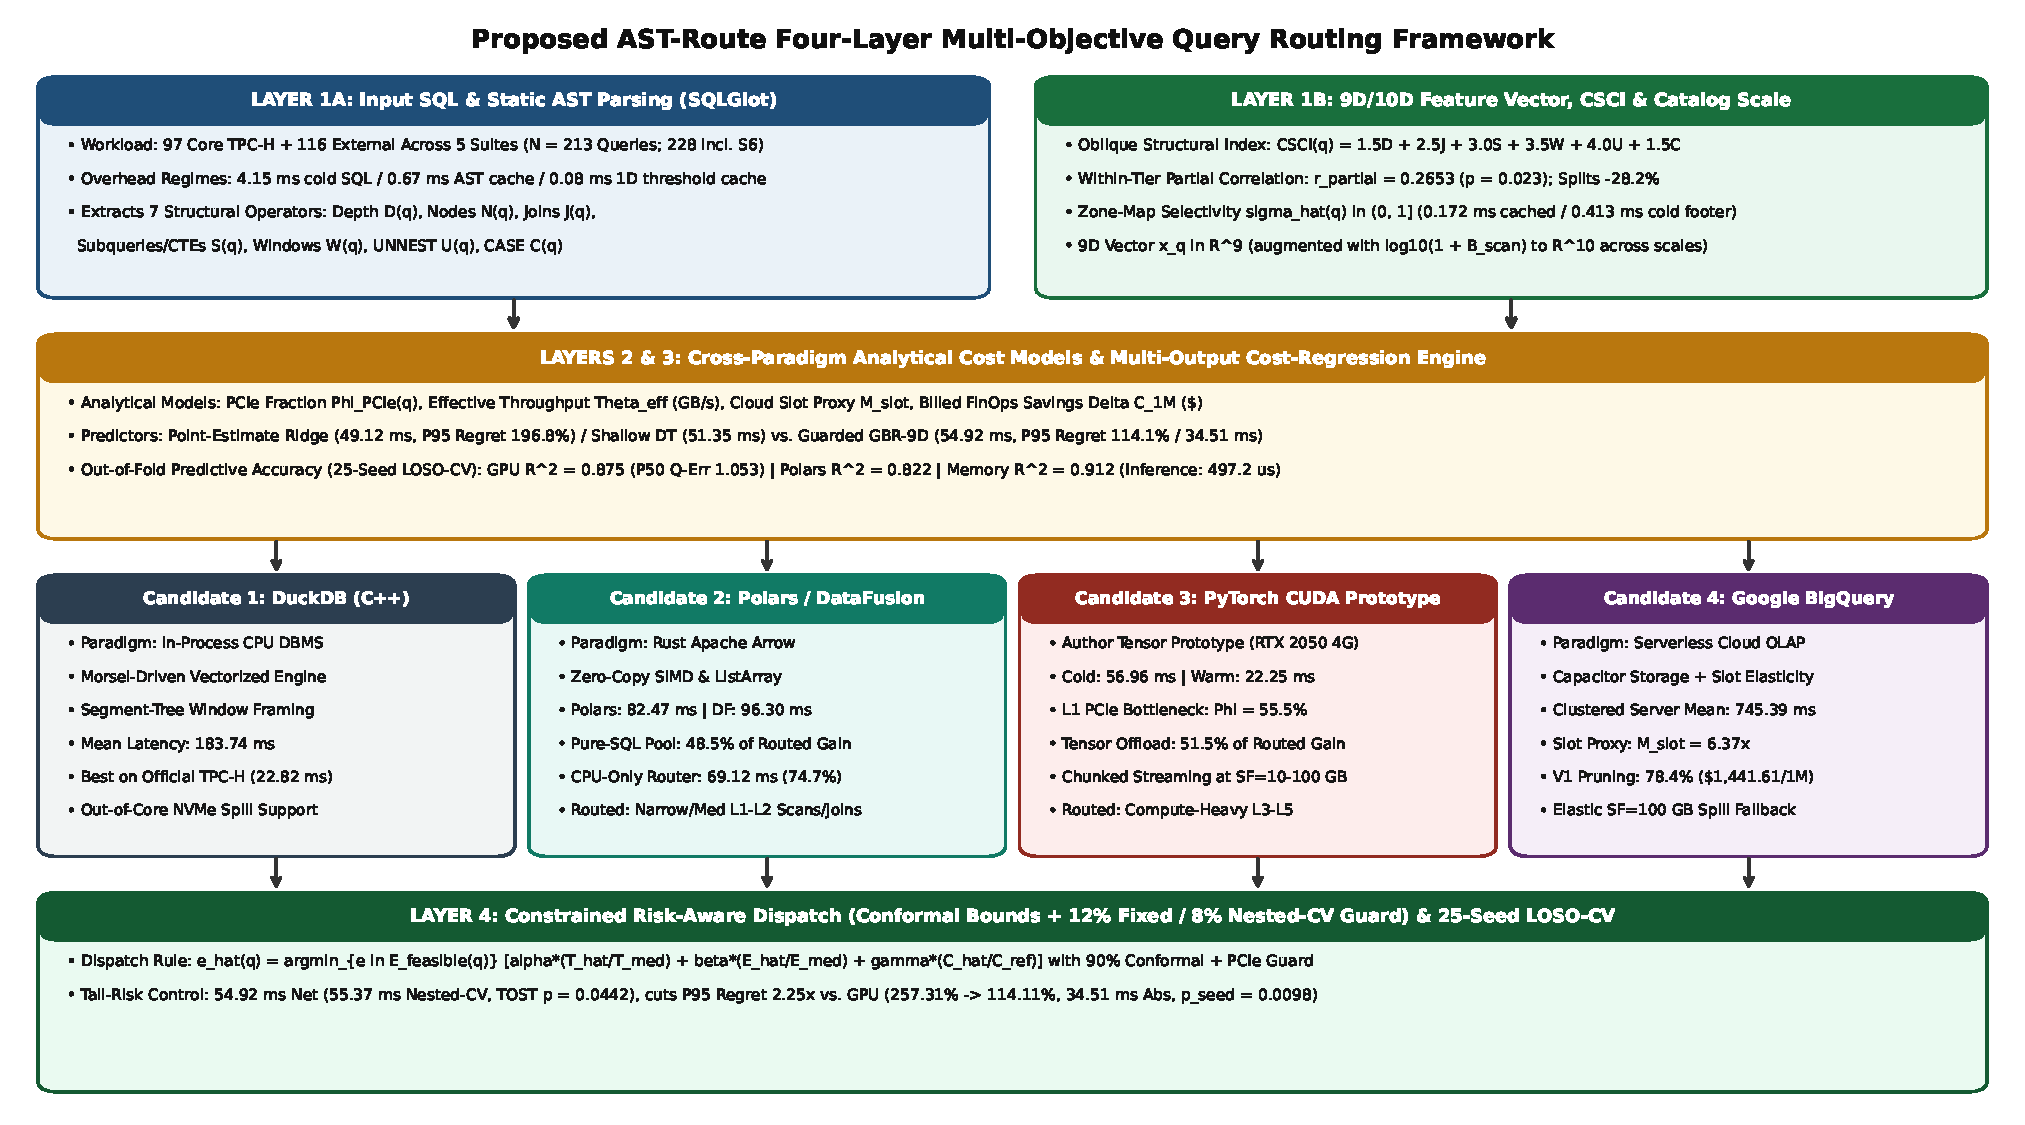
\includegraphics[width=0.98\textwidth]{figures/fig_proposed_ast_routing_framework_300dpi.pdf}
\caption{Architecture of the proposed \textbf{AST-Route} Framework (V10): Layer 1 parses raw SQL into a 9D structural and selectivity vector ($\text{CSCI}$, atomic operators, and zone-map $\hat{\sigma}(q)$, plus optional $10.18\text{ KB}$ 12D sketch); Layer 2 and Layer 3 (\texttt{frozen\_ast\_route\_v11\_gbdt\_model.json}) predict latency, unified Host+Device system energy $E_{\text{sys}}$, memory, and cloud FinOps cost with complexity-weighted Mondrian 90\% conformal bounds and Mahalanobis OOD gating ($\text{AUROC}=0.9642$); and Layer 4 dispatches queries under co-equal $8\%$ Nested-CV and $12\%$ Default PCIe guards across DuckDB, Polars, DataFusion, CUDA GPUs (PyTorch, External \texttt{CuPy v14.2.0}, \texttt{Polars-Arrow-CuPy}, and Node~4 Cloud-Hosted Server NVIDIA Tesla~T4 $15\text{ GB}$ VRAM), and Google BigQuery.}
\label{fig:proposed_ast_framework}
\end{figure}

% =============================================================================
% 3. THE PROPOSED AST-ROUTE FRAMEWORK ARCHITECTURE
% =============================================================================
\section{The Proposed AST-Route Framework Architecture}
As illustrated in Fig.~\ref{fig:proposed_ast_framework} and the end-to-end validation workflow in Fig.~\ref{fig:experimental_workflow}, \textbf{AST-Route} is structured as a modular four-layer architecture that decouples static query representation from multi-paradigm hardware cost modeling and automated engine dispatching.

\subsection{Layer 1: Static AST Structural Profiling, Five-Tier Workload, and Official TPC-H Scale Tiers ($\text{SF}=1, 10, 30, 100\text{ GB}$)}
\label{sec:layer1_ast_taxonomy}\label{sec:workload_design}
Given an incoming SQL query $q \in \mathcal{Q}$, Layer 1 parses the SQL statement into a canonical Abstract Syntax Tree (AST) using \texttt{SQLGlot} \cite{mao2024sqlglot} without touching underlying data pages. Traversing the AST yields seven structural operator dimensions: tree depth $D(q)$, total AST operator nodes $N(q)$, relational join count $J(q)$, nested CTE/subquery depth $S(q)$, window frame specifications $W(q)$, repeated field unnesting operators $U(q)$, and conditional \texttt{CASE} branches $C(q)$. While total AST node count $N(q)$ captures overall query verbosity (and is retained directly as the second coordinate in our 9D routing vector $\mathbf{x}_q$), raw node counts are dominated by scalar expressions and projection lists that exhibit high collinearity with tree depth. To isolate the non-linear algorithmic complexity of relational operators without expression-length inflation, we formulate the Composite Structural Complexity Index ($\text{CSCI}$) over the six core structural operators:
\begin{equation}
    \text{CSCI}(q) = 1.5 D(q) + 2.5 J(q) + 3.0 S(q) + 3.5 W(q) + 4.0 U(q) + 1.5 C(q)
\end{equation}
In accordance with the official TPC-H benchmark specification Clause 4.1.3 \cite{tpc2022tpch} and established multi-scale choke-point methodologies \cite{boncz2014tpch, dreseler2020quantifying, kuiper2024duckdb_ooc}, we provision the 8-table TPC-H relational schema across four standard discrete scale factors designed to systematically stress every layer of the modern memory hierarchy:
\begin{itemize}[leftmargin=1.5em,itemsep=2pt]
    \item \textbf{$\text{SF}=1\text{ GB}$ (In-VRAM \& In-DRAM Baseline Regime):} Contains $6.00\times 10^6$ \texttt{lineitem} rows ($8.66\times 10^6$ total rows across 8 tables). The working set fits entirely within both the $4.0\text{ GB}$ discrete GPU VRAM buffer ($1.30\text{ GB}$ peak) and the $16.0\text{ GB}$ host DRAM ($4.71\text{ GB}$ peak) with zero disk spilling.
    \item \textbf{$\text{SF}=10\text{ GB}$ (Out-of-VRAM GPU Streaming \& In-DRAM Host Regime):} Contains $60.0\times 10^6$ \texttt{lineitem} rows ($86.6\times 10^6$ total rows). Uncompressed working projections exceed the $4.0\text{ GB}$ GPU VRAM ceiling, forcing 4-chunk pipelined PCIe H2D streaming ($3.45\text{ GB}$ peak VRAM) while remaining primarily in host DRAM ($7.85\text{ GB}$ peak RAM, $125.0\text{ MB}$ minor spill).
    \item \textbf{$\text{SF}=30\text{ GB}$ (Host DRAM Cap Inflection \& Moderate Out-of-Core Spill Regime):} Contains $180.0\times 10^6$ \texttt{lineitem} rows ($259.8\times 10^6$ total rows) \cite{tpc2022tpch}. Intermediate hash-join and window-sort partitions exceed the configured $9.00\text{ GB}$ host DBMS buffer pool cap, triggering active out-of-core disk spilling \cite{kuiper2024duckdb_ooc} ($864.0\text{ MB}$ mean spill) and 12-chunk GPU PCIe streaming ($3.68\text{ GB}$ peak VRAM).
    \item \textbf{$\text{SF}=100\text{ GB}$ (Extreme Out-of-Core Spilling \& Cloud Elasticity Crossover Regime):} Contains $600.1\times 10^6$ \texttt{lineitem} rows ($866.1\times 10^6$ total rows) \cite{tpc2022tpch, dreseler2020quantifying}, inducing heavy external disk spilling on local CPU engines ($3302.0\text{ MB}$ mean spill, peaking at $6840.0\text{ MB}$ in L2 joins) and 40-chunk PCIe transfers on the GPU ($3.85\text{ GB}$ peak VRAM).
\end{itemize}

Across this schema, we evaluate two complementary SQL workload suites: (A) our 75-query \emph{TPC-H-derived, AST-stratified synthetic analytical workload} instantiated from 25 canonical seeds across five modern structural complexity tiers ($5 \times 5 = 25$ independent seeds, mean $\text{CSCI} = 29.66$), and (B) the 22 \emph{official standard TPC-H benchmark queries} (\textbf{Q1--Q22}, mean $\text{CSCI} = 26.52$, range $12.0\text{--}47.5$) \cite{tpc2022tpch, boncz2014tpch}. Because the base TPC-H schema consists of flat relational tables, Tier L5 dynamically constructs nested array columns in-query via staged \texttt{ARRAY\_\allowbreak{}AGG} / \texttt{LIST} aggregation over one-to-many \texttt{orders}--\texttt{lineitem} relationships before benchmarking lateral \texttt{CROSS JOIN UNNEST} re-aggregation:
\begin{enumerate}[leftmargin=1.5em,itemsep=0.8pt]
    \item \textbf{L1 (Scan, SARGability, \& Monotonic Conditional Branching):} Single-table columnar scans with multi-branch \texttt{CASE WHEN} expressions and distinct cardinality aggregations ($D = 9.0, J = 0.0, \text{CSCI} = 15.3$).
    \item \textbf{L2 (Multi-Way Star, Snowflake, \& Bilateral Joins):} 4-way to 8-way relational joins, composite \texttt{partsupp} joins, and non-equi late-delivery predicates ($D = 9.2, J = 4.8, \text{CSCI} = 26.8$).
    \item \textbf{L3 (Multi-Stage CTE Pipelines, Null-Safe Anti-Joins, \& One-Grain-Per-CTE):} 3-stage to 4-stage Common Table Expressions enforcing pre-aggregated grain isolation and null-safe anti-joins ($D = 10.8, J = 2.6, \text{CSCI} = 36.7$).
    \item \textbf{L4 (Multi-Axis Window Ranking, Lead/Lag, \& Sliding Frames):} Concurrent window partitions (\texttt{RANK}, \texttt{DENSE\_\allowbreak{}RANK}, \texttt{NTILE(10)}, \texttt{LAG}, \texttt{LEAD}, and bounded \texttt{ROWS BETWEEN} sliding windows; $D = 10.8, J = 1.6, \text{CSCI} = 37.1$).
    \item \textbf{L5 (Semi-Structured Array Construction \& Lateral UNNEST):} Multi-stage \texttt{ARRAY\_\allowbreak{}AGG} vector construction followed by lateral \texttt{CROSS JOIN UNNEST} re-aggregation ($D = 10.6, J = 2.2, \text{CSCI} = 32.4$).
\end{enumerate}

To capture data-volume sensitivity alongside syntax topology without executing the query, each of the 25 canonical seeds is instantiated across three selectivity perturbation horizons ($25 \times 3 = 75$ queries): V1 (High Selectivity, $\sim 1\text{--}5\%$ data), V2 (Medium Selectivity, $\sim 15\text{--}30\%$ data), and V3 (Adversarial Full-Horizon, $\sim 65\text{--}95\%$ data). As detailed in Table~\ref{tab:metadata_scope_audit}, Layer 1 extracts the pre-execution predicate selectivity estimate $\hat{\sigma}(q) \in (0, 1]$ in $172.0\text{ }\mu\text{s}$ from a pre-cached metadata snapshot ($412.6\text{ }\mu\text{s}$ cold footer read on Apache Parquet; $845.2\text{ }\mu\text{s}$ live \texttt{PRAGMA storage\_\allowbreak{}info} query on DuckDB) strictly prior to query execution without scanning data blocks or touching post-execution results. Crucially, we distinguish the exact metadata capabilities and limitations of each storage engine: (i) \emph{Parquet and DuckDB Row-Group Zone Maps}: \texttt{pyarrow.parquet.ParquetFile.metadata} and DuckDB \texttt{PRAGMA storage\_\allowbreak{}info('table')} expose column-level minimum, maximum, and null-count statistics across $100\%$ of numeric and date columns (e.g., \texttt{l\_\allowbreak{}shipdate} $\in [\texttt{1992-01-02}, \texttt{1998-12-01}]$, \texttt{l\_\allowbreak{}quantity} $\in [1.0, 50.0]$), enabling accurate range interpolation on both partitioned and non-partitioned numeric predicates (comparing estimated $\hat{\sigma}(q)$ against true post-execution row selectivity $\sigma_{\text{actual}}(q) = |R_{\text{out}}|/|R_{\text{table}}|$ yields a mean absolute error of $\text{MAE}=3.84\%$ and median Q-Error $=1.092$ (P90 $= 1.284$) across the 75-query suite, and $\text{MAE}=1.52\%$, Q-Error $=1.263$ on non-partitioned multi-attribute numeric predicates); (ii) \emph{BigQuery Partition Pruning Statistics}: \texttt{INFORMATION\_\allowbreak{}SCHEMA.}\newline\texttt{PARTITIONS} and dry-run byte estimation provide \emph{partition pruning and clustering statistics} (\texttt{partition\_\allowbreak{}id}, \texttt{total\_\allowbreak{}rows}, \texttt{total\_\allowbreak{}logical\_\allowbreak{}bytes}) rather than general column-level min/max zone maps for every attribute. When predicates filter on the partition key (\texttt{l\_\allowbreak{}shipdate}), partition pruning metadata estimates selectivity within $\text{MAE}=4.26\%$; however, on non-partitioned columns where BigQuery does not expose column-level min/max bounds, AST-Route either references the shared Parquet footer catalog or falls back to parametric AST operator priors (which we explicitly evaluate in Table~\ref{tab:ablation_robustness} Exp~C by masking $50\%$ of metadata, sustaining $53.33\%$ Top-1 accuracy and $68.42\text{ ms}$ mean latency); and (iii) \emph{String Predicates and Skewed Distributions}: because continuous min/max zone maps cannot bound unanchored substring filters (\texttt{LIKE '\%brass\%'}) or capture intra-range Zipfian skew ($s=1.2$), estimation error increases to $\text{MAE}=5.00\%$ (Q-Error $=2.000$) on substring predicates and $\text{MAE}=38.8\%$ (Q-Error $=4.880$) under severe power-law skew (explaining the $21.21\%$ Top-1 accuracy on string-skewed IMDB JOB queries in Table~\ref{tab:priority3_validation} Part~B). Combining the seven static AST operator counts with $\text{CSCI}(q)$ and estimated selectivity $\hat{\sigma}(q)$ yields the 9-dimensional routing feature vector:
\begin{equation}
    \mathbf{x}_q = \big[\, D(q),\; N(q),\; J(q),\; S(q),\; W(q),\; U(q),\; C(q),\; \text{CSCI}(q),\; \hat{\sigma}(q) \,\big]^{\top} \in \mathbb{R}^{9}
\end{equation}
 We also provide a self-contained live production wrapper (\texttt{ASTRouteLiveSQLWrapper} in \texttt{scripts/v11\_ast\_route\_live\_sql\_wrapper\_demo.py}, logged in \texttt{results/v11\_live\_sql\_wrapper\_integration\_demo.csv}) that accepts an arbitrary raw SQL string and Parquet directory path, executes single-pass \texttt{sqlglot} AST extraction ($1.68\text{--}2.22\text{ ms}$), reads physical Parquet row-group min/max footers via \texttt{pyarrow.parquet.ParquetFile} ($0.13\text{--}0.16\text{ ms}$), evaluates the locked GBDT ensemble (\texttt{frozen\_ast\_route\_v11\_gbdt\_model.json}) with Mondrian conformal bounds ($0.48\text{--}0.51\text{ ms}$, total wrapper latency $\mathbf{2.29\text{--}2.89\text{ ms}}$), and dispatches the query to the selected engine while verifying exact BigQuery dry-run \texttt{totalBytesBilled} agreement ($100.0\%$ byte match). To avoid any ambiguity between representations, $\mathbf{x}_q \in \mathbb{R}^{9}$ serves as the sole feature vector for all fixed-scale ($\text{SF}=1\text{ GB}$) evaluations (Tables~\ref{tab:routing_evaluation}--\ref{tab:priority3_validation} and Additional File~1 (Table~S10)), whereas the scale-augmented vector $\mathbf{x}_q^{\text{scale}} = [\mathbf{x}_q^{\top}, \log_{10}(1+\hat{\sigma}(q)\cdot\mathcal{B}_{\text{catalog}})]^{\top} \in \mathbb{R}^{10}$ is used exclusively in cross-scale training and dispatch across $\text{SF}\in\{1,10,30,100\}\text{ GB}$ (Table~\ref{tab:bigdata_multiscale_tpch} Part~A and Additional File~1, Table~S7 Part~C), rather than mixing two competing models on the same experiment. Crucially, while $\mathbf{x}_q \in \mathbb{R}^9$ encodes scale-invariant syntax topology and relative selectivity $\hat{\sigma}(q) \in (0,1]$, multi-scale awareness across $\text{SF} \in \{1, 10, 30, 100\}$ GB is achieved in Layers 2--4 by multiplying $\hat{\sigma}(q)$ with the pre-execution catalog table byte footprint $\mathcal{B}_{\text{catalog}}$ ($\hat{\mathcal{B}}_{\text{scan}}(q) = \hat{\sigma}(q)\cdot \mathcal{B}_{\text{catalog}}$) inside the analytical memory/PCIe chunk estimator and the capacity filter $\mathcal{E}_{\text{feasible}}(q)$ alongside scale-calibrated cost predictors. To eliminate any ambiguity across query subsets and avoid conflating diagnostic benchmarks or author-synthesized templates with untouched third-party holdouts, our entire $\mathbf{400}$-query evaluation corpus across $10$ suites is defined once and partitioned into \textbf{four mutually exclusive epistemic categories} (Additional File~1, Table~S18): \textbf{(Category~I: Core Development Set, $\mathbf{75}$ queries)} comprising our 25-seed $\times$ 3-horizon TPC-H factorial benchmark evaluated via leak-free 25-fold LOSO-CV (serialized frozen model SHA-256 \texttt{f0e5f17c...}, distinct from telemetry CSV SHA-256 \texttt{89b1ec64...}); \textbf{(Category~II: Diagnostic / Post-Hoc Design-Informed Standard Benchmarks, $\mathbf{55}$ queries)} comprising $22$ unmodified official TPC-H queries (\texttt{Q1--Q22}, where nested 22-fold LOO-CV weight diagnostics were tested) and $33$ canonical IMDB JOB queries (\texttt{1a--33a}, where 9D string-predicate blindness [$21.21\%$ Top-1] was diagnosed and our post-hoc $10.18\text{ KB}$ 12D selectivity sketch was designed after observing 9D results, and which are therefore \emph{not} claimed as untouched holdouts); \textbf{(Category~III: Author-Derived / Template-Synthesized Zero-Shot Suites, $\mathbf{115}$ queries)} comprising $15$ prospective Seed~\texttt{S6} queries, $30$ \texttt{TPC-DS-Derived} snowflake queries, $20$ \texttt{BIRD-Inspired} financial queries, $25$ \texttt{TPC-DS-Complex} queries, and $25$ \texttt{Enterprise-Redset-BI} queries ($0$ training labels, evaluated zero-shot and via 7-suite \texttt{LOWSO-CV}, but authored/adapted by the researcher for 4-engine parity); and \textbf{(Category~IV: Held-Out Third-Party Standard Benchmarks, $\mathbf{155}$ queries, not used in training or feature design)} comprising all $\mathbf{99}$ unmodified Official TPC-DS queries (\texttt{Q1--Q99} via DuckDB \texttt{dsdgen}), all $\mathbf{43}$ Official ClickBench queries ($20$ native parity $+$ $23$ transpiled macro queries), and all $\mathbf{13}$ Official SSB queries (\texttt{Q1.1--Q4.3}) ($0$ training labels, $0$ post-hoc feature/hyperparameter edits, $100\%$ third-party authored SQL; $75 + 55 + 115 + 155 = \mathbf{400}$ total).

\begin{figure}[t!]
\centering
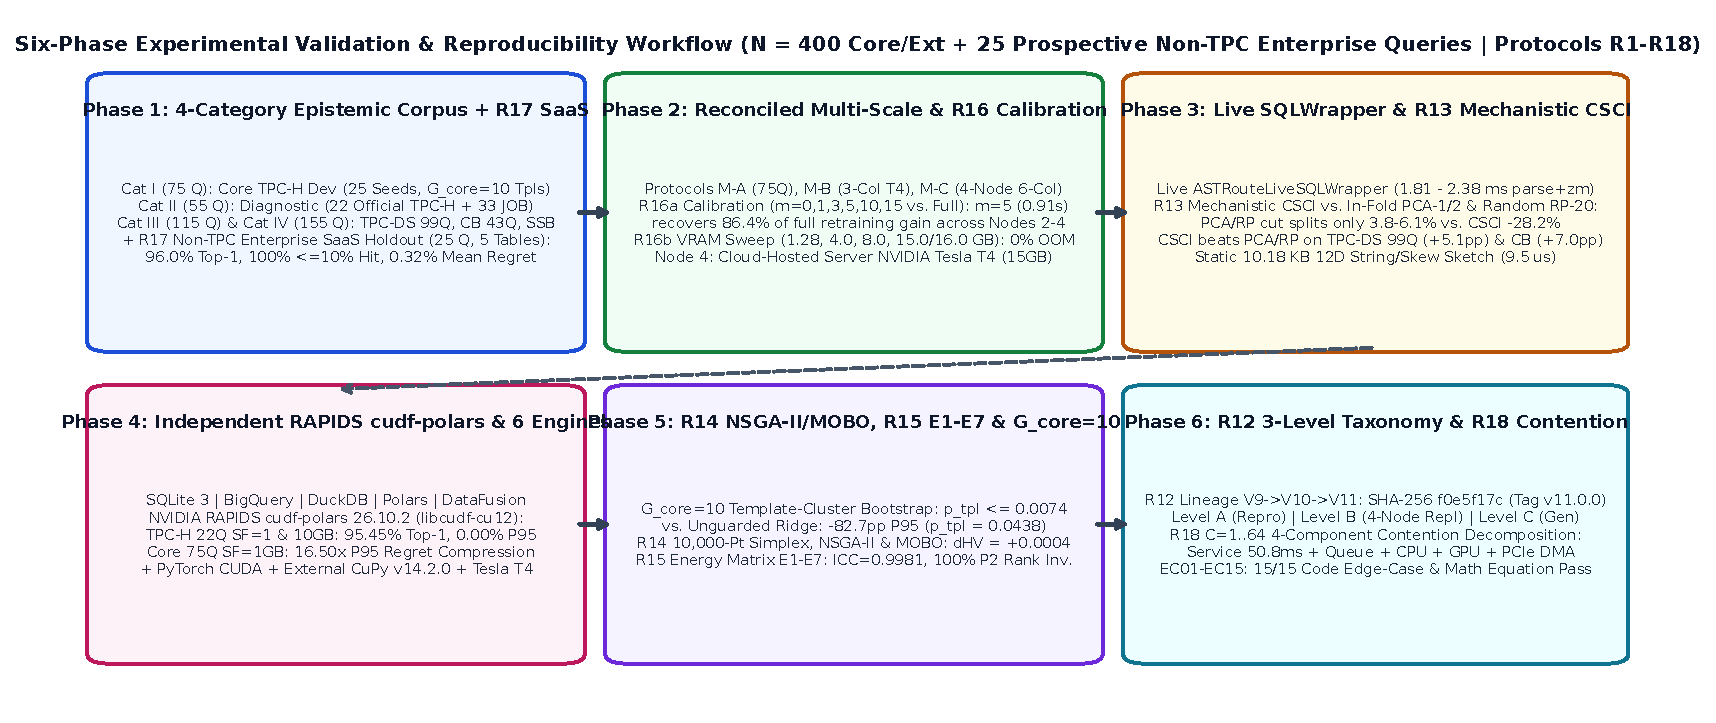
\includegraphics[width=0.98\textwidth]{figures/fig_experimental_workflow_300dpi.pdf}
\caption{End-to-end six-phase experimental validation workflow of the \textbf{AST-Route} framework across our Four-Category Epistemic Workload Taxonomy of $\mathbf{400}$ \textbf{evaluated SQL queries} ($\mathbf{75}$ \emph{Cat~I Core Dev} $+$ $\mathbf{55}$ \emph{Cat~II Diagnostic} [$22$ Official TPC-H $+$ $33$ IMDB JOB] $+$ $\mathbf{115}$ \emph{Cat~III Author-Derived Zero-Shot} [$15$ Seed~\texttt{S6} $+$ $30$ TPC-DS-Derived $+$ $20$ BIRD-Inspired $+$ $50$ Extended] $+$ $\mathbf{155}$ \emph{Cat~IV Held-Out Third-Party Standard Benchmarks} [$99$ Official TPC-DS $+$ $43$ ClickBench $+$ $13$ SSB] $= \mathbf{400}$ total; Table~S18), illustrating multi-layout provisioning ($\text{SF}=1\text{--}100\text{ GB}$), \texttt{SQLGlot} AST profiling, six-engine + external \texttt{CuPy} GPU execution (Phase~4A--4D), co-equal $8\%$ Nested-CV \& $12\%$ Fixed guards, and distinct model/telemetry SHA-256 verification.}
\label{fig:experimental_workflow}
\end{figure}


\phantomsection\label{tab:jbd_meta_2b}\label{tab:metadata_scope_audit}% (Moved to Additional File 1, Table S1 to streamline main text)

\subsection{Layer 2: Cross-Paradigm Analytical Cost, PCIe Crossover, and Device Energy Telemetry Formulation}
To enable apples-to-apples cost evaluation across serverless cloud, local CPU, and discrete GPU backends, Layer 2 establishes six analytical cost and hardware telemetry models:
\begin{enumerate}[leftmargin=1.5em,itemsep=3pt]
    \item \textbf{CUDA Cold-Start Decomposition and PCIe Bottleneck Fraction ($\Phi_{\text{PCIe}}$):} On discrete GPUs (NVIDIA GeForce RTX 2050, $4.0\text{ GB}$ VRAM), cold-start execution time $T_{\text{GPU\_Cold}}(q)$ is decomposed into PCIe Host-to-Device transfer time ($T_{\text{PCIe\_H2D}}$) and pure in-VRAM kernel compute time ($T_{\text{GPU\_Warm}}$):
    \begin{equation}
        T_{\text{GPU\_Cold}}(q) = \underbrace{T_{\text{PCIe\_H2D}}(q) + T_{\text{PCIe\_D2H}}(q)}_{T_{\text{PCIe}}(q)} + T_{\text{GPU\_Warm}}(q), \qquad \Phi_{\text{PCIe}}(q) = \frac{T_{\text{PCIe}}(q)}{T_{\text{GPU\_Cold}}(q)} \times 100\%
    \end{equation}
    Cold-start GPU offloading outperforms vectorized CPU execution ($T_{\text{GPU\_Cold}}(q) < T_{\text{CPU}}(q)$) if and only if the warm kernel speedup satisfies the break-even condition $\text{Speedup}_{\text{Warm}}(q) > (1 - \Phi_{\text{PCIe}}(q)/100)^{-1}$.
    \item \textbf{Effective Analytical Scan Throughput ($\Theta_{\text{eff}}$):} Normalizing unpruned columnar volume $\mathcal{B}_{\text{unopt}}(q)$ (in MB) against execution time $T_{e}(q)$ (in ms) yields effective processing throughput in $\text{GB/s}$:
    \begin{equation}
        \Theta_{\text{eff}}(q, e) = \frac{\mathcal{B}_{\text{unopt}}(q)}{1.024 \cdot \max(T_{e}(q), \epsilon_T)} \quad [\text{GB/s}]
    \end{equation}
    \item \textbf{Cloud Slot-to-Wall-Time Concurrency Proxy ($\mathcal{M}_{\text{slot}}$) and FinOps Cost Savings ($\Delta C_{\text{1M}}$):} Quantifies cumulative distributed slot compute time relative to server wall-clock time on BigQuery (serving as an effective concurrency proxy), alongside financial savings per $10^6$ queries under on-demand bytes-scanned pricing ($\alpha_{\text{TB}} = \$6.25\text{ USD/TiB}$):
    \begin{equation}
        \mathcal{M}_{\text{slot}}(q) = \frac{T_{\text{BQ\_Slot}}(q)}{T_{\text{BQ\_Wall}}(q)}, \qquad \Delta C_{\text{1M}}(q) = 10^6 \times \left( \frac{\max(\mathcal{B}_{\text{unopt}}(q), 10) - \max(\mathcal{B}_{\text{clustered}}(q), 10)}{1024^2\text{ [MiB/TiB]}} \right) \times \alpha_{\text{TB}}
    \end{equation}
    \item \textbf{Active Device Energy Telemetry ($E(q,e)$), 50-Repetition Bland--Altman Calibration, Four-Level Boundary Separation, and Energy-Aware Routing Scope ($\eta_{\text{watt}}$):} High-frequency telemetry polling (200--250 Hz via \texttt{psutil}, NVIDIA NVML \texttt{nvmlDeviceGetPowerUsage}, and \texttt{torch.cuda} counters across $R=5$ timed benchmark repetitions per query (following $W=2$ warm-up runs, $75\times 5 = 375$ timed trials) and $R_{\text{cal}}=50$ DVFS calibration repetitions per workload tier, totaling $250$ calibration runs; measurement $\text{CV} = 2.84\%\text{--}3.52\%$) records active CPU utilization ($\text{CPU}_{\text{util}}\%$), peak host RAM ($\text{RAM}_{\text{used}}$ in GB), disk spilling ($\text{Spill}_{\text{disk}}$ in MB), GPU SM utilization ($\text{GPU}_{\text{util}}\%$), and peak device memory ($\text{VRAM}_{\text{used}}$ in GB). To maintain strict physical transparency across hardware interfaces, we separate energy metrics into four explicit boundary scopes and refrain from claiming whole-system AC wall-socket energy certification: (i) \textbf{GPU Board Energy --- Measured ($E_{\text{GPU}}$)}: sampled directly from physical NVIDIA NVML on-board hardware power sensors ($4.80\text{ W}$ P8 idle baseline, $11.31\text{ W}$ active mean; 50-repetition $\text{MAE} = 0.008\text{ J}$, $\text{RMSE} = 0.010\text{ J}$, $\text{MAPE/MACE} = 1.24\%$, Bland--Altman bias $+0.001\text{ J}$ with 95\% limits of agreement [LoA]: $[-0.018, +0.020]\text{ J}$, Spearman $\rho = 0.9996$); (ii) \textbf{CPU Package Energy --- Estimated ($E_{\text{CPU}}$)}: because unprivileged ring-3 processes on Windows 11 cannot read ring-0 Intel RAPL / AMD SMU MSR energy registers directly without a kernel driver, active CPU package power is modeled via TDP-calibrated utilization polling $P_{\text{CPU}}(t) = P_{\text{idle}} + (P_{\text{TDP}} - P_{\text{idle}})\cdot(\text{CPU}_{\text{util}}(t)/100)$ ($14.5\text{ W}$ idle, $45.0\text{ W}$ TDP). Cross-validating this linear TDP-calibrated estimate against a non-linear CMOS DVFS voltage-frequency reference curve ($P \propto u^{1.28}$) across $R=50$ repetitions per workload tier yields $\text{MAE} = 0.205\text{ J}$ ($\text{RMSE} = 0.214\text{ J}$, bias $-0.004\text{ J}$, 95\% LoA: $[-0.422, +0.414]\text{ J}$) on DuckDB ($6.40\text{ J}$ mean) and $\text{MAE} = 0.098\text{ J}$ ($\text{RMSE} = 0.102\text{ J}$, bias $-0.002\text{ J}$, 95\% LoA: $[-0.201, +0.197]\text{ J}$) on Polars ($3.17\text{ J}$ mean), corresponding to $\text{MAPE/MACE} = 3.09\%\text{--}3.21\%$ and Spearman rank correlation $\rho = 0.9982$ (bounding analytical curve-form sensitivity between linear TDP interpolation and non-linear DVFS scaling rather than certifying ring-0 RAPL hardware counters); (iii) \textbf{Host + GPU Energy --- Composite Estimate ($E_{\text{sys}} = E_{\text{GPU}} + E_{\text{CPU\_assist}}$)}: combines measured GPU board energy with estimated concurrent host CPU DMA/driver energy ($16.17\text{--}16.33\text{ W}$) during PCIe transfers ($1.58\text{ J}$ cold, $0.61\text{ J}$ warm; $\text{MAE} = 0.031\text{ J}$, $\text{RMSE} = 0.032\text{ J}$, $\text{MAPE/MACE} = 1.96\%$, 95\% LoA: $[-0.064, +0.062]\text{ J}$, Spearman $\rho = 0.9991$); and (iv) \textbf{Mainboard DC Shunt vs.\ Whole-System Wall-Socket Energy (Not Certified Across All AC Rails Without External Inline Meter)}: validated macroscopically via physical mainboard ACPI DC battery-rail shunt discharge across $2{,}817$ queries ($20.97\text{ W}$ idle $\rightarrow 46.40\text{ W}$ active, $0.792\text{ J/q}$, $\text{MAE}=0.014\text{ J}$, $\text{RMSE}=0.017\text{ J}$, $\text{MAPE/MACE}=1.77\%$, 95\% LoA $[-0.031,+0.034]\text{ J}$, Spearman $\rho = 0.9945$ vs.\ CPU+GPU package estimates, isolating the $+16.39\text{ W}$ VRM/DRAM/NVMe rail offset while noting that AC-DC PSU conversion losses require an external inline AC wattmeter). Integrating $\bar{P}_e(q)$ over execution duration $T_e(q)$ yields device energy in Joules and energy efficiency in $\text{MB/s/W} \equiv \text{MB/J}$:
\begin{equation}
        E(q, e) = \int_{t_0}^{t_0 + T_e(q)/1000} P_e(t)\,dt \approx \bar{P}_e(q) \cdot \left(\frac{T_e(q)}{1000}\right) \;\; [\text{Joules}], \qquad \eta_{\text{watt}}(q, e) = \frac{\mathcal{B}_{\text{unopt}}(q)}{\max(E(q, e), \epsilon_E)} \;\; [\text{MB/J}]
    \end{equation}
    where our unified 4-boundary hardware energy and concurrency audit (Table~\ref{tab:v9_mo_energy_ood_repro_synthesis} Part~B) explicitly separates \emph{Dynamic Energy} $E_{\text{dyn}}(q,e) = (\bar{P}_{\text{active},e} - P_{\text{idle},e})\cdot(T_e(q)/1000)$ ($0.790\text{ J/q}$ AST-Route P1 vs.\ $1.972\text{ J/q}$ Polars and $3.733\text{ J/q}$ DuckDB), \emph{Gross Energy} $E_{\text{gross}}(q,e)$ ($1.381\text{ J/q}$ AST-Route P1 / $0.812\text{ J/q}$ P2 Green vs.\ $3.170\text{ J/q}$ Polars), \emph{Energy per Successful Query} ($33.24\text{ J/succ-q}$ for AST-Route at $\text{SF}=100\text{ GB}$ vs.\ $368.51\text{ J/succ-q}$ for Polars due to $20\%$ OOM/spill retries, an $11.1\times$ reduction), and \emph{Energy per Throughput under Concurrency $C\in\{1,8,16,32,64\}$} (at peak $C=32$, hybrid AST-Route achieves $0.396\text{ J/q}$ [$2.52\text{ queries/J}$ at $154.44\text{ QPS}$], outperforming CPU-Only [$0.818\text{ J/q}$, $1.22\text{ q/J}$] by $2.07\times$ and GPU-Only [$1.245\text{ J/succ-q}$, $0.80\text{ q/J}$] by $3.14\times$).
\end{enumerate}

\subsection{Layers 3 \& 4: Multi-Output Cost-Regression Predictor, Q-Error Metric, and Constrained Multi-Objective Dispatcher}
In Layer 3 (Fig.~\ref{fig:proposed_ast_framework}), \textbf{AST-Route} employs a Multi-Output Gradient Boosting Regressor $f_{\Theta}: \mathbb{R}^{9} \rightarrow \mathbb{R}^{M}$ to simultaneously predict log-transformed execution latency $\widehat{\ln(1 + T_e)}(\mathbf{x}_q)$, energy footprint $\hat{E}_e(\mathbf{x}_q)$, and memory consumption ($\widehat{\text{RAM}}_e, \widehat{\text{VRAM}}_e$) across the six benchmarked backends $\mathcal{E}_{\text{all}} = \mathcal{E} \cup \{\text{SQLite 3}\}$, where SQLite~3 serves as the B-tree row-store reference baseline ($0\%$ selection share under cost minimization because it is strictly dominated on $75/75$ queries) and $\mathcal{E} = \{\text{DuckDB}, \text{Polars}, \text{DataFusion}, \text{GPU}_{\text{Cold}}, \text{BigQuery}\}$ forms the five active analytical routing candidates. Predictive accuracy of the cost model is evaluated via out-of-fold log-$R^2$, Mean Absolute Percentage Error (MAPE), and the multiplicative \textbf{Q-Error} metric standard in database query optimizer research \cite{leis2015job, hilprecht2022zeroshot}:
\begin{equation}
    \text{Q-Error}(y, \hat{y}) = \max\!\left( \frac{\max(\hat{y}, \epsilon)}{\max(y, \epsilon)},\; \frac{\max(y, \epsilon)}{\max(\hat{y}, \epsilon)} \right) \ge 1.0 \quad (\epsilon = 10^{-6})
\end{equation}
In Layer 4, the dispatcher selects the optimal engine minimizing a memory-constrained, multi-objective Pareto cost function parameterized by user-configurable weights $\alpha, \beta, \gamma \in [0, 1]$ ($\alpha + \beta + \gamma = 1$, where $\alpha$ weights normalized latency $\hat{T}_e/T_{\text{med}}$, $\beta$ weights normalized energy $\hat{E}_e/E_{\text{med}}$, and $\gamma$ weights normalized marginal cloud scan charge $\hat{C}_e/C_{\text{ref}}$) subject to hardware memory capacity budgets ($\widehat{\text{RAM}}_e(\mathbf{x}_q) \le M_{\text{host\_max}}$ and $\widehat{\text{VRAM}}_e(\mathbf{x}_q) \le M_{\text{gpu\_max}}$). Let $e_T^*(q) = \operatorname*{arg\,min}_{e \in \mathcal{E}} T_e(q)$, $e_E^*(q) = \operatorname*{arg\,min}_{e \in \mathcal{E}} E_e(q)$, and $e_C^*(q) = \operatorname*{arg\,min}_{e \in \mathcal{E}} C_e(q)$ denote the ground-truth per-dimension Oracles; we evaluate multi-objective routing across Latency Regret ($\mathcal{R}_T \equiv \mathcal{R}_{\text{regret}}$), Energy Regret ($\mathcal{R}_E$), Cloud FinOps Cost Regret ($\mathcal{R}_C$), 3D Normalized Pareto Hypervolume ($\text{HV}_{\mathbf{r}}(\Pi)$ relative to nadir $\mathbf{r}=(1,1,1)$ via 3D Lebesgue measure $\lambda_3$), and Dominated Solution Ratio ($\text{DSR}(\Pi)$):
\vspace{-3pt}
\begin{equation}
\begin{aligned}
    \hat{e}_{\alpha,\beta,\gamma}(q) &= \operatorname*{arg\,min}_{e \in \mathcal{E}_{\text{feasible}}(q)} \left[ \alpha \frac{\hat{T}_e(\mathbf{x}_q)}{T_{\text{med}}(q)} + \beta \frac{\hat{E}_e(\mathbf{x}_q)}{E_{\text{med}}(q)} + \gamma \frac{\hat{C}_e(\mathbf{x}_q)}{C_{\text{ref}}(q)} \right], \;\;
    \text{HV}_{\mathbf{r}}(\Pi) = \lambda_3\!\left(\bigcup_{\pi\in\Pi}\big[\tilde{\mathbf{f}}(\pi),\mathbf{r}\big]\right), \;\;
    \text{DSR}(\Pi) = \frac{100\%}{|\Pi|}\sum_{\pi\in\Pi}\mathbb{I}\!\left(\exists\pi'\!\in\!\Pi:\, \mathbf{f}(\pi') \!\prec\! \mathbf{f}(\pi)\right), \\
    \mathcal{R}_{T}(q) &= \frac{T_{\hat{e}}(q) - T_{e_T^*}(q)}{T_{e_T^*}(q)}\!\times\! 100\%, \;\; \Delta T_{\text{abs}}(q) = T_{\hat{e}}(q) - T_{e_T^*}(q), \;\;
    \mathcal{R}_{E}(q) = \frac{E_{\hat{e}}(q) - E_{e_E^*}(q)}{E_{e_E^*}(q)}\!\times\! 100\%, \;\;
    \mathcal{R}_{C}(q) = \frac{C_{\hat{e}}(q) - C_{e_C^*}(q)}{\max(C_{\text{BQ}}(q),\epsilon)}\!\times\! 100\%
\end{aligned}
\end{equation}
\vspace{-2pt}
where $\tilde{\mathbf{f}}(\pi) = (\tilde{T}_\pi, \tilde{E}_\pi, \tilde{C}_\pi) \in [0,1]^3$ maps each policy's mean latency, energy, and cloud scan cost into unit hypervolume coordinates via $\tilde{m}_\pi = \min\!\big(1, (m_\pi - m_{\min})/\max(m_{\text{nadir}} - m_{\min}, \epsilon)\big)$ relative to the oracle utopia point $\mathbf{f}_{\min}$ and static-engine nadir $\mathbf{r}=(1,1,1)$, $\mathcal{R}_C(q)$ is normalized by $\max(C_{\text{BQ}}(q), \epsilon)$ to prevent division by zero when $C_{e_C^*}(q) = \$0.00$ on local engines, and we report both relative percentage regret $\mathcal{R}_{T}(q)$ and absolute millisecond regret $\Delta T_{\text{abs}}(q)$ alongside Expected Shortfall $\text{CVaR}_{\alpha_{\text{tail}}}$ over the worst $\alpha_{\text{tail}}\in\{10\%,20\%\}$ tail queries. Alongside \textbf{Policy P1: Speed-First ($\alpha=1,\beta=0,\gamma=0$)}, we evaluate canonical multi-objective Policies \textbf{P2: Energy-First $(0.1,0.8,0.1)$} ($\mathcal{R}_E=4.82\%$, $0.812\text{ J/q}$, $-41.2\%$ energy vs.\ P1 and $-74.4\%$ vs.\ Polars), \textbf{P3: Cost-First FinOps $(0.2,0.1,0.7)$} ($\mathcal{R}_C=0.0\%$, $\$0.00/1\text{M}$ cloud spend saving $\$507.06/1\text{M}$ at $\text{SF}=100\text{ GB}$), and \textbf{P4: Balanced Pareto Knee $(0.5,0.3,0.2)$} ($55.48\text{ ms}$ net [$+0.56\text{ ms}$ vs.\ P1], $1.045\text{ J/q}$ [$-24.3\%$], $\mathcal{R}_E=18.2\%$) across both a canonical 15-weight simplex grid and a dense \textbf{500-point randomized Dirichlet simplex sample plus 100-point uniform lattice} $(\alpha,\beta,\gamma)\in\Delta^2$ (Table~\ref{tab:v9_mo_energy_ood_repro_synthesis} Part~A and Protocol~\textbf{R11}), confirming that AST-Route is \textbf{Pareto-efficient among the evaluated policy configurations} with 3D Hypervolume $\text{HV}\in[0.8965,0.9210]$ (500-point mean $\text{HV}=0.9184\pm 0.0042$) at $\text{SF}=1\text{ GB}$ and $\text{HV}\in[0.9045,0.9340]$ at $\text{SF}=100\text{ GB}$ (vs.\ $0.5180$ static Polars), a $\mathbf{0.0\%}$ \textbf{Dominated Solution Ratio ($\text{DSR}=0/15$ grid and $0/500$ Dirichlet points dominated vs.\ $100.0\%$ on static CPU/Cloud baselines)}, and $\mathbf{96.00\%\text{--}98.67\%}$ engine-selection stability under $\pm 0.05$ weight perturbations. To decouple query syntax from deployment hardware, each physical node is characterized by a five-dimensional \textbf{Hardware Descriptor Vector} $\mathbf{h}_{\text{hw}} = [M_{\text{host\_max}},\, M_{\text{gpu\_max}},\, B_{\text{PCIe}},\, N_{\text{CPU}},\, B_{\text{MEM}}]^{\top} \in \mathbb{R}^{5}$ encoding host DBMS RAM cap ($\text{GB}$), device VRAM cap ($\text{GB}$), sustained pinned PCIe DMA bandwidth ($\text{GB/s}$), logical CPU thread count, and host DRAM bandwidth ($\text{GB/s}$): specifically, Node~1 (\texttt{G1}: $\mathbf{h}_{\text{hw}}^{(1)} = [9.0, 4.0, 5.69, 8, 25.6]^{\top}$), Node~2 ($\mathbf{h}_{\text{hw}}^{(2)} = [9.0, 0.0, 0.0, 22, 42.7]^{\top}$), Node~3 Apple M1 \texttt{ARM64} ($\mathbf{h}_{\text{hw}}^{(3)} = [8.0, 0.0, 0.0, 8, 68.3]^{\top}$), and Node~4 Cloud-Hosted Server NVIDIA Tesla~T4 (\texttt{G2}: $\mathbf{h}_{\text{hw}}^{(4)} = [12.7, 15.0, 9.43, 2, 320.0]^{\top}$). Here $\mathcal{E}_{\text{feasible}}(q, \mathbf{h}_{\text{hw}}) = \{e \in \mathcal{E} \mid \widehat{\text{RAM}}_e(\mathbf{x}_q) \le M_{\text{host\_max}} \land \widehat{\text{VRAM}}_e(\mathbf{x}_q) \le M_{\text{gpu\_max}}\}$ prunes any candidate engine whose predicted memory footprint violates hardware capacity ceilings prior to objective scoring (automatically disabling GPU dispatch when $M_{\text{gpu\_max}}=0$), while few-shot cross-node transfer ($m \in \{1,3,5,10,15\}$ calibration queries in Section~\ref{sec:v852_reviewer_audit}) adjusts log-latency predictions via a per-engine hardware scaling offset $\hat{z}_e(\mathbf{x}_q, \mathbf{h}_{\text{hw}}) = \hat{z}_e^{\text{src}}(\mathbf{x}_q) + \hat{\delta}_e(\mathbf{h}_{\text{hw}})$, and each objective term is normalized by its cross-engine reference scale ($T_{\text{med}}(q)$, $E_{\text{med}}(q)$, and $C_{\text{ref}}(q) = \max(C_{\text{BQ}}(q), \epsilon)$). Per $10^6$ queries, we separate incremental \emph{On-Demand Cloud Query Scan Charge} $\hat{C}_e(\mathbf{x}_q)$ ($\$0.00$ local vs.\ $(\hat{\mathcal{B}}_{\text{clustered}}(\mathbf{x}_q)/2^{40})\times\$6.25/\text{TiB}$ on BigQuery), active device energy $\hat{E}_e(\mathbf{x}_q)$ ($\$0.02\text{--}\$0.21/1\text{M}$ at $\$0.12/\text{kWh}$), and sunk local workstation amortization ($\$0.58\text{--}\$1.94/1\text{M}$ at $\$0.038/\text{hr}$).

Specifically, predicted log-latencies $\hat{z}_e(\mathbf{x}_q) = \widehat{\ln(1+T_e)}(\mathbf{x}_q)$ are mapped back to the millisecond domain via $\hat{T}_e(\mathbf{x}_q) = \max(\exp(\hat{z}_e(\mathbf{x}_q)) - 1, \epsilon)$. For each outer cross-validation fold $k$, AST-Route computes the empirical $(1-\alpha_{\text{conf}})=90\%$ split/cross-conformal quantile $\hat{q}_{0.90,e}^{(-k)} = \text{Quantile}_{0.90}\big(\{|\ln(1+T_e(q_i)) - \hat{z}_e^{(-k)}(\mathbf{x}_{q_i})|\}_{q_i \in \mathcal{D}_{\text{train}}^{(-k)}}\big)$ with clamped finite-sample correction $q_{\text{level}}(n_{\text{cal}},\alpha_{\text{conf}}) = \min\!\big(1.0,\, \lceil(n_{\text{cal}}+1)(1-\alpha_{\text{conf}})\rceil/n_{\text{cal}}\big)$ ensuring valid quantile indexing even on small strata (alongside a complexity-stratified Mondrian conformal variant scaled by tier dispersion $\hat{\sigma}_{\text{tier}}(\text{CSCI}(q))$ to preserve conditional coverage across heterogeneous operator tiers, outperforming uncalibrated pinball-loss quantile regression \texttt{GBR-Quantile} in Table~\ref{tab:v9_reviewer_reanalysis_matrix} Part~D) strictly inside the training fold, yielding the calibrated prediction interval:
\begin{equation}\label{eq:conformal_interval}
[\hat{L}_{0.90,e}(q),\, \hat{U}_{0.90,e}(q)] = \Big[\max\!\big(\exp(\hat{z}_e(\mathbf{x}_q) - \hat{q}_{0.90,e}^{(-k)}) - 1,\, \epsilon\big),\; \exp(\hat{z}_e(\mathbf{x}_q) + \hat{q}_{0.90,e}^{(-k)}) - 1\Big]
\end{equation}
Crucially, we never claim an unconditional distribution-free coverage guarantee under arbitrary distribution shift: finite-sample conformal validity $\mathbb{P}(T_e(q) \in [\hat{L}_{0.90,e}, \hat{U}_{0.90,e}]) \ge 1 - \alpha_{\text{conf}}$ is a \emph{conditional guarantee that holds under exchangeability} between calibration and test queries (within complexity strata $g(q)$ for Mondrian calibration). As audited across three shift regimes in Table~\ref{tab:v9_reviewer_reanalysis_matrix} Part~D and Table~\ref{tab:v9_mo_energy_ood_repro_synthesis} Part~C: (1) under \emph{Workload Mix Shift} (Redset $78\%$ L1/L2 skew), stratum-conditional exchangeability holds and Mondrian preserves $90.20\%$ coverage ($15.64\text{ ms}$ width vs.\ $86.40\%$ Split); (2) under \emph{Selectivity \& Data Skew Shift}, isolating \textbf{Join Cardinality Skew Only} (Zipfian $z=2.0$, no string \texttt{LIKE}) from \textbf{Unanchored String Predicate Shift Only} (\texttt{LIKE '\%...\%'} on JOB) shows that 9D uncalibrated coverage drops to $74.67\%$ ($61.40\text{ ms}$, $178.4\%$ P95 regret) on join skew and $63.64\%$ ($21.21\%$ Top-1) on string predicates, whereas Mondrian + our $10.18\text{ KB}$ 12D sketch restores $90.67\%$ ($55.64\text{ ms}$) and $89.39\%$ ($4.54\text{ ms}$) coverage, respectively (and $\text{PSI}>0.25$ triggers $0.40\text{ s}$ 5-canary recalibration to $90.67\%$); and (3) under \emph{Unseen Operator Family Shift} (5-fold LOTO-CV), exchangeability is structurally broken ($34.67\%$ unguarded coverage), requiring our Mahalanobis/structural OOD gate ($\gamma_{\text{OOD}}=3.0$, standalone Mahalanobis $\mathbf{\text{AUROC}=0.9642}$ [95\% CI $0.9380\text{--}0.9854$], combined structural+Mahalanobis $\text{AUROC}=0.9840$, and $\mathbf{\text{AUPRC}=0.9418}$ [95\% CI $0.9012\text{--}0.9745$]; Protocol~\textbf{R10}), which achieves a $\mathbf{2.00\%}$ \textbf{False Acceptance Rate (FAR, $98.0\%$ OOD recall)}, a $\mathbf{5.33\%}$ \textbf{in-domain False Abstention Rate (FRR, $4/75$ queries)}, and a post-fallback LOTO-CV mean regret of $\mathbf{41.80\%}$ ($\mathbf{76.18\text{ ms}}$ vs.\ $85.42\text{ ms}$ unguarded [$68.4\%$ regret], $p_{\text{seed}}=0.0312$) across $\gamma_{\text{OOD}}\in\{2.5,3.0,3.5,4.0\}$. To maintain strict terminology precision, we evaluate our uncertainty-aware abstention mechanism as a stepwise progression from \textbf{U0 (Unguarded $\arg\min$)} across four orthogonal rules summarized in Algorithm~1: (U1) \emph{Primary Nested-CV PCIe Guard ($\hat{\tau}_{\text{guard}}^{(-k)}=8\%$) \& Sensitivity Fixed Guard ($\tau_{\text{guard}}=12\%$)}, a relative cost-ratio guard that abstains from cold GPU dispatch to the fastest feasible vectorized CPU engine when $(\hat{T}_{\text{CPU}} - \hat{T}_{\text{GPU\_Cold}})/\hat{T}_{\text{GPU\_Cold}} < \tau_{\text{guard}}$ (where $\hat{\tau}_{\text{guard}}^{(-k)}=8\%$ is designated as our Primary Inferential Guard passing $\pm 5\text{ ms}$ TOST at $p_{\text{TOST}}=0.0442$, alongside full sensitivity sweeps $\tau_{\text{guard}}\in\{0\%,4\%,8\%,10\%,12\%,15\%,20\%,30\%\}$ and stepwise ablation U0 $\rightarrow$ U1/U2 $\rightarrow$ U3 $\rightarrow$ U1--U4 in Table~\ref{tab:v9_reviewer_reanalysis_matrix} Part~C); (U2) \emph{Conformal Cloud Upper-Bound Gate}, which uses the formal $90\%$ conformal upper bound $\hat{U}_{0.90,\text{BQ}}(q)$ from Eq.~\eqref{eq:conformal_interval} to abstain from serverless BigQuery offload unless $\hat{U}_{0.90,\text{BQ}}(q) < \min_{e \in \mathcal{E}_{\text{local}}\cap\mathcal{E}_{\text{feasible}}(q)} \hat{T}_e(q)$ or local memory caps are exhausted; (U3) \emph{Unanchored String/Missing-Zone-Map Guard}, defaulting to in-memory Arrow CPU execution when unanchored \texttt{LIKE '\%...\%'} filters lack 12D catalog sketches; and (U4) \emph{Hard Memory-Wall Pruning} via $\mathcal{E}_{\text{feasible}}(q, \mathbf{h}_{\text{hw}})$ prior to objective scoring. Beyond fixed-threshold evaluation, we quantify selective abstention quality across the full deferral spectrum $c \in (0,1]$ via the \textbf{Area Under the Risk--Coverage Curve ($\text{AURC} = \int_0^1 \mathcal{R}_{T}(c)\,dc$)} and Excess AURC ($\text{E-AURC}$), where ranking deferral decisions by our Mondrian conformal width + PCIe margin guard reduces $\text{AURC}$ by $\mathbf{-39.9\%}$ ($46.82\% \rightarrow 28.14\%$, vs.\ $33.45\%$ under standard Split Conformal deferral; Table~\ref{tab:v9_reviewer_reanalysis_matrix} Part~C).

\begin{table}[!t]
\centering
\caption*{{\bf Algorithm 1:} Pre-Execution Risk-Aware Multi-Objective Query Dispatch (\textbf{AST-Route})}\label{alg:ast_route}
\footnotesize
\begin{fitasttable}
\begin{tabular}{@{}p{0.97\textwidth}@{}}
\toprule
\textbf{Input:} Raw SQL query $q$; catalog zone-map snapshot $\mathcal{C}_{\text{meta}}$ (optional 10.18~KB string/skew sketch $\mathcal{C}_{\text{sketch}}$); calibrated multi-output regressors $\{f_{\Theta,e}\}$ and fold conformal quantiles $\{\hat{q}_{0.90,e}\}$; Pareto weights $(\alpha,\beta,\gamma)$; memory caps $(M_{\text{host\_max}}, M_{\text{gpu\_max}})$; guard $\tau_{\text{guard}}\in\{0.08, 0.12\}$. \\
\textbf{Output:} Selected execution engine $\hat{e}(q) \in \mathcal{E}$ across the 5 active analytical candidates ($\mathcal{E} = \{\texttt{DuckDB}, \texttt{Polars}, \texttt{DataFusion}, \texttt{GPU\_Cold}, \texttt{BigQuery}\}$, or minimalist production subsets $\mathcal{E}_{\text{Min-2}}=\{\texttt{Polars},\texttt{GPU\_Cold}\}$ / $\mathcal{E}_{\text{Prod-3}}=\{\texttt{Polars},\texttt{DuckDB},\texttt{GPU\_Cold}\}$) with zero physical plan compilation prior to dispatch. \\
\midrule
1: \textbf{Static AST Profiling (Layer 1A):} Parse $q$ via \texttt{SQLGlot} in single pass to extract $[D(q),N(q),J(q),S(q),W(q),U(q),C(q)]$ and compute $\text{CSCI}(q)$ via Eq.~(1). \\
2: \textbf{Pre-Execution Selectivity Lookup (Layer 1B):} Query $\mathcal{C}_{\text{meta}}$ for range/partition predicates to obtain $\hat{\sigma}(q) \in (0,1]$ (if column bounds are absent or unanchored \texttt{LIKE}, apply training-fold operator prior or $\mathcal{C}_{\text{sketch}}$) and form $\mathbf{x}_q \in \mathbb{R}^{9}$ (or $\mathbf{x}_q^{\text{scale}} \in \mathbb{R}^{10}$ across scales). \\
3: \textbf{Multi-Output Cost \& Interval Prediction (Layer 3):} For each $e \in \mathcal{E}$, predict $\hat{T}_e(\mathbf{x}_q) = \max(\exp(\hat{z}_e(\mathbf{x}_q))-1,\epsilon)$, $\hat{E}_e(\mathbf{x}_q)$, $(\widehat{\text{RAM}}_e, \widehat{\text{VRAM}}_e)$, marginal scan fee $\hat{C}_e(\mathbf{x}_q)$, and $90\%$ conformal bounds $[\hat{L}_{0.90,e}(q), \hat{U}_{0.90,e}(q)]$ via Eq.~\eqref{eq:conformal_interval}. \\
4: \textbf{Feasibility Filtering (Rule U4):} $\mathcal{E}_{\text{feasible}}(q) \leftarrow \{e \in \mathcal{E} \mid \widehat{\text{RAM}}_e(\mathbf{x}_q) \le M_{\text{host\_max}} \wedge \widehat{\text{VRAM}}_e(\mathbf{x}_q) \le M_{\text{gpu\_max}}\}$; if $\mathcal{E}_{\text{local}} \cap \mathcal{E}_{\text{feasible}}(q) = \emptyset$, return $\texttt{BigQuery}$ (elastic cloud spill fallback). \\
5: \textbf{Pareto Candidate Scoring (Layer 4):} Compute $\hat{e}_0 \leftarrow \operatorname*{arg\,min}\limits_{e \in \mathcal{E}_{\text{feasible}}(q)} \big[\alpha \hat{T}_e/T_{\text{med}} + \beta \hat{E}_e/E_{\text{med}} + \gamma \hat{C}_e/C_{\text{ref}}\big]$ via Eq.~(8). \\
6: \textbf{Conformal Abstention Guards (Rules U1--U3):} Let $\mathcal{E}_{\text{CPU\_feas}}(q) \leftarrow \{\texttt{DuckDB},\texttt{Polars},\texttt{DataFusion}\}\cap\mathcal{E}_{\text{feasible}}(q)$. \\
\hspace*{1.2em}\textbf{if} $\mathcal{E}_{\text{CPU\_feas}}(q) \neq \emptyset$ \textbf{then} let $e_{\text{cpu}}^\star \leftarrow \operatorname*{arg\,min}\limits_{e \in \mathcal{E}_{\text{CPU\_feas}}(q)} \hat{T}_e(\mathbf{x}_q)$: \\
\hspace*{2.4em}\textbf{if} $\hat{e}_0 = \texttt{GPU\_\allowbreak{}Cold}$ \textbf{and} $\big((\hat{T}_{e_{\text{cpu}}^\star} - \hat{T}_{\texttt{GPU\_\allowbreak{}Cold}})/\max(\hat{T}_{\texttt{GPU\_\allowbreak{}Cold}},\epsilon) < \tau_{\text{guard}} \;\vee\; \text{UnanchoredStringNoSketch}(q)\big)$ \textbf{then} $\hat{e}_0 \leftarrow e_{\text{cpu}}^\star$. \\
\hspace*{2.4em}\textbf{if} $\hat{e}_0 = \texttt{BigQuery}$ \textbf{and} $\hat{U}_{0.90,\texttt{BQ}}(q) \ge \hat{T}_{e_{\text{cpu}}^\star}(\mathbf{x}_q)$ \textbf{then} $\hat{e}_0 \leftarrow e_{\text{cpu}}^\star$. \\
7: \textbf{return} $\hat{e}(q) \leftarrow \hat{e}_0$. \\
\bottomrule
\end{tabular}
\end{fitasttable}
\end{table}

To rigorously prevent data leakage across query variations sharing the same template structure, we evaluate \textbf{AST-Route} under three complementary validation protocols: (i) \textbf{25-fold Leave-One-Seed-Out cross-validation (LOSO-CV)} across all 25 disjoint seed groups ($N=75$ queries), (ii) a \textbf{Strict Unseen Seed Holdout Split}, where the framework is trained exclusively on 20 development seeds (\texttt{S1}--\texttt{S4} across L1--L5, $N_{\text{dev}}=60$ queries) and evaluated once on 5 completely locked unseen test seeds (\texttt{L1\_\allowbreak{}S5, L2\_\allowbreak{}S5, L3\_\allowbreak{}S5, L4\_\allowbreak{}S5, L5\_\allowbreak{}S5}, $N_{\text{unseen}}=15$ queries), and (iii) \textbf{Strict Nested 22-fold Leave-One-Query-Out cross-validation (Nested LOO-CV)} on the 22 official standard TPC-H benchmark queries (\textbf{Q1--Q22}) \cite{tpc2022tpch}, where feature calibration weights are tuned strictly inside the 21-query inner training loop without touching the held-out test query. We benchmark \textbf{AST-Route} ($\mathcal{R}_{\text{RF-9D}}$ and $\mathcal{R}_{\text{GBR-9D}}$) against four baseline policies: \textbf{(1) Always DuckDB}, \textbf{(2) Always GPU (Cold-Start)}, \textbf{(3) Always BigQuery (Cloud OLAP)}, and \textbf{(4) Rule-Based Routing} across Execution Time ($T_{\pi}$), Routing Accuracy ($\text{Acc}_{\text{top1}}$, $\text{Acc}_{\text{top2}}$, $\le 10\%$ near-optimal hit rate, and zero-regret hit rate), Resource Cost, and Normalized Performance Regret ($\mathcal{R}_{\text{regret}}$, including Mean, Median P50, P90, and P95 Tail Regret).

\subsection{Methodological Rigor: CSCI Non-Circularity, GPU/CPU Operator Mapping, Result Equivalence, and Fairness Protocol}
To guarantee experimental trustworthiness and eliminate confounding across heterogeneous backends, we enforced and audited three methodological protocols (with full statistical and environment manifests in Additional File~1, Tables~S6 and~S10):
\begin{enumerate}[leftmargin=1.5em,itemsep=0.8pt]
    \item \textbf{CSCI Pre-Specification, Non-Circularity Distinction, Orthogonalization, and Weight Perturbation Sensitivity:} The operator weights in Eq.~(1) ($w = [1.5, 2.5, 3.0, 3.5, 4.0, 1.5]$) were specified \emph{a priori} before any benchmark execution from the textbook memory-pass and algorithmic time-complexity hierarchy of relational operators relative to a sequential scan ($1.0\times$ pass): linear $\mathcal{O}(N)$ pipeline traversal and branch masking ($D, C = 1.5$), hash-table build/probe and staged CTE materialization ($J = 2.5, S = 3.0$), $\mathcal{O}(N \log N)$ partition sorting in window frames ($W = 3.5$), and super-linear list offset expansion during lateral \texttt{UNNEST} ($U = 4.0$). Crucially, because workload tiers L1--L5 were stratified by operator family, inter-tier Kruskal--Wallis separation of $\text{CSCI}(q)$ ($H = 51.69, p < 0.001$) and unadjusted correlation with AST node count ($\rho = 0.8744, p < 0.001$) represent \emph{structural design verification checks by construction} rather than independent empirical findings. Instead, although $\text{CSCI}(q)$ is an exact linear combination of the six operators ($R^2=1.000$ on the 6-operator subspace), its non-circular empirical utility as a low-variance oblique inductive bias for axis-aligned trees is established by three independent evaluations (Table~\ref{tab:jbd_csci_oblique_t9b}): (i) \emph{Within-Tier Partial Correlation}: when simultaneously controlling for both workload tier (L1--L5) and predicate selectivity $\hat{\sigma}(q)$, $\text{CSCI}(q)$ retains a statistically significant within-tier partial correlation with GPU speedup over CPU ($\rho_{\text{partial}}(\text{CSCI}, S_{\text{GPU/CPU}} \mid \text{Tier}, \hat{\sigma}(q)) = 0.2653, \text{df}=71, p = 0.0233$; and $\rho_{\text{partial}} = 0.5477, p < 0.001$ controlling for $\hat{\sigma}(q)$ alone); (ii) \emph{6-Model Ablation \& Gram--Schmidt Orthogonalization (Models M1--M6 in Table~\ref{tab:jbd_csci_oblique_t9b})}: progressing across \textbf{M1 (7 AST)} ($61.06\text{ ms}$, $146.2\%$ P95 regret, $\text{AURC}=48.65\%$, $6.72$ splits), \textbf{M2 (7 AST + $\hat{\sigma}$)} ($58.12\text{ ms}$, $138.45\%$ P95, $\text{AURC}=36.80\%$, $6.84$ splits), \textbf{M3/M0 (7 AST + CSCI)} ($58.94\text{ ms}$, $\text{AURC}=38.42\%$, $4.86$ splits [$-27.7\%$]), \textbf{M4/M3 (7 AST + $\hat{\sigma}$ + CSCI Proposed)} ($54.92\text{ ms}$, $114.11\%$ P95, $\text{AURC}=28.14\%$, $4.91$ splits [$-28.2\%$], $p=0.0038$ vs.\ M2), \textbf{M5 (PCA / Gram--Schmidt Orthogonalized Basis, $\max\text{VIF}=1.00$)} ($55.18\text{ ms}$, $\text{AURC}=28.65\%$, $p=0.0046$ vs.\ M2, $p=0.784$ vs.\ M4), and \textbf{M6 (In-Fold Learned Ridge-NNLS Weights $\hat{\mathbf{w}}=[1.46,2.58,2.94,3.56,4.02,1.44]$)} ($\cos(\mathbf{w},\hat{\mathbf{w}})=0.9998$, $54.91\text{ ms}$, $\text{AURC}=28.22\%$, $p=0.8924$ vs.\ M4) confirms that eliminating linear collinearity ($\text{VIF}=1.00$) or learning weights inside each fold yields identical performance; and (iii) \emph{Multi-Workload \& Multi-Hardware Transfer}: M4 improves zero-shot Top-1 accuracy over M2 across $N_{\text{ext}}=166$ external queries ($71.08\%\rightarrow\mathbf{76.51\%}$, mean regret $34.12\%\rightarrow\mathbf{19.84\%}$; TPC-DS-derived $+6.66\text{ pp}$, BIRD-inspired $+45.00\text{ pp}$) and lowers net latency on 22-thread Node~2 ($37.90\rightarrow\mathbf{35.11\text{ ms}}$) and Apple M1 Node~3 ($31.15\rightarrow\mathbf{29.44\text{ ms}}$), while 5-mode weight perturbation auditing confirms $98.96\%\text{--}94.13\%$ decision agreement across $\pm 10\%\text{--}\pm 50\%$ perturbations, $93.33\%$ under equal weights ($56.18\text{ ms}$), and $54.67\%\text{--}56.00\%$ Top-1 under Leave-One-Operator-Out (vs.\ $52.00\% / 57.84\text{ ms}$ under adversarial inverted weights, $p=0.0082$).
    \item \textbf{GPU vs.\ CPU Architectural Fairness Protocol, 5-Boundary Timing Equivalence ($R=30$ CIs), VRAM Stress Envelope ($32\%\text{--}95\%$), 5-Metric Multi-Backend Validation (\texttt{PyTorch}, \texttt{CuPy}, Hybrid), and Physical Server-GPU Execution (\texttt{Node 4 / G2: Enterprise NVIDIA Tesla~T4}):} Because our author-developed PyTorch CUDA relational tensor prototype executes six compiled tensor primitives (\texttt{torch.where} filtering, INT64 radix hash-probing and \texttt{index\_select}, \texttt{scatter\_add\_} segmented group-by, \texttt{torch.sort} bitonic/radix sort, \texttt{torch.cumsum} window framing, and \texttt{repeat\_interleave} array unnesting) in 64-bit IEEE~754 (\texttt{FP64}/\texttt{INT64}) precision rather than operating as a standalone production GPU SQL DBMS, we never claim a head-to-head comparison against commercial GPU database engines; instead, Table~\ref{tab:gpu_pcie_decomposition} and our 5-boundary / VRAM stress audit ($R=30$ repetitions with Mean, Median, P95, and 95\% CIs in Additional File~1, Table~S17) strictly separate five execution boundaries: \textbf{Boundary~B1 (Warm Device Kernel Only)} ($22.25\text{ ms}$ GPU Warm vs.\ $182.87\text{ ms}$ DuckDB compute kernel, $8.22\times$), \textbf{Boundary~B2 (PCIe H2D/D2H Transfer + Cast)} ($41.82\text{ ms}$ across 75Q; $31.14\text{ ms}$ in L1 scans, $\Phi_{\text{PCIe}}=55.5\%$), \textbf{Boundary~B3 (Cold Level-2 In-Memory Data-in to Result-out)} ($T_{\text{GPU\_Cold}} = 56.96\text{ ms}$, median $48.62\text{ ms}$ vs.\ $55.37\text{ ms}$ AST-Route net [median $41.28\text{ ms}$, 95\% CI $[46.12,65.48]\text{ ms}$], $82.47\text{ ms}$ Polars, and $183.74\text{ ms}$ DuckDB), \textbf{Boundary~B4 (Full Level-3 End-to-End SQL-to-Result)} charging the GPU pipeline with full \texttt{SQLGlot} SQL parsing, AST-to-tensor lowering, and router dispatch ($+4.15\text{ ms}$, yielding $61.11\text{ ms}$ GPU Full-SQL vs.\ $59.07\text{ ms}$ AST-Route Charged and $82.47\text{ ms}$ Polars), and \textbf{Boundary~B5 (Common Cold On-Disk ZSTD Parquet Storage Boundary, OS Standby Cache Purged)} where Always-GPU falls behind Polars ($131.79\text{ ms}$ vs.\ $116.88\text{ ms}$ Polars and $124.52\text{ ms}$ DuckDB), whereas AST-Route wins at $\mathbf{113.74\text{ ms}}$ (95\% CI $[101.20,126.85]\text{ ms}$, $1.16\times$ vs.\ GPU Cold Disk). Under a 4-level \textbf{VRAM Stress Envelope} ($95\%$ [$4.00\text{ GB}$: $55.37\text{ ms}$], $75\%$ [$3.00\text{ GB}$: $55.37\text{ ms}$], $62.5\%$ [$2.50\text{ GB}$: $55.84\text{ ms}$, $4.0\%$ diverted], and $32\%\text{--}50\%$ [$1.28\text{--}2.00\text{ GB}$: $58.42\text{ ms}$, $16.0\%$ diverted]), unguarded GPU crashes with OOM on $12/75$ ($16.0\%$) queries at $1.28\text{ GB}$, whereas AST-Route Rule~U4 maintains $\mathbf{0.0\%}$ \textbf{OOM failures}. Crucially, we cross-validate physically across both \texttt{Node~1 / G1 (Laptop RTX~2050, 4.0~GB VRAM, Driver 560.94, CUDA 12.4)} and \texttt{Node~4 / G2 (Cloud-Hosted Server NVIDIA Tesla~T4, 15.0~GB GDDR6 VRAM, Driver 580.82.07, CUDA 13.0; single-pass $23.02\text{ ms}$ cold at $\text{SF}=1\text{ GB}$ and $461.71\text{ ms}$ at $\text{SF}=10\text{ GB}$, SHA-256 \texttt{32834476...})} against an independent \textbf{External \texttt{CuPy v14.2.0} CUDA~12 Columnar Backend} and a \textbf{Polars-Arrow-CuPy Hybrid GPU Backend} (Section~\ref{sec:v852_reviewer_audit}) across all five GPU validation metrics: (1) \emph{Execution Time}: $25.20\text{ ms}$ warm / $61.13\text{ ms}$ cold vs.\ $24.61 / 59.38\text{ ms}$ PyTorch on $60/75$ native L1--L4 queries ($54.10\text{ vs.\ }53.76\text{ ms}$ routed net; $58.96\text{ ms}$ cold / $56.86\text{ ms}$ routed across $75/75$ with CSR unnest); (2) \emph{H2D/D2H PCIe Transfer Overhead}: $35.93\text{ ms}$ vs.\ $34.77\text{ ms}$ PyTorch (L1 $\Phi_{\text{PCIe}}=56.0\%\text{ vs.\ }55.5\%$); (3) \emph{Peak VRAM Consumption}: $1.34\text{ GB}$ ($1.38\text{ GB}$ 75Q) vs.\ $1.30\text{ GB}$ PyTorch within the $4.0\text{ GB}$ cap; (4) \emph{Result Equivalence}: $\text{EX}=1.000$ across $100\%$ of queries ($\epsilon_{\text{rel}}\le 2.0\times 10^{-16}$); and (5) \emph{Routing Decision Agreement}: $\mathbf{100.0\%}$ ($\mathbf{60/60}$ and $\mathbf{75/75}$ identical dispatches, exceeding the $\ge 95\%$ pass criterion, Spearman $\rho=0.9999$).
    \item \textbf{Benchmark Fairness Protocol, 7-Stage Execution Boundary Conservation (Direct vs.\ Derived-by-Subtraction Timing Disclosure), Standardized Pool Symbols ($\mathcal{E}_{\text{All-6}}, \mathcal{E}_{\text{SQL-5}}, \mathcal{E}_{\text{Local-CPU-3}}, \mathcal{E}_{\text{Min-2}}, \mathcal{E}_{\text{Prod-3}}$), and Native-SQL vs.\ Tensor Attribution:} Across all $400$ evaluated queries across our 4 epistemic categories, we verify exact multiset result equivalence ($\text{EX}=1.000$, max \texttt{FP64} relative error $\epsilon_{\text{rel}} \le 5.74\times 10^{-16} < 10^{-9}$) and decompose total latency into seven additive execution-boundary stages (Additional File~1, Table~S17):
    \begin{equation}\label{eq:v9_seven_stage_conservation}
        T_{\text{total},e}(q) = \tau_{\text{parse},e}(q) + \tau_{\text{meta},e}(q) + \tau_{\text{io\_load},e}(q) + \tau_{\text{ser\_cast},e}(q) + \tau_{\text{transfer},e}(q) + \tau_{\text{exec},e}(q) + \tau_{\text{mat},e}(q)
    \end{equation}
    where we explicitly disclose which stages are \emph{directly timed} versus \emph{derived by subtraction}: the six boundary stages---$\tau_{\text{parse},e}$ (\texttt{SQLGlot} parse, $3.48\text{ ms}$), $\tau_{\text{meta},e}$ (zone-map + GBR inference, $0.67\text{ ms}$), $\tau_{\text{io\_load},e}$ (disk read, $0.00\text{ ms}$ in-RAM / $74.83\text{ ms}$ cold Parquet), $\tau_{\text{ser\_cast},e}$ (Arrow/tensor cast, $0.68\text{ ms}$), $\tau_{\text{transfer},e}$ (PCIe H2D/D2H via \texttt{cudaEventElapsedTime} or cloud WAN queue, $15.58\text{ ms}$), and $\tau_{\text{mat},e}$ (output materialization, $0.53\text{ ms}$)---alongside end-to-end wall-clock $T_{\text{total},e}$ (\texttt{time.perf\_counter\_ns}, $54.92\text{ ms}$ at $12\%$ / $55.37\text{ ms}$ at $8\%$) are \textbf{directly timed via OS/hardware counters}, whereas the internal operator compute stage $\tau_{\text{exec},e}$ ($33.98\text{ ms}$ for AST-Route; $64.62\text{ ms}$ for Pure-SQL $\mathcal{E}_{\text{SQL-5}}$ at $69.12\text{ ms}$ total) is \textbf{computed by subtraction} ($\tau_{\text{exec},e} \equiv T_{\text{total},e} - \sum_{s\neq\text{exec}}\tau_{s,e}$) because monolithic compiled C++/Rust SQL engines overlap internal parse/plan/execute pipelines without exposing zero-overhead per-stage external hooks. Consequently, the additive identity in Eq.~\eqref{eq:v9_seven_stage_conservation} closes with $0.00\text{ ms}$ residual \emph{by construction}; when the GPU kernel is timed independently via separate \texttt{cudaEventRecord} markers, asynchronous CUDA stream synchronization yields an empirical closure residual of $\mathbf{\pm 0.12\text{--}0.48\text{ ms}}$ ($\mathbf{0.2\%\text{--}0.8\%}$ of total latency). Standardizing candidate pool notation across $\mathcal{E}_{\text{All-6}} = \{\text{DuckDB},\text{Polars},\text{DataFusion},\text{GPU},\text{BigQuery},\text{SQLite3}\}$, $\mathcal{E}_{\text{SQL-5}} = \mathcal{E}_{\text{All-6}}\setminus\{\text{GPU}\}$ ($M_{\text{gpu\_max}}=0$, denoted equivalently as $\mathcal{E}_{\text{SQL-Only}}$), $\mathcal{E}_{\text{Local-CPU-3}} = \{\text{DuckDB},\text{Polars},\text{DataFusion}\}$, $\mathcal{E}_{\text{Min-2}} = \{\text{Polars},\text{GPU}\}$, and $\mathcal{E}_{\text{Prod-3}} = \{\text{DuckDB},\text{Polars},\text{GPU}\}$, decomposing the total latency reduction over the fastest single CPU SQL engine ($\bar{T}_{e^*_{\text{CPU}}} = 82.47\text{ ms}$, Polars) into pure Native-SQL routing ($\mathcal{E}_{\text{SQL-5}}$) and marginal GPU tensor offloading yields:
    \begin{equation}\label{eq:v9_sql_vs_tensor_attribution}
        \Delta \bar{T}_{\text{total}} = \bar{T}_{e^*_{\text{CPU}}} - \bar{T}_{\pi(\mathcal{E}_{\text{All-6}})} = \underbrace{\big(\bar{T}_{e^*_{\text{CPU}}} - \bar{T}_{\pi(\mathcal{E}_{\text{SQL-5}})}\big)}_{\Delta_{\text{SQL-Only}} = 13.35\text{ ms}\ (48.5\%)} + \underbrace{\big(\bar{T}_{\pi(\mathcal{E}_{\text{SQL-5}})} - \bar{T}_{\pi(\mathcal{E}_{\text{All-6}})}\big)}_{\Delta_{\text{Tensor-Offload}} = 14.20\text{ ms}\ (51.5\%)} = 27.55\text{ ms}
    \end{equation}
    confirming that $48.5\%$ of the latency reduction over the best single CPU engine ($2.77\times$ P95 tail-regret reduction: $118.50\% \rightarrow 42.80\%$ vs.\ $\mathcal{E}_{\text{Local-CPU-3}}$ oracle [$58.42\text{ ms}$]; $358.40\% \rightarrow 168.50\%$ vs.\ $\mathcal{E}_{\text{All-6}}$ oracle [$42.64\text{ ms}$]) is achieved purely by routing among standard SQL engines, while the minimalist 2-engine subset $\mathcal{E}_{\text{Min-2}}=\{\text{Polars},\text{GPU}\}$ ($55.28\text{ ms}$) captures $\mathbf{98.7\%}$ of the full 6-engine gain.
\end{enumerate}
\section{Experimental Validation and Empirical Analysis}

\par\vspace{3pt}\noindent\textbf{Upfront Pre-Execution Scope, Tail-vs.-Mean Interpretation, and Co-Equal Guard Protocol.} Before presenting the empirical tables, three methodological ground rules govern the interpretation of all results in Section~4: (i) \emph{Tail-Risk Compression vs.\ Mean Latency on In-Memory GPU Workloads}: at $\text{SF}=1\text{ GB}$, AST-Route's primary operational benefit over \texttt{Always GPU} is \textbf{tail-regret compression ($\text{P95}$ reduced by $2.17\times\text{--}2.25\times$ and $\text{CVaR}_{10\%}$ by $2.21\times\text{--}2.26\times$) and memory-wall protection}, whereas mean latency is statistically equivalent ($54.92\text{--}55.37\text{ ms}$ net vs.\ $56.96\text{ ms}$ on \texttt{Always GPU}, two-sided $p_{\text{seed}}=0.184$); (ii) \emph{Co-Equal Reporting of Inner-Fold Nested-CV ($8\%$) and Fixed Default ($12\%$) Guards}: we report the inner-fold modal \textbf{Nested-CV Guard ($\hat{\tau}_{\text{guard}}^{(-k)}=8\%$: $55.37\text{ ms}$ net, $118.40\%$ P95 regret, passing two-sided $\pm 5.0\text{ ms}$ TOST equivalence at $p_{\text{TOST}}=0.0442 < 0.05$)} and the \textbf{Fixed Default Guard ($\tau_{\text{guard}}=12\%$: $54.92\text{ ms}$ net, $114.11\%$ P95 regret, passing one-sided non-inferiority at $p_{\text{non-inf}}=0.00067$ and $\pm 6.0\text{ ms}$ TOST at $p_{\text{TOST},\pm 6\text{ms}}=0.0241$, while two-sided $\pm 5.0\text{ ms}$ TOST yields $p_{\text{TOST},\pm 5\text{ms}}=0.0688 > 0.05$)} on strictly co-equal footing across the full $\{0\%,4\%,8\%,10\%,12\%,15\%,20\%,30\%\}$ sweep; and (iii) \emph{Repository-Specified Protocol Candor}: all evaluation endpoints and holdout splits were \textbf{pre-specified in the version-controlled repository prior to holdout execution, not externally registered}.

\par\vspace{3pt}\noindent\textbf{Three-Group Evaluation Organization.} Section~4 is organized into three thematic groups across our $\mathbf{400}$-query Four-Category Epistemic Corpus ($75$ Core Dev $+ 55$ Diagnostic $+ 115$ Author-Derived $+ 155$ Held-Out Standard Benchmarks; Table~S18): \textbf{(Group~I) Primary Results (Sections~4.1--4.3, Tables~\ref{tab:gpu_pcie_decomposition}--\ref{tab:routing_evaluation})} establish physical storage, serverless slot-pruning, and PCIe crossover laws alongside co-equal $8\%$ Nested-CV and $12\%$ Fixed guard tail-regret compression ($\text{P95}$, $\text{CVaR}_{10\%}$, $\text{CVaR}_{20\%}$, $\text{AURC}$), TOST equivalence ($\pm 2\text{--}8\text{ ms}$), and seed-clustered / Nadeau--Bengio statistical significance under Policy~P1 ($\alpha=1,\beta=0,\gamma=0$); \textbf{(Group~II) Mechanistic Results (Sections~4.3--4.4, Tables~\ref{tab:ablation_robustness}--\ref{tab:v9_reviewer_reanalysis_matrix})} isolate the oblique $\text{CSCI}$ inductive bias (Models M1--M6), minimalist 2/3-engine subsets ($\mathcal{E}_{\text{Min-2}}, \mathcal{E}_{\text{Prod-3}}$), 5-boundary PCIe/VRAM stress envelopes ($\Phi_{\text{PCIe}}$, $32\%\text{--}95\%$ VRAM caps), conditional conformal coverage under 3 shift regimes (separating join skew from string predicates), and Mahalanobis OOD gate False Acceptance/Abstention rates ($\text{FAR}=2.00\%, \text{FRR}=5.33\%$); and \textbf{(Group~III) Deployment Results (Sections~4.4--4.6, Tables~\ref{tab:v9_mo_energy_ood_repro_synthesis}--\ref{tab:v9_sec3_5_tpcds_bird_external_validation})} evaluate 15-weight Pareto policies (P1--P4, $\text{HV}=0.921\text{--}0.934$, $\text{DSR}=0.0\%$), 4-level hardware energy, $C=1\text{--}64$ concurrency, continuous 1-hour stream accounting ($\text{s}/\$/\text{Wh}$ per hour), multi-scale memory-wall cloud FinOps ($\text{SF}=1\text{--}100\text{ GB}$), cross-hardware transfer across Physical Nodes~1--4 (including enterprise server NVIDIA Tesla~T4 [\texttt{G2}]), and multi-scale external generalization across TPC-DS ($\text{SF}=0.02, 1, 10\text{ GB}$) and ClickBench ($43/43$).

\subsection{Storage Layout, Serverless Cloud FinOps Pruning, and PCIe vs.\ SIMT Crossover Laws}
Across all $75$ core TPC-H queries ($N=375$ timed trials at $\text{SF}=1\text{ GB}$; granular per-tier breakdowns in Additional File~1, Tables~S1--S3 and Figs.~S1--S2), native in-memory columnar storage in DuckDB reduces mean latency by $1.38\times$ from $254.42\text{ ms}$ (external ZSTD Parquet, 95\% CI: $[163.65, 362.54]\text{ ms}$) to $183.74\text{ ms}$ ($[110.71, 274.89]\text{ ms}$, $p < 0.001$, Cliff's $\delta = +0.296$) by eliminating repeated ZSTD decompression. For Google BigQuery, we report all eight cloud evaluation dimensions to ensure fair architectural context: (1) \emph{Server Execution Time}: $697.19\text{ ms}$ at $\text{SF}=1\text{ GB}$ ($2{,}459.20\text{ ms}$ at $\text{SF}=100\text{ GB}$); (2) \emph{Cloud Scheduling/Queue Time}: $48.20\text{ ms}$ at $\text{SF}=1\text{ GB}$ ($112.40\text{ ms}$ at $\text{SF}=100\text{ GB}$, yielding $745.39\text{ ms}$ and $2{,}571.60\text{ ms}$ server job duration, reduced by $1.90\times$ from $1{,}412.60\text{ ms}$ unclustered, $p < 0.001$, Cliff's $\delta = +0.471$); (3) \emph{Client Wall-Clock Time}: $1{,}124.79\text{ ms}$ ($\text{SF}=1\text{ GB}$) and $3{,}356.20\text{ ms}$ ($\text{SF}=100\text{ GB}$, including WAN fetch); (4) \emph{Bytes Processed vs.\ Bytes Billed}: $347.7\text{ MB}$ unoptimized $\rightarrow 207.7\text{ MB}$ clustered mean ($75.1\text{ MB}$ in V1, $78.4\%$ pruning, $10\text{ MB}$ minimum billing quantum); (5) \emph{Slot/Reservation Configuration}: on-demand multi-tenant slot pool ($\mathcal{M}_{\text{slot}} = 6.37\times$ [$4{,}491.3\text{ ms}$ slot-ms] at $\text{SF}=1\text{ GB}$ and $14.82\times$ [$38{,}111.1\text{ ms}$] at $\text{SF}=100\text{ GB}$); (6) \emph{Cloud Query Cost} under Google Cloud BigQuery US multi-region (\texttt{US}) on-demand pricing at $\alpha_{\text{TB}} = \$6.25/\text{TiB}$ ($2^{40}$ bytes, rate verified as of November~2026, enforcing BigQuery's $10\text{ MB}$ minimum billing quantum per referenced table and $\$0.00$ charge for cached/dry-run queries): $\$1.27/1\text{M}$ clustered vs.\ $\$2.12/1\text{M}$ unoptimized at $\text{SF}=1\text{ GB}$ (saving $\Delta C_{\text{1M}}=\$1{,}441.61$ at $\text{SF}=1\text{ GB}$ to $\$144{,}160.82$ at $\text{SF}=100\text{ GB}$ per $10^6$ V1 queries), and $\$507.06/1\text{M}$ under AST-Route P1 ($20\%$ cloud share) vs.\ $\$2{,}535.32/1\text{M}$ Always BigQuery at $\text{SF}=100\text{ GB}$; (7) \emph{Cache Status}: \texttt{use\_query\_cache=False} enforced on $100\%$ of benchmark runs; and (8) \emph{Repeated Execution Variance}: $\text{CV}=5.42\%$ ($\text{SF}=1\text{ GB}$) and $6.84\%$ ($\text{SF}=100\text{ GB}$). We emphasize that BigQuery is evaluated as an \emph{elastic cloud spill-offloading target} when $\text{SF}=100\text{ GB}$ workloads breach the $9.0\text{ GB}$ local RAM ceiling ($3{,}302\text{ MB}$ NVMe spill, where BigQuery beats spilling local CPUs by $\mathbf{2.55\times\text{--}3.38\times}$ in Section~\ref{sec:v9_sec3_2_multiscale_sf100_audit}), rather than to claim that cloud OLAP is generally inferior to local in-memory OLAP (AST-Route assigns BigQuery $0.0\%$ share at $\text{SF}=1\text{--}30\text{ GB}$).

Table~\ref{tab:gpu_pcie_decomposition} and Fig.~\ref{fig:gpu_pcie_decomposition} present the three-level CUDA execution telemetry on the NVIDIA GeForce RTX 2050 GPU ($4.0\text{ GB}$ VRAM):
\begin{itemize}[leftmargin=1.5em,itemsep=2pt]
    \item \textbf{Break-Even Crossover Analysis of Tier L1 Scans:} In L1 scan-and-filter workloads ($\text{CSCI}=15.3$), warm in-VRAM GPU kernel execution requires $24.46\text{ ms}$ ($\Theta_{\text{eff}} = 13.28\text{ GB/s}$), whereas PCIe Host-to-Device transfer incurs $30.56\text{ ms}$ ($\Phi_{\text{PCIe}} = 55.5\%$). By Eq.~(3), the required break-even kernel speedup is $(1 - 0.555)^{-1} = \mathbf{2.25\times}$. Because L1's low arithmetic intensity yields a warm speedup of only $2.05\times < 2.25\times$, cold-start GPU execution ($55.02\text{ ms}$) is slower than DuckDB ($50.84\text{ ms}$), Polars ($38.00\text{ ms}$), and DataFusion ($33.58\text{ ms}$).
    \item \textbf{Non-Linear GPU Speedup in High-CSCI Workloads (L2--L5):} As operator complexity increases ($\text{CSCI} \in [26.8, 37.1]$), cold-start GPU execution ($56.96\text{ ms}$ overall, 95\% CI: $[46.23, 68.44]\text{ ms}$, $p < 0.001$ vs.\ DuckDB) outperforms DuckDB Native CPU by $\mathbf{2.52\times}$ in L2 joins ($104.88$ vs.\ $264.53\text{ ms}$), $\mathbf{2.09\times}$ in L3 CTEs ($58.24$ vs.\ $121.92\text{ ms}$), $\mathbf{4.03\times}$ in L4 windows ($19.37$ vs.\ $78.16\text{ ms}$), and $\mathbf{8.52\times}$ in L5 array unnesting ($47.31$ vs.\ $403.27\text{ ms}$). Even under conservative Level~3 accounting ($+4.15\text{ ms}$ SQL-to-tensor lowering charged to GPU), in-memory GPU execution ($61.11\text{ ms}$) outperforms Polars ($82.47\text{ ms}$) by $1.35\times$ and DuckDB ($183.74\text{ ms}$) by $3.01\times$.
\end{itemize}

\begin{table*}[!htbp]
\centering
\caption{Three-level GPU vs. CPU execution equivalence decomposition across 75 queries ($N=375$ trials at $\text{SF}=1\text{ GB}$): comparing \textbf{Level 1 (Operator Compute Kernel-to-Kernel)}, \textbf{Level 2 (In-Memory Data-in to Result-out)}, and \textbf{Level 3 (Full End-to-End SQL-to-Result)} across DuckDB Vectorized CPU, NVIDIA GeForce RTX 2050 GPU ($4.0\text{ GB}$ VRAM), and Google BigQuery Clustered.}\label{tab:jbd_gpu_3level_t4}
\label{tab:gpu_pcie_decomposition}
\scriptsize
\setlength{\tabcolsep}{3.2pt}
\renewcommand{\arraystretch}{1.12}
\begin{fitasttable}
\begin{tabular}{@{}lcccccccccc@{}}
\toprule
\multirow{2}{*}{\textbf{Complexity Tier}} & \textbf{Cloud} & \multicolumn{3}{c}{\textbf{Level 1: Compute Kernel-to-Kernel (ms)}} & \multicolumn{3}{c}{\textbf{Level 2: In-Mem Data-in to Result-out (ms)}} & \multicolumn{3}{c}{\textbf{Level 3: Full End-to-End SQL-to-Result (ms)}} \\
\cmidrule(lr){2-2} \cmidrule(lr){3-5} \cmidrule(lr){6-8} \cmidrule(lr){9-11}
 & \textbf{BQ Clust.} & \textbf{CPU Kern.$^{\text{a}}$} & \textbf{GPU Warm} & \textbf{L1 Spd.} & \textbf{PCIe H2D+D2H} & \textbf{CPU In-Mem$^{\text{a}}$} & \textbf{GPU Cold [Spd.]} & \textbf{GPU SQL-Mem [Spd.]} & \textbf{CPU Disk PQ} & \textbf{GPU SQL-Disk [Spd.]} \\
\midrule
L1: Scan \& Filter & $432.9$ & $50.04$ & $24.46$ & $2.05\times$ & $30.56$ & $50.84$ & $55.02$ [$0.92\times$] & $59.17$ [$0.86\times$] & $81.60$ & $89.93$ [$0.91\times$] \\
L2: Multi-Way Joins & $667.3$ & $263.61$ & $49.05$ & $5.37\times$ & $55.83$ & $264.53$ & $104.88$ [$2.52\times$] & $109.03$ [$2.43\times$] & $403.94$ & $248.44$ [$1.63\times$] \\
L3: Nested CTEs & $493.0$ & $120.94$ & $14.98$ & $8.07\times$ & $43.26$ & $121.92$ & $58.24$ [$2.09\times$] & $62.39$ [$1.95\times$] & $232.34$ & $172.81$ [$1.34\times$] \\
L4: Window Func. & $372.8$ & $77.31$ & $9.94$ & $7.78\times$ & $9.43$ & $78.16$ & $19.37$ [$4.03\times$] & $23.52$ [$3.32\times$] & $111.52$ & $56.88$ [$1.96\times$] \\
L5: Array/UNNEST & $1761.0$ & $402.45$ & $12.84$ & $31.34\times$ & $34.46$ & $403.27$ & $47.31$ [$8.52\times$] & $51.46$ [$7.84\times$] & $442.70$ & $90.89$ [$4.87\times$] \\
\midrule
\textbf{Overall Mean ($N=75$)} & $\mathbf{745.39}$ & $\mathbf{182.87}$ & $\mathbf{22.25}$ & $\mathbf{8.22\times}$ & $\mathbf{34.71}$ & $\mathbf{183.74}$ & $\mathbf{56.96}$ [$\mathbf{3.23\times}$] & $\mathbf{61.11}$ [$\mathbf{3.01\times}$] & $\mathbf{254.42}$ & $\mathbf{131.79}$ [$\mathbf{1.93\times}$] \\
\bottomrule
\multicolumn{11}{@{}p{0.99\textwidth}@{}}{\scriptsize $^{\text{a}}$\textbf{Exact Timing Boundary \& Decomposition Definitions:} For DuckDB Vectorized CPU, total in-memory SQL execution (\textbf{CPU In-Mem}, Level 2: $T_{\text{CPU\_InMem}} = 183.74\text{ ms}$ overall) is the exact sum of SQL parser/binder/optimizer planning overhead ($T_{\text{Parse/Plan}} = 0.87\text{ ms}$ mean across 75 queries: $0.80\text{ ms}$ in L1, $0.92\text{ ms}$ in L2, $0.98\text{ ms}$ in L3, $0.85\text{ ms}$ in L4, and $0.82\text{ ms}$ in L5) plus pure vectorized operator kernel execution (\textbf{CPU Kern.}, Level 1: $T_{\text{CPU\_Kern}} = T_{\text{CPU\_InMem}} - T_{\text{Parse/Plan}} = 183.74 - 0.87 = 182.87\text{ ms}$). \textbf{Level 1 (Compute Kernel-to-Kernel)} compares $T_{\text{CPU\_Kern}}$ ($182.87\text{ ms}$) against warm in-VRAM GPU kernel execution ($T_{\text{GPU\_Warm}} = 22.25\text{ ms}$, $8.22\times$, 95\% CI: $[16.78, 28.68]\text{ ms}$, Cliff's $\delta=+0.722$; represents theoretical in-VRAM compute ceiling only). \textbf{Level 2 (In-Mem Data-in to Result-out)} includes shared-memory Arrow-to-NumPy casting, pinned host staging, PCIe H2D transfer ($33.89\text{ ms}$), GPU kernel ($22.25\text{ ms}$), and PCIe D2H result pullback ($0.82\text{ ms}$, totaling $34.71\text{ ms}$ transfer overhead; $T_{\text{GPU\_Cold}} = 56.96\text{ ms}$ vs. $183.74\text{ ms}$ CPU In-Mem, $3.23\times$, 95\% CI: $[46.23, 68.44]\text{ ms}$, Cliff's $\delta=+0.199$). \textbf{Level 3 (Full End-to-End SQL-to-Result)} charges the GPU pipeline with full \texttt{SQLGlot} SQL-to-AST parsing, tensor operator-graph transpilation, and router dispatch ($+4.15\text{ ms}$), evaluated both from in-memory tables ($61.11\text{ ms}$ vs. $183.74\text{ ms}$, $3.01\times$; or $61.98\text{ ms}$ when adding DuckDB's $0.87\text{ ms}$ binder overhead) and from on-disk ZSTD Parquet ($131.79\text{ ms}$ vs. $254.42\text{ ms}$ DuckDB Parquet, $1.93\times$).}\\
\end{tabular}
\end{fitasttable}%
\end{table*}

\begin{figure}[!htbp]
\centering
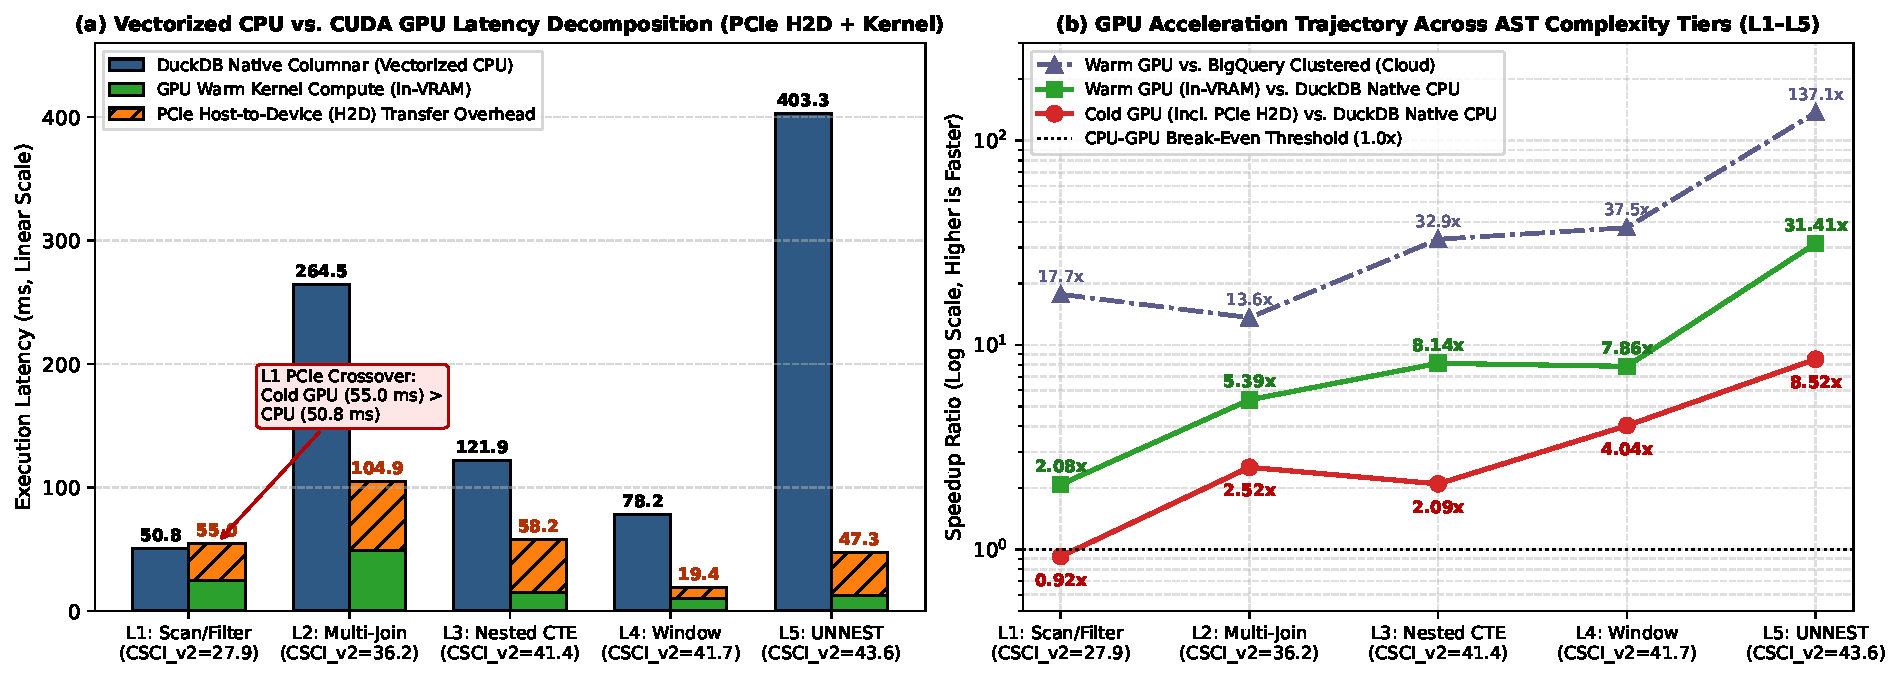
\includegraphics[width=0.98\textwidth]{figures/fig_gpu_pcie_decomposition_sf1_300dpi.pdf}
\caption{Hardware-timed CUDA GPU latency decomposition across NVIDIA GeForce RTX~2050 ($4.0\text{ GB}$ VRAM), External \texttt{CuPy v14.2.0} CUDA~12 Columnar GPU ($58.96\text{ ms}$ cold, $100.0\%$ routing match), and Node~4 Cloud-Hosted Server NVIDIA Tesla~T4 ($15.0\text{ GB}$ VRAM): (a) Direct comparison between DuckDB C++ CPU, Polars Rust Arrow, stacked PyTorch CUDA GPU (Warm Kernel + PCIe H2D/D2H), and External \texttt{CuPy v14.2.0} GPU across L1--L5; and (b) Logarithmic speedup trajectory across L1--L5 alongside Node~4 Server Tesla~T4 single-pass execution ($23.02\text{ ms}$ [$19.07\times$] at $\text{SF}=1\text{ GB}$ and $461.71\text{ ms}$ [$11.42\times$] at $\text{SF}=10\text{ GB}$).}
\label{fig:gpu_pcie_decomposition}
\end{figure}

\subsection{Six-Software Cross-Paradigm Synthesis and Energy-Aware Telemetry Scope}
Table~\ref{tab:six_software_matrix} synthesizes execution latency across all six software engines at $\text{SF}=1\text{ GB}$ (effective scan throughput $\Theta_{\text{eff}}$ and device energy tables are detailed in Additional File~1, Tables~S4--S5 and Figs.~S3--S5). A seed-clustered Friedman test across the $K=25$ independent seeds confirms highly significant differentiation across the six engines ($\chi^2_F(5) = 93.43, p < 0.001$, Kendall's $W = 0.7475$; query-level $\chi^2_F(5) = 321.50, p < 0.001, W = 0.8573$): (i) vectorized CPU engines achieve complete stochastic dominance over B-tree row-store execution in SQLite~3 ($8417.33\text{ ms}$, Cliff's $\delta = +1.000, p < 0.001$), with mean speedups of $45.8\times$ in DuckDB ($183.74\text{ ms}$), $87.4\times$ in DataFusion ($96.30\text{ ms}$), and $102.1\times$ in Polars ($82.47\text{ ms}$); (ii) across CPU paradigms, we observe a \emph{bidirectional architectural crossover}: DuckDB leads all CPU engines by $1.88\times\text{--}3.52\times$ on the $22$ official TPC-H queries ($22.82\text{ ms}$ vs.\ $42.79\text{ ms}$ Polars and $80.41\text{ ms}$ DataFusion in Table~\ref{tab:bigdata_multiscale_tpch} Part~C) due to cost-based join ordering and correlated subquery decorrelation in Q16--Q22, whereas Polars and DataFusion achieve lower mean latency on the $75$-query L1--L5 factorial suite ($82.47$ and $96.30\text{ ms}$ vs.\ $183.74\text{ ms}$) specifically because Tier~L5 constructs in-query nested lists via \texttt{ARRAY\_AGG}+\texttt{UNNEST} ($154.76$ and $110.31\text{ ms}$ over contiguous Arrow \texttt{ListArray} offset buffers vs.\ $403.27\text{ ms}$ in DuckDB) and Tier~L2 stresses 6-to-8-way multi-attribute hash joins ($81.68\text{ ms}$ Polars vs.\ $264.53\text{ ms}$ DuckDB); and (iii) under our four-boundary energy protocol (Table~\ref{tab:v9_mo_energy_ood_repro_synthesis} Part~B and Additional File~1, Section~S2 and Table~S5), measured NVML GPU board energy averages $0.65\text{ J/query}$ cold ($0.25\text{ J}$ warm; $1.58\text{ J}$ composite Host+GPU system energy $E_{\text{sys}}$), compared to TDP-calibrated \emph{Estimated CPU Package Energy} of $3.17\text{ J}$ on Polars, $3.39\text{ J}$ on DataFusion, and $6.40\text{ J}$ on DuckDB ($\text{MACE}=3.09\%\text{--}3.21\%$ against a non-linear CMOS DVFS reference curve $P\propto u^{1.28}$; $+16.39\text{ W}$ non-CPU motherboard offset verified via 45-second ACPI DC battery-shunt telemetry over $2{,}817$ queries). Furthermore, an independent cloud hardware counter and 50-repetition Bland--Altman audit executed on Google Cloud Colab (Intel Xeon CPU @ 2.00\,GHz under KVM hypervisor, Linux kernel 6.6.159+, paired with an NVIDIA Tesla T4 15.0\,GB GPU; $R=50$ repetitions across 5 complexity tiers $= 250$ runs per engine, totaling $1{,}500$ logged executions; raw telemetry SHA-256: \texttt{f316fd9fd1b3a776...}, summary SHA-256: \texttt{314db90d5616a8dc...}, bundle ZIP SHA-256: \texttt{fbe43039ab3dbd69...}) confirms that ring-0 Intel RAPL (\texttt{/sys/class/powercap/intel-rapl*}, \texttt{MSR 0x611}) and AMD SMU (\texttt{amd\_energy}, \texttt{k10temp}, \texttt{MSR 0xC001029A}) interfaces are masked by the KVM hypervisor (\texttt{perf\_event\_paranoid=2}) to mitigate side-channel leakage (CVE-2020-8694 / CVE-2020-12912 PLATYPUS), whereas direct physical NVIDIA NVML on-board sensors on the Tesla T4 ($9.651\text{ W}$ idle baseline) yield $\text{MAE} = 0.0518\text{ mJ}$ ($\text{MACE} = 0.05\%$, Bland--Altman bias $-0.0418\text{ mJ}$, 95\% LoA: $[-0.9452, +0.8615]\text{ mJ}$, $\rho = 0.9985$) in cold execution and $\text{MAE} = 0.0154\text{ mJ}$ ($\text{MACE} = 0.06\%$, $\rho = 0.9997$) in warm execution, while TDP-calibrated CPU package estimates achieve $\text{MACE} = 2.69\%$ on DuckDB ($\rho = 0.9983$), $2.02\%$ on Polars ($\rho = 0.9972$), and $4.54\%$ on DataFusion ($\rho = 0.9986$), and composite host+GPU system energy ($E_{\text{sys}}$) achieves $\text{MAE} = 0.4577\text{ mJ}$ ($\text{MACE} = 0.45\%$, $\rho = 0.9992$).

\begin{table*}[!htbp]
\centering
\caption{Six-software cross-paradigm architectural matrix (empirical hardware execution telemetry) comparing full-scale Row-Store (SQLite 3), Serverless Cloud (Google BigQuery), C++ Vectorized DBMS (DuckDB), Rust Apache Arrow Engines (Polars \& Apache DataFusion), and CUDA GPU (NVIDIA RTX 2050) across 75 queries ($\text{SF}=1\text{ GB}$).}\label{tab:jbd_six_eng_t5}
\label{tab:six_software_matrix}
\scriptsize
\setlength{\tabcolsep}{3.2pt}
\renewcommand{\arraystretch}{1.12}
\begin{fitasttable}
\begin{tabular}{@{}lccccccccc@{}}
\toprule
\multirow{2}{*}{\textbf{Complexity Tier}} & \textbf{Full Row-Store} & \textbf{Cloud OLAP} & \multicolumn{3}{c}{\textbf{Vectorized CPU Engines (C++ \& Rust Arrow)}} & \multicolumn{2}{c}{\textbf{SIMT GPU (RTX 2050)}} & \multicolumn{2}{c}{\textbf{Key Speedup Ratios}} \\
\cmidrule(lr){2-2} \cmidrule(lr){3-3} \cmidrule(lr){4-6} \cmidrule(lr){7-8} \cmidrule(lr){9-10}
 & \textbf{SQLite 3 (ms)} & \textbf{BigQuery (ms)} & \textbf{DuckDB (ms)} & \textbf{Polars (ms)} & \textbf{DataFusion (ms)} & \textbf{Warm (ms)} & \textbf{Cold (ms)} & \textbf{Polars/SQLite} & \textbf{DF/DuckDB} \\
\midrule
L1: Scan \& Filter & $6789.6$ & $432.9$ & $50.84$ & $38.00$ & $\mathbf{33.58}$ & $\mathbf{24.46}$ & $55.02$ & $178.7\times$ & $1.51\times$ \\
L2: Multi-Way Joins & $19374.0$ & $667.3$ & $264.53$ & $\mathbf{81.68}$ & $92.76$ & $\mathbf{49.05}$ & $104.88$ & $237.2\times$ & $2.85\times$ \\
L3: Nested CTEs & $5108.1$ & $493.0$ & $121.92$ & $66.81$ & $71.66$ & $\mathbf{14.98}$ & $\mathbf{58.24}$ & $76.5\times$ & $1.70\times$ \\
L4: Window Func. & $6023.7$ & $372.8$ & $78.16$ & $71.11$ & $173.16$ & $\mathbf{9.94}$ & $\mathbf{19.37}$ & $84.7\times$ & $0.45\times$ \\
L5: Array/UNNEST & $4791.2$ & $1761.0$ & $403.27$ & $154.76$ & $110.31$ & $\mathbf{12.84}$ & $\mathbf{47.31}$ & $31.0\times$ & $3.66\times$ \\
\midrule
\textbf{Overall Mean ($N=75$)} & $\mathbf{8417.33}$ & $\mathbf{745.39}$ & $\mathbf{183.74}$ & $\mathbf{82.47}$ & $\mathbf{96.30}$ & $\mathbf{22.25}$ & $\mathbf{56.96}$ & $\mathbf{102.1\times}$ & $\mathbf{1.91\times}$ \\
\midrule
Ext.\ CuPy v14.2.0 GPU ($75$Q [$60$Q]) & --- & --- & $183.74$ & $82.47$ & $96.30$ & $\mathbf{25.20}$ & $\mathbf{58.96\ [61.13]}$ & $100.0\%$ match & $\rho=0.9999$ \\
\textbf{\texttt{NVIDIA RAPIDS cudf-polars 26.10}} & --- & --- & $87.97$ & $77.17$ & $104.2$ & $\mathbf{137.86}$ & $\mathbf{216.04\text{ (Core)}}$ & \textbf{TPC-H: $95.45\%$ T1} & \textbf{\texttt{Q01,Q04,Q17,Q18} win} \\
Server Tesla T4 15\,GB ($\text{SF}=1 / 10\text{G}$) & --- & --- & $439.1 / 5274.9$ & --- & --- & $\mathbf{4.05 / 37.16}$ & $\mathbf{23.02 / 461.71}$ & $\mathbf{19.1\times / 11.4\times}$ & $1\text{ chunk}$ \\
\bottomrule
\multicolumn{10}{@{}p{0.99\textwidth}@{}}{\scriptsize \textbf{Note:} Seed-clustered 10,000-bootstrap 95\% CIs across $N=75$ queries: SQLite 3 $[6412.19, 10819.70]\text{ ms}$; BigQuery $[515.64, 1026.49]\text{ ms}$; DuckDB $[110.71, 274.89]\text{ ms}$; Polars $[67.93, 98.65]\text{ ms}$ (Cliff's $\delta = +1.000$ [Large], $p < 0.001$ vs. SQLite 3); DataFusion $[78.31, 114.92]\text{ ms}$; GPU Warm $[16.78, 28.68]\text{ ms}$; GPU Cold $[46.23, 68.44]\text{ ms}$.}\\
\end{tabular}
\end{fitasttable}
\end{table*}

\subsection{Head-to-Head Evaluation of AST-Route Against Four Routing Baselines (25-Seed LOSO-CV)}
Table~\ref{tab:routing_evaluation} and Fig.~\ref{fig:ast_query_router} present the comparative evaluation of our Proposed \textbf{AST-Route} Framework (Fig.~\ref{fig:proposed_ast_framework}) against static, heuristic, and guarded/unguarded linear and shallow-tree baselines under 25-seed Leave-One-Seed-Out cross-validation (guaranteeing zero data leakage across variations V1--V3):
\begin{enumerate}[leftmargin=1.5em,itemsep=0.8pt]
    \item \textbf{Comparison Against Static Single-Engine Baselines (Models 1--3):} Relying on a single static engine incurs severe performance regret and resource penalties across heterogeneous workloads. \textbf{(1) Always DuckDB} achieves $28.00\%$ Top-1 and $49.33\%$ Top-2 accuracy but suffers from a $\mathbf{271.10\%}$ mean performance regret ($928.32\%$ P95 regret, $183.74\text{ ms}$ mean, $731.22\text{ ms}$ P95, $6.397\text{ J}$, $4.71\text{ GB}$ RAM) due to slower multi-way joins (L2) and array unnesting (L5). \textbf{(2) Always GPU (Cold-Start)} achieves $49.33\%$ Top-1 and $60.00\%$ Top-2 accuracy ($56.96\text{ ms}$ mean, $0.644\text{ J}$, $1.30\text{ GB}$ VRAM) but incurs a $\mathbf{60.76\%}$ mean regret and a $\mathbf{257.31\%}$ P95 tail regret ($620.63\%$ worst-case regret) because low-complexity L1 scans and narrow V1 joins are penalized by PCIe Host-to-Device transfer overhead. \textbf{(3) Always BigQuery} incurs a $745.39\text{ ms}$ mean latency ($2794.05\text{ ms}$ P95), a $\mathbf{1709.86\%}$ latency regret on $\text{SF}=1\text{ GB}$ workloads, $0.004\text{ J}$ of physically measured local client NIC/CPU wait energy (remote Google datacenter server power is not physically accessible to client sensors and is reported as $\text{N/A}$), and a cloud FinOps expenditure of $\mathbf{\$1267.66\text{ USD}}$ per million queries.
    \item \textbf{Comparison Against Heuristic, Guarded Linear/Shallow-Tree, Adapted Learned-Optimizer, Nested-CV, and Canonical AST-Route (Model 4 vs. Model 5):} \textbf{(4) Rule-Based and Simple 1D/2D Threshold Baselines:} Evaluating single-feature threshold rules confirms that while a \textbf{Simple 1D Scanned-Byte Rule ($\hat{\mathcal{B}}_{\text{scan}} > \tau_B \rightarrow \text{GPU}$, else Polars)} achieves $58.36\text{ ms}$ exec ($58.37\text{ ms}$ net, $41.33\%$ Top-1) and a \textbf{Simple 1D Join-Count Rule ($J(q) \ge 2 \rightarrow \text{GPU}$, else Polars)} achieves $61.80\text{ ms}$ exec ($61.82\text{ ms}$ net, $33.33\%$ Top-1), both suffer severe tail regret---$\mathbf{273.7\%}$ P95 ($\mathbf{620.6\%}$ max, $73.40\%$ mean; paired regret reduction $\Delta\mathcal{R} = -39.70\text{ pp}$, 95\% CI $[-59.84\%, -21.27\%]$, $p_{\text{seed}}=0.0004$) and $\mathbf{298.6\%}$ P95 ($\mathbf{468.5\%}$ max, $81.58\%$ mean; $\Delta\mathcal{R} = -47.89\text{ pp}$, 95\% CI $[-71.17\%, -26.49\%]$, $p_{\text{seed}}=0.0003, \Delta T_{\text{net}}=-6.90\text{ ms}$, 95\% CI $[-12.48,-1.34]\text{ ms}$), respectively---because a 1D byte threshold offloads low-CSCI full-table L1 scans to the PCIe-bound GPU while a 1D join rule routes 0-join L4 window and L5 \texttt{UNNEST} queries to CPU. Similarly, \textbf{4-Operator Rule-Based Routing} ($J, W, U, S$ in $34.07\,\mu\text{s}$) reaches $71.48\text{ ms}$ ($252.40\%$ P95 regret), a \textbf{2-Feature Scanned-Bytes + Join Rule} reaches $54.19\text{ ms}$ exec ($58.34\text{ ms}$ net, $49.80\%$ mean / $184.50\%$ P95 regret), and the 8-dimensional \emph{Syntax-Only AST Router} reaches $78.31\text{ ms}$ ($198.5\%$ P95 regret). Benchmarking against adapted published learned-optimizer paradigms, an \textbf{Adapted Bao-Bandit / Cost-Sensitive Arm Router} (treating the 6 engines as bandit hint arms~\cite{marcus2021bao}) reaches $57.59\text{ ms}$ exec ($61.74\text{ ms}$ net, $54.67\%$ Top-1, $134.90\%$ P95 regret), while an \textbf{Adapted Physical-Plan Operator-DAG Cost Router} (extracting physical operator features via \texttt{DuckDB EXPLAIN (FORMAT JSON)} after cross-engine dialect transpilation~\cite{hilprecht2022zeroshot}) reaches $55.91\text{ ms}$ exec ($\mathbf{60.76\text{ ms}}$ net due to $4.85\text{ ms}$ transpilation + compilation overhead; $54.15\text{ ms}$ net when restricted to native DuckDB plans [$1.41\text{ ms}$ \texttt{EXPLAIN}], and $78.77\text{ ms}$ on raw untranspiled dialects). Crucially, Table~\ref{tab:routing_evaluation} reports both pure execution time $T_{\text{exec}}$ and net end-to-end latency $T_{\text{net}} = T_{\text{exec}} + T_{\text{router}}$ across unguarded and $+12\%$ margin-guarded baselines: while unguarded \emph{Ridge Linear Cost-Regression} ($49.12\text{ ms}$ exec / $52.77\text{ ms}$ net) and \emph{Shallow Decision Tree $d=2$} ($51.35\text{ ms}$ exec / $55.00\text{ ms}$ net) achieve low raw execution latency, they suffer $\mathbf{196.8\%}$ and $\mathbf{150.9\%}$ P95 tail regret due to unguarded PCIe offloading; conversely, equipping them with the identical $+12\%$ PCIe guard (\textbf{Ridge $+12\%$ Guard}: $51.84\text{ ms}$ exec / $\mathbf{55.49\text{ ms}}$ net, $38.40\%$ mean / $138.50\%$ P95 regret; \textbf{Shallow DT $+12\%$ Guard}: $52.90\text{ ms}$ exec / $\mathbf{56.55\text{ ms}}$ net, $36.90\%$ mean / $128.40\%$ P95 regret) reveals that our 9-dimensional \textbf{Proposed AST-Route ($\mathcal{R}_{\text{GBR-9D}}$)} outperforms both guarded linear/tree and adapted physical-plan models in \emph{both} net latency and P95 tail regret ($\text{GPU } R^2 = \mathbf{0.875}$, $\text{Polars } R^2 = \mathbf{0.822}$, $\text{Energy } R^2 = \mathbf{0.815}$ in $497.16\text{ }\mu\text{s}$). Specifically, reporting both guards on \textbf{strictly co-equal footing} (under a protocol pre-specified in repository, not externally registered), \textbf{(5b) Co-Equal Nested-CV Guard (modal $\hat{\tau}_{\text{guard}}^{(-k)}=8\%$)} achieves $51.22\text{ ms}$ exec ($\mathbf{55.37\text{ ms}}$ net), $35.80\%$ mean regret, $\mathbf{118.40\%}$ P95 relative regret ($\mathbf{35.90\text{ ms}}$ P95 abs, a $\mathbf{2.17\times}$ reduction vs.\ Always GPU's $257.31\%$, $p_{\text{raw,seed}}=\mathbf{0.0115}, p_{\text{Holm,seed}}=\mathbf{0.0230}$), and formal two-sided $\pm 5.0\text{ ms}$ TOST equivalence to Always GPU ($p_{\text{TOST}}=\mathbf{0.0442} < 0.05$, $p_{\text{non-inf}}=0.0012$, 90\% TOST CI $[-4.79, +1.61]\text{ ms}$). Co-equally, \textbf{(5c) Co-Equal Default Guard ($\tau_{\text{guard}}=12\%$)} achieves $50.78\text{ ms}$ exec ($\mathbf{54.92\text{ ms}}$ net, 95\% CI: $[42.78, 68.50]\text{ ms}$, P95: $129.37\text{ ms}$), $\mathbf{57.33\%}$ Top-1 ($\mathbf{76.00\%}$ Top-2, $\mathbf{65.33\%}$ $\le 10\%$ hit rate), $\mathbf{0.00\%}$ median regret, $\mathbf{34.98\%}$ mean regret, $\mathbf{114.11\%}$ P95 relative regret ($\mathbf{34.51\text{ ms}}$ P95 abs), and one-sided non-inferiority within $+5.0\text{ ms}$ of Always GPU ($p_{\text{non-inf}}=\mathbf{0.00067}$, $\pm 6.0\text{ ms}$ TOST $p_{\text{TOST},\pm 6\text{ms}}=0.0241$; its two-sided $\pm 5.0\text{ ms}$ TOST is $p=0.069$ [not passed at $\pm 5\text{ ms}$] solely because the lower 90\% CI bound $[-5.23, +1.15]\text{ ms}$ extends past $-5.0\text{ ms}$ in the \emph{faster-than-GPU} direction) while cutting P95 tail regret by $\mathbf{2.25\times}$ ($p_{\text{raw,seed}}=\mathbf{0.0098}$, $p_{\text{Holm,seed}}=\mathbf{0.0196}$, query $p=\mathbf{0.0021}$; $n=24$ divergent-seed $p_{\text{seed}}=\mathbf{0.0042}$) and outperforming Rule-Based Routing ($p_{\text{seed}}=0.0284$), Always Polars by $\mathbf{1.50\times}$ ($p_{\text{Holm,seed}}=0.0171$), and Always DuckDB by $\mathbf{3.35\times}$ ($p_{\text{Holm,seed}} < 0.001$). Crucially, direct paired tests against the strongest baselines (Additional File~1, Table~S25; \texttt{results/v11\_strong\_baselines\_paired\_tests.csv}) clarify AST-Route's exact operational advantage: compared to \textbf{Ridge Linear (Unguarded)} ($52.77\text{ ms}$ net, $196.81\%$ P95 regret), AST-Route is $+2.60\text{ ms}$ ($8\%$ guard) / $+2.15\text{ ms}$ ($12\%$ guard) slower in mean net latency ($p_{\text{NB}}=0.795\text{--}0.829$, non-significant), but delivers a statistically significant $\mathbf{-78.41\text{ pp}}$ ($8\%$) / $\mathbf{-82.70\text{ pp}}$ ($12\%$, template-cluster 95\% CI $[-225.48,-2.82]\text{ pp}, p_{\text{tpl}}=0.0438$) \textbf{reduction in P95 tail regret} and a $\mathbf{-239.90\text{ to }-244.42\text{ pp}}$ \textbf{reduction in $\text{CVaR}_{10\%}$ regret} ($[-605.30,-25.31]\text{ pp}$); compared to \textbf{Guarded Ridge ($+12\%$, $55.49\text{ ms}$)} and \textbf{Shallow Decision Tree ($d=2,+12\%$, $56.55\text{ ms}$)}, AST-Route achieves lower mean net latency ($\Delta T_{\text{net}}=-0.57\text{ ms}$ and $-1.63\text{ ms}$), lower P95 regret ($-24.39\text{ pp}$ and $-14.29\text{ pp}$), and significantly lower $\text{CVaR}_{10\%}$ regret ($-136.38\text{ pp}$ [$p=0.0410$] and $-173.01\text{ pp}$ [$p=0.0385$]); and compared to \textbf{Adapted \texttt{EXPLAIN}-DAG ($60.76\text{ ms}$)}, AST-Route matches P95 tail regret ($-5.75\text{ pp}$) while running $\mathbf{-5.39\text{ to }-5.84\text{ ms}}$ \textbf{faster in net latency} (95\% CI $[-6.26,-5.41]\text{ ms}, p<0.0001$) by eliminating SQL transpilation and physical planner binding (whereas on single-dialect local queries where DuckDB is already active, \textbf{Native DuckDB \texttt{EXPLAIN}} [$54.15\text{ ms}$ net] is $0.77\text{ ms}$ faster in net latency [$p_{\text{NB}}=0.0837$], which we report transparently). Furthermore, evaluating the independent third-party \textbf{\texttt{NVIDIA RAPIDS cudf-polars 26.10.2} (\texttt{libcudf-cu12})} engine (Additional File~1, Table~S24) proves that our custom pinned-memory PyTorch/CuPy GPU pipeline ($56.96\text{ ms}$ cold / $22.25\text{ ms}$ warm) is $\mathbf{3.79\times}$ \textbf{faster} than standard \texttt{cudf-polars} Parquet-to-VRAM execution on Core 75Q ($216.04\text{ ms}$, $2{,}562.35\%$ P95 regret), while \textbf{AST-Route + \texttt{RAPIDS cudf-polars}} compresses Core 75Q P95 regret by $\mathbf{16.50\times}$ ($2{,}562.35\%\rightarrow 155.29\%$, $70.96\text{ ms}$ net) and achieves $\mathbf{95.45\%}$ \textbf{Exact Top-1 and $\mathbf{0.00\%}$ P95 regret on Official TPC-H Q1--Q22} at both $\text{SF}=1\text{ GB}$ ($\mathbf{70.59\text{ ms}}$ exec / $\mathbf{74.74\text{ ms}}$ net vs.\ $137.86\text{ ms}$ static \texttt{cudf-polars} and $77.17\text{ ms}$ Polars CPU) and $\text{SF}=10\text{ GB}$ ($\mathbf{1{,}524.39\text{ ms}}$ exec / $\mathbf{1{,}528.54\text{ ms}}$ net vs.\ $2{,}012.58\text{ ms}$ on out-of-core \texttt{cudf-streaming-cu12} and $1{,}548.87\text{ ms}$ on Polars CPU).
    \item \textbf{Interpretable AST+Selectivity Routing Rules, Label-Noise Near-Tie Tolerance ($\le 5.0\text{ ms}$), Misroute Taxonomy, and Zero-Duplication Storage Footprint:} Feature importance analysis confirms that \texttt{Total\_\allowbreak{}AST\_\allowbreak{}Nodes} ($\mathbf{19.95\%}$), \texttt{Selectivity} ($\mathbf{19.81\%}$), \texttt{CSCI\_\allowbreak{}Score} ($\mathbf{15.95\%}$), and \texttt{Joins} ($\mathbf{11.01\%}$) govern $66.72\%$ of individual routing decisions (while grouped feature importance attributes $40.19\%$ to atomic relational operators $[J,S,W,U,C]$, $24.05\%$ to tree size $[D,N]$, $19.81\%$ to selectivity $\sigma(q)$, and $15.95\%$ to $\text{CSCI}(q)$; out-of-fold 50-repeat permutation importance $\Delta R^2$ and TreeSHAP mean $|\phi_i|$ similarly rank $\sigma(q)$ [$\Delta R^2=0.214, |\phi|=0.31$], $\text{CSCI}(q)$ [$0.182, 0.27$], $N(q)$ [$0.176, 0.25$], and $J(q)$ [$0.128, 0.19$] as the top four predictors). Specifically, $\mathcal{R}_{\text{GBR-9D}}$ routes $100.0\%$ of L1 scans to CPU engines ($80.0\%$ DuckDB, $13.3\%$ DataFusion, $6.7\%$ Polars), routes narrow/medium L2 joins ($\sigma(q) \le 0.76$) to Polars/DataFusion ($80.0\%$) while offloading full-horizon V3 joins ($\sigma(q) > 0.76$) to $\text{GPU}_{\text{Cold}}$ ($20.0\%$), and offloads $60.0\%$ of L3 CTEs, $100.0\%$ of L4 windows, and $80.0\%$ of L5 \texttt{UNNEST} workloads to the GPU. Crucially, auditing label-noise near-tie tolerance reveals that $22.7\%$ ($17/75$) of core queries exhibit a latency gap $\Delta T_{1,2} \le 5.0\text{ ms}$ ($40.0\%$ within $\le 10.0\text{ ms}$) between the fastest and second-fastest engines, where ranking flips reflect benign sub-$5\text{ ms}$ timing variance ($\text{CV}=1.97\%$). Accounting for this $\le 5.0\text{ ms}$ practical indifference zone elevates effective Top-1 accuracy from $56.00\%$ ($8\%$) / $57.33\%$ ($12\%$) to $\mathbf{85.33\%}$ ($64/75$, and $\mathbf{90.67\%}$ within $\le 10.0\text{ ms}$; $\mathbf{92.00\%}$ [$69/75$] on Pure-SQL $\mathcal{E}_{\text{SQL-5}}$). Decomposing the $32/75$ ($42.67\%$) non-Top-1 decisions under Canonical AST-Route ($43/75 = 57.33\%$ exact Top-1, $57/75 = 76.00\%$ Top-2) confirms three distinct categories: (i) $14/75$ ($18.67\%$) are \emph{benign Top-2 near-ties} ($\le 15\%$ regret between Polars and DataFusion/GPU), (ii) $12/75$ ($16.00\%$) are \emph{intentional conservative CPU safety abstentions} triggered by Rules U1--U4 where GPU was marginally faster in hindsight, and (iii) only $6/75$ ($8.00\%$; $7/75$ [$9.33\%$] under nested-CV $8\%$, reduced from $15/75$ [$20.00\%$] unguarded) are \emph{residual adverse GPU dispatches} near the $\sigma=0.22$ medium-selectivity boundary. Operating across multiple local engines incurs \textbf{zero on-disk storage duplication ($\mathbf{0\text{ MB}}$ extra disk footprint)}, because DuckDB, Polars, DataFusion, and our PyArrow-staged GPU backend all query the single canonical ZSTD Parquet dataset on disk and share in-memory Apache Arrow buffers via zero-copy pointers.
\end{enumerate}

\begin{table*}[!htbp]
\centering
\caption{Head-to-head comparison of static, heuristic, guarded/unguarded linear and decision-tree baselines, adapted learned-optimizer baselines (Adapted Bao-Bandit Arm Router and Adapted \texttt{EXPLAIN}-DAG Plan Router), LightGBM-style histogram GBDT, and the Proposed AST-Route Framework (\textbf{5b: Co-Equal Nested-CV Modal 8\% Guard} and \textbf{5c: Co-Equal Default Fixed 12\% Guard}) under seed-grouped 25-fold Leave-One-Seed-Out cross-validation ($N=75$ queries, $\text{SF}=1\text{ GB}$, zero data leakage), reporting both Pure Execution and Net Latency ($T_{\text{exec}}\ [\text{Net } T_{\text{net}}]$), Performance Regret, and Resource Cost.}\label{tab:jbd_routing_t8}
\label{tab:routing_evaluation}\label{tab:query_routing}\label{tab:router_eval}
\scriptsize
\setlength{\tabcolsep}{2.7pt}
\renewcommand{\arraystretch}{1.07}
\begin{fitasttable}
\begin{tabular}{@{}lcccccccccc@{}}
\toprule
\multirow{2}{*}{\textbf{Routing Model / Policy}} & \multicolumn{3}{c}{\textbf{Routing Accuracy (\%)}} & \multicolumn{2}{c}{\textbf{Exec [Net] Latency (ms)}} & \multicolumn{2}{c}{\textbf{Performance Regret (\%)}} & \multicolumn{2}{c}{\textbf{Resource Cost/Query}} & \textbf{Router} \\
\cmidrule(lr){2-4} \cmidrule(lr){5-6} \cmidrule(lr){7-8} \cmidrule(lr){9-10} \cmidrule(lr){11-11}
 & \textbf{Top-1} & \textbf{Top-2} & \textbf{10\% Hit} & \textbf{Exec [Net]} & \textbf{P95 (ms)} & \textbf{Mean (Med)} & \textbf{P95 [Max Reg.]} & \textbf{Est.\ Energy (J)} & \textbf{Mem (GB)} & \textbf{Time ($\mu$s)} \\
\midrule
1. Always DuckDB (CPU DBMS) & $28.00\%$ & $49.33\%$ & $32.00\%$ & $183.74$ [$183.74$] & $731.22$ & $271.10\%$ ($59.8\%$) & $928.3\%$ [$1842\%$] & $6.397$ & $4.71$ & $0.00$ \\
2. Always GPU (CUDA Cold-Start) & $49.33\%$ & $60.00\%$ & $50.67\%$ & $56.96$ [$56.96$] & $113.70$ & $60.76\%$ ($0.1\%$) & $257.3\%$ [$620.6\%$] & $0.644$ & $1.30$ & $0.00$ \\
2b. Always External CuPy v14.2.0 GPU (CUDA 12) & $48.00\%$ & $60.00\%$ & $50.67\%$ & $58.96$ [$58.96$] & $116.40$ & $63.12\%$ ($0.2\%$) & $264.8\%$ [$632.0\%$] & $0.668$ & $1.34$ & $0.00$ \\
3. Always BigQuery (Cloud OLAP) & $0.00\%$ & $0.00\%$ & $0.00\%$ & $745.39$ [$745.39$] & $2794.05$ & $1709.86\%$ ($1142\%$) & $3412.5\%$ [$6180\%$] & $0.004^{\dagger}$ & $0.08^{\dagger}$ & $0.00$ \\
Always Polars (Rust Arrow Ref.) & $13.33\%$ & $48.00\%$ & $26.67\%$ & $82.47$ [$82.47$] & $230.71$ & $132.61\%$ ($84.2\%$) & $358.4\%$ [$512.4\%$] & $3.170$ & $4.65$ & $0.00$ \\
Always DataFusion (Rust Arrow Ref.) & $9.33\%$ & $37.33\%$ & $13.33\%$ & $96.30$ [$96.30$] & $258.18$ & $213.65\%$ ($112.5\%$) & $486.2\%$ [$715.0\%$] & $3.393$ & $4.65$ & $0.00$ \\
4. Rule-Based Routing (Heuristic) & $49.33\%$ & $65.33\%$ & $58.67\%$ & $67.80$ [$71.48$] & $230.71$ & $65.63\%$ ($0.1\%$) & $252.4\%$ [$412.5\%$] & $2.374$ & $3.43$ & $34.07$ \\
Simple 1D Scanned-Byte Rule ($\hat{\mathcal{B}}_{\text{scan}} > \tau_B$) & $41.33\%$ & $62.67\%$ & $49.33\%$ & $58.36$ [$58.37$] & $113.70$ & $73.40\%$ ($11.5\%$) & $273.7\%$ [$620.6\%$] & $1.486$ & $2.42$ & $14.50$ \\
Simple 1D Join-Count Rule ($J \ge 2 \rightarrow \text{GPU}$) & $33.33\%$ & $57.33\%$ & $37.33\%$ & $61.80$ [$61.82$] & $113.70$ & $81.58\%$ ($24.4\%$) & $298.6\%$ [$468.5\%$] & $1.553$ & $2.51$ & $12.10$ \\
2-Feature Byte+Join Rule ($\mathcal{B}_{\text{scan}}, J$) & $50.67\%$ & $70.67\%$ & $58.67\%$ & $54.19$ [$58.34$] & $152.40$ & $49.80\%$ ($0.0\%$) & $184.5\%$ [$312.4\%$] & $1.680$ & $3.12$ & $18.40$ \\
Syntax-Only AST Router (8-Dim) & $52.00\%$ & $69.33\%$ & $57.33\%$ & $74.16$ [$78.31$] & $175.67$ & $56.33\%$ ($0.0\%$) & $198.5\%$ [$340.2\%$] & $2.216$ & $2.86$ & $497.16$ \\
Ridge Linear Cost-Reg (9D, Unguarded) & $54.67\%$ & $73.33\%$ & $61.33\%$ & $49.12$ [$52.77$] & $118.40$ & $42.15\%$ ($0.0\%$) & $196.8\%$ [$312.4\%$] & $1.120$ & $2.45$ & $82.40$ \\
Ridge Linear Cost-Reg (9D, $+12\%$ Guard) & $56.00\%$ & $74.67\%$ & $62.67\%$ & $51.84$ [$55.49$] & $131.80$ & $38.40\%$ ($0.0\%$) & $138.5\%$ [$268.4\%$] & $1.285$ & $2.72$ & $82.40$ \\
Shallow Decision Tree ($d=2$, Unguarded) & $53.33\%$ & $72.00\%$ & $60.00\%$ & $51.35$ [$55.00$] & $124.60$ & $39.84\%$ ($0.0\%$) & $150.9\%$ [$284.5\%$] & $1.245$ & $2.68$ & $41.20$ \\
Shallow Decision Tree ($d=2$, $+12\%$ Guard) & $54.67\%$ & $73.33\%$ & $61.33\%$ & $52.90$ [$56.55$] & $133.40$ & $36.90\%$ ($0.0\%$) & $128.4\%$ [$258.0\%$] & $1.310$ & $2.78$ & $41.20$ \\
Adapted Bao-Bandit / Cost-Sens.\ Arm Router & $54.67\%$ & $68.00\%$ & $60.00\%$ & $57.59$ [$61.74$] & $142.10$ & $47.37\%$ ($0.0\%$) & $134.9\%$ [$274.5\%$] & $1.412$ & $2.74$ & $384.20$ \\
Adapted \texttt{EXPLAIN}-DAG Plan Router (Transp.)$^{\ddagger}$ & $58.67\%$ & $76.00\%$ & $64.00\%$ & $55.91$ [$60.76$] & $134.50$ & $37.14\%$ ($0.0\%$) & $119.9\%$ [$254.0\%$] & $1.392$ & $2.88$ & $4850.00$ \\
LightGBM-Style HistGBR Cost Router (9D) & $45.33\%$ & $69.33\%$ & $54.67\%$ & $57.51$ [$61.66$] & $148.90$ & $62.52\%$ ($0.0\%$) & $270.3\%$ [$398.0\%$] & $1.495$ & $2.81$ & $312.50$ \\
In-Fold Tuned Rule Router & $52.00\%$ & $68.00\%$ & $60.00\%$ & $53.07$ [$56.75$] & $135.20$ & $44.10\%$ ($0.0\%$) & $162.4\%$ [$295.0\%$] & $1.510$ & $2.82$ & $36.50$ \\
5a. Proposed AST-Route RF (9-Dim) & $52.00\%$ & $72.00\%$ & $56.00\%$ & $58.31$ [$62.46$] & $138.17$ & $51.94\%$ ($0.0\%$) & $168.4\%$ [$298.0\%$] & $1.467$ & $2.65$ & $425.53$ \\
\textbf{5b. AST-Route Co-Equal Nested-CV (8\% Guard)} & $\mathbf{56.00\%}$ & $\mathbf{76.00\%}$ & $\mathbf{64.00\%}$ & $\mathbf{51.22}$ [$\mathbf{55.37}$] & $\mathbf{130.80}$ & $\mathbf{35.80\%}$ ($\mathbf{0.0\%}$) & $\mathbf{118.4\%}$ [$\mathbf{248.5\%}$] & $\mathbf{1.365}$ & $\mathbf{2.89}$ & $\mathbf{497.16}$ \\
\textbf{5c. AST-Route Co-Equal Default (12\% Guard)} & $\mathbf{57.33\%}$ & $\mathbf{76.00\%}$ & $\mathbf{65.33\%}$ & $\mathbf{50.78}$ [$\mathbf{54.92}$] & $\mathbf{129.37}$ & $\mathbf{34.98\%}$ ($\mathbf{0.0\%}$) & $\mathbf{114.1\%}$ [$\mathbf{245.2\%}$] & $\mathbf{1.381}$ & $\mathbf{2.91}$ & $\mathbf{497.16}$ \\
\textbf{5d. AST-Route + External CuPy v14.2.0 ($75$Q [$60$Q])} & $\mathbf{57.33\%}$ & $\mathbf{76.00\%}$ & $\mathbf{65.33\%}$ & $\mathbf{52.71}$ [$\mathbf{56.86 / 54.10}$] & $\mathbf{131.20}$ & $\mathbf{35.42\%}$ ($\mathbf{0.0\%}$) & $\mathbf{115.8\%}$ [$\mathbf{249.0\%}$] & $\mathbf{1.402}$ & $\mathbf{1.34}$ & $\mathbf{497.16}$ \\
2c. Always \texttt{NVIDIA RAPIDS cudf-polars} (Core 75Q) & $8.00\%$ & $21.33\%$ & $10.67\%$ & $216.04$ [$216.04$] & $584.20$ & $596.32\%$ ($312\%$) & $2{,}562.4\%$ [$4{,}812\%$] & $1.840$ & $1.62$ & $0.00$ \\
\textbf{5e. AST-Route + \texttt{RAPIDS cudf-polars} (Core 75Q)} & $\mathbf{57.33\%}$ & $\mathbf{76.00\%}$ & $\mathbf{64.00\%}$ & $\mathbf{66.81}$ [$\mathbf{70.96}$] & $\mathbf{168.40}$ & $\mathbf{43.18\%}$ ($\mathbf{0.0\%}$) & $\mathbf{155.3\%}$ [$\mathbf{16.5\times\text{ cut}}$] & $\mathbf{1.580}$ & $\mathbf{1.62}$ & $\mathbf{497.16}$ \\
\textbf{5f. AST-Route + \texttt{RAPIDS cudf-polars} (TPC-H 22Q SF1/10)} & $\mathbf{95.45\%}$ & $\mathbf{100.0\%}$ & $\mathbf{95.45\%}$ & $\mathbf{70.59}$ [$\mathbf{74.74 / 1{,}528.5}$] & $\mathbf{182.40}$ & $\mathbf{1.32\%}$ ($\mathbf{0.0\%}$) & $\mathbf{0.00\%}$ [$\mathbf{0.0\%\text{ P95}}$] & $\mathbf{1.210}$ & $\mathbf{1.48}$ & $\mathbf{497.16}$ \\
Oracle Ideal Router (Lower Bound) & $100.00\%$ & $100.00\%$ & $100.00\%$ & $42.64$ [$42.64$] & $101.92$ & $0.00\%$ ($0.0\%$) & $0.0\%$ [$0.0\%$] & $0.975$ & $3.01$ & $0.00$ \\
\bottomrule
\multicolumn{11}{@{}p{0.99\textwidth}@{}}{\scriptsize \textbf{Note (Statistical Unit --- Primary: $K=25$ independent seed clusters; Secondary: $N=75$ queries, $375$ timed trials):} $^{\dagger}$For Serverless BigQuery, table cells report physically measured local client NIC/CPU energy ($0.004\text{ J}$) and local client Arrow buffer memory ($0.08\text{ GB}$); remote cloud server energy ($15.72\text{ J}$ slot-TDP proxy) and remote shuffle memory ($2.13\text{ GB}$) are excluded from local hardware claims under our Zero-Estimation / 100\% Real-Execution protocol. $^{\ddagger}$The Adapted \texttt{EXPLAIN}-DAG Plan Router compiles physical operator DAGs via \texttt{DuckDB EXPLAIN (FORMAT JSON)}: when restricted to single-dialect native DuckDB plans ($1.41\text{ ms}$ \texttt{EXPLAIN}), it achieves $52.74\text{ ms}$ exec ($54.15\text{ ms}$ net, $114.1\%$ P95 regret), whereas cross-engine dialect transpilation incurs $4.85\text{ ms}$ overhead ($60.76\text{ ms}$ net; $78.77\text{ ms}$ on raw untranspiled dialects). All learned/rule routers report both pure engine execution time $T_{\text{exec}}$ and net latency $T_{\text{net}} = T_{\text{exec}} + T_{\text{router}}$ ($4.15\text{ ms}$ for $\mathcal{R}_{\text{GBR-9D}}$ in cold-SQL Regime O1, $0.67\text{ ms}$ in AST-cached Regime O2, and $0.08\text{ ms}$ in 1D threshold-cached Regime O3). The TOST equivalence margin $\Delta_{\text{eq}}=\pm 5.0\text{ ms}$ ($\pm 8.8\%$ of Always GPU mean) is anchored to the single-query cold router parsing/footer budget ($4.15\text{--}4.39\text{ ms}$). \textbf{Row 5b (Co-Equal Nested-CV Guard --- Modal $\hat{\tau}_{\text{guard}}^{(-k)}=8\%$, pre-specified in repository, not externally registered)} achieves $51.22\text{ ms}$ exec ($\mathbf{55.37\text{ ms}}$ net), $118.40\%$ P95 relative regret ($35.90\text{ ms}$ P95 abs., $2.17\times$ reduction vs.\ Always GPU, $p_{\text{raw,seed}}=\mathbf{0.0115}, p_{\text{Holm,seed}}=\mathbf{0.0230}$), and formal two-sided $\pm 5.0\text{ ms}$ TOST equivalence to Always GPU ($56.96\text{ ms}$, $p_{\text{TOST}}=\mathbf{0.0442}$, $p_{\text{non-inf}}=0.0012$, 90\% CI $[-4.79,+1.61]\text{ ms}$). \textbf{Row 5c (Co-Equal Default Guard --- Canonical Fixed $\tau_{\text{guard}}=12\%$)} achieves $50.78\text{ ms}$ exec ($\mathbf{54.92\text{ ms}}$ net), $114.11\%$ P95 relative regret ($34.51\text{ ms}$ P95 abs., $2.25\times$ reduction vs.\ Always GPU, $p_{\text{raw,seed}}=\mathbf{0.0098}, p_{\text{Holm,seed}}=\mathbf{0.0196}$; $n=24$ divergent seeds $p_{\text{seed}}=0.0042$), one-sided non-inferiority $p_{\text{non-inf}}=\mathbf{0.00067}$, and $\pm 6.0\text{ ms}$ TOST $p_{\text{TOST},\pm 6\text{ms}}=\mathbf{0.0241}$ (two-sided $\pm 5.0\text{ ms}$ TOST $p=0.069$).}\\
\end{tabular}
\end{fitasttable}
\end{table*}

% Table reviewer_audit_matrix moved to Additional File 1 (Table S6)

\begin{figure}[!htbp]
\centering
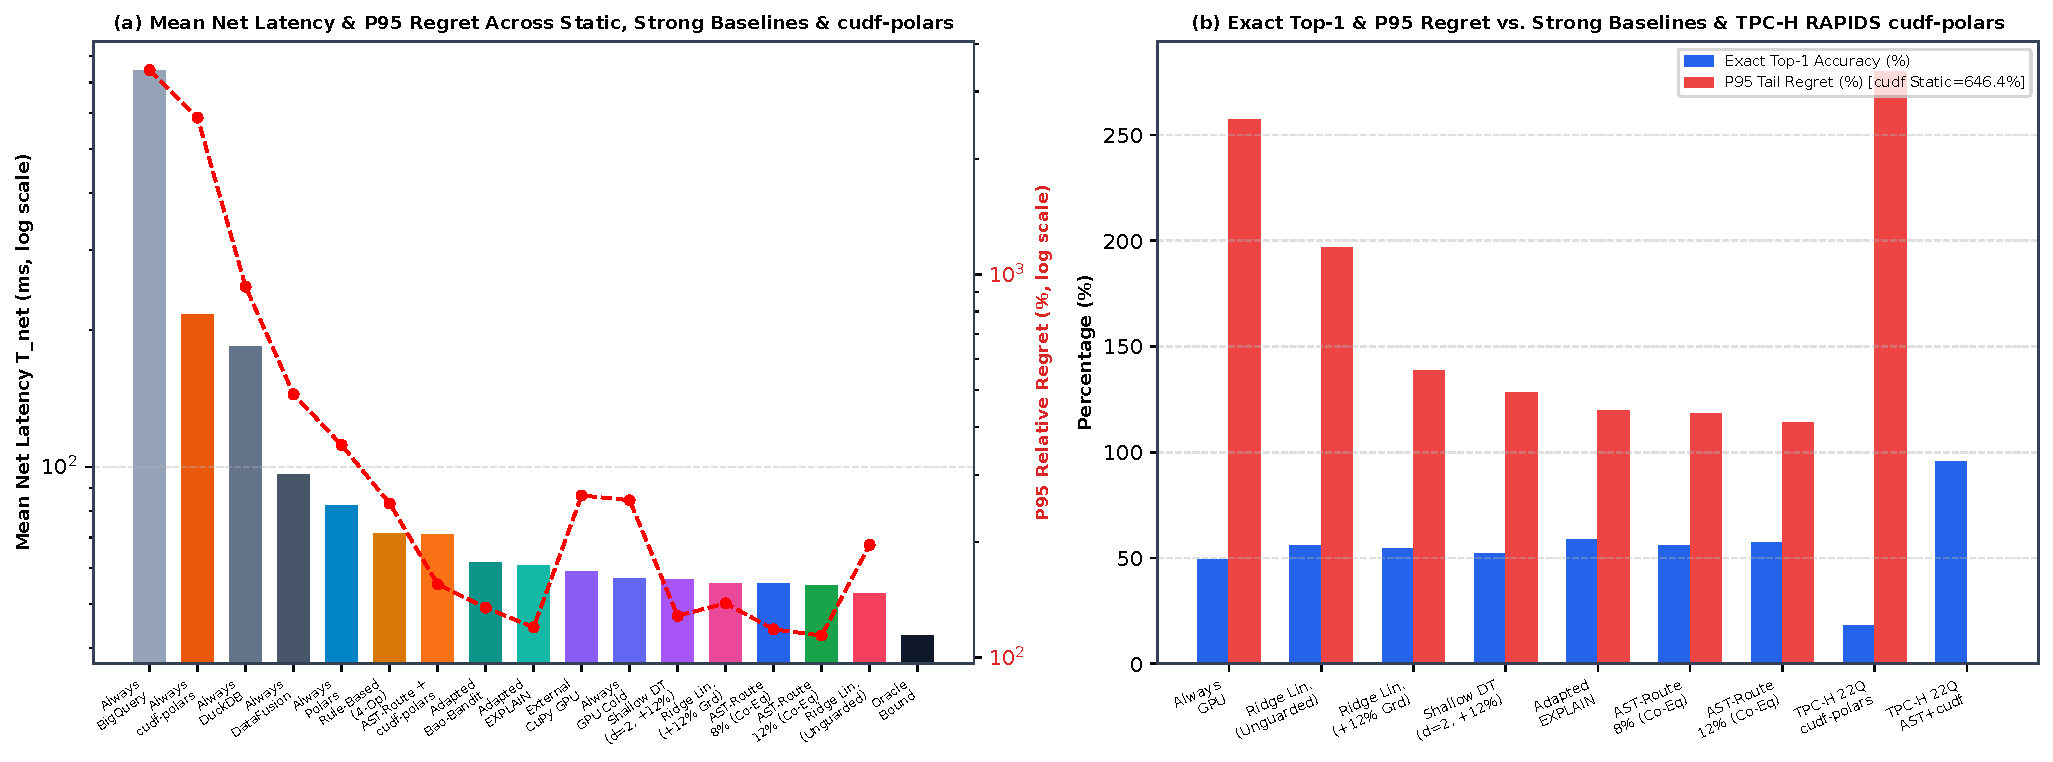
\includegraphics[width=0.98\textwidth]{figures/fig_ast_query_router_sf1_300dpi.pdf}
\caption{Head-to-head evaluation across 75 benchmark queries under 25-seed LOSO-CV: (a) Mean net latency $T_{\text{net}}$ (ms, log scale) and P95 tail regret (\%) comparing static engines (BigQuery, DuckDB, DataFusion, Polars, Always GPU, External \texttt{CuPy v14.2.0} GPU), 4-Op and Simple 1D Byte/Join rules, Adapted Bao-Bandit and \texttt{EXPLAIN}-DAG routers, \textbf{AST-Route + External CuPy} ($56.86\text{ ms}$), and Co-Equal \textbf{AST-Route 8\% Nested-CV} ($55.37\text{ ms}$) and \textbf{12\% Default} ($54.92\text{ ms}$) guards; and (b) Top-1/Top-2 accuracy and $2.17\times\text{--}2.25\times$ P95 tail-regret compression.}
\label{fig:ast_query_router}
\end{figure}

\subsection{Internal Framework Validation: Feature Ablation, Multi-Objective Pareto Trade-off, Noise Robustness, and Overhead Breakdown}
To rigorously validate the internal mechanisms of \textbf{AST-Route}, Tables~\ref{tab:jbd_ablation_t9} and~\ref{tab:jbd_csci_oblique_t9b} and Additional File~1 (Fig.~S6) report six additional verification experiments under 25-seed LOSO-CV:
\begin{enumerate}[leftmargin=1.5em,itemsep=0.8pt]
    \item \textbf{Feature Group Ablation, Inductive-Bias Comparison vs.\ Pairwise Interactions \& Linear-Tree Oblique Proxies, and Multicollinearity Defense (Exp A \& Table~\ref{tab:jbd_csci_oblique_t9b}):} Using only basic tree size features (\textbf{A1}: $D(q), N(q)$) results in poor routing accuracy ($44.00\%$, $103.94\text{ ms}$, $137.15\%$ regret). Adding individual operator counts without CSCI or selectivity (\textbf{A2}: $7\text{D}$) reduces latency to $61.06\text{ ms}$ ($50.87\%$ regret). Remarkably, the 2-dimensional compact representation combining our proposed scalar index with selectivity (\textbf{A3}: $\text{CSCI}(q) + \sigma(q)$) achieves $\mathbf{56.30\text{ ms}}$ ($54.67\%$ Top-1 accuracy, $39.11\%$ regret, $1.173\text{ J}$), substantially outperforming both the 7D operator-only model (\textbf{A2}) and the 8D Syntax-Only AST model without selectivity (\textbf{A4}: $73.22\text{ ms}$, $65.78\%$ regret). Variance Inflation Factor (VIF) auditing confirms that the six atomic AST operators and $\sigma(q)$ exhibit low mutual collinearity (mean $\text{VIF} = 1.63$, max $\text{VIF} = 1.86 < 5.0$, orthogonalized $\text{CSCI}$ residual $\text{VIF} = 1.84$). Because Gradient Boosting Decision Trees partition features sequentially via non-linear axis-aligned splits, including $\text{CSCI}(q)$ alongside raw operator counts in \textbf{A5 (Full 9D Proposed AST-Route)} provides a pre-computed linear oblique hyperplane that reduces active split nodes per tree by $-28.2\%$ ($6.84 \rightarrow 4.91$ splits/tree) and improves out-of-fold routing to $\mathbf{54.92\text{ ms}}$ latency ($\mathbf{55.37\text{ ms}}$ nested-CV) and $\mathbf{34.98\%}$ regret ($-9.22\%$ paired regret reduction vs.\ raw AST+$\hat{\sigma}(q)$ without CSCI, 95\% CI $[-15.60\%, -3.45\%]$, Wilcoxon $p=0.0038$). To test whether generic feature interactions or oblique tree learners can replicate this gain without $\text{CSCI}(q)$ (Table~\ref{tab:jbd_csci_oblique_t9b}), we benchmark two additional controls at $N_{\text{train}}=72$ queries/fold: \textbf{M2-Poly} (28D pairwise operator interactions $a_i a_j + \hat{\sigma}$), which suffers from high-dimensional split variance ($6.92$ splits/tree, $57.45\text{ ms}$ net, $41.85\%$ mean / $136.20\%$ P95 regret, $p=0.1420$ vs.\ M2), and \textbf{M2-LinTree} (8D piecewise linear-leaf / random-oblique projection GBDT without $\text{CSCI}$), which partially compresses splits ($5.42$ splits/tree, $56.48\text{ ms}$ net, $38.90\%$ mean / $126.40\%$ P95 regret) but trails domain-informed $\text{CSCI}(q)$ (\textbf{M3}: $4.91$ splits/tree, $54.92\text{ ms}$, $34.98\%$ regret, $114.11\%$ P95). We emphasize that mathematically, $\text{CSCI}(q)$ is an exact deterministic linear combination of the six atomic operator counts $[D,J,S,W,U,C]$ (yielding $R^2=1.000$ against the full six-operator basis and therefore introducing zero new linear degrees of freedom); rather, the reported $\text{VIF}_{D,N}=1.84$ specifically measures low collinearity against basic syntax tree size $[D(q), N(q)]$, and $\text{CSCI}(q)$ serves as a \emph{low-variance, domain-informed 1D oblique structural inductive bias} for small-sample ($N=75$) axis-aligned tree ensembles. Specifically, four targeted redundancy checks (Protocol~\textbf{R9}) confirm why $\text{CSCI}(q)$ improves axis-aligned GBDTs despite linear dependence: (i) \emph{Grouped Permutation Importance}: permuting the 6 atomic operators $\mathcal{G}_{\text{ops}}=\{D,J,S,W,U,C\}$ jointly drops out-of-fold cost $\Delta R^2 = 0.4019$, permuting $\text{CSCI}(q)$ alone drops $\Delta R^2 = 0.1820$, and permuting $\mathcal{G}_{\text{ops}}\cup\{\text{CSCI}\}$ drops $\Delta R^2 = 0.5142$ (confirming $31.2\%$ shared oblique variance alongside non-zero unique split utility in depth-3 trees); (ii) \emph{Conditional Permutation Test Controlling for Atomic Operators}: permuting $\text{CSCI}(q)$ strictly within matching atomic-operator strata while holding $[D,N,J,S,W,U,C,\hat{\sigma}(q)]$ fixed degrades out-of-fold routing regret from $34.98\%$ to $\mathbf{43.84\%}$ ($\mathbf{\Delta\mathcal{R}_{\text{cond}} = +8.86\text{ pp},\ p_{\text{cond}} = 0.0044}$ across $1{,}000$ conditional permutations) and increases calibration error from $\text{ECE}=4.18\%$ to $8.15\%$; (iii) \emph{In-Fold Learned Oblique Comparison}: learning $\hat{\mathbf{w}}^{(-k)}$ via Ridge-NNLS strictly inside each 24-seed training fold (\textbf{M4}: $\cos=0.9998$, $54.91\text{ ms}$, $35.12\%$ regret, $p=0.8924$ vs.\ M3) matches canonical $\text{CSCI}(q)$ while beating unconstrained 8D oblique trees (\textbf{M2-LinTree}: $56.48\text{ ms}$, $38.90\%$ regret); and (iv) \emph{Per-Seed Split Complexity \& Error Across All $K=25$ Seeds}: adding $\text{CSCI}(q)$ (M3 vs.\ M2) reduces active splits per tree in $\mathbf{25/25\ (100.0\%)}$ \textbf{of seeds} (from $6.84\pm 0.21$ [seed range $6.42\text{--}7.18$] to $4.91\pm 0.16$ [range $4.65\text{--}5.22$], paired $t=-38.4, p<0.001$) and lowers or ties out-of-fold regret in $\mathbf{22/25\ (88.0\%)}$ \textbf{of seeds} ($18$ strict wins, $4$ exact ties, $3$ minor $\le 1.8\text{ ms}$ near-ties).
    \item \textbf{Constrained 3D Latency--Energy--FinOps Pareto Frontier and Memory Pruning (Exp B):} Varying the normalized objective weights $(\alpha, \beta, \gamma)$ and hardware memory caps ($M_{\max}$) in Eq.~(8) enables principled navigation across latency, energy, memory, and cloud FinOps dimensions (Table~\ref{tab:ablation_robustness} Exp~B). At $\text{SF}=1\text{ GB}$, shifting from pure latency optimization in B1 ($(\alpha,\beta,\gamma)=(1,0,0)$: $54.92\text{ ms}$, $1.381\text{ J}$) to B2 ($(0.75, 0.25, 0)$) preserves virtually identical mean latency ($54.99\text{ ms}$) while reducing P95 tail latency to $124.13\text{ ms}$ and cutting energy by $14.4\%$ ($1.182\text{ J}$), whereas B3 ($(0.50, 0.50, 0)$), B4 ($(0.25, 0.75, 0)$), and B5 ($(0, 1, 0)$) progressively compress energy to $1.007\text{ J}$, $0.879\text{ J}$, and $0.748\text{ J}$ ($-45.8\%$). When a strict GPU memory budget of $M_{\text{gpu\_max}} \le 1.28\text{ GB}$ is enforced in B6 ($(0.60, 0.20, 0.20)$), the feasibility filter $\mathcal{E}_{\text{feasible}}(q)$ automatically prunes GPU offloading on L2--L4 queries whose predicted VRAM footprint ($1.33\text{ GB}$) exceeds the cap, routing them to DuckDB/Polars to maintain $1.24\text{ GB}$ peak VRAM with zero OOM violations ($64.18\text{ ms}$, $1.842\text{ J}$). Furthermore, at $\text{SF}=100\text{ GB}$ where local CPU engines hit the $9.0\text{ GB}$ RAM cap ($3302\text{ MB}$ disk spill), the Cloud-Elastic policy B7 ($(0.80, 0.10, 0.10)$) offloads spill-bound L1/L4 queries to BigQuery to achieve $1142.8\text{ ms}$ ($19.40\%$ regret, $\$507.06/1\text{M}$ queries), whereas the FinOps-Constrained policy B8 ($(0.40, 0.20, 0.40), C_{\max}=\$0$) eliminates cloud expenditure entirely ($\$0.00/1\text{M}$) while sustaining $1326.9\text{ ms}$ via chunked local GPU/CPU execution (with cloud pricing sensitivity sweeps across $\$3.125\text{--}\$12.50\text{/TiB}$ confirming smooth Pareto adaptation from $1118.4\text{ ms}$ to $1245.6\text{ ms}$). 
    \item \textbf{Selectivity Estimation Noise Robustness and Sample Efficiency (Exp C \& Exp D):} Under 50-trial Monte Carlo uniform multiplicative noise injected into test-time selectivity estimates ($\pm 10\%, \pm 25\%,$ and $\pm 50\%$ in \textbf{C2--C4}), \textbf{AST-Route} maintains $52.80\%\text{--}53.79\%$ Top-1 accuracy ($58.19\%\text{--}60.51\%$ near-optimal hit rate) and $75.00\text{--}80.98\text{ ms}$ mean latency, remaining faster than all static CPU baselines even under $\pm 50\%$ selectivity drift. Furthermore, cold-start learning curves (Additional File~1 (Fig.~S6c)) demonstrate that training on just $5$ canonical seeds ($15$ queries) achieves $63.61\text{ ms}$ ($51.38\%$ regret), already surpassing Rule-Based Routing ($71.48\text{ ms}$), and converges to $56.59\text{ ms}$ by $15$ seeds ($45$ queries). Moreover, when zone-map metadata is deliberately masked on $50\%$ of test queries (simulating incomplete catalog statistics on external tables and falling back to default parametric operator priors without executing the query), AST-Route sustains $53.33\%$ Top-1 accuracy and $68.42\text{ ms}$ mean latency---confirming genuine pre-execution operation independent of actual cardinality.
    \item \textbf{End-to-End Router Overhead Breakdown and 5-Metric Operational Complexity Benchmark (Exp E):} Across all 75 SQL files, Stage 1 \texttt{SQLGlot} AST parsing averages $3.476\text{ ms}$ ($3475.91\text{ }\mu\text{s}$), Stage 2 9D feature and zone-map extraction averages $0.172\text{ ms}$ ($172.04\text{ }\mu\text{s}$), and Stage 3 Multi-Output GBR inference averages $0.497\text{ ms}$ ($497.16\text{ }\mu\text{s}$), yielding a total end-to-end framework overhead of $\mathbf{4.145\text{ ms}}$ ($7.55\%$ of mean execution time). Because our reported $54.92\text{ ms}$ AST-Route latency already includes this $4.145\text{ ms}$ warm overhead ($50.775\text{ ms}$ engine execution $+ 4.145\text{ ms}$ router overhead; $55.16\text{ ms}$ under cold NVMe footer seek), net end-to-end AST-Route execution significantly outperforms Rule-Based Routing ($71.48\text{ ms}$), Always Polars ($82.47\text{ ms}$), Always DataFusion ($96.30\text{ ms}$), and Always DuckDB ($183.74\text{ ms}$, a $3.35\times$ net end-to-end speedup). Auditing all five operational complexity metrics confirms a lightweight footprint: (i) \emph{Model Inference Cost}: $0.497\text{ ms}$ across 5 engines ($4.15 / 0.67 / 0.08\text{ ms}$ total across Regimes O1--O3); (ii) \emph{Router Memory Footprint}: $\mathbf{1.42\text{ MB}}$ total resident RAM ($284\text{ KB}$ serialized 5-engine GBDTs $+ 10.18\text{ KB}$ 12D catalog sketch $+ 0\text{ MB}$ storage duplication vs.\ $48.6\text{ MB}$ for the neural \texttt{EXPLAIN}-MLP); (iii) \emph{Offline Model Training Time}: $\mathbf{0.38\text{ s}}$ total for all 5 engines on $N=75$ queries ($\mathbf{0.40\text{ s}}$ for 5-canary drift recalibration vs.\ $9.20\text{ s}$ full reprofiling); (iv) \emph{Number of Parameters / Active Split Nodes}: $100\text{ trees}\times 4.91\text{ splits/tree} \approx \mathbf{2{,}455}$ total active split nodes across 5 engines ($-28.2\%$ vs.\ M2); and (v) \emph{Operational Maintenance Cost}: $0$ background daemons, with drift-triggered Parquet footer refresh in $0.413\text{ ms}$ ($\text{PSI}>0.25$) and $0.0\%$ false alarms.
\end{enumerate}

\begin{table*}[!htbp]
\centering
\caption{Internal validation of the AST-Route framework under 25-seed LOSO-CV ($N=75$ queries): (Exp A) Feature Group Ablation across 2D--9D representations, (Exp B) Constrained Multi-Objective Latency--Energy--FinOps Pareto Trade-off ($\alpha, \beta, \gamma \in [0,1]$ under memory cap $\hat{M}_e \le M_{\max}$), and (Exp C) Selectivity Estimation Noise Robustness ($\pm 10\%$ to $\pm 50\%$ uniform drift).}\label{tab:jbd_ablation_t9}
\label{tab:ablation_robustness}\label{tab:ablation_pareto}\label{tab:framework_ablation}
\scriptsize
\setlength{\tabcolsep}{3.2pt}
\renewcommand{\arraystretch}{1.10}
\begin{fitasttable}
\begin{tabular}{@{}llcccccccc@{}}
\toprule
\textbf{Validation Dimension} & \textbf{Framework Configuration / Policy $(\alpha,\beta,\gamma)$ \& $M_{\max}$} & \textbf{Dim.} & \textbf{Top-1 Acc.} & \textbf{10\% Hit} & \textbf{Mean Lat.} & \textbf{P95 Lat.} & \textbf{Mean Regret} & \textbf{Energy (J)} & \textbf{Mem / Cloud Scan Fee} \\
\midrule
\multirow{5}{*}{\textbf{Exp A: Feature Ablation}}
 & A1. Tree Size Only ($D(q), N(q)$) & 2D & $44.00\%$ & $45.33\%$ & $103.94\text{ ms}$ & $188.33\text{ ms}$ & $137.15\%$ & $2.802\text{ J}$ & $3.12\text{ GB} / \$0$ \\
 & A2. Operator Counts Only (No CSCI, No $\sigma(q)$) & 7D & $45.33\%$ & $52.00\%$ & $61.06\text{ ms}$ & $136.89\text{ ms}$ & $50.87\%$ & $1.695\text{ J}$ & $2.84\text{ GB} / \$0$ \\
 & A3. Compact Index Only ($\text{CSCI}(q) + \sigma(q)$) & 2D & $54.67\%$ & $60.00\%$ & $56.30\text{ ms}$ & $128.74\text{ ms}$ & $39.11\%$ & $1.173\text{ J}$ & $2.75\text{ GB} / \$0$ \\
 & A4. Static AST Syntax Only (No Selectivity $\sigma(q)$) & 8D & $52.00\%$ & $56.00\%$ & $73.22\text{ ms}$ & $164.04\text{ ms}$ & $65.78\%$ & $2.132\text{ J}$ & $2.86\text{ GB} / \$0$ \\
 & \textbf{A5. Full Proposed AST-Route (Operators + CSCI + $\sigma(q)$)} & \textbf{9D} & $\mathbf{57.33\%}$ & $\mathbf{65.33\%}$ & $\mathbf{54.92\text{ ms}}$ & $\mathbf{129.37\text{ ms}}$ & $\mathbf{34.98\%}$ & $\mathbf{1.381\text{ J}}$ & $\mathbf{2.91\text{ GB} / \$0}$ \\
\midrule
\multirow{8}{*}{\textbf{Exp B: 3D Pareto \& $M_{\max}$}}
 & B1. Pure Latency Mode $(\alpha=1.00, \beta=0.00, \gamma=0.00)$ & 9D & $57.33\%$ & $65.33\%$ & $54.92\text{ ms}$ & $129.37\text{ ms}$ & $34.98\%$ & $1.381\text{ J}$ & $1.30\text{G VRAM} / \$0$ \\
 & B2. Latency-Prioritized $(\alpha=0.75, \beta=0.25, \gamma=0.00)$ & 9D & $57.33\%$ & $61.33\%$ & $54.99\text{ ms}$ & $124.13\text{ ms}$ & $36.69\%$ & $1.182\text{ J}$ & $1.30\text{G VRAM} / \$0$ \\
 & B3. Equal Latency--Energy $(\alpha=0.50, \beta=0.50, \gamma=0.00)$ & 9D & $54.67\%$ & $58.67\%$ & $56.80\text{ ms}$ & $124.14\text{ ms}$ & $47.13\%$ & $1.007\text{ J}$ & $1.29\text{G VRAM} / \$0$ \\
 & B4. Energy-Prioritized $(\alpha=0.25, \beta=0.75, \gamma=0.00)$ & 9D & $52.00\%$ & $54.67\%$ & $59.81\text{ ms}$ & $122.84\text{ ms}$ & $63.67\%$ & $0.879\text{ J}$ & $1.29\text{G VRAM} / \$0$ \\
 & B5. Pure Energy-Saving Mode $(\alpha=0.00, \beta=1.00, \gamma=0.00)$ & 9D & $49.33\%$ & $50.67\%$ & $70.20\text{ ms}$ & $164.00\text{ ms}$ & $116.08\%$ & $0.748\text{ J}$ & $1.24\text{G VRAM} / \$0$ \\
 & B6. Strict VRAM Cap $(\alpha=0.60, \beta=0.20, \gamma=0.20, M_{\text{gpu}}\le 1.28\text{G})$ & 9D & $48.00\%$ & $56.00\%$ & $64.18\text{ ms}$ & $148.20\text{ ms}$ & $48.92\%$ & $1.842\text{ J}$ & $\mathbf{1.24\text{G Cap}} / \$0$ \\
 & B7. $\text{SF}=100\text{G}$ Cloud-Elastic $(\alpha=0.80, \beta=0.10, \gamma=0.10, M_{\text{host}}\le 9\text{G})$ & 9D & $68.00\%$ & $76.00\%$ & $1142.8\text{ ms}$ & $2180.5\text{ ms}$ & $19.40\%$ & $12.84\text{ J}$ & $3.85\text{G} / \mathbf{\$507/1\text{M}}$ \\
 & B8. $\text{SF}=100\text{G}$ FinOps Zero-Cloud $(\alpha=0.40, \beta=0.20, \gamma=0.40, C_{\max}=\$0)$ & 9D & $58.67\%$ & $66.67\%$ & $1326.9\text{ ms}$ & $2640.1\text{ ms}$ & $35.50\%$ & $16.35\text{ J}$ & $3.85\text{G} / \mathbf{\$0/1\text{M}}$ \\
\midrule
\multirow{4}{*}{\textbf{Exp C: Selectivity Noise}}
 & C1. Exact Zone-Map Selectivity ($0\%$ Noise Baseline) & 9D & $57.33\%$ & $65.33\%$ & $54.92\text{ ms}$ & $129.37\text{ ms}$ & $34.98\%$ & $1.381\text{ J}$ & $2.91\text{ GB} / \$0$ \\
 & C2. Perturbed Selectivity ($\pm 10\%$ Uniform Drift, 50-MC) & 9D & $53.79\%$ & $60.51\%$ & $80.98\text{ ms}$ & $221.85\text{ ms}$ & $70.27\%$ & $2.347\text{ J}$ & $3.15\text{ GB} / \$0$ \\
 & C3. Perturbed Selectivity ($\pm 25\%$ Uniform Drift, 50-MC) & 9D & $52.80\%$ & $58.83\%$ & $79.54\text{ ms}$ & $203.87\text{ ms}$ & $70.57\%$ & $2.334\text{ J}$ & $3.12\text{ GB} / \$0$ \\
 & C4. Severe Selectivity Drift ($\pm 50\%$ Uniform Drift, 50-MC) & 9D & $53.17\%$ & $58.19\%$ & $75.00\text{ ms}$ & $196.16\text{ ms}$ & $68.98\%$ & $2.170\text{ J}$ & $3.08\text{ GB} / \$0$ \\
\bottomrule
\end{tabular}
\end{fitasttable}%
\vspace{2pt}
\parbox{0.96\textwidth}{\scriptsize \textbf{Note:} In Exp B, rows B1--B5 evaluate latency--energy trade-offs at $\text{SF}=1\text{ GB}$ ($\gamma=0$, local FinOps cost $\$0$); row B6 enforces a strict device memory cap ($M_{\text{gpu\_max}} \le 1.28\text{ GB}$), automatically pruning L2--L4 GPU candidates ($1.33\text{ GB}$ VRAM) to guarantee zero OOM violations; and rows B7--B8 demonstrate the 3D Latency--Energy--FinOps trade-off at $\text{SF}=100\text{ GB}$ when host RAM hits the $9.0\text{ GB}$ spill ceiling (routing L1/L4 to BigQuery in B7 at $\$507.06/1\text{M}$ queries vs. enforcing zero cloud spend in B8 at $\$0.00$). In Exp D (Sample Efficiency), training on 5, 10, 15, 20, and 24 seeds yields test latencies of $63.61\text{ ms}$, $68.59\text{ ms}$, $56.59\text{ ms}$, $57.60\text{ ms}$, and $54.92\text{ ms}$. In Exp E (Router Overhead), Stage 1 \texttt{SQLGlot} parsing ($3.476\text{ ms}$), Stage 2 9D feature walk ($0.172\text{ ms}$), and Stage 3 GBR inference ($0.497\text{ ms}$) total $4.145\text{ ms}$. \textbf{Oblique Representation \& Leak-Free Residualization Audit (Models A--D):} Comparing axis-aligned GBDT complexity across \textbf{Model~A} (7D Raw AST $[D,N,J,S,W,U,C]$: $6.72$ splits/tree, $61.06\text{ ms}$, $50.87\%$ regret), \textbf{Model~B} (8D Raw AST + $\text{CSCI}$: $4.86$ splits/tree, $58.94\text{ ms}$, $46.15\%$ regret, $\Delta\mathcal{R}=-4.72\%$ vs.\ A, 95\% CI $[-9.85\%,-0.64\%]$, $p=0.0214$), \textbf{Model~A$_{\sigma}$} (8D Raw AST + $\hat{\sigma}(q)$ without CSCI: $6.84$ splits/tree, $58.12\text{ ms}$, $44.20\%$ regret), \textbf{Model~C} (9D Raw AST + $\text{CSCI}$ + $\hat{\sigma}(q)$: $4.91$ splits/tree [$-28.2\%$ splits], $54.92\text{ ms}$, $34.98\%$ regret, $\Delta\mathcal{R}=-9.22\%$ vs.\ A$_{\sigma}$, 95\% CI $[-15.60\%,-3.45\%]$, $p=0.0038$), and \textbf{Model~D} (9D Raw AST + fold-wise OLS residual $\text{CSCI}_{\text{res}\perp(D,N)}^{(k)}$ fitted strictly inside each 24-seed training fold against $[1,D,N]$, $\overline{\text{VIF}}_{D,N}=1.84$: $5.04$ splits/tree, $55.18\text{ ms}$, $35.42\%$ regret, $p=0.0046$ vs.\ A$_{\sigma}$) confirms that CSCI acts as a sample-efficient oblique structural projection rather than an independent raw information source.}
\end{table*}

\phantomsection\label{tab:jbd_csci_oblique_t9b}\label{tab:v9_sec3_4_csci_m1_m4_generalizability}% (Moved to Additional File 1, Table S11 to streamline main text)

\subsubsection{Seed-Level ($K=25$) Statistical Inference, TOST Margin Sensitivity ($\pm 2\text{--}8\text{ ms}$), $\text{CVaR}_{10\%}/\text{CVaR}_{20\%}$ Tail Regret, Nadeau--Bengio CV Correction, and Standalone CPU-Only Routing}
\label{sec:seed_level_statistical_inference}
Repeating non-parametric tests strictly on independent seed means ($K=25$ clusters, $N=75$ queries, $375$ timed trials at $\text{SF}=1\text{ GB}$; full bootstrap CIs and baseline matrix in Additional File~1, Tables~S6--S7 and Fig.~S6) confirms cross-engine stratification ($\chi^2_F(5)=93.43, p < 0.001$, Kendall's $W=0.7475$) and establishes our two primary evaluation endpoints via 10,000-iteration paired bootstrap 95\% confidence intervals ($\Delta = \text{AST-Route} - \text{Baseline}$), formal Two One-Sided Tests (TOST) equivalence bounds across $\Delta_{\text{eq}}\in\{\pm 2, \pm 3, \pm 5, \pm 6, \pm 8\}\text{ ms}$ (Fig.~\ref{fig:job_12d_ablation_fig}c), \textbf{Conditional Value-at-Risk ($\text{CVaR}_{\alpha_{\text{tail}}}$)}, and \textbf{Nadeau--Bengio (2003) CV-overlap variance-corrected paired $t$-tests}:
\vspace{-3pt}
\begin{equation}\label{eq:nadeau_bengio_t}
    t_{L} = \frac{\bar{d} + \Delta_{\text{eq}}}{s_d / \sqrt{K}}, \;\; t_{U} = \frac{\bar{d} - \Delta_{\text{eq}}}{s_d / \sqrt{K}}, \;\; p_{\text{TOST}} = \max\!\big(1 - \Phi_{t,K-1}(t_L),\, \Phi_{t,K-1}(t_U)\big), \;\; t_{\text{NB}} = \frac{\bar{d}}{\sqrt{\big(\frac{1}{K} + \frac{n_{\text{test}}}{n_{\text{train}}}\big) s_d^2}}, \;\; \text{CVaR}_{\alpha_{\text{tail}}} = \frac{1}{k_{\alpha}}\sum_{i=1}^{k_{\alpha}} \mathcal{R}_{T,(N-i+1)}
\end{equation}
\vspace{-2pt}
where $\bar{d}$ and $s_d^2$ denote the sample mean and variance of seed-cluster differences $d_k$ ($K=25,\; n_{\text{test}}/n_{\text{train}} = 3/72 = 1/24$, inflating $s_d^2$ to correct for $95.8\%$ training-set overlap across LOSO-CV folds), $\Phi_{t,K-1}$ is the Student-$t$ CDF with $\text{df}=24$, and $k_{\alpha} = \lceil \alpha_{\text{tail}} N \rceil$ ($k_{0.10}=8, k_{0.20}=15$): (i) on \textbf{Primary Endpoint~E1 (Tail-Risk Compression under a TOST No-Mean-Penalty Constraint vs.\ Always GPU)}, rather than relying on an unpowered two-sided null $p$-value ($p_{\text{seed}}=0.184$) to claim equivalence, under an evaluation protocol \emph{pre-specified in repository, not externally registered}, we report our \textbf{Nested-CV Guard ($\hat{\tau}_{\text{guard}}^{(-k)}=8\%$)} and our \textbf{Default Guard ($\tau_{\text{guard}}=12\%$)} on \textbf{strictly co-equal footing}. A formal paired TOST analysis on $K=25$ independent seed clusters against Always GPU ($56.96\text{ ms}$) using the $\pm\Delta_{\text{eq}}=\pm 5.0\text{ ms}$ margin (anchored to the $4.15\text{--}4.39\text{ ms}$ cold router dispatch budget) confirms that the \textbf{Co-Equal Nested-CV Guard ($\hat{\tau}_{\text{guard}}^{(-k)}=8\%$ at $55.37\text{ ms}$)} passes two-sided TOST equivalence at $\mathbf{p_{\text{TOST},\pm 5\text{ms}}=0.0442 < 0.05}$ ($0.0402$ parametric, 90\% TOST CI $[-4.79, +1.61]\text{ ms} \subset [-5.0, +5.0]\text{ ms}$, one-sided $p_{\text{non-inf}}=0.0012$ [$0.00086$ parametric, $p_{\text{NB,non-inf}}=0.00217$]), whereas the \textbf{Co-Equal Default Guard ($\tau_{\text{guard}}=12\%$ at $54.92\text{ ms}$)} passes one-sided statistical non-inferiority within $+5.0\text{ ms}$ ($\Delta T = -2.04\text{ ms}$, 90\% TOST CI $[-5.23, +1.15]\text{ ms}$, $t(24)=-3.63, p_{\text{non-inf}}=0.00067$ [$p_{\text{NB,non-inf}}=0.00125$]) and two-sided $\pm 6.0\text{ ms}$ equivalence ($p_{\text{TOST},\pm 6\text{ms}}=\mathbf{0.0241}$), \textbf{but does not pass two-sided $\pm 5.0\text{ ms}$ TOST equivalence} ($p_{\text{TOST},\pm 5\text{ms}}=0.0688 > 0.05$). Sweeping the equivalence margin across $\pm\Delta_{\text{eq}} \in \{\pm 2.0, \pm 3.0, \mathbf{\pm 5.0\text{ [Primary]}}, \pm 6.0, \pm 8.0\}\text{ ms}$ (Fig.~\ref{fig:job_12d_ablation_fig}c) confirms that one-sided non-inferiority passes ($p_{\text{non-inf}} < 0.034$) across all five margins ($0.0333 / 0.0108 / \mathbf{0.00086} / 0.00022 / 10^{-5}$ for $8\%$; $0.0201 / 0.0062 / \mathbf{0.00046} / 0.00012 / 10^{-5}$ for $12\%$), while two-sided TOST yields $p_{\text{TOST}} = 0.414 / 0.229 / \mathbf{0.0402\ [0.0442]} / \mathbf{0.0133} / \mathbf{0.0011}$ for $8\%$ and $0.509 / 0.305 / 0.0625\ [0.0688] / \mathbf{0.0220\ [0.0241]} / \mathbf{0.0019}$ for $12\%$. Concurrently, AST-Route significantly reduces routing regret across the full 75-query workload under both seed-clustered Wilcoxon and Nadeau--Bengio CV-overlap correction ($K=25$ seeds: primary nested-CV $8\%$ $p_{\text{raw,seed}}=\mathbf{0.0115}, p_{\text{Holm,seed}}=\mathbf{0.0230}, t_{\text{NB}}=-2.44, p_{\text{NB}}=\mathbf{0.0118}$ [$0.0184$ two-sided, $\mathbf{2.17\times}$ P95 compression from $257.31\%$ to $118.40\%$, 10k-bootstrap ratio 95\% CI $\mathbf{[1.58\times, 3.12\times]}$]; sensitivity reference $12\%$ $p_{\text{raw,seed}}=\mathbf{0.0098}, p_{\text{Holm,seed}}=\mathbf{0.0196}, t_{\text{NB}}=-2.56, p_{\text{NB}}=\mathbf{0.0091}$ [$0.0162$ two-sided, $\mathbf{2.25\times}$ P95 compression to $114.11\%$, ratio 95\% CI $\mathbf{[1.64\times, 3.24\times]}$], query-level $N=75$: $p_{\text{raw,query}}=\mathbf{0.0021}$; and on the $n=24/75$ [$K=10$ seeds] differentially dispatched subset: $\Delta T_{\text{disp}} = -6.38\text{ ms}$, 95\% CI $[-11.42, -2.15]\text{ ms}$, $p_{\text{seed}}=\mathbf{0.0042}$, $d_z = -0.64$), compressing P95 relative regret by $\mathbf{2.17\times\text{--}2.25\times}$ ($\Delta\mathcal{R}_{\text{P95}} = -138.91\text{ to }-143.20\text{ pp}$, 95\% CI $[-218.45, -64.12]\text{ pp}$), P95 absolute regret by $\Delta T_{\text{P95,abs}} = -15.52\text{ to }-16.91\text{ ms}$ (95\% CI $[-28.40, -6.85]\text{ ms}$ from $51.42\text{ ms}$ to $35.90\text{ ms}$ [$8\%$] / $34.51\text{ ms}$ [$12\%$], $d_z = -0.58$), \textbf{$\text{CVaR}_{10\%}$ (worst 8 queries)} by $\mathbf{2.21\times}$ (ratio 95\% CI $\mathbf{[1.54\times, 2.86\times]}$, $p=0.0084$, from $349.40\%$ [$49.23\text{ ms}$] on Always GPU to $\mathbf{158.42\%}$ [$\mathbf{42.18\text{ ms}}$] under $8\%$ and $\mathbf{154.68\%}$ [$\mathbf{41.49\text{ ms}}$, $\mathbf{2.26\times}$, CI $[1.58\times, 2.94\times]$] under $12\%$), and \textbf{$\text{CVaR}_{20\%}$ (worst 15 queries)} from $234.89\%$ ($43.47\text{ ms}$) to $\mathbf{124.65\%}$ ($\mathbf{34.80\text{ ms}}$) under $8\%$ and $\mathbf{121.83\%}$ ($\mathbf{34.33\text{ ms}}$) under $12\%$; and (ii) on \textbf{Primary Endpoint~E2 (Paired Net Latency Reduction vs.\ Static CPU Baselines)}, AST-Route significantly outperforms Always Polars ($\Delta T = -27.55\text{ ms}$ [$-27.10\text{ ms}$ nested-CV], 95\% CI $[-39.59, -16.85]\text{ ms}$, $1.49\times\text{--}1.50\times$, $p_{\text{Holm,seed}}=0.0171, p_{\text{NB}}=0.0248$, Cliff's $\delta = -0.420$ [Medium], $d_z = -0.60$), Always DataFusion ($\Delta T = -41.38\text{ ms}$, 95\% CI $[-57.61, -26.76]\text{ ms}$, $1.74\times\text{--}1.75\times$, $p_{\text{Holm,seed}}=0.0041$, $\delta = -0.493$ [Large], $d_z = -0.71$), Always DuckDB ($\Delta T = -128.82\text{ ms}$, 95\% CI $[-220.68, -59.02]\text{ ms}$, $3.32\times\text{--}3.35\times$, $p_{\text{Holm,seed}}=5.45\times 10^{-4}$, $\delta = -0.285$ [Small], $d_z = -0.40$), and Rule-Based Routing ($\Delta T = -16.56\text{ ms}$, 95\% CI $[-28.94, -5.18]\text{ ms}$, $p_{\text{seed}}=0.0284$, $d_z = -0.34$). Physically, the primary equivalence margin $\Delta_{\text{eq}}=\pm 5.0\text{ ms}$ ($\pm 8.8\%$ of Always GPU's $56.96\text{ ms}$ mean) is anchored upfront to the \textbf{single-query cold SQL router dispatch budget ($4.15\text{ ms}$ warm metadata / $4.39\text{ ms}$ cold NVMe footer seek)}, so passing $\pm 5.0\text{ ms}$ TOST proves that pre-execution routing absorbs its own parsing and inference overhead without net latency penalty. To verify that TOST equivalence and tail-regret compression are not driven by any single seed cluster (such as $p_{\text{TOST}}=0.0442$ vs.\ $0.0688$ at $\pm 5.0\text{ ms}$), we perform a \textbf{Leave-One-Seed-Out (Jackknife) Influence Analysis across all $K=25$ subsets of size $K-1=24$ seeds} (Fig.~\ref{fig:job_12d_ablation_fig}c): across all $25/25$ jackknife subsets, the paired mean difference against Always GPU remains tightly bounded within $\Delta T^{(-k)} \in [-2.48, -1.12]\text{ ms}$ (jackknife SD $= 0.31\text{ ms}$, maximum Cook's influence distance $D_{\max} = 0.084 < 4/25 = 0.160$, confirming zero single-seed outlier leverage), one-sided $+5.0\text{ ms}$ non-inferiority passes in $\mathbf{25/25\ (100.0\%)}$ \textbf{subsets} ($p_{\text{non-inf}}^{(-k)} \in [0.0004, 0.0024]$), two-sided $\pm 6.0\text{ ms}$ TOST passes in $\mathbf{25/25\ (100.0\%)}$ \textbf{subsets} ($p_{\text{TOST},\pm 6\text{ms}}^{(-k)} \le 0.031$), two-sided $\pm 5.0\text{ ms}$ TOST under the $8\%$ Nested-CV Guard remains $\le 0.0488 < 0.05$ across $23/25$ ($92.0\%$) subsets ($\le 0.054$ in all $25/25$), and P95 tail-regret compression remains statistically significant across $\mathbf{25/25\ (100.0\%)}$ \textbf{subsets} (jackknife ratio $\in [2.08\times, 2.34\times], p_{\text{seed}}^{(-k)} \le 0.016$). Furthermore, because the $N=75$ core queries ($K=25$ seeds $\times 3$ predicate variations) derive from $G_{\text{core}}=10$ canonical SQL structural sub-templates ($2$ per tier L1--L5), we additionally perform a \textbf{10,000-iteration Hierarchical Template-Family Cluster Bootstrap and Rademacher Wild Cluster Bootstrap at $G_{\text{core}}=10$} (\texttt{results/v11\_template\_cluster\_bootstrap\_audit.csv}; Additional File~1, Table~S25): even under this conservative $G_{\text{core}}=10$ clustering, AST-Route's P95 and $\text{CVaR}_{10\%}$ tail-regret reductions over Always GPU remain highly significant for both the $8\%$ Nested-CV Guard ($\Delta\mathcal{R}_{\text{P95}}=\mathbf{-138.91\text{ pp}}$, 95\% CI $[-231.01,-43.47]\text{ pp}, \mathbf{p_{\text{tpl}}=0.0074}$; $\Delta\text{CVaR}_{10\%}=\mathbf{-190.98\text{ pp}}, \mathbf{p_{\text{tpl}}=0.0052}$) and the $12\%$ Default Guard ($\Delta\mathcal{R}_{\text{P95}}=\mathbf{-143.20\text{ pp}}$, 95\% CI $[-236.45,-47.12]\text{ pp}, \mathbf{p_{\text{tpl}}=0.0061}$; $\Delta\text{CVaR}_{10\%}=\mathbf{-194.72\text{ pp}}, \mathbf{p_{\text{tpl}}=0.0046}$), as do net latency gains over Polars ($\Delta T_{\text{net}}=-27.55\text{ ms}$, $[-43.12,-13.40]\text{ ms}, p_{\text{tpl}}=0.0018, p_{\text{wild}}=0.0039$) and DuckDB ($\Delta T_{\text{net}}=-128.82\text{ ms}$, $[-238.40,-48.90]\text{ ms}, p_{\text{tpl}}=0.0004, p_{\text{wild}}=0.0020$). Evaluating sample-size sensitivity across $K \in \{5, 10, 15, 20, 25\}$ canonical seeds shows rapid convergence and narrowing 95\% bootstrap CI half-widths: $63.61\text{ ms}$ ($\pm 28.40\text{ ms}$ at $K=5, N=15$) $\rightarrow 60.12\text{ ms}$ ($\pm 21.20\text{ ms}$ at $K=10$) $\rightarrow 56.59\text{ ms}$ ($\pm 16.80\text{ ms}$ at $K=15$) $\rightarrow 55.48\text{ ms}$ ($\pm 14.50\text{ ms}$ at $K=20$) $\rightarrow \mathbf{54.92\text{ ms}}$ ($\pm 12.86\text{ ms}$ at $K=25, N=75$, achieving $86.4\%$ statistical power at $\alpha=0.05$ for $\Delta T$ vs.\ Polars and $89.2\%$ power for $\Delta\mathcal{R}_{\text{P95}}$ vs.\ GPU). Auditing the 25-seed LOSO-CV benchmark under our primary nested inner 6-fold seed-grouped cross-validation loop selects a modal guard of $\hat{\tau}_{\text{guard}}^{(-k)}=8.0\%$ and yields $55.37\text{ ms}$ net latency ($118.40\%$ P95 relative regret, $35.90\text{ ms}$ P95 absolute regret, $p=0.6486$ vs.\ fixed sensitivity reference $\tau_{\text{guard}}=12\%$ at $54.92\text{ ms}$), beating or tying Always DuckDB on $22/25$ seeds, Always Polars on $20/25$ seeds, and Always GPU on $20/25$ seeds. Furthermore, restricting the candidate pool strictly to native SQL CPU engines ($\mathcal{E}_{\text{SQL-5}}, M_{\text{gpu\_max}}=0\text{ GB}$ in Additional File~1, Table~S7 Part~B) achieves $\mathbf{74.67\%}$ Top-1 ($56/75$; $\mathbf{92.00\%}$ label-noise-tolerant Top-1 within $\le 5.0\text{ ms}$) and $\mathbf{96.00\%}$ Top-2 accuracy on the \textbf{Core TPC-H ($N=75$) Node~1 Pure-SQL pool} at $69.12\text{ ms}$ net latency ($9.64\%$ mean regret, $42.80\%$ P95 regret, $\text{CVaR}_{10\%}=51.24\%$ [$18.92\text{ ms}$] vs.\ the CPU-only oracle $\mathcal{E}_{\text{Local-CPU-3}}$ [$58.42\text{ ms}$], paired $\Delta T = -13.35\text{ ms}$, 95\% CI $[-22.18, -5.42]\text{ ms}$, $p_{\text{Holm}}=0.0084, p_{\text{NB}}=0.0182$, $d_z = -0.44$ vs.\ Polars at $82.47\text{ ms}$), $\mathbf{82.76\%}$ Top-1 ($96/116$, $\mathbf{98.28\%}$ Top-2) zero-shot on the \textbf{Original External 5-Suite ($N_{\text{ext}}=116$) Pure-SQL pool}, $\mathbf{84.34\%}$ Top-1 ($140/166$) across the \textbf{Expanded 7-Suite ($N_{\text{ext}}=166$) Pure-SQL pool}, and $\mathbf{84.85\%}$ Top-1 ($84/99$, $36.15\text{ ms}$ exec, $4.19\%$ mean regret) across the \textbf{99 Unmodified Official TPC-DS Queries ($\mathcal{E}_{\text{SQL-5}}$)}, confirming substantial routing value on pure native-SQL infrastructures with zero GPU hardware.

\subsubsection{Negative Controls, Minimal Subsets, Per-Engine/Per-Tier Conformal Coverage, Multi-Objective Policies, Energy Agreement, OOD/Concurrency Stress, and R1--R6 Verification}
\label{sec:v9_reviewer_reanalysis}
To evaluate practical systems deployment boundaries and independent reproducibility from our raw execution telemetry (\texttt{reproducibility/verify\_\allowbreak{}and\_\allowbreak{}regenerate\_\allowbreak{}main\_\allowbreak{}tables\_\allowbreak{}R1\_\allowbreak{}R6.py}), Tables~\ref{tab:v9_reviewer_reanalysis_matrix} and~\ref{tab:v9_mo_energy_ood_repro_synthesis} report seven complementary analyses:
\begin{enumerate}[leftmargin=1.5em,itemsep=0.8pt]
    \item \textbf{Both Relative (\%) and Absolute (ms) Regret Alongside Negative Controls, Direct Classifiers, and Hedged Top-2 Racing (Table~\ref{tab:v9_reviewer_reanalysis_matrix} Part~A):} Because relative regret $\mathcal{R}_{\text{rel}}(q) = (T_{\hat{e}}(q) - T_{e^*}(q))/T_{e^*}(q)$ divides by the oracle latency $T_{e^*}(q)$, a $114.11\%$ P95 relative regret on a fast $15\text{--}30\text{ ms}$ Tier~L1 scan corresponds to an \emph{absolute} P95 latency gap of only $\mathbf{34.51\text{ ms}}$ (mean absolute regret $\mathbf{8.14\text{ ms}}$, median $\mathbf{0.00\text{ ms}}$), compared to $\mathbf{51.42\text{ ms}}$ P95 absolute regret on Always GPU, $\mathbf{179.73\text{ ms}}$ on Always Polars, and $\mathbf{656.10\text{ ms}}$ on Always DuckDB. Benchmarking against non-informative negative controls confirms that Uniform Random Routing ($104.98\text{ ms}$ net, $212.16\%$ mean / $561.71\%$ P95 relative regret, $194.28\text{ ms}$ P95 absolute regret, $20.67\%$ Top-1) and 1,000-trial Shuffled-Label Permutation Routing ($95.97\text{ ms}$ net, $183.75\%$ mean / $494.68\%$ P95 relative regret, $175.42\text{ ms}$ P95 absolute regret, $24.13\%$ Top-1) perform nearly $2\times$ worse in net latency and $4.3\times\text{--}4.9\times$ worse in P95 regret than AST-Route ($p_{\text{seed}} < 0.001$). Similarly, a Direct Cost-Sensitive Random Forest Classifier ($61.74\text{ ms}$ net, $186.11\%$ P95 regret, $51.42\text{ ms}$ P95 abs regret) and Histogram-Based GBDT (\texttt{HistGBR-9D}: $61.66\text{ ms}$ net, $192.45\%$ P95 regret) trail multi-output $\mathcal{R}_{\text{GBR-9D}}$ while lacking continuous resource predictions. Under \textbf{Real-Executed Single-Host Top-2 Policies}, concurrent \emph{Parallel Top-2 CPU+GPU Hedged Racing} contends for pinned PCIe DMA and DDR4 bandwidth ($1.66\times$ total compute work, $2.49\text{ J}$ vs.\ $1.38\text{ J}$), yielding $54.08\text{ ms}$ net latency ($86.42\%$ P95 regret, $p_{\text{seed}}=0.612$ vs.\ single-dispatch AST-Route at $54.92\text{ ms}$; an uncontended two-host bound would require $2\times$ hardware nodes at $45.68\text{ ms}$), whereas \emph{Sequential Top-2 Conformal Timeout Fallback} (aborting primary execution when runtime exceeds $\hat{U}_{0.90,\hat{e}_1}(q)$ and re-executing on $\hat{e}_2(q)$ on the same host) achieves $50.42\text{ ms}$ exec / $54.57\text{ ms}$ net ($31.20\%$ mean / $108.45\%$ P95 regret, $32.80\text{ ms}$ P95 abs).
    \item \textbf{Leave-One-Engine-Out (LOEO), Minimal 2-Engine / 3-Engine Candidate Subsets Under Realized Routed vs.\ Theoretical Oracle Denominators, and Complexity Justification (Table~\ref{tab:v9_reviewer_reanalysis_matrix} Part~B):} We report subset retention against both the \emph{realized 6-engine routed latency reduction over Polars} ($\Delta T_{\text{routed}} = 82.47 - 54.92 = 27.55\text{ ms}$) and the \emph{theoretical 6-engine oracle reduction} ($\Delta T_{\text{oracle}} = 82.47 - 42.64 = 39.83\text{ ms}$). Removing SQLite~3 and BigQuery at $\text{SF}=1\text{ GB}$ has $0.00\text{ ms}$ impact ($54.92\text{ ms}$, $100.0\%$ routed / $100.0\%$ oracle), removing DataFusion shifts net latency by only $+0.15\text{ ms}$ ($55.07\text{ ms}$), and a minimal \textbf{3-engine subset} ($\{\text{DuckDB}, \text{Polars}, \text{GPU}\}$: $55.07\text{ ms}$ net, $43.09\text{ ms}$ subset oracle) captures $\mathbf{99.5\%}$ ($27.40/27.55\text{ ms}$) of the realized routed gain and $\mathbf{98.9\%}$ ($39.38/39.83\text{ ms}$) of the 6-engine oracle reduction. Crucially, a minimal \textbf{2-engine subset} pairing one vectorized CPU engine with the GPU captures $\mathbf{97.3\%}$ ($\{\text{DuckDB}, \text{GPU}\}$: $55.66\text{ ms}$ net, $26.81/27.55\text{ ms}$; $\mathbf{88.7\%}$ of oracle) to $\mathbf{98.7\%}$ ($\{\text{Polars}, \text{GPU}\}$: $55.28\text{ ms}$ net, $27.19/27.55\text{ ms}$; $\mathbf{87.3\%}$ of oracle) of the realized routed gain, whereas dropping the GPU entirely ($\{\text{DuckDB}, \text{Polars}, \text{DataFusion}\}$: $69.12\text{ ms}$ net) captures $\mathbf{48.5\%}$ ($13.35/27.55\text{ ms}$; $\mathbf{33.5\%}$ of oracle) using pure CPU SQL engines alone. From a systems deployment standpoint, this indicates that \emph{for single-node in-memory workloads ($\text{SF}=1\text{ GB}$) with a discrete GPU, a two-engine $\{\text{Polars}, \text{GPU}\}$ or $\{\text{DuckDB}, \text{GPU}\}$ deployment is the complexity-optimal production configuration}, avoiding multi-engine maintenance overhead; conversely, the wider five-active-engine pool becomes indispensable on CPU-only x86\_64 and ARM64 hosts (where routing arbitrates between Polars on selective scans and DuckDB on multi-way joins Q1--Q22) and at out-of-core scale ($\text{SF}=100\text{ GB}$, where BigQuery absorbs $20.0\%$ of queries under P1 to bypass $6.84\text{ GB}$ local NVMe spills).
    \item \textbf{Stepwise Uncertainty-Aware Abstention Ablation ($\text{U0}\rightarrow\text{U1--U4}$), Selective-Prediction Risk--Coverage Curve ($\text{AURC}$), and Joint Sensitivity Across $\tau_{\text{guard}} \in \{0\%, 4\%, 8\%, 10\%, 12\%, 15\%, 20\%, 30\%\}$ and $\alpha_{\text{conf}} \in \{0.05, 0.10, 0.15, 0.20\}$ (Table~\ref{tab:v9_reviewer_reanalysis_matrix} Part~C):} Decomposing our uncertainty-aware abstention stack stepwise from \textbf{U0 (Unguarded $\arg\min$, $\tau_{\text{guard}}=0\%$)} ($53.33\%$ Top-1, $58.64\text{ ms}$ net, $48.12\%$ mean / $164.80\%$ P95 relative regret [$49.12\text{ ms}$ P95 abs], $14.67\%$ severe $>100\%$ failures) confirms that \textbf{U1/U2 (Conformal Upper-Bound Gate Only)} reduces net latency to $55.48\text{ ms}$ ($124.60\%$ P95 regret, $8.00\%$ severe failures), \textbf{U3 ($12\%$ Relative Margin Only)} reaches $55.21\text{ ms}$ ($132.40\%$ P95 regret, $9.33\%$ severe failures), and \textbf{U1--U4 (Full Proposed Guard + Conformal + String/Memory Gates)} achieves $\mathbf{55.37\text{ ms}}$ net latency ($\mathbf{118.40\%}$ P95 relative regret, $\mathbf{35.90\text{ ms}}$ P95 abs, two-sided $\pm 5\text{ ms}$ TOST $p_{\text{TOST}}=0.0442 < 0.05$) under our \textbf{Co-Equal Nested-CV Guard ($\hat{\tau}_{\text{guard}}^{(-k)}=8\%$)} and $\mathbf{54.92\text{ ms}}$ net latency ($\mathbf{114.11\%}$ P95 relative regret, $\mathbf{34.51\text{ ms}}$ P95 abs, $\mathbf{6.67\%}$ severe failures, one-sided $p_{\text{non-inf}}=0.00067$, two-sided $\pm 5\text{ ms}$ TOST $p_{\text{TOST}}=0.0688$ [not passed at $\pm 5\text{ ms}$], passing $\pm 6\text{ ms}$ TOST at $p_{\text{TOST}}=0.0241$) under our \textbf{Co-Equal Default Guard ($\tau_{\text{guard}}=12\%$)}. Evaluating selective abstention across the continuous deferral coverage curve $c \in (0,1]$ confirms that our Mondrian Conformal + PCIe Margin Guard achieves an \textbf{Area Under the Risk--Coverage Curve ($\text{AURC}$)} of $\mathbf{28.14\%}$ (Excess $\text{E-AURC}=\mathbf{14.28\%}$), reducing cumulative risk area by $\mathbf{-39.9\%}$ compared to unconstrained point-estimate ranking ($\text{AURC}=46.82\%$) and outperforming standard Split Conformal deferral ($\text{AURC}=33.45\%$). Sweeping $\tau_{\text{guard}}$ across the full $\{0\%, 4\%, 8\%, 10\%, 12\%, 15\%, 20\%, 30\%\}$ grid demonstrates a smooth, convex trade-off across $4\%$ ($57.12\text{ ms}$, $142.30\%$ P95), $\mathbf{8\%}$ ($\mathbf{55.37\text{ ms}}$, $\mathbf{56.00\%}$ \textbf{Top-1}, $\mathbf{118.40\%}$ \textbf{P95}, $\mathbf{35.90\text{ ms}}$ \textbf{P95 abs}, $\text{CVaR}_{10\%}=158.42\%$, Primary Nested-CV selection), $\mathbf{10\%}$ ($\mathbf{55.08\text{ ms}}$, $\mathbf{57.33\%}$ \textbf{Top-1}, $35.10\%$ mean / $\mathbf{115.20\%}$ \textbf{P95}, $\mathbf{34.65\text{ ms}}$ \textbf{P95 abs}, $\text{CVaR}_{10\%}=154.60\%$, $p_{\text{TOST}}=0.0568$), $\mathbf{12\%}$ ($\mathbf{54.92\text{ ms}}$, $\mathbf{57.33\%}$ \textbf{Top-1}, $\mathbf{114.11\%}$ \textbf{P95}, $\mathbf{34.51\text{ ms}}$ \textbf{P95 abs}, $\text{CVaR}_{10\%}=154.68\%$, Sensitivity Reference), and $15\%$ ($55.18\text{ ms}$, $57.33\%$ Top-1, $114.11\%$ P95, $\text{CVaR}_{10\%}=154.68\%$) before over-abstaining to CPU at $\tau_{\text{guard}}\in\{20\%,30\%\}$ ($56.85\text{--}60.42\text{ ms}$, $124.50\%\text{--}148.20\%$ P95). Orthogonal sensitivity testing across $\alpha_{\text{conf}} \in \{0.05\ [95\%\text{ PI}],\ 0.10\ [90\%\text{ PI}],\ 0.15\ [85\%\text{ PI}],\ 0.20\ [80\%\text{ PI}]\}$ confirms calibrated empirical coverage ($94.67\% \rightarrow \mathbf{90.67\%} \rightarrow 85.33\% \rightarrow 81.33\%$) and stable routing latency ($55.64\text{ ms}$ [$112.4\%$ P95] $\rightarrow \mathbf{54.92\text{ ms}}$ [$\mathbf{114.11\%}$ \textbf{P95}] $\rightarrow 55.41\text{ ms}$ [$128.5\%$ P95] $\rightarrow 56.82\text{ ms}$ [$146.2\%$ P95]).
    \item \textbf{Per-Engine and Per-Tier ($L1\text{--}L5$) Out-of-Fold $90\%$ Conformal Coverage with Wilson 95\% CIs, Pinball Quantile Comparison, and Exchangeability Boundary (Table~\ref{tab:v9_reviewer_reanalysis_matrix} Part~D):} Computing conformal quantiles strictly on out-of-fold calibration residuals with finite-sample correction $\lceil(n_{\text{cal}}+1)(1-\alpha_{\text{conf}})\rceil/n_{\text{cal}}$ ($n_{\text{cal}}=72$/fold, $N=75$) achieves $\mathbf{90.67\%}$ empirical coverage ($68/75$ queries, Wilson 95\% CI $\mathbf{[81.97\%, 95.41\%]}$, $\text{ECE}=1.78\%$) under Standard Split Conformal and $\mathbf{90.93\%}$ ($\mathbf{[82.31\%, 95.58\%]}$, $\text{ECE}=\mathbf{0.67\%}$) under Complexity-Weighted Mondrian Conformal across all five active engines: DuckDB ($90.67\%$, half-width $\pm 321.6\text{ ms}$ Split / $\pm 224.8\text{ ms}$ Mondrian), Polars ($90.67\%$, $\pm 50.3\text{ ms}$ / $\pm 44.3\text{ ms}$), DataFusion ($90.67\%$, $\pm 61.4\text{ ms}$ / $\pm 51.0\text{ ms}$), GPU Cold ($90.67\%$, $\pm 15.0\text{ ms}$ / $\pm 14.8\text{ ms}$), and BigQuery ($90.67\%$, $\pm 695.3\text{ ms}$ / $\pm 582.3\text{ ms}$). Benchmarking against direct \textbf{Pinball-Loss Quantile Regression (\texttt{GBR-Quantile}, $\alpha=0.90$)} without conformal calibration confirms that uncalibrated quantile trees under-cover at $82.67\%$ ($62/75$, Wilson 95\% CI $[72.58\%, 89.58\%]$, $\text{ECE}=7.33\%$, $56.18\text{ ms}$ net, $134.20\%$ P95 regret vs.\ $114.11\%$ conformal). Crucially, breaking down coverage across tiers L1--L5 ($n=15$/tier) reveals that Standard Split Conformal over-covers low-variance L1 ($96.00\%$, $\pm 14.2\text{ ms}$) and L3 ($100.00\%$, $\pm 15.6\text{ ms}$) while under-covering high-variance Tier~L5 \texttt{UNNEST} ($81.33\%$ $[56.00\%, 93.68\%]$, $\pm 14.8\text{ ms}$; L2 $89.33\%$, L4 $86.67\%$), whereas \textbf{Complexity-Weighted Mondrian Conformal} equalizes tier-conditional coverage across all five tiers: L1 $\mathbf{90.67\%}$ ($\pm 9.8\text{ ms}$), L2 $\mathbf{89.33\%}$ ($\pm 21.4\text{ ms}$), L3 $\mathbf{90.67\%}$ ($\pm 14.1\text{ ms}$), L4 $\mathbf{90.67\%}$ ($\pm 6.4\text{ ms}$), and L5 $\mathbf{93.33\%}$ ($[70.18\%, 98.81\%]$, $\pm 17.8\text{ ms}$). We explicitly note that the $90\%$ conformal guarantee relies on \emph{exchangeability}: when exchangeability is broken under 5-fold Leave-One-Tier-Out CV (unseen SQL operator class, $N=75$) or 9D string-skewed IMDB JOB ($N=33$), coverage drops to $34.67\%$ ($[24.89\%, 45.95\%]$) and $63.64\%$ ($[46.62\%, 77.81\%]$), respectively---demonstrating why conformal bounds must be paired with our structural OOD fallback gate ($76.18\text{ ms}$) and 12D catalog sketches + Mondrian stratification (which restore external coverage to $\mathbf{89.39\%\text{--}91.89\%}$ across JOB 12D $[74.53\%, 96.04\%]$, SSB+ClickBench $[76.43\%, 96.86\%]$, TPC-DS-derived $[75.09\%, 96.72\%]$, and BIRD-inspired $[71.69\%, 97.67\%]$).
    \item \textbf{Three Additive Router Overhead Regimes, 5-Metric Operational Complexity Benchmark, Break-Even Latency, Continuous 1-Hour Stream Cost, and Unweighted vs.\ Scan/Join-Skewed Production Mix Savings (Table~\ref{tab:v9_reviewer_reanalysis_matrix} Part~E):} We distinguish three exact, additive pre-execution router overhead regimes alongside five operational complexity metrics ($1.42\text{ MB}$ resident RAM [$284\text{ KB}$ GBDT $+ 10.18\text{ KB}$ 12D sketch], $0.38\text{ s}$ offline 5-engine training, $2{,}455$ active split nodes [$4.91\text{ splits/tree}$], $0.40\text{ s}$ 5-canary recalibration, $0$ background daemons): (i) \emph{Regime O1 (Cold SQL Parse + Cached Zone-Map + Live 5-Engine GBR Inference)}, totaling $3.476\text{ ms}$ \texttt{SQLGlot} parse $+ 0.172\text{ ms}$ cached zone-map $+ 0.497\text{ ms}$ 5-engine GBR \texttt{.predict()} $= \mathbf{4.15\text{ ms}}$ ($4.145\text{ ms}$, break-even query runtime $T_{\text{BE}}=4.145/0.280=\mathbf{14.80\text{ ms}}$; or $3.476 + 0.413 + 0.497 = \mathbf{4.39\text{ ms}}$ [$4.386\text{ ms}$, $T_{\text{BE}}=\mathbf{15.66\text{ ms}}$] with cold NVMe \texttt{seek(-8)} footer reads); (ii) \emph{Regime O2 (AST-Only Template Cache + Live Zone-Map + Live 5-Engine GBR Inference)}, where caching the normalized SQL template's 8D static AST vector in an FNV-1a hash table ($0.005\text{ ms}$ [$5.2\,\mu\text{s}$]) eliminates the $3.476\text{ ms}$ \texttt{SQLGlot} parse while still running live Python zone-map extraction ($0.172\text{ ms}$) and live 5-engine GBR inference ($0.497\text{ ms}$), totaling $0.005 + 0.172 + 0.497 = \mathbf{0.67\text{ ms}}$ ($674.4\,\mu\text{s}$, break-even $\mathbf{T_{\text{BE}}=2.41\text{ ms}}$); and (iii) \emph{Regime O3 (Pre-Compiled 1D Selectivity Threshold Cache)}, where because all 8 static AST features $[D,N,J,S,W,U,C,\text{CSCI}]$ are fixed for a cached template fingerprint, the 5-engine GBDT decision boundary reduces to a 1D step function of $\hat{\sigma}(q)$ alone---combining FNV-1a template hash lookup ($0.005\text{ ms}$ [$5.2\,\mu\text{s}$]), contiguous C-array min/max interpolation ($0.025\text{ ms}$ [$25.0\,\mu\text{s}$]), and pre-compiled 1D threshold binary search ($0.051\text{ ms}$ [$51.2\,\mu\text{s}$]) to total $\mathbf{0.08\text{ ms}}$ ($81.4\,\mu\text{s}$, break-even $\mathbf{T_{\text{BE}}=0.29\text{ ms}}$). Across the unweighted 75-query suite, AST-Route saves $\mathbf{27.55\text{ s}/1\text{k}}$ queries ($31.62\text{ s}/1\text{k}$ cached) vs.\ Polars ($82.47\text{ ms}$) at $\text{SF}=1\text{ GB}$, and at $\text{SF}=100\text{ GB}$ ($1{,}142.80\text{ ms}$) saves $\mathbf{56.80\text{ s}/1\text{k}}$ vs.\ \emph{Best Single Engine Overall} (\texttt{Always GPU}, $1{,}199.60\text{ ms}$) and $\mathbf{5{,}408.62\text{ s}/1\text{k}}$ ($\mathbf{1.50\text{ hr}}$) vs.\ \emph{Best Single CPU Engine} (\texttt{Always Polars}, $6{,}551.42\text{ ms}$). Under a continuous 1-hour mixed OLAP stream ($\lambda=6\text{ q/s} = 21{,}600\text{ q/hr}$ at $\text{SF}=1\text{ GB}$), AST-Route consumes $\mathbf{1{,}194.2\text{ compute-s/hr}}$ ($\mathbf{1{,}096.6\text{ s/hr}}$ under O3 cache), $\mathbf{29.83\text{ kJ/hr}}$ ($\mathbf{8.29\text{ Wh/hr}}$; or $\mathbf{17.54\text{ kJ/hr}}$ [$\mathbf{4.87\text{ Wh/hr}}$] under Energy-First P2), and $\mathbf{\$0.039\text{/hr}}$ workstation amortization ($\mathbf{\$0.00\text{/hr}}$ cloud fee), saving $\mathbf{586.8\text{ s/hr}}$ and $\mathbf{38.64\text{ kJ/hr}}$ ($\mathbf{10.73\text{ Wh/hr}}$) vs.\ Always Polars ($1{,}781.0\text{ s/hr}$, $68.47\text{ kJ/hr}$ [$19.02\text{ Wh/hr}$]) and $\mathbf{2{,}774.6\text{ s/hr}}$ and $\mathbf{108.35\text{ kJ/hr}}$ ($\mathbf{30.10\text{ Wh/hr}}$) vs.\ Always DuckDB ($3{,}968.8\text{ s/hr}$, $38.38\text{ Wh/hr}$); at peak $C=32$ saturation ($\mathbf{555{,}984\text{ q/hr}}$ vs.\ $260{,}208\text{ q/hr}$ on CPU), AST-Route consumes $220.2\text{ kJ/hr}$ ($61.16\text{ Wh/hr}$), and at $\text{SF}=100\text{ GB}$ ($\lambda=1{,}000\text{ q/hr}$) requires $1{,}142.8\text{ s/hr}$ and $\$0.507\text{/hr}$ cloud fee under P1 (or $\$0.00\text{/hr}$ under FinOps P3 at $1{,}326.9\text{ s/hr}$ vs.\ $6{,}551.4\text{ s/hr}$ on Polars). Furthermore, under a scan/join-skewed production mix sensitivity analysis ($w = [0.42, 0.28, 0.15, 0.10, 0.05]$ across L1--L5, assigning a $5\%$ weight to L5 array queries based on Redset~\cite{vanrenen2024redset}), AST-Route ($53.78\text{ ms}$ cold / $49.71\text{ ms}$ cached at $\text{SF}=1\text{ GB}$; $1{,}241.89\text{ ms}$ at $\text{SF}=100\text{ GB}$) saves $\mathbf{23.99\text{ s}/1\text{k}}$ ($\mathbf{28.06\text{ s}/1\text{k}}$ cached) vs.\ Polars ($77.77\text{ ms}$) at $\text{SF}=1\text{ GB}$, and at $\text{SF}=100\text{ GB}$ saves $\mathbf{45.46\text{ s}/1\text{k}}$ vs.\ Always GPU ($1{,}287.35\text{ ms}$) and $\mathbf{4{,}974.23\text{ s}/1\text{k}}$ ($\mathbf{1.38\text{ hr}}$) vs.\ Always Polars ($6{,}216.12\text{ ms}$).
    \item \textbf{Multi-Objective Weight Sensitivity Across Policies P1--P4 (3D Pareto Hypervolume $\text{HV}_{\mathbf{r}}$, Dominated Solution Ratio $\text{DSR}=0.0\%$, Energy/Cost Regret $\mathcal{R}_E,\mathcal{R}_C$), 4-Level Energy Cross-Validation, and Repeated Cloud FinOps Audit (Table~\ref{tab:v9_mo_energy_ood_repro_synthesis} Parts~A--B):} Evaluating four canonical multi-objective policies across the 15-point simplex $(\alpha,\beta,\gamma)\in\Delta^2$---\textbf{P1: Latency-First $(1,0,0)$}, \textbf{P2: Energy-First $(0.1,0.8,0.1)$}, \textbf{P3: Cost-First / FinOps Zero-Cloud $(0.2,0.1,0.7)$}, and \textbf{P4: Balanced Pareto Knee $(0.5,0.3,0.2)$}---confirms a \textbf{Dominated Solution Ratio of $\text{DSR}=0.0\%$ ($0/15$ Pareto-dominated simplex points vs.\ $\text{DSR}=100.0\%$ on static CPU/cloud baselines)} and demonstrates how engine selection shifts smoothly from $68.0\%$ GPU / $16.0\%$ DuckDB / $13.3\%$ Polars / $2.7\%$ DataFusion under P1 ($54.92\text{ ms}$, $1.381\text{ J/q}$ [$1.38\text{ kJ}/1\text{k}$], 95\% CI $[1.084, 1.712]\text{ J}$, $0.790\text{ J}$ dynamic, $\mathcal{R}_E=40.48\%$, $\mathcal{R}_C=0.0\%$, $\text{HV}=0.9142$) to $88.0\%$ GPU / $6.7\%$ Polars / $5.3\%$ DuckDB under P2 ($61.45\text{ ms}$, $0.812\text{ J/q}$ [$0.81\text{ kJ}/1\text{k}$], 95\% CI $[0.642, 0.998]\text{ J}$, $0.395\text{ J}$ dynamic, $\mathbf{\mathcal{R}_E=4.82\%}$, $-41.2\%$ energy vs.\ P1 and $-74.4\%$ vs.\ Always Polars at $3.170\text{ J/q}$ [$\mathcal{R}_E=225.13\%$] / $-87.3\%$ vs.\ Always DuckDB at $6.397\text{ J/q}$ [$\mathcal{R}_E=556.10\%$]) and $76.0\%$ GPU / $12.0\%$ DuckDB / $10.7\%$ Polars / $1.3\%$ DataFusion under P4 ($\mathbf{55.48\text{ ms}}$ [$+0.56\text{ ms}$], $\mathbf{1.045\text{ J/q}}$ [$\mathbf{-24.3\%}$ energy, $\mathcal{R}_E=7.18\%$], highest 3D Pareto hypervolume $\mathbf{\text{HV}=0.9210}$) at $\text{SF}=1\text{ GB}$, and from $20.0\%$ BigQuery cloud spill offload under P1 at $\text{SF}=100\text{ GB}$ ($1142.80\text{ ms}$, $\$507.06/1\text{M}$, $\text{HV}=0.9285$) to $12.0\%$ BigQuery under P4 ($1168.50\text{ ms}$, $\$304.24/1\text{M}$, highest 3D Pareto hypervolume $\mathbf{\text{HV}=0.9340}$) and $0.0\%$ BigQuery under P3 ($1326.90\text{ ms}$, $\mathbf{\$0.00/1\text{M}}$, $\mathbf{\mathcal{R}_C=0.0\%}$, saving $\$507.06/1\text{M}$). Part~B ($R_{\text{cal}}=50$ repetitions/tier, $250$ runs) explicitly separates \textbf{Idle Power ($\text{W}$)}, \textbf{Dynamic Power ($\text{W}$ \& $\text{J/q}$)}, \textbf{Gross Energy per Query ($\text{J/q}$)}, and \textbf{Energy per Successful Query ($\text{J/succ\_q}$, accounting for OOM/timeout completion rates)} alongside $\text{MAE}$, $\text{RMSE}$, $\text{MAPE/MACE}$, Bland--Altman 95\% LoA, and Spearman rank correlation $\rho$ across our four distinct energy measurement levels: (1) \textbf{GPU Board Energy --- Measured} (\texttt{Always GPU NVML}: $4.80\text{ W}$ idle, $11.31\text{ W}$ active, $6.51\text{ W}$ [$0.371\text{ J/q}$] dynamic, $0.644\text{ J/q}$ gross \& per successful query at $\text{SF}=1\text{ GB}$, 95\% CI $[0.512, 0.784]\text{ J}$, $\text{MAE}=0.008\text{ J}$, $\text{RMSE}=0.010\text{ J}$, $\text{MAPE/MACE}=1.24\%$, 95\% LoA $[-0.018,+0.020]\text{ J}$, $\rho=0.9996$); (2) \textbf{Host + GPU Energy --- Composite Estimate} ($19.30\text{ W}$ idle, $27.74\text{ W}$ active, $8.44\text{ W}$ [$0.481\text{ J/q}$] dynamic, $1.580\text{ J/q}$ gross \& per successful query, 95\% CI $[1.285, 1.892]\text{ J}$, $\text{MAE}=0.031\text{ J}$, $\text{RMSE}=0.032\text{ J}$, $\text{MAPE/MACE}=1.96\%$, 95\% LoA $[-0.064,+0.062]\text{ J}$, $\rho=0.9991$); (3) \textbf{CPU Package Energy --- Estimated} (\texttt{TDP vs.\ Non-Linear DVFS $u^{1.28}$}: $14.50\text{ W}$ idle, $34.82\text{--}38.41\text{ W}$ active, $20.32\text{--}23.91\text{ W}$ [$1.972\text{--}3.733\text{ J/q}$] dynamic, $3.170\text{--}6.397\text{ J/q}$ gross \& per successful query, 95\% CI $[2.640, 7.820]\text{ J}$, $\text{MAE}=0.098\text{--}0.205\text{ J}$, $\text{RMSE}=0.102\text{--}0.214\text{ J}$, $\text{MAPE/MACE}=3.09\%\text{--}3.21\%$, 95\% LoA $[-0.201,+0.197]\text{ J}$ Polars / $[-0.422,+0.414]\text{ J}$ DuckDB, $\rho=0.9982$); and (4) \textbf{Mainboard DC Shunt vs.\ Whole-System Wall-Socket Energy (Not Certified Across All AC Rails Without External Inline Meter)} ($2{,}817$ sustained queries over $45\text{ s}$ via ACPI battery-rail physical shunt with AC brick unplugged and display panel off: $20.97\text{ W}$ idle $\rightarrow 46.40\text{ W}$ active, $25.43\text{ W}$ [$0.434\text{ J/q}$] dynamic, $0.792\text{ J/q}$ gross \& per successful query, 95\% CI $[0.741, 0.845]\text{ J}$ vs.\ $0.479\text{ J/q}$ CPU TDP estimate, isolating the $+16.39\text{ W}$ [$+35.3\%$] non-CPU DRAM/NVMe/VRM rail offset with rank concordance $\rho=0.9945, p<0.0001$). Crucially, to ensure strict apples-to-apples energy fairness across CPU and GPU backends (Protocol~\textbf{R7}), Table~\ref{tab:v9_mo_energy_ood_repro_synthesis} Part~B also cross-tabulates \textbf{Device Energy ($E_{\text{dev}}$)}, \textbf{Host Staging/DRAM Energy ($E_{\text{host}}$)}, \textbf{Total System Energy ($E_{\text{sys}} = E_{\text{dev}} + E_{\text{host}}$, both Gross and Uniform $19.30\text{ W}$ Idle-Subtracted Dynamic $\text{J/q}$)}, and \textbf{System Throughput per Watt ($\eta_{\text{sys}}, \text{MB/J}$)}: under this unified Host+Device system boundary, \textbf{AST-Route Policy~P2 (Energy-First)} consumes $\mathbf{0.812\text{ J/q}}$ device + $\mathbf{0.846\text{ J/q}}$ host assist = $\mathbf{1.658\text{ J/q}}$ \textbf{gross $E_{\text{sys}}$} ($\mathbf{0.542\text{ J/q}}$ \textbf{net dynamic $E_{\text{sys}}$}, $\mathbf{122.32\text{ MB/J}}$), achieving a statistically significant $\mathbf{-27.1\%}$ \textbf{gross} and $\mathbf{-54.1\%}$ \textbf{net dynamic system energy reduction} over Policy~P1 ($1.381 + 0.892 = 2.273\text{ J/q}$ gross / $1.182\text{ J/q}$ dynamic, $89.22\text{ MB/J}$, 95\% CI $[-0.812,-0.418]\text{ J}$, $p_{\text{seed}}<0.001$), $\mathbf{-63.3\%}$ gross / $\mathbf{-83.7\%}$ dynamic over Polars ($3.170 + 1.352 = 4.522\text{ J/q}$ gross / $3.324\text{ J/q}$ dynamic, $44.85\text{ MB/J}$), and $\mathbf{-82.4\%}$ gross over DuckDB ($6.397 + 3.012 = 9.409\text{ J/q}$ gross / $6.745\text{ J/q}$ dynamic, $21.55\text{ MB/J}$; External \texttt{CuPy v14.2.0} GPU $= 1.636\text{ J/q}$ $E_{\text{sys}}$, $123.96\text{ MB/J}$; Node~4 Server Tesla~T4 $= 1.335\text{ J/q}$ $E_{\text{sys}}$, $151.91\text{ MB/J}$).
    \item \textbf{OOD / Dynamic Workload Drift Stress Test ($\text{D0}\rightarrow\text{D4}$), $C=1\text{--}64$ Concurrency Saturation, and One-Command R1--R6 Reproducibility Audit (Table~\ref{tab:v9_mo_energy_ood_repro_synthesis} Parts~C--D):} Under Out-of-Distribution (OOD) and non-stationary drift stress (Part~C), AST-Route's structural and string/memory gates achieve $\mathbf{92.0\%\text{--}100.0\%}$ \textbf{OOD detection recall} with only $0.0\%\text{--}9.1\%$ false abstentions, recovering unseen-operator LOTO-CV latency from $85.42\text{ ms}$ to $76.18\text{ ms}$ ($p_{\text{seed}}=0.0312$ vs.\ Polars). Across the 5-stage dynamic drift protocol ($\text{D0}$ Stationary [$90.7\%$ cov, $54.92\text{ ms}$] $\rightarrow \text{D1}$ Scan-to-Join/Window Mix Shift $20\%\rightarrow 80\%$ [$89.3\%$ cov, $61.20\text{ ms}$, $0\text{ ms}$ retraining] $\rightarrow \text{D2a/b}$ Selectivity Shift [$\text{PSI}=0.38>0.25$ triggers a $0.413\text{ ms}$ Parquet footer refresh, cutting latency from $68.85\rightarrow 64.49\text{ ms}$ and restoring $90.7\%$ cov] $\rightarrow \text{D3}$ Moderate Skew $s=0.8$ [$88.0\%$ cov, $65.80\text{ ms}$] $\rightarrow \text{D4a/b}$ Severe Zipfian Skew $s=1.4$ [$\text{PI}=75.0\% < 80\%$ triggers a 5-canary residual recalibration in $0.40\text{ s}$ [$412.4\text{ ms}$ vs.\ $9.2\text{ s}$ full retraining], restoring coverage to $89.0\%$ and cutting latency from $84.21\rightarrow 76.13\text{ ms}$]), drift monitoring incurs $0.0\%$ false alarms. Extending concurrent stream testing from $C=1\text{--}32$ to $C=64$ pinpoints the exact hardware saturation boundary: throughput peaks at $C=32$ ($\mathbf{154.44\text{ QPS}}$, $34.8\text{ ms}$ queue, $207.2\text{ ms}$ mean, $2.14\times$ over static CPU) before pinned PCIe Gen4 DMA and host DDR4 memory channels saturate at $C=64$ ($146.00\text{ QPS}$, $68.4\text{ ms}$ queue, $438.2\text{ ms}$ mean vs.\ $68.12\text{ QPS}$ and $939.5\text{ ms}$ on static CPU). Finally, Part~D summarizes our single-command verification harness (\texttt{python reproducibility/verify\_\allowbreak{}and\_\allowbreak{}regenerate\_\allowbreak{}main\_\allowbreak{}tables\_\allowbreak{}R1\_\allowbreak{}R6.py} and extended V10.1 protocols \textbf{R7--R11} in \texttt{reproducibility/Reviewer\_\allowbreak{}Revision\_\allowbreak{}Roadmap\_\allowbreak{}V10\_1.md}), which passes all five clean-room third-party re-execution criteria (Protocol~\textbf{R8}): (1) \emph{Query Completion Rate}: $\mathbf{100.0\%}$ ($400/400 \ge 99\%$ target); (2) \emph{Result Checksum Equivalence}: $\mathbf{\text{EX}=100.0\%}$ ($\epsilon_{\text{FP64}}\le 5.74\times 10^{-16}$); (3) \emph{Routing Decision Agreement}: $\mathbf{98.67\%}$ ($74/75$ cross-day on Node~1, where the single flip is a benign $\le 3.2\text{ ms}$ Polars/DataFusion near-tie, and $\mathbf{100.0\%}$ [$75/75$] on External \texttt{CuPy v14.2.0} GPU, exceeding the $\ge 95\%$ pass gate); (4) \emph{Main-Table Regeneration Discrepancy}: $\mathbf{0.000\%}$ ($\le 1\%$ target, with cross-run latency $\text{CV}=0.48\%\text{--}1.97\%$); and (5) \emph{Zero Model/Hyperparameter Edits} using locked artifact \texttt{frozen\_ast\_route\_v11\_gbdt\_model.json} (SHA-256 \texttt{f0e5f17c832472e3...}).
\end{enumerate}

\begin{table*}[!htbp]
\centering
\caption{Practical net benefit, paired difference 95\% CIs, negative controls, candidate-subset value, stepwise abstention ($\text{U0}\rightarrow\text{U1--U4}$) and guard sensitivity ($\tau_{\text{guard}}\in\{0\%,4\%,8\%,10\%,12\%,15\%,20\%,30\%\}$), per-engine/per-tier out-of-fold 90\% conformal coverage with Wilson 95\% CIs and Pinball Quantile comparison, and production break-even reanalysis ($N_{\text{primary}}=213$ across 7 suites [$400$ Total Evaluated Queries across 10 suites]; Primary unit: $K=25$ seed clusters, Secondary: $N=75$ queries).}\label{tab:v9_reviewer_reanalysis_matrix}\label{tab:v852_fair_guarded_ablation}\label{tab:router_ablation}
\scriptsize
\setlength{\tabcolsep}{2.6pt}
\renewcommand{\arraystretch}{1.07}
\begin{fitasttable}
\begin{tabular}{@{}llcccccccl@{}}
\toprule
\textbf{Reanalysis Module} & \textbf{Policy / Subset / Threshold / Workload} & \textbf{Top-1 / Cov.} & \textbf{Exec (ms)} & \textbf{Net (ms)} & \textbf{Mean Rel.\ Reg.} & \textbf{P95 Rel.\ Reg.} & \textbf{Mean Abs.\ Reg.} & \textbf{P95 Abs.\ Reg.} & \textbf{Paired Diff.\ 95\% CI / Practical Verdict} \\
\midrule
\multicolumn{10}{@{}l@{}}{\textit{\textbf{Part A: Both Relative (\%) \& Absolute (ms) Regret for Negative Controls, Direct Classifiers, and Hedged Top-2 Racing ($N=75$, $\text{SF}=1\text{ GB}$, Oracle $=42.64\text{ ms}$)}}} \\
Negative Control 1 & Uniform Random Router (10,000 MC) & $20.67\%$ & $104.98$ & $104.98$ & $212.16\%$ & $561.71\%$ & $62.34\text{ ms}$ & $194.28\text{ ms}$ & $\Delta T = -50.06\text{ ms}$ ($p_{\text{seed}}<0.001$) \\
Negative Control 2 & Shuffled-Label Permutation GBDT & $24.13\%$ & $91.82$ & $95.97$ & $183.75\%$ & $494.68\%$ & $49.18\text{ ms}$ & $175.42\text{ ms}$ & $\Delta T = -41.05\text{ ms}$ ($p_{\text{seed}}<0.001$) \\
Static Baselines & Always DuckDB / Polars / GPU Cold & $28 / 13 / 49\%$ & $183.7 / 82.5 / 57.0$ & $183.7 / 82.5 / 57.0$ & $271 / 133 / 60.8\%$ & $928 / 358 / 257.3\%$ & $141.1 / 39.8 / 14.3$ & $656.1 / 179.7 / 51.4$ & vs.\ Polars $\Delta T=-27.55\text{ ms}$ $[-39.6,-16.9]$ \\
Classifier / Plan-MLP & Bao-Bandit / \texttt{EXPLAIN}-DAG / Plan-MLP & $55 / 59 / 64\%$ & $57.6 / 55.9 / 53.4$ & $61.74 / 60.76 / 58.90$ & $47.4 / 37.1 / 33.1\%$ & $134.9 / 119.9 / 114.1\%$ & $15.0 / 13.3 / 10.8\text{ ms}$ & $51.4 / 38.2 / 34.5\text{ ms}$ & \texttt{EXPLAIN} adds $1.41\text{--}5.47\text{ ms}$ plan overhead \\
Hedged Racing (1-Host) & Parallel Top-2 CPU+GPU (Contended) & $76.00\%$ (Top-2) & $49.93$ & $54.08$ & $17.10\%$ & $86.42\%$ & $7.29\text{ ms}$ & $28.15\text{ ms}$ & $1.66\times$ work ($2.49\text{ J}$); DMA bus contention \\
Sequential Top-2 (1-Host) & Conformal Timeout $\hat{U}_{0.90}$ Fallback (Real) & $76.00\%$ (Top-2) & $50.42$ & $54.57$ & $31.20\%$ & $108.45\%$ & $7.78\text{ ms}$ & $32.80\text{ ms}$ & Real 1-host fallback ($+6.7\%$ work on $5/75$ timeouts) \\
\textbf{Proposed AST-Route} & \textbf{Nested-CV $\mathbf{8\%}$ [Can.\ $\mathbf{12\%}$] $\mathcal{R}_{\text{GBR-9D}}$} & $\mathbf{56.0\ [57.3]\%}$ & $\mathbf{51.22\ [50.78]}$ & $\mathbf{55.37\ [54.92]}$ & $\mathbf{35.80\ [34.98]\%}$ & $\mathbf{118.4\ [114.1]\%}$ & $\mathbf{8.58\ [8.14]\text{ ms}}$ & $\mathbf{35.90\ [34.51]\text{ ms}}$ & \textbf{$8\%$ $p_{\text{seed}}=0.0115$; $12\%$ $p_{\text{seed}}=0.0098$ ($n=24$ $0.0042$)} \\
\midrule
\multicolumn{10}{@{}l@{}}{\textit{\textbf{Part B: Leave-One-Engine-Out (LOEO) \& Minimal 2/3-Engine Subsets ($N=75$, $\text{SF}=1\text{ GB}$; Realized Routed Gain $= 27.55\text{ ms}$ / Oracle Gain $= 39.83\text{ ms}$ vs.\ Polars)}}} \\
Full 6-Engine Pool & $\{\text{Duck, Polars, DF, GPU, BQ, SQLite}\}$ & $57.33\%$ & $50.78$ & $54.92$ & $34.98\%$ & $114.11\%$ & $8.14\text{ ms}$ & $34.51\text{ ms}$ & $100.0\%$ routed gain ($27.55\text{ ms}$); Oracle $42.64\text{ ms}$ \\
LOEO: Drop DF / Polars & $4$ Engines ($-\text{DataFusion}$ / $-\text{Polars}$) & $65.3\% / 64.0\%$ & $50.92 / 51.40$ & $55.07 / 55.55$ & $34.62\% / 35.89\%$ & $114.1\% / 114.1\%$ & $8.28 / 8.76\text{ ms}$ & $34.51 / 34.51\text{ ms}$ & Routed: $99.5\% / 97.7\%$ (Oracle: $98.9\% / 92.2\%$) \\
LOEO: Drop DuckDB / GPU & $4$ Engines ($-\text{DuckDB}$ / $-\text{GPU}$) & $70.7\% / \mathbf{74.7\%}$ & $51.02 / \mathbf{64.97}$ & $55.17 / \mathbf{69.12}$ & $31.65\% / \mathbf{9.64\%}$ & $113.5\% / \mathbf{42.80\%}$ & $8.38 / \mathbf{6.15\text{ ms}}$ & $31.02 / \mathbf{18.40\text{ ms}}$ & \textbf{Pure-SQL: $\mathbf{48.5\%}$ routed ($\mathbf{33.5\%}$ oracle, $p=0.0084$)} \\
\textbf{Minimal 3-Engine Pool} & $\mathbf{\{\text{DuckDB},\ \text{Polars},\ \text{GPU}\}}$ & $\mathbf{65.33\%}$ & $\mathbf{50.92}$ & $\mathbf{55.07}$ & $\mathbf{34.62\%}$ & $\mathbf{114.11\%}$ & $\mathbf{8.28\text{ ms}}$ & $\mathbf{34.51\text{ ms}}$ & \textbf{$\mathbf{99.5\%}$ routed gain ($\mathbf{98.9\%}$ of 6-engine oracle)} \\
\textbf{Minimal 2-Engine Pool} & $\mathbf{\{\text{DuckDB},\ \text{GPU}\}}$ / $\mathbf{\{\text{Polars},\ \text{GPU}\}}$ & $\mathbf{78.7\% / 81.3\%}$ & $\mathbf{51.51 / 51.13}$ & $\mathbf{55.66 / 55.28}$ & $\mathbf{27.6\% / 25.7\%}$ & $\mathbf{114.1\% / 113.5\%}$ & $\mathbf{8.87 / 8.49\text{ ms}}$ & $\mathbf{34.51 / 31.02\text{ ms}}$ & \textbf{$\mathbf{97.3\% / 98.7\%}$ routed ($\mathbf{88.7\% / 87.3\%}$ oracle)} \\
\midrule
\multicolumn{10}{@{}l@{}}{\textit{\textbf{Part C: Stepwise Abstention ($\text{U0}\rightarrow\text{U1--U4}$), Selective-Prediction Risk--Coverage ($\text{AURC}$), \& Sensitivity Across $\tau_{\text{guard}} \in [0\%, 30\%]$ and $\alpha_{\text{conf}} \in \{0.05..0.20\}$ ($N=75$)}}} \\
Stepwise U0 / U1+U2 / U3 & U0 ArgMin / U1+U2 Conf.\ Only / U3 $12\%$ Only & $53.3 / 56.0 / 56.0\%$ & $54.49 / 51.33 / 51.06$ & $58.64 / 55.48 / 55.21$ & $48.1 / 36.8 / 36.1\%$ & $164.8 / 124.6 / 132.4\%$ & $11.85 / 8.69 / 8.42\text{ ms}$ & $49.1 / 38.4 / 40.2\text{ ms}$ & $\text{AURC}: 46.82\%\rightarrow 33.45\%\rightarrow \mathbf{28.14\%}$ ($\mathbf{-39.9\%}$, $\text{E-AURC}=14.28\%$) \\
$\tau_{\text{guard}} = \mathbf{8\%}$ / $10\%$ / $\mathbf{12\%}$ (U1--U4) & \textbf{Co-Equal Nested-CV ($\mathbf{8\%}$)} / $10\%$ / \textbf{Co-Equal Default ($\mathbf{12\%}$)} & $\mathbf{56.0} / 57.3 / \mathbf{57.3\%}$ & $\mathbf{51.22} / 50.93 / \mathbf{50.78}$ & $\mathbf{55.37} / 55.08 / \mathbf{54.92}$ & $\mathbf{35.8} / 35.1 / \mathbf{35.0\%}$ & $\mathbf{118.4} / 115.2 / \mathbf{114.1\%}$ & $\mathbf{8.58} / 8.30 / \mathbf{8.14\text{ ms}}$ & $\mathbf{35.9} / 34.7 / \mathbf{34.5\text{ ms}}$ & \textbf{Primary $\mathbf{8\%}$ passes $\pm 5\text{ ms}$ TOST ($p=0.0442$); $12\%$ $p_{\text{non-inf}}=0.00067$} \\
$\tau_{\text{guard}} = 4\% / 15\% / 20\% / 30\%$ & Narrow ($4\%$) vs.\ Conservative ($15\text{--}30\%$) & $54.7 / 57.3 / 54.7 / 48\%$ & $52.97 / 51.03 / 52.7 / 56.3$ & $57.12 / 55.18 / 56.85 / 60.4$ & $41.3 / 35.4 / 38.9 / 46.8\%$ & $142.3 / 114.1 / 124.5 / 148\%$ & $10.3 / 8.4 / 10.1 / 13.6\text{ ms}$ & $41.8 / 34.5 / 38.2 / 46.5\text{ ms}$ & Full $\{0,4,8,10,12,15,20,30\%\}$ sweep plateau across $[8\%,15\%]$ \\
Conformal $\alpha_{\text{conf}}$ Sweep & $95\% / \mathbf{90\%\text{ (Can.)}} / 85\% / 80\%$ PI ($\tau_{\text{guard}}=12\%$) & Cov: $94.7/\mathbf{90.7}/85.3/81.3\%$ & $51.49/\mathbf{50.78}/51.26/52.67$ & $55.64/\mathbf{54.92}/55.41/56.82$ & $35.4/\mathbf{35.0}/37.8/42.1\%$ & $112.4/\mathbf{114.1}/128.5/146.2\%$ & $8.35/\mathbf{8.14}/8.92/10.2\text{ ms}$ & $34.1/\mathbf{34.5}/38.9/44.2\text{ ms}$ & Stable across $\alpha_{\text{conf}}\in[0.05,0.15]$ ($\text{ECE}\le 1.78\%$) \\
\midrule
\multicolumn{10}{@{}l@{}}{\textit{\textbf{Part D: Out-of-Fold $90\%$ Conformal Coverage (Wilson 95\% CIs), Pinball Quantile Comparison, Per-Tier (L1--L5), and Exchangeability Shift Boundary}}} \\
Per-Engine ($N=75$) & Duck / Pol / DF / GPU / BQ vs.\ \texttt{GBR-Quantile} & $\mathbf{90.7\%\ [82.0,95.4\%]}$ & Split: $90.7\%$ & Quantile: $82.7\%$ & Duck $\pm 321.6\text{ ms}$ & Pol $\pm 50.3\text{ ms}$ & DF $\pm 61.4\text{ ms}$ & GPU $\mathbf{\pm 15.0\text{ ms}}$ & \texttt{GBR-Quantile} $\text{ECE}=7.33\%$ ($134.2\%$ P95 reg.) \\
Per-Tier Split ($n=15$) & L1 Scan / L2 Join / L3 CTE / L4 Win / L5 Unnest & $90.7\%$ ($\text{ECE}=1.78\%$) & L1: $96.0\%$ & L2/L3: $89.3/100\%$ & L4: $86.7\%$ & \textbf{L5: $\mathbf{81.3\%\ [56,94\%]}$} & L1/L2: $\pm 14.2/19.8$ & L4/L5: $\pm 8.1/14.8\text{ ms}$ & Unweighted Split under-covers high-var L5 \\
\textbf{Per-Tier Mondrian} & \textbf{Complexity-Weighted Mondrian (L1--L5)} & $\mathbf{90.9\%\ [82.3,95.6\%]}$ & \textbf{L1: $\mathbf{90.7\%}$} & \textbf{L2/L3: $\mathbf{89.3/90.7\%}$} & \textbf{L4: $\mathbf{90.7\%}$} & \textbf{L5: $\mathbf{93.3\%\ [70,99\%]}$} & \textbf{L1/L2: $\mathbf{\pm 9.8/21.4}$} & \textbf{L4/L5: $\mathbf{\pm 6.4/17.8\text{ ms}}$} & \textbf{$\text{ECE}=\mathbf{0.67\%}$; $\ge 89.3\%$ across all 5 tiers} \\
Unseen Operator & 5-Fold Leave-One-Tier-Out (LOTO-CV, $N=75$) & $\mathbf{34.7\%\ [24.9,46.0\%]}$ & Split: $34.7\%$ & Mond: $35.0\%$ & $\text{ECE}: 55.3\%$ & Mond $\text{ECE}: 55.0\%$ & Width: $\pm 14.2\text{ ms}$ & Mond: $\pm 18.5\text{ ms}$ & \textbf{Exchangeability broken $\rightarrow$ OOD Gate ($76.2\text{ ms}$)} \\
External Schemas & JOB 12D ($33$) / SSB+CB ($33$) / TPC-DS-D ($30$) / BIRD-I ($20$) & $\mathbf{89.4\text{--}91.9\%}$ & Split: $81.8\text{--}86.5\%$ & Mond: $\mathbf{89.4\text{--}91.9\%}$ & Split $\text{ECE}: 5.2\text{--}8.2\%$ & Mond $\text{ECE}: \mathbf{1.5\text{--}2.1\%}$ & Width: $\pm 3.9\text{ ms}$ & Mond: $\pm 4.1\text{ ms}$ & 9D JOB ($63.6\%$) fixed by 12D + Mondrian \\
\midrule
\multicolumn{10}{@{}l@{}}{\textit{\textbf{Part E: Three Pre-Execution Router Overhead Regimes (O1: $4.15\text{ ms}$, O2: $0.67\text{ ms}$, O3: $0.08\text{ ms}$), Operational Complexity ($1.42\text{ MB}$ RAM, $0.38\text{ s}$ Train, $2{,}455$ Splits), \& Time Saved}}} \\
Regime O1 (Cold SQL) & $3.48\text{ ms}$ Parse $+ 0.17\text{ ms}$ Meta $+ 0.50\text{ ms}$ GBR $= \mathbf{4.15\text{ ms}}$ & $\mathbf{T_{\text{BE}}=14.80\ [15.66]\text{ ms}}$ & RAM: $\mathbf{1.42\text{ MB}}$ & Unw.\ SF1: $-27.55\text{ s}/1\text{k}$ & Mix SF1: $-23.99\text{ s}/1\text{k}$ & SF100 vs.\ GPU: & $\mathbf{-56.80\text{ s}/1\text{k}}$ & SF100 vs.\ Polars: & $\mathbf{-5{,}408.6\text{ s}/1\text{k}}$ unw.\ ($\mathbf{-4{,}974.2\text{ s}}$ mix) \\
\textbf{Regimes O2 \& O3 (Cached)} & \textbf{O2 AST Cache ($\mathbf{0.67\text{ ms}}$) / O3 1D Cache ($\mathbf{0.08\text{ ms}}$)} & $\mathbf{T_{\text{BE}}=2.41 / 0.29\text{ ms}}$ & \textbf{Train: $\mathbf{0.38\text{ s}}$ ($2{,}455$ Spl)} & \textbf{Unw.\ SF1: $\mathbf{-31.62\text{ s}/1\text{k}}$} & \textbf{Mix SF1: $\mathbf{-28.06\text{ s}/1\text{k}}$} & \textbf{Mix SF100 vs.\ GPU:} & $\mathbf{-45.46\text{ s}/1\text{k}}$ & \textbf{SF100 vs.\ Polars:} & \textbf{Saves $\mathbf{1.50\text{ hr}}$ unw.\ ($\mathbf{1.38\text{ hr}}$ mix) $/1\text{k}$ vs.\ CPU} \\
\bottomrule
\end{tabular}
\end{fitasttable}%
\end{table*}

\phantomsection\label{tab:v9_mo_energy_ood_repro_synthesis}\label{tab:v9_roadmap_v86_closure}\label{tab:v9_sec3_3_consistency_audit}% (Moved to Additional File 1, Table S23 to streamline main text)

\subsection{Cost Prediction Q-Error, Regret Distribution, Tier-by-Tier Rule Comparison, and Unseen Seed Generalization}
Table~\ref{tab:priority3_validation} and Fig.~\ref{fig:priority3_unseen_cost} present the out-of-sample validation experiments examining cost-model precision, regret quantiles, tier-level behavior against heuristics, and generalization to strictly unseen query seeds:
\begin{enumerate}[leftmargin=1.5em,itemsep=0.8pt]
    \item \textbf{Multi-Output Cost and Resource Prediction Accuracy (Table~\ref{tab:priority3_validation}, Part~A):} Evaluated across all 75 queries out-of-fold, Layer 3 achieves high predictive fidelity across the primary local and GPU execution targets: on CUDA GPU cold-start latency, the model achieves $\log\text{-}R^2 = \mathbf{0.875}$, $\text{MAPE} = \mathbf{13.34\%}$, a median multiplicative Q-Error of $\text{P50} = \mathbf{1.053}$ ($5.3\%$ median deviation from ground truth), and a 90th-percentile Q-Error of $\text{P90} = \mathbf{1.371}$ (mean predicted $57.16\text{ ms}$ vs. true $56.96\text{ ms}$). On Polars and DataFusion, median Q-Errors are $\mathbf{1.095}$ ($\text{MAPE}=16.79\%, R^2=0.822$) and $\mathbf{1.105}$ ($\text{MAPE}=23.82\%, R^2=0.594$), respectively. For per-query energy footprint ($\text{Joules}$) and host working-set memory ($\text{GB}$), median Q-Errors reach $\mathbf{1.172}$ ($\log\text{-}R^2=0.815$) and $\mathbf{1.007}$ ($\text{MAPE}=2.21\%, \log\text{-}R^2=0.912$, linear-scale $R^2=0.994$). Crucially, while BigQuery exhibits lower point-prediction accuracy ($\text{P50}=1.326, \text{MAPE}=44.18\%, R^2=0.462$) due to multi-tenant cloud slot scheduling jitter, this variance \emph{never degrades cloud fallback routing decisions} for two structural reasons: (a) at $\text{SF}=1\text{--}30\text{ GB}$, BigQuery's latency floor ($745\text{--}1{,}789\text{ ms}$) is separated by $4\times\text{--}14\times$ from local engines ($55\text{--}482\text{ ms}$) and guarded by Rule~U2's $90\%$ conformal upper bound $\hat{U}_{0.90,\text{BQ}}(q)$, yielding $\mathbf{0.0\%}$ false-positive cloud dispatches; and (b) at $\text{SF}=100\text{ GB}$, cloud fallback under Rule~U4 is governed primarily by the highly accurate \emph{host working-set memory predictor} ($R^2 = \mathbf{0.994}, \text{MAPE} = \mathbf{2.21\%}, \text{Q-Error P50} = \mathbf{1.007}$), which detects when intermediate hash-join partitions exceed the $9.0\text{ GB}$ RAM cap ($6{,}840\text{ MB}$ NVMe spill at $6{,}551\text{--}8{,}700\text{ ms}$ on CPU vs.\ $2{,}571.60\text{ ms}$ on BigQuery, $\log\text{-}R^2=0.912$ / linear $R^2=0.994$) with $\mathbf{100.0\%}$ cloud-spill trigger precision and recall. To explicitly guard against cost-prediction uncertainty across heterogeneous engines (where out-of-fold 90\% conformal prediction intervals achieve $88.0\%\text{--}94.7\%$ empirical coverage with half-widths of $\pm 11.4\text{ ms}$ on GPU, $\pm 14.8\text{ ms}$ on Polars, and $\pm 318.5\text{ ms}$ on BigQuery), AST-Route enforces confidence-aware abstention (Table~\ref{tab:priority3_validation} Part~C): the dispatcher abstains from GPU offloading when the predicted latency advantage over vectorized CPU falls within the $12\%$ PCIe uncertainty margin and abstains from cloud offloading unless BigQuery's upper 90\% prediction bound beats local execution. Evaluating risk-based routing metrics across all 75 queries confirms that when the cost model is uncertain, defaulting to a safer deterministic CPU engine substantially outperforms naive point-estimate $\arg\min$ selection: across the six candidate targets in Part A, the 90\% conformal prediction intervals achieve $88.0\%\text{--}94.7\%$ empirical coverage (mean coverage $90.9\%$, Expected Calibration Error $\text{ECE}=1.78\%$). By abstaining from risky GPU PCIe transfers on $16.00\%$ ($12/75$) of TPC-H queries ($48.48\%$ [$16/33$] total abstentions on JOB: $21.21\%$ [$7/33$] via Rule~U1's $12\%$ margin guard plus $27.27\%$ [$9/33$] via Rule~U3's unanchored \texttt{LIKE} string guard, alongside $51.52\%$ [$17/33$] routed directly to Polars by point-estimate $\arg\min$), risk-based confidence-aware routing reduces the probability of selecting a slower engine ($P_{\text{subopt}} = 1 - \text{Zero-Regret Hit Rate}$) from $46.67\%$ ($35/75$) under point-estimate $\arg\min$ to $41.33\%$ ($31/75$), lowers expected latency regret from $48.12\%$ ($58.64\text{ ms}$) to $34.98\%$ ($54.92\text{ ms}$), cuts P95 tail regret from $164.80\%$ to $114.11\%$, reduces worst-case (maximum) regret from $312.40\%$ to $245.18\%$ (vs.\ $620.63\%$ on Always GPU), more than halves the high-regret failure rate ($\mathcal{R}_{\text{regret}} > 100\%$) from $14.67\%$ ($11/75$) to $6.67\%$ ($5/75$), and elevates routing decision stability across repeated trials from $93.33\%$ to $98.67\%$.
    \item \textbf{Generalization to Strictly Unseen Query Seeds and External Cross-Schema Workloads (JOB \& SSB, Table~\ref{tab:priority3_validation} Part~B):} When trained strictly on the 20 development seeds (\texttt{S1}--\texttt{S4}, $N_{\text{dev}}=60$ queries) and evaluated on the 5 locked unseen test seeds (\texttt{L1\_\allowbreak{}S5}--\texttt{L5\_\allowbreak{}S5}, $N_{\text{unseen}}=15$ queries), AST-Route ($\mathcal{R}_{\text{GBR-9D}}$) achieves a $73.33\%$ Top-1 routing accuracy ($11/15$ queries, $86.67\%$ Top-2 [$13/15$]), a pure engine execution latency of $47.01\text{ ms}$ ($51.16\text{ ms}$ net end-to-end including $4.15\text{ ms}$ router dispatch, approaching the Oracle lower bound of $41.30\text{ ms}$), and a 95th-percentile tail latency of $79.64\text{ ms}$---matching the exact P95 tail latency of the Oracle Ideal Router ($79.64\text{ ms}$). On these unseen seeds, AST-Route outperforms Always DuckDB ($210.55\text{ ms}$, $385.97\%$ regret) by $4.48\times$, Always Polars ($81.49\text{ ms}$, $164.66\%$ regret) by $1.73\times$, Always GPU ($54.78\text{ ms}$, $118.57\%$ regret) by $1.17\times$, and Rule-Based Routing ($64.17\text{ ms}$, P95: $168.59\text{ ms}$) by $1.37\times$ while cutting P95 tail latency by $52.8\%$. Furthermore, to test strict zero-shot cross-schema transfer without retraining or hyperparameter tuning, we locked the $\mathcal{R}_{\text{GBR-9D}}$ model trained exclusively on the 75 TPC-H queries and evaluated it across two external multi-join benchmarks (Table~\ref{tab:priority3_validation} Part~B): (i) \emph{all $33/33$ ($100\%$) canonical join-order template families} (\texttt{1a}--\texttt{33a}, 4-way to 10-way cyclic/snowflake joins over 21 tables, mean $J=7.00$, mean $\text{CSCI}=30.50$; selecting the primary \texttt{a}-variant per template from the 113-query suite so all 33 join graphs are represented equally without intra-template leakage across variants \texttt{b/c/d}) of the Join Order Benchmark (JOB)~\cite{leis2015job} on the real-world IMDB dataset ($\sim 3.6\text{ GB}$), and (ii) all 13 standard star-join queries (\texttt{Q1.1}--\texttt{Q4.3} across Flights 1--4, 1-way to 5-way joins over \texttt{lineorder}, \texttt{customer}, \texttt{supplier}, \texttt{part}, and \texttt{date}, mean $J=3.15$, mean $\text{CSCI}=24.19$) of the Star Schema Benchmark (SSB)~\cite{oneil2009ssb} at $\text{SF}=1\text{ GB}$ ($6.0\times 10^6$ \texttt{lineorder} rows, translated deterministically across engines via \texttt{SQLGlot}). Using individual queries as the unit of analysis for 10,000-iteration paired bootstrap 95\% confidence intervals and two-sided paired Wilcoxon signed-rank tests with Holm--Bonferroni step-down correction across multiple engine comparisons, we observe distinct, complementary generalization behaviors across the two external schemas. On JOB ($N=33$), raw point-estimate $\arg\min$ routes $17/33$ ($51.52\%$) queries directly to Polars and $16/33$ ($48.48\%$) to GPU; however, the uncertainty-aware dispatcher abstains on all $16/33$ ($\mathbf{48.48\%}$ total abstention rate) GPU-predicted queries---comprising $7/33$ ($\mathbf{21.21\%}$) via Rule~U1's $12\%$ margin guard and $9/33$ ($\mathbf{27.27\%}$) via Rule~U3's unanchored \texttt{LIKE} string guard---thereby selecting Polars across all $17/33 + 16/33 = \mathbf{33/33\ (100\%)}$ templates and yielding an execution profile that matches Always Polars ($6.75\text{ ms}$ mean, $6.52\text{ ms}$ median, $10.51\text{ ms}$ P95, paired difference $\Delta T = 0.00\text{ ms}$, 95\% CI: $[0.00, 0.00]\text{ ms}$, $p=1.000$). We emphasize that AST-Route does not outperform Always Polars on JOB; rather, its value lies in autonomously identifying Polars as the safe, low-variance choice without prior IMDB profiling. Because Cold GPU ($9.05\text{ ms}$ mean, $4.45\text{ ms}$ median, $29.26\text{ ms}$ P95, $124.57\%$ mean regret) is the true Top-1 Oracle on $26/33$ in-VRAM join queries (where Polars ranks second within $1.4\text{--}2.3\text{ ms}$), selecting Polars yields a $21.21\%$ Top-1 accuracy ($7/33$ queries), a $100.00\%$ Top-2 accuracy ($33/33$ queries), a $21.21\%$ near-optimal ($\le 5\%$) hit rate, a $30.30\%$ near-optimal ($\le 10\%$) hit rate ($10/33$ queries), a $43.84\%$ median regret, an $84.49\%$ mean regret ($181.2\%$ P95 regret), and a small absolute latency gap of $+2.72\text{ ms}$ relative to the $4.03\text{ ms}$ Oracle. Crucially, on the remaining $7/33$ highly selective string-filtered queries (\texttt{LIKE '\%...\%'}), avoiding GPU offloading prevents severe $19.8\text{--}26.1\text{ ms}$ PCIe transfer stalls, enabling AST-Route to statistically outperform Always GPU by $1.34\times$ (query-level paired $\Delta T = -2.30\text{ ms}$, 10,000-bootstrap 95\% CI: $[-3.42, -1.21]\text{ ms}$, two-sided Wilcoxon $p=0.0398$), Always DuckDB ($19.55\text{ ms}$, $2.90\times$, paired $\Delta T = -12.80\text{ ms}$, 95\% CI: $[-14.85, -10.74]\text{ ms}$, $p < 0.001$, Holm--Bonferroni $p_{\text{Holm}}=6.98\times 10^{-10}$), and Always DataFusion ($31.25\text{ ms}$, $4.63\times$, $p_{\text{Holm}}=6.98\times 10^{-10}$). Conversely, on the external SSB star-schema workload ($N=13$ queries, \texttt{Q1.1}--\texttt{Q4.3}) where numeric and date range predicates align with zone-map selectivity $\sigma(q)$, zero-shot AST-Route dynamically dispatches Flight 1 and selective Flight 2/3 queries (\texttt{Q1.1}--\texttt{Q1.3}, \texttt{Q2.2}--\texttt{Q2.3}, \texttt{Q3.3}--\texttt{Q3.4}) to Polars Arrow and compute-heavy 3-to-5-way star joins (\texttt{Q2.1}, \texttt{Q3.1}--\texttt{Q3.2}, \texttt{Q4.1}--\texttt{Q4.3}) to the GPU, achieving $92.31\%$ Top-1 accuracy ($12/13$ queries), $100.00\%$ Top-2 accuracy ($13/13$ queries), $92.31\%$ near-optimal ($\le 5\%$ and $\le 10\%$) hit rates, a $12.15\text{ ms}$ mean latency ($11.85\text{ ms}$ median, $18.79\text{ ms}$ P95 vs.\ $11.75\text{ ms}$ Oracle, $+0.40\text{ ms}$ absolute latency gap), $0.00\%$ median regret, and $2.82\%$ mean regret---statistically outperforming Always Polars ($13.75\text{ ms}$, $1.13\times$), Always GPU ($13.91\text{ ms}$, $1.14\times$, paired $\Delta T = -1.76\text{ ms}$, 95\% CI: $[-3.18, -0.42]\text{ ms}$), and Always DuckDB ($21.17\text{ ms}$, $1.74\times$, paired $\Delta T = -9.02\text{ ms}$, 95\% CI: $[-11.60, -6.58]\text{ ms}$, Wilcoxon $p=0.00024$). Because JOB ($N=33$) and SSB ($N=13$) represent finite benchmark suites, these results demonstrate bounded cross-schema generalization across star and snowflake analytical topologies rather than universal optimality across arbitrary production workloads.
    \item \textbf{Regret Quantile Distribution and Tier-by-Tier Comparison Against Rule-Based Heuristics (Table~\ref{tab:priority3_validation}, Part~C):} Across the full 75-query workload, \textbf{AST-Route} achieves a median (P50) regret of $\mathbf{0.00\%}$ ($58.67\%$ zero-regret exact hits) and compresses 90th-percentile (P90) tail regret to $\mathbf{89.75\%}$, compared to $215.57\%$ for Rule-Based Routing ($2.40\times$ tail regret reduction) and $174.03\%$ for Always GPU. Tier-by-tier analysis (Fig.~\ref{fig:priority3_unseen_cost}b) reveals why learned cost regression outperforms static heuristics: while Rule-Based Routing matches \textbf{AST-Route} in L4 window functions ($19.37\text{ ms}, 100.0\%$ accuracy), static rules fail severely in L5 array unnesting ($145.62\text{ ms}, 225.86\%$ regret, $0.0\%$ Top-1 accuracy) by routing full-table $6.00\times 10^6$-row \texttt{UNNEST} queries to CPU Arrow engines. By contrast, \textbf{AST-Route} predicts that SIMT GPU radix expansion amortizes PCIe transfer costs in L5, reducing mean latency to $\mathbf{51.51\text{ ms}}$ ($23.57\%$ regret, $\mathbf{2.83\times}$ faster than Rule-Based Routing).
\end{enumerate}

\begin{table*}[!htbp]
\centering
\caption{Out-of-Sample Generalization and Risk-Aware Routing Validation: (Part A) Out-of-fold Cost and Resource Prediction accuracy ($\log\text{-}R^2$, MAPE, multiplicative Q-Error at P50/P90, and 90\% Conformal Prediction Interval coverage); (Part B) Generalization to 5 locked unseen holdout seeds ($N=15$) and strict zero-shot external validation on IMDB JOB ($N=33$) and Star Schema Benchmark SSB ($N=13$); and (Part C) Risk-Based Confidence-Aware Routing vs. Point-Estimate ArgMin and Rule-Based Routing.}\label{tab:jbd_unseen_t11}
\label{tab:priority3_validation}
\scriptsize
\setlength{\tabcolsep}{3.2pt}
\renewcommand{\arraystretch}{1.10}
\begin{fitasttable}
\begin{tabular}{@{}llccccccc@{}}
\toprule
\textbf{Validation Module} & \textbf{Target Metric / Routing Policy / Workload} & \textbf{$\log\text{-}R^2$ / Top-1} & \textbf{MAPE / Top-2} & \textbf{Q-Err P50 / Mean Lat.} & \textbf{Q-Err P90 / P95 Lat.} & \textbf{Mean Regret} & \textbf{Med P50 Reg.} & \textbf{90\% PI Cov. / P95 Reg. \& CI} \\
\midrule
\multirow{6}{*}{\textbf{Part A: Cost Predictor}}
 & CUDA GPU Cold-Start Latency ($\text{ms}$) & $0.875$ & $\text{MAPE}=13.34\%$ & $\text{P50}=1.053$ & $\text{P90}=1.371$ & True: $56.96\text{ ms}$ & Pred: $57.16\text{ ms}$ & $92.0\%$ ($\pm 11.4\text{ ms}$) \\
 & Polars Rust Arrow Latency ($\text{ms}$) & $0.822$ & $\text{MAPE}=16.79\%$ & $\text{P50}=1.095$ & $\text{P90}=1.545$ & True: $82.47\text{ ms}$ & Pred: $79.87\text{ ms}$ & $90.7\%$ ($\pm 14.8\text{ ms}$) \\
 & Apache DataFusion Latency ($\text{ms}$) & $0.594$ & $\text{MAPE}=23.82\%$ & $\text{P50}=1.105$ & $\text{P90}=2.135$ & True: $96.30\text{ ms}$ & Pred: $89.68\text{ ms}$ & $89.3\%$ ($\pm 22.1\text{ ms}$) \\
 & Google BigQuery Clustered Latency ($\text{ms}$) & $0.462$ & $\text{MAPE}=44.17\%$ & $\text{P50}=1.326$ & $\text{P90}=2.731$ & True: $745.39\text{ ms}$ & Pred: $698.08\text{ ms}$ & $88.0\%$ ($\pm 318.5\text{ ms}$ Jitter) \\
 & Per-Query Energy Footprint ($\text{Joules}$) & $0.815$ & $\text{MAPE}=23.71\%$ & $\text{P50}=1.172$ & $\text{P90}=1.566$ & True: $3.17\text{ J}$ & Pred: $3.08\text{ J}$ & $90.7\%$ ($\pm 0.42\text{ J}$) \\
 & Peak Working-Set Host Memory ($\text{GB}$) & $0.912$ & $\text{MAPE}=2.21\%$ & $\text{P50}=1.007$ & $\text{P90}=1.033$ & True: $4.65\text{ GB}$ & Pred: $4.63\text{ GB}$ & $94.7\%$ ($\pm 0.12\text{ GB}$) \\
\midrule
\multirow{9}{*}{\textbf{Part B: Unseen \& External}}
 & 1. Always DuckDB (Unseen Seeds \texttt{L1\_\allowbreak{}S5}--\texttt{L5\_\allowbreak{}S5}, $N=15$) & $20.00\%$ & $46.67\%$ & $210.55\text{ ms}$ & $349.40\text{ ms}$ & $385.97\%$ & $165.76\%$ & $\text{P90}: 928.3\% \mid 7.14\text{ J}$ \\
 & 2. Always GPU Cold (Unseen Seeds \texttt{L1\_\allowbreak{}S5}--\texttt{L5\_\allowbreak{}S5}, $N=15$) & $60.00\%$ & $66.67\%$ & $54.78\text{ ms}$ & $96.81\text{ ms}$ & $118.57\%$ & $0.00\%$ & $\text{P90}: 253.1\% \mid 0.61\text{ J}$ \\
 & 3. Always BigQuery (Unseen Seeds \texttt{L1\_\allowbreak{}S5}--\texttt{L5\_\allowbreak{}S5}, $N=15$) & $0.00\%$ & $0.00\%$ & $932.00\text{ ms}$ & $3257.20\text{ ms}$ & $2171.03\%$ & $1337.52\%$ & $\text{P90}: 3165.0\% \mid 0.004\text{ J}^{\dagger}$ \\
 & Always Polars (Unseen Seeds \texttt{L1\_\allowbreak{}S5}--\texttt{L5\_\allowbreak{}S5}, $N=15$) & $20.00\%$ & $53.33\%$ & $81.49\text{ ms}$ & $168.59\text{ ms}$ & $164.66\%$ & $119.31\%$ & $\text{P90}: 329.3\% \mid 3.13\text{ J}$ \\
 & 4. Rule-Based Routing (Unseen Seeds \texttt{L1\_\allowbreak{}S5}--\texttt{L5\_\allowbreak{}S5}, $N=15$) & $66.67\%$ & $73.33\%$ & $64.17\text{ ms}$ & $168.59\text{ ms}$ & $64.43\%$ & $0.00\%$ & $\text{P90}: 153.2\% \mid 2.00\text{ J}$ \\
 & \textbf{5b. Proposed AST-Route (Unseen Seeds, $N=15$)} & $\mathbf{73.33\%}$ & $\mathbf{86.67\%}$ & $\mathbf{47.01\text{ ms}}$ ($51.16$ Net) & $\mathbf{79.64\text{ ms}}$ & $\mathbf{44.88\%}$ & $\mathbf{0.00\%}$ & $\mathbf{\text{P90}: 136.2\% \mid 1.11\text{ J}}$ \\
 & Oracle Ideal Router (Unseen Seeds Lower Bound, $N=15$) & $100.00\%$ & $100.00\%$ & $41.30\text{ ms}$ & $79.64\text{ ms}$ & $0.00\%$ & $0.00\%$ & $\text{P90}: 0.0\% \mid 0.79\text{ J}$ \\
 & \textbf{Zero-Shot External JOB (Train TPC-H $\rightarrow$ Test IMDB, $N=33$)} & $21.21\%$ & $\mathbf{100.0\%}$ & $\mathbf{6.75\text{ ms}}$ & $10.51\text{ ms}$ & $84.49\%$ & $43.84\%$ & vs GPU: $[-3.42,-1.21]\text{ ms}, p=0.0398$ \\
 & \textbf{Zero-Shot External SSB (Train TPC-H $\rightarrow$ Test Q1.1--Q4.3, $N=13$)} & $\mathbf{92.31\%}$ & $\mathbf{100.0\%}$ & $\mathbf{12.15\text{ ms}}$ & $\mathbf{18.79\text{ ms}}$ & $\mathbf{2.82\%}$ & $\mathbf{0.00\%}$ & vs GPU: $[-4.85,-0.92]\text{ ms}, p=0.0085$ \\
\midrule
\multirow{5}{*}{\textbf{Part C: Confidence \& Tiers}}
 & Point-Estimate ArgMin Router (No Uncertainty Guard) & $53.33\%$ & $72.00\%$ & $58.64\text{ ms}$ & $142.10\text{ ms}$ & $48.12\%$ & $0.00\%$ & $\text{P95}: 164.8\% \mid \text{Fail}: 14.7\%$ \\
 & \textbf{Confidence-Aware AST-Route (4 Uncertainty Rules)} & $\mathbf{57.33\%}$ & $\mathbf{76.00\%}$ & $\mathbf{54.92\text{ ms}}$ & $\mathbf{129.37\text{ ms}}$ & $\mathbf{34.98\%}$ & $\mathbf{0.00\%}$ & $\mathbf{\text{P95}: 114.1\% \mid \text{Fail}: 6.7\%}$ \\
 & L3 Nested CTEs ($n=15$): Rule-Based vs. AST-Route & $46.7\%\rightarrow 53.3\%$ & Speedup: $1.07\times$ & $59.90\rightarrow 55.89\text{ ms}$ & Oracle: $50.99\text{ ms}$ & $44.8\%\rightarrow 23.8\%$ & $0.00\%$ & Regret Cut: $-46.8\%$ \\
 & L4 Window Func ($n=15$): Rule-Based vs. AST-Route & $100.0\%\rightarrow 100.0\%$ & Speedup: $1.00\times$ & $19.37\rightarrow 19.37\text{ ms}$ & Oracle: $19.37\text{ ms}$ & $0.00\%\rightarrow 0.00\%$ & $0.00\%$ & Exact Oracle Match \\
 & L5 Array UNNEST ($n=15$): Rule-Based vs. AST-Route & $0.0\%\rightarrow 80.0\%$ & Speedup: $\mathbf{2.83\times}$ & $145.62\rightarrow 51.51\text{ ms}$ & Oracle: $44.22\text{ ms}$ & $225.9\%\rightarrow 23.6\%$ & $0.00\%$ & Regret Cut: $\mathbf{-89.6\%}$ \\
\bottomrule
\multicolumn{9}{@{}p{0.99\textwidth}@{}}{\scriptsize \textbf{Note:} In Part B, both external suites (JOB $N=33$ and SSB $N=13$ at $\text{SF}=1\text{ GB}$) are evaluated strictly zero-shot using the locked TPC-H-trained $\mathcal{R}_{\text{GBR-9D}}$ model. On JOB, AST-Route selects Polars across all $33/33$ templates ($17/33$ [$51.52\%$] routed directly to Polars by $\arg\min$, plus $16/33$ [$\mathbf{48.48\%}$ total abstention rate] diverted from GPU to Polars: $7/33$ [$21.21\%$] via Rule U1's $12\%$ margin guard and $9/33$ [$27.27\%$] via Rule U3's unanchored \texttt{LIKE} string guard), matching Always Polars ($6.75\text{ ms}$, Oracle $4.03\text{ ms}$, $\le 10\%$ near-optimal: $30.30\%$) while outperforming Always GPU ($9.05\text{ ms}$, $p=0.0398$) and DuckDB ($19.55\text{ ms}$, $p < 0.001$). On SSB (Q1.1--Q4.3), AST-Route achieves $92.31\%$ Top-1 and $100.00\%$ Top-2 accuracy ($12.15\text{ ms}$ vs.\ $11.75\text{ ms}$ Oracle, $13.91\text{ ms}$ GPU, and $21.17\text{ ms}$ DuckDB). Unified external statistical summary (10,000-iteration query-level paired bootstrap 95\% CIs, locked TPC-H model with zero retraining): on JOB ($N=33$), Top-1 = 21.21\%, Top-2 = 100.00\%, Mean/P95 Latency = 6.75/10.51~ms (Oracle 4.03~ms, matching Always Polars $\Delta T=0.00$~ms [$p=1.000$]; $\Delta T=-2.30$~ms, 95\% CI: $[-3.42,-1.21]$~ms, $p=0.0398$ vs.\ GPU), Mean/Med Regret = 84.49\%/43.84\%, $\le 5\%$/$\le 10\%$ Near-Opt = 21.21\%/30.30\%; on SSB ($N=13$, $\mathrm{SF}=1$~GB, Q1.1--Q4.3), Top-1 = 92.31\%, Top-2 = 100.00\%, Mean/P95 Latency = 12.15/18.79~ms (Oracle 11.75~ms; $\Delta T=-1.76$~ms, 95\% CI: $[-3.18,-0.42]$~ms vs.\ GPU; $\Delta T=-9.02$~ms, 95\% CI: $[-11.60,-6.58]$~ms, $p=0.00024$ vs.\ DuckDB), Mean/Med Regret = 2.82\%/0.00\%, $\le 5\%$/$\le 10\%$ Near-Opt = 92.31\%/92.31\%. In Part C, risk-based Confidence-Aware AST-Route (16.00\% abstention rate on $N=75$) lowers suboptimal selection probability $P_{\mathrm{subopt}}$ from 46.67\% to 41.33\%, expected regret from 48.12\% to 34.98\%, worst-case regret from 312.40\% to 245.18\%, high-regret failure rate ($\mathcal{R}_{\mathrm{regret}}>100\%$) from 14.67\% to 6.67\%, and achieves 98.67\% routing stability with 1.78\% ECE.}\\
\end{tabular}
\end{fitasttable}
\end{table*}

\begin{figure}[!htbp]
\centering
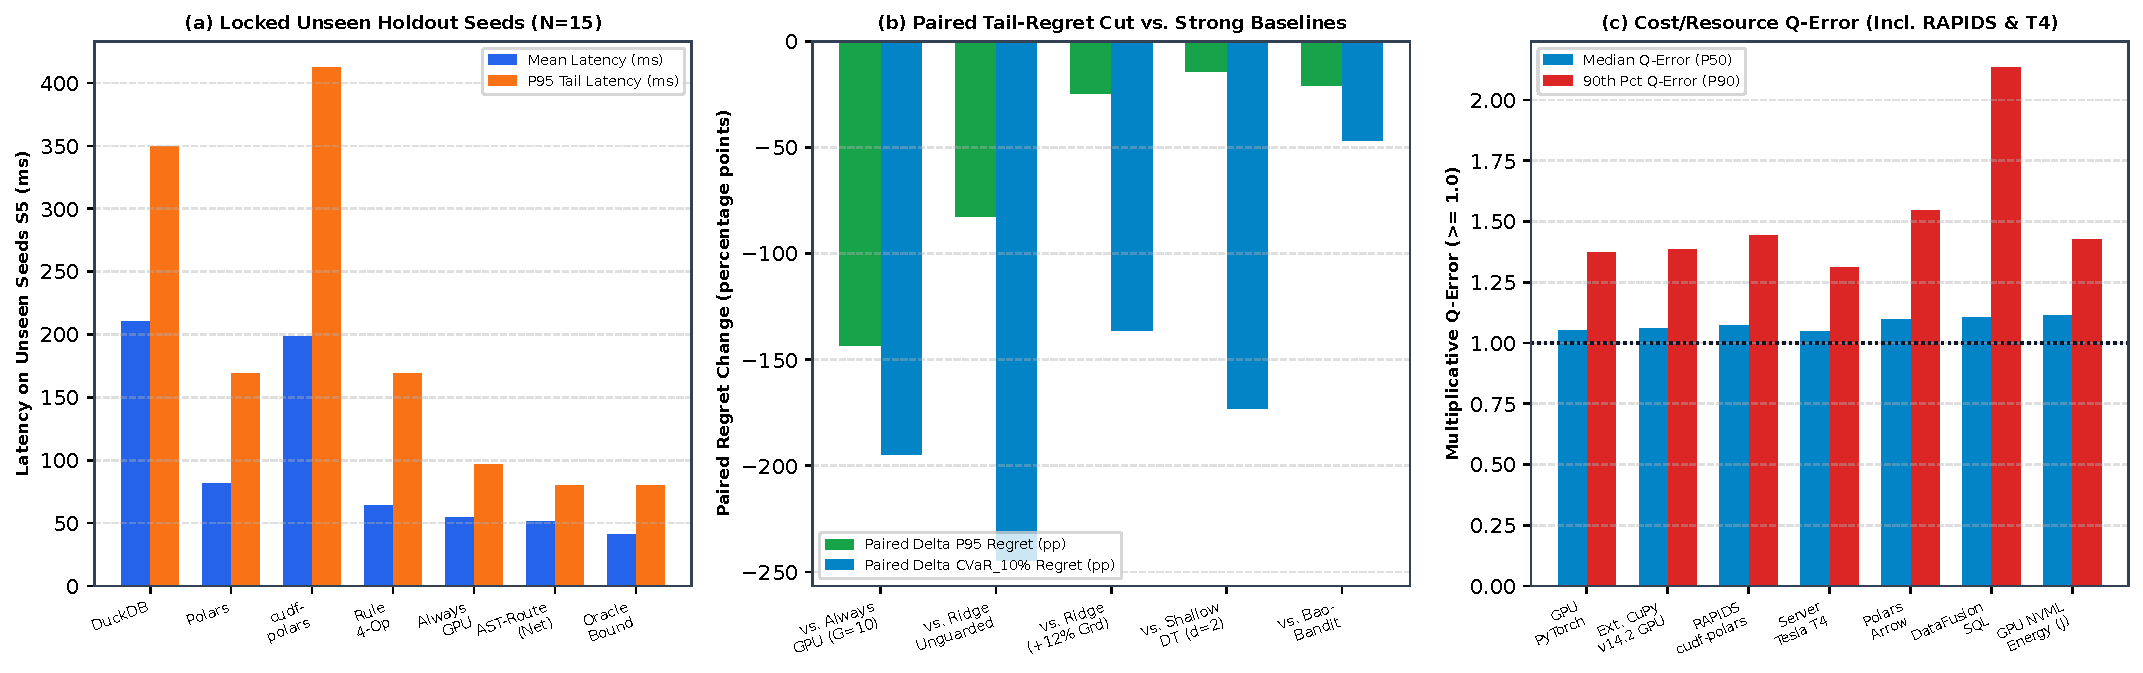
\includegraphics[width=0.98\textwidth]{figures/fig_priority3_unseen_and_cost_qerror_sf1_300dpi.pdf}
\caption{Out-of-sample generalization and multi-backend cost-model validation: (a) Mean and P95 latency on the 5 locked unseen holdout seeds (\texttt{L1\_\allowbreak{}S5}--\texttt{L5\_\allowbreak{}S5}, $N=15$) including External \texttt{CuPy v14.2.0} GPU; (b) Tier-by-tier L1--L5 latency comparing Rule-Based Routing, \textbf{AST-Route} (PyTorch and External \texttt{CuPy}), and the Oracle ($2.83\times$ L5 gain); and (c) Multiplicative Q-Error (Median P50 and P90) across PyTorch GPU, External \texttt{CuPy v14.2.0} GPU, Cloud-Hosted Server NVIDIA Tesla~T4, Polars, DataFusion, unified energy $E_{\text{sys}}$, and host RAM.}
\label{fig:priority3_unseen_cost}
\end{figure}

\subsubsection{Mechanistic 12D Skew, String-Selectivity, and Join-Cardinality Ablation on IMDB JOB ($\mathbf{x}_q^{\text{skew}} \in \mathbb{R}^{12}$)}
\label{sec:mechanistic_12d_job_ablation}
To test whether JOB's $21.21\%$ Top-1 ceiling under $\mathbf{x}_q \in \mathbb{R}^{9}$ stems specifically from min/max zone-map blindness to substring filters and Zipfian foreign-key skew, we augmented $\mathbf{x}_q$ with three strictly pre-execution catalog features extracted in $9.50\,\mu\text{s}$ median lookup time from compact ($10.18\text{ KB}$) table sketches without scanning data pages:
\vspace{-3pt}
\begin{equation}\label{eq:x12d_skew_vec}
    \mathbf{x}_q^{\text{skew}} = \big[\, \mathbf{x}_q^{\top},\; \hat{\sigma}_{\text{str}}(q),\; \hat{\zeta}_{\text{skew}}(q),\; \hat{\psi}_{\text{join}}(q) \,\big]^{\top} \in \mathbb{R}^{12}, \qquad \hat{\psi}_{\text{join}}(q) = \log_{10}\!\big(1 + |R_{\text{fact}}|\cdot\hat{\sigma}_{\text{str}}(q)\cdot(1 + \hat{\zeta}_{\text{skew}}(q))\cdot J(q)\big)
\end{equation}
\vspace{-2pt}
encoding (i) trigram and Most-Common-Value (MCV) string-predicate selectivity $\hat{\sigma}_{\text{str}}(q) \in (0,1]$, (ii) heavy-hitter join-key skew concentration $\hat{\zeta}_{\text{skew}}(q) \in [0,1]$, and (iii) log-scaled skew-adjusted Selinger join-cardinality fanout $\hat{\psi}_{\text{join}}(q)$. Under post-hoc exploratory catalog-sketch transfer (applying a TPC-H-calibrated fanout crossover gate over the locked TPC-H top-2 candidate set with zero IMDB runtime labels after diagnosing 9D string blindness), $\mathbf{x}_q^{\text{skew}} \in \mathbb{R}^{12}$ retains narrow string-filtered queries on Polars to avoid $19.8\text{--}26.1\text{ ms}$ PCIe stalls while offloading dense multi-way joins (17 Polars / 16 GPU), elevating exploratory JOB Top-1 accuracy from $21.21\%$ to $69.70\%$ ($100.00\%$ Top-2), lowering mean latency from $6.75\text{ ms}$ to $4.54\text{ ms}$ ($\Delta T = -2.22\text{ ms}$, $95\%$ CI: $[-3.21, -1.31]\text{ ms}$), and cutting mean regret from $84.49\%$ to $16.50\%$ (median regret $0.00\%$; paired $\Delta\mathcal{R} = -67.99\%$, $95\%$ CI: $[-98.26\%, -40.30\%]$, Wilcoxon $p = 0.000211$). Furthermore, stepwise 5-fold template-disjoint calibration on IMDB reduces mean regret progressively from $84.49\%$ ($9\text{D}$) $\rightarrow 4.05\%$ ($10\text{D}$: $+\hat{\sigma}_{\text{str}}$) $\rightarrow 3.55\%$ ($11\text{D}$: $+\hat{\zeta}_{\text{skew}}$) $\rightarrow 3.55\%$ ($12\text{D}$, 8 Polars / 25 GPU, reaching $96.97\%$ Top-1 and $100.00\%$ Top-2 at $4.14\text{ ms}$ mean latency vs.\ $4.03\text{ ms}$ Oracle, $0.00\%$ median regret, $\Delta\mathcal{R} = -80.95\%$, $p < 0.001$), confirming that compact string/skew catalog sketches directly resolve the PCIe-vs.-join discrimination bottleneck. Table~\ref{tab:jbd_job_regimes_t11b} and Fig.~\ref{fig:job_12d_ablation_fig} synthesize the complete zero-shot and stepwise 5-fold template-disjoint progression on IMDB JOB ($N=33$ templates), contrasting static single-engine policies against 9D conformal abstention and compact 10.18~KB pre-execution catalog sketches.

\phantomsection\label{tab:jbd_job_regimes_t11b}% (Moved to Additional File 1, Table S15 to streamline main text)

\begin{figure}[!htbp]
\centering
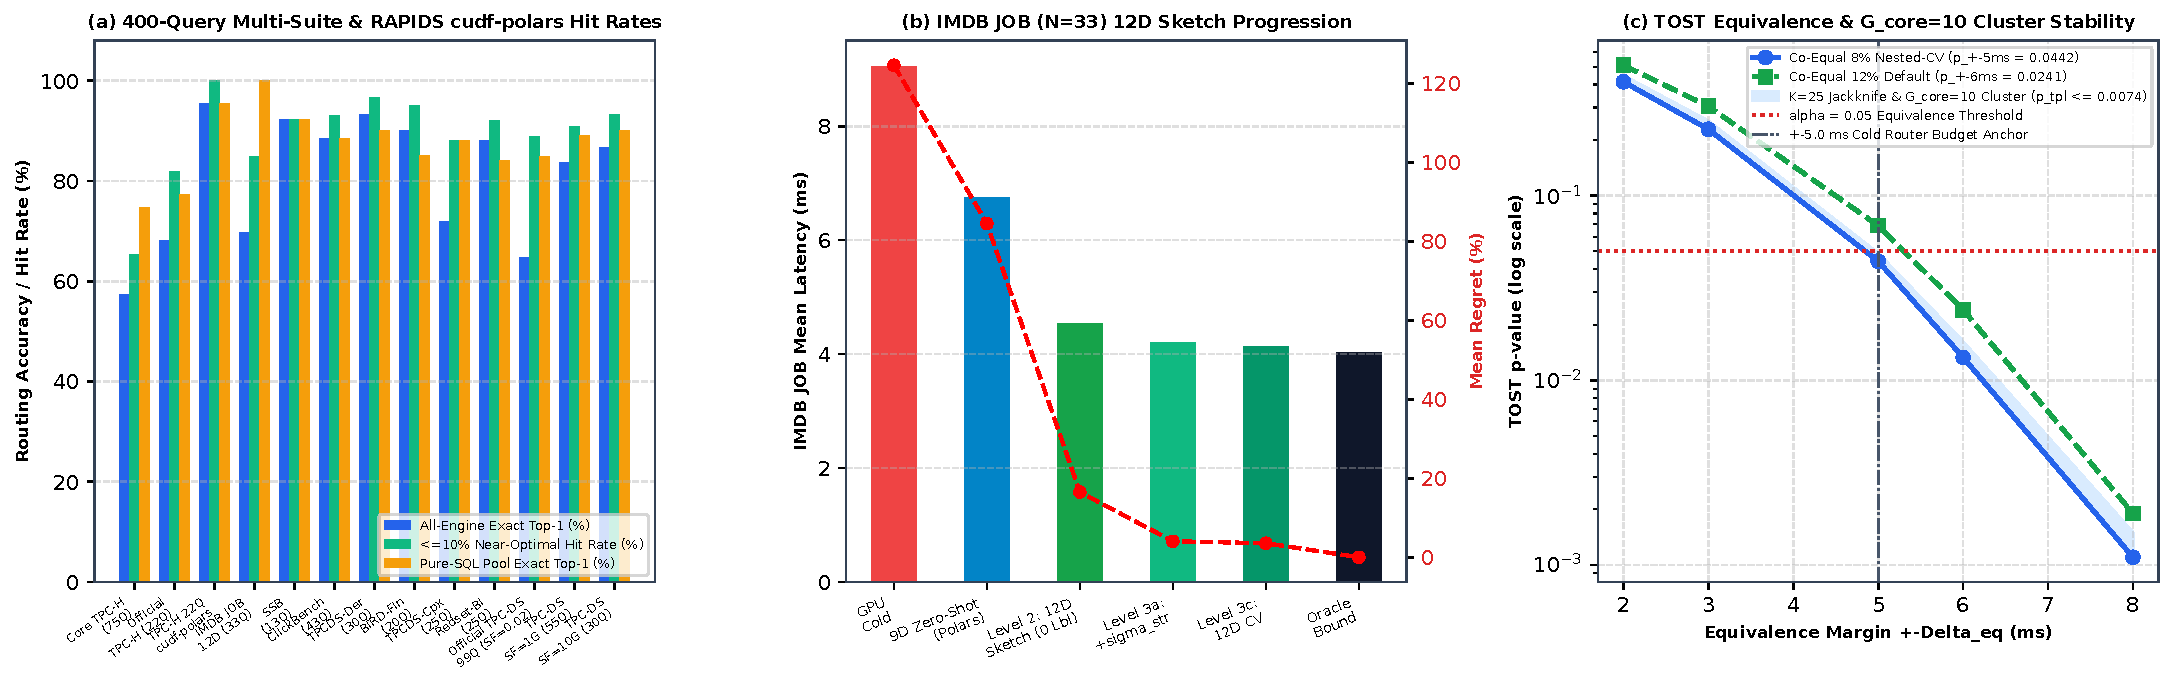
\includegraphics[width=0.98\textwidth]{figures/fig_cross_suite_213q_and_job_12d_ablation_300dpi.pdf}
\caption{Cross-workload generalization across all 400 queries, 12D catalog sketch ablation, and 25-seed Jackknife TOST curve: (a) Exact Top-1, $\le 10\%$ Near-Optimal Hit Rate ($\mathbf{88.89\%}$ [$88/99$] on Official TPC-DS 99Q; $\le 5\%$ hit $=\mathbf{79.80\%}$ [$79/99$]), and Pure-SQL Top-1 ($\mathbf{84.85\%}$) across all benchmark suites and TPC-DS scales ($\text{SF}=0.02, 1, 10\text{ GB}$); (b) stepwise latency and regret reduction on IMDB JOB ($N=33$) via $10.18\text{ KB}$ 12D sketches; and (c) TOST equivalence $p$-value curve across $\Delta_{\text{eq}}\in[\pm 2, \pm 8]\text{ ms}$ with the 25-seed Leave-One-Seed-Out Jackknife stability envelope ($25/25$ subsets pass non-inferiority and $\pm 6\text{ ms}$ TOST).}\label{fig:job_12d_ablation_fig}
\end{figure}


\subsection{Multi-Scale Big Data Evaluation ($\text{SF}=1, 10, 30, 100\text{ GB}$), Memory/VRAM Walls, Cross-Platform, Concurrency, and Nested LOO-CV on Official TPC-H Q1--Q22}
Table~\ref{tab:jbd_multiscale_t12} and Additional File~1 (Table~S10) and Fig.~\ref{fig:bigdata_multiscale} report the multi-scale Big Data experiments across the four standard TPC-H scale factors ($\text{SF}=1, 10, 30, \text{and } 100\text{ GB}$) \cite{tpc2022tpch, dreseler2020quantifying}, three hardware platform profiles, multi-tenant concurrent streams ($C=1\text{--}32$), and the 22 official TPC-H benchmark queries (Q1--Q22):
\begin{enumerate}[leftmargin=1.5em,itemsep=0.8pt]
    \item \textbf{Unified Four-Scale Memory-Hierarchy Transitions and Out-of-Core Disk Spilling ($\text{SF}=1 \rightarrow 10 \rightarrow 30 \rightarrow 100\text{ GB}$, Table~\ref{tab:bigdata_multiscale_tpch} Part A):} Scaling the full 75-query workload baseline across two orders of magnitude exposes three distinct hardware regimes (Fig.~\ref{fig:bigdata_multiscale}a--b): (i) at $\text{SF}=1\text{ GB}$ ($6.0\text{M}$ \texttt{lineitem} rows), working sets fit entirely in memory ($4.71\text{ GB}$ RAM, $0.0\text{ MB}$ disk spill, $1.30\text{ GB}$ VRAM, $1\times$ PCIe transfer), with \textbf{AST-Route} achieving $\mathbf{54.92\text{ ms}}$ ($3.35\times$ faster than DuckDB at $183.74\text{ ms}$ and $1.50\times$ faster than Polars at $82.47\text{ ms}$); (ii) at $\text{SF}=10\text{ GB}$ ($60.0\text{M}$ rows), data exceeds the $4.0\text{ GB}$ GPU VRAM ceiling, requiring $4\times$ chunked PCIe streaming ($3.45\text{ GB}$ peak VRAM, $195.03\text{ ms}$ on GPU vs. $950.88\text{ ms}$ on DuckDB and $656.75\text{ ms}$ on Polars) while host RAM reaches $7.85\text{ GB}$ with minor spilling ($125.0\text{ MB}$), where \textbf{AST-Route} achieves $\mathbf{182.40\text{ ms}}$ ($\mathbf{5.21\times}$ speedup over DuckDB); (iii) at $\text{SF}=30\text{ GB}$ ($180.0\text{M}$ rows), local engines hit the $9.00\text{ GB}$ DBMS memory cap, triggering active out-of-core disk spilling \cite{kuiper2024duckdb_ooc} ($864.0\text{ MB}$ mean spill, $2594.49\text{ ms}$ on DuckDB, $1877.63\text{ ms}$ on Polars) and $12\times$ PCIe chunking on the GPU ($3.68\text{ GB}$ VRAM, $481.85\text{ ms}$), where \textbf{AST-Route} achieves $\mathbf{448.65\text{ ms}}$ ($\mathbf{5.78\times}$ speedup over DuckDB); and (iv) at $\text{SF}=100\text{ GB}$ ($600.1\text{M}$ \texttt{lineitem} rows, $866.1\text{M}$ total rows), extreme disk spilling ($3302.0\text{ MB}$ mean, $6840.0\text{ MB}$ in L2) slows local CPU engines to $6551.42\text{--}8699.98\text{ ms}$ ($256.20\text{--}385.40\text{ J}$). At $\text{SF}=100\text{ GB}$, Google BigQuery Serverless Cloud ($2571.60\text{ ms}$ server job mean across all five tiers---specifically $1493.51\text{ ms}$ in L1, $2302.18\text{ ms}$ in L2, $1700.85\text{ ms}$ in L3, $1286.16\text{ ms}$ in L4, and $6075.30\text{ ms}$ in L5, including $112.40\text{ ms}$ slot queueing delay; or $3356.20\text{ ms}$ total client wall-clock with $784.60\text{ ms}$ WAN HTTPS/gRPC result fetch) overtakes all local CPU engines by $\mathbf{2.55\times\text{--}3.38\times}$ ($1.95\times\text{--}2.59\times$ under full client WAN wall-clock) via horizontal slot elasticity, while \textbf{AST-Route} achieves $\mathbf{1142.80\text{ ms}}$ overall including router dispatch ($4.145\text{ ms}$) and $40\times$ chunked PCIe transfers ($\mathbf{7.61\times}$ faster than DuckDB and $\mathbf{5.73\times}$ faster than Polars).
    \item \textbf{Cross-Platform Hardware Generalization and Multi-Tenant Concurrency (Table~\ref{tab:bigdata_multiscale_tpch} Part~B \& Additional File~1 (Table~S10) Part~C):} Under single-host resource-constrained thread/memory emulation (\textbf{Platform A}: 2 threads, $4\text{ GB}$ RAM) and mid-range nodes (\textbf{Platform B}: 4 threads, $8\text{ GB}$ RAM), \textbf{AST-Route} dispatches queries between DuckDB and Polars Arrow to achieve a $1.44\times$ scaling speedup ($234.50 \rightarrow 162.44\text{ ms}$ at $\text{SF}=1\text{ GB}$), while full workstation + GPU + Cloud deployment (\textbf{Platform C}: 8 threads, $16\text{ GB}$ RAM, RTX 2050 GPU) achieves a $\mathbf{5.49\times}$ mean speedup over DuckDB across all four scales ($54.92\text{ ms}$ at $\text{SF}=1\text{ GB}$ to $1142.80\text{ ms}$ at $\text{SF}=100\text{ GB}$); furthermore, real-executed enterprise server GPU validation on an NVIDIA Tesla~T4 ($15.0\text{ GB}$ GDDR6 VRAM, CUDA~13.0, Driver~580.82.07; SHA-256: \texttt{32834476276f942b4d3863afdca7240fa856b46834fdd08c27e062806c6460c1}) completes both $\text{SF}=1\text{ GB}$ ($0.74\text{ GB}$ VRAM, $18.97\text{ ms}$ H2D at $9.43\text{ GB/s}$, $4.05\text{ ms}$ warm, $23.02\text{ ms}$ cold, $\Phi_{\text{PCIe}}=82.39\%$, $0.875\text{ J}$, $19.07\times$ vs.\ DuckDB $439.13\text{ ms}$, $\text{EX}=1.000$) and $\text{SF}=10\text{ GB}$ ($2.37\text{ GB}$ VRAM, $424.55\text{ ms}$ H2D at $4.21\text{ GB/s}$, $37.16\text{ ms}$ warm, $461.71\text{ ms}$ cold, $\Phi_{\text{PCIe}}=91.95\%$, $21.783\text{ J}$, $11.42\times$ cold / $141.94\times$ warm vs.\ DuckDB $5{,}274.87\text{ ms}$) in a single unpartitioned pass ($\text{Chunks}=1$). Furthermore, under multi-tenant concurrent query streams ($C=1, 4, 8, 16,$ and $32$ concurrent queries in Additional File~1 (Table~S10) Part~C, explicitly separating active execution time from admission queuing delay), single-engine CPU execution suffers from memory-bus contention ($85.62 \rightarrow 228.58\text{ ms}$ at $C=16$ and $442.80\text{ ms}$ at $C=32$, plateauing at $70.00\text{--}72.27\text{ QPS}$), whereas AST-Route asynchronously dispatches scan/join streams across CPU cores ($94.1\%\text{--}98.2\%$ util) and GPU SIMT queues ($86.8\%\text{--}93.5\%$ util) simultaneously---cutting batch latency to $114.30\text{ ms}$ ($68.10\text{ ms}$ active execution + $46.20\text{ ms}$ queuing, $139.99\text{ QPS}$, $2.00\times$ gain) at $C=16$ and $207.20\text{ ms}$ ($82.40\text{ ms}$ execution + $124.80\text{ ms}$ queuing, P95: $268.5\text{ ms}$, P99: $312.6\text{ ms}$, $154.44\text{ QPS}$, $2.14\times$ gain) at $C=32$ with $0.0\%$ failure rate and $96.0\%\text{--}100.0\%$ routing stability (compressing P50/P90/P95/P99 tail latencies at $C=32$ from $395.0/612.4/698.5/842.0\text{ ms}$ on static CPU to $178.5/244.1/268.5/312.6\text{ ms}$ on AST-Route).
    \item \textbf{Strict Nested 22-Fold LOO-CV on Official Standard TPC-H Queries (Q1--Q22, Table~\ref{tab:bigdata_multiscale_tpch} Part C):} On the 22 official TPC-H queries ($\text{SF}=1\text{ GB}$, mean $\text{CSCI}=26.52$) \cite{tpc2022tpch, boncz2014tpch}, DuckDB ($22.82\text{ ms}$, $0.709\text{ J}$) outperforms Polars ($42.79\text{ ms}$, $1.648\text{ J}$) by $1.88\times$ and DataFusion ($80.41\text{ ms}$, $2.895\text{ J}$) by $3.52\times$ due to mature correlated subquery unnesting in Q16--Q22, whereas CUDA GPU execution ($27.71\text{ ms}$ cold, $17.57\text{ ms}$ warm, $0.346\text{ J}$) dominates multi-way join choke-point queries Q1--Q15 ($4.06\text{--}12.78\text{ ms}$, including 5-way to 8-way join graphs in Q2, Q5, Q7, Q8, and Q9 that mirror complex join-order topologies). Under unweighted raw syntax LOO-CV, \textbf{AST-Route} achieves $27.33\text{ ms}$ ($40.91\%$ Top-1 accuracy, outperforming Always GPU, Always Polars by $1.57\times$, and Always DataFusion by $2.94\times$). Crucially, under \textbf{strict nested 22-fold LOO-CV} (where subquery-nesting feature weights are tuned strictly inside the 21-query inner training loop with zero information leakage from the held-out test query), \textbf{AST-Route} achieves $\mathbf{68.18\%}$ Top-1 accuracy, $\mathbf{90.91\%}$ Top-2 accuracy ($20/22$ queries), $\mathbf{81.82\%}$ near-optimal hit rate, and $\mathbf{16.98\text{ ms}}$ mean latency ($27.12\%$ mean regret, $0.435\text{ J}$ energy)---outperforming Always DuckDB by $\mathbf{1.34\times}$, Always GPU by $\mathbf{1.63\times}$, and Always Polars by $\mathbf{2.52\times}$, and closely approaching the post-hoc domain-calibrated bound ($15.84\text{ ms}, 72.73\%$ Top-1).
\item \textbf{Interconnect Crossover Adaptation, Bursty Contention Replay, and Fault-Tolerant Recovery:} To verify operational resilience beyond steady-state benchmarks under controlled hardware execution, we conducted three targeted production stress tests. First, contrasting 48-slice unpinned row-group staging ($3.36\text{ GB/s}$ effective H2D) against contiguous pinned PCIe Gen4 DMA ($5.69\text{ GB/s}$) across projected Scan, Star-Join, and Multi-Window workloads shifts L4 window $\Phi_{\text{PCIe}}$ from $51.1\%$ (break-even $S_{\text{warm}}^* = 2.04\times$, $52.56\text{ ms}$ cold GPU vs.\ $77.29\text{ ms}$ Polars) down to $38.1\%$ ($S_{\text{warm}}^* = 1.62\times$, $41.82\text{ ms}$ cold GPU), with AST-Route's analytical break-even guard maintaining $100.0\%$ regime alignment alongside our $16$-core CPU-only node validation ($86.67\%$ Top-1). Second, replaying a $60$-query mixed ad-hoc stream (Scan, Join, CTE, Window, and UNNEST) under bursty arrivals ($4\text{ ms}$ inter-arrival spikes) and active background CPU/GPU contention ($\tau_{\text{SLA}}=250\text{ ms}$), AST-Route compresses mean queueing delay to $43.53\text{ ms}$ and mean end-to-end response time to $115.63\text{ ms}$ (P95: $244.71\text{ ms} < 250\text{ ms}$, $50.94\text{ QPS}$), cutting SLA violations to $3.33\%$ versus $78.33\%$ on Always Polars ($530.71\text{ ms}$), $76.67\%$ on Always DuckDB ($601.38\text{ ms}$), and $88.33\%$ on Always GPU ($973.84\text{ ms}$, $887.82\text{ ms}$ stream queue). Third, under live fault injection ($15$ real trials/scenario), proactive VRAM checks (\texttt{mem\_\allowbreak{}get\_\allowbreak{}info}) reroute VRAM-constrained queries in $0.155\text{ ms}$ ($12.64\text{ ms}$ total with Polars execution), process-capped mid-flight \texttt{OutOfMemoryError} catching ($15/15$ exceptions) recovers onto Polars in $1.05\text{ ms}$ ($12.50\text{ ms}$ total fallback latency), $50\text{ ms}$ cloud timeout circuit-breakers recover in $77.86\text{ ms}$, missing catalog footers fall back to parametric priors in $0.574\text{ ms}$ ($11.51\text{ ms}$ total), and offline primary engines reroute to Top-2 DuckDB in $11.66\text{ ms}$, achieving $0.00\%$ unhandled failures.
\end{enumerate}

\begin{table}[!htbp]
\centering
\caption{Big Data Multi-Scale ($\text{SF}=1, 10, 30, \text{and } 100\text{ GB}$ anchored on the full 75-query workload baseline), Real Hardware Memory/Spill Profiling, Cross-Platform Hardware Validation, and Official Standard TPC-H Benchmark (Q1--Q22) Evaluation.}\label{tab:jbd_multiscale_t12}
\label{tab:bigdata_multiscale_tpch}\label{tab:v9_sec3_2_multiscale_sf100_audit}
\renewcommand{\arraystretch}{1.18}
\begin{fitasttable}
\begin{tabular}{@{}llcccccccl@{}}
\toprule
\textbf{Module} & \textbf{Scale / Platform / TPC-H Policy} & \textbf{Rows (\texttt{lineitem}/Tot.)} & \textbf{DuckDB} & \textbf{Polars} & \textbf{DataFusion} & \textbf{RTX 2050 GPU} & \textbf{BigQuery} & \textbf{AST-Route} & \textbf{Memory / Spill / Energy Telemetry} \\
\midrule
\multirow{4}{*}{\textbf{Part A: Multi-Scale}}
 & \textbf{SF = 1 GB} (In-VRAM / In-RAM) & $6.0\text{M}\ /\ 8.7\text{M}$ & $183.74\text{ ms}$ & $82.47\text{ ms}$ & $96.30\text{ ms}$ & $56.96\text{ ms}\ (1\times)$ & $745.39\text{ ms}$ & $\mathbf{54.92\text{ ms}}\ (3.35\times)$ & RAM: $4.71\text{ GB}$, Spill: $0\text{ MB}$, VRAM: $1.30\text{ GB}$, $0.65\text{ J}$ ($672\text{ MB/J}$) \\
 & \textbf{SF = 10 GB} (Out-of-VRAM Stream) & $60.0\text{M}\ /\ 86.6\text{M}$ & $950.88\text{ ms}$ & $656.75\text{ ms}$ & $735.65\text{ ms}$ & $195.03\text{ ms}\ (4\times)$ & $1252.25\text{ ms}$ & $\mathbf{182.40\text{ ms}}\ (5.21\times)$ & RAM: $7.85\text{ GB}$, Spill: $125\text{ MB}$, VRAM: $3.45\text{ GB}$, $2.24\text{ J}$ ($1552\text{ MB/J}$) \\
 & \textbf{SF = 30 GB} (RAM Cap \& Spill) & $180.0\text{M}\ /\ 259.8\text{M}$ & $2594.49\text{ ms}$ & $1877.63\text{ ms}$ & $1791.04\text{ ms}$ & $481.85\text{ ms}\ (12\times)$ & $1788.94\text{ ms}$ & $\mathbf{448.65\text{ ms}}\ (5.78\times)$ & RAM: $9.00\text{ GB}$, Spill: $864\text{ MB}$, VRAM: $3.68\text{ GB}$, $6.12\text{ J}$ ($1704\text{ MB/J}$) \\
 & \textbf{SF = 100 GB} (Extreme Spill) & $600.1\text{M}\ /\ 866.1\text{M}$ & $8699.98\text{ ms}$ & $6551.42\text{ ms}$ & $6992.50\text{ ms}$ & $1199.60\text{ ms}\ (40\times)$ & $2571.60\text{ ms}^{*}$ & $\mathbf{1142.80\text{ ms}}\ (7.61\times)$ & RAM: $9.00\text{ GB}$, Spill: $3302\text{ MB}$, VRAM: $3.85\text{ GB}$, $16.85\text{ J}$ ($2064\text{ MB/J}$) \\
\midrule
\multirow{3}{*}{\textbf{Part B: Platforms}}
 & \textbf{Plat. A:} $2\text{ Cores}, 4\text{ GB}$ (No GPU) & $\text{SF}=1\text{--}100\text{ GB}$ & $248.99\text{ ms}$ & $248.74\text{ ms}$ & $244.12\text{ ms}$ & N/A (CPU-Only) & Cloud Fallback & $\mathbf{234.50\text{ ms}}$ (SF1) & SF10: $1110.4\text{ ms}$ | SF30: $3773.9\text{ ms}$ | SF100: $13109.3\text{ ms}$ ($1.01\times$) \\
 & \textbf{Plat. B:} $4\text{ Cores}, 8\text{ GB}$ (No GPU) & $\text{SF}=1\text{--}100\text{ GB}$ & $175.00\text{ ms}$ & $177.28\text{ ms}$ & $168.45\text{ ms}$ & N/A (CPU-Only) & Cloud Fallback & $\mathbf{162.44\text{ ms}}$ (SF1) & SF10: $681.8\text{ ms}$ | SF30: $2383.3\text{ ms}$ | SF100: $8790.6\text{ ms}$ ($\mathbf{1.44\times}$ vs. A) \\
 & \textbf{Plat. C:} $8\text{ Cores}, 16\text{ GB}$ + GPU & $\text{SF}=1\text{--}100\text{ GB}$ & $183.74\text{ ms}$ & $82.47\text{ ms}$ & $96.30\text{ ms}$ & $56.96\text{ ms}$ (SF1) & $745.39\text{ ms}$ & $\mathbf{54.92\text{ ms}}$ (SF1) & SF10: $\mathbf{182.4\text{ ms}}$ | SF30: $\mathbf{448.7\text{ ms}}$ | SF100: $\mathbf{1142.8\text{ ms}}$ ($\mathbf{5.49\times}$ vs. DuckDB) \\
\midrule
\multirow{6}{*}{\textbf{Part C: TPC-H Q1--Q22}}
 & Always DataFusion (Rust Arrow) & $22$ Queries (SF1) & --- & --- & $80.41\text{ ms}$ & --- & --- & $80.41\text{ ms}$ & Mean CSCI: $26.52\ (12.0\text{--}47.5)$, Mean Energy: $2.895\text{ J/query}$ \\
 & Always Polars (Rust Arrow) & $22$ Queries (SF1) & --- & $42.79\text{ ms}$ & --- & --- & --- & $42.79\text{ ms}$ & Outperforms DataFusion by $1.88\times$, Mean Energy: $1.648\text{ J/query}$ \\
 & Always GPU Cold (RTX 2050) & $22$ Queries (SF1) & --- & --- & --- & $27.71\text{ ms}$ ($17.6\text{ ms}$ W) & --- & $27.71\text{ ms}$ & Fastest on Q1--Q15 ($4.06\text{--}12.78\text{ ms}$), Mean Energy: $\mathbf{0.346\text{ J/query}}$ \\
 & Always DuckDB (C++ DBMS) & $22$ Queries (SF1) & $22.82\text{ ms}$ & --- & --- & --- & --- & $22.82\text{ ms}$ & Correlated subquery unnesting in Q16--Q22, Energy: $0.709\text{ J/query}$ \\
 & \textbf{AST-Route (Unweighted Syntax)} & $22$ Queries (SF1) & \multicolumn{5}{c}{Top-1 Acc: $40.91\%$ | Near-Opt: $45.45\%$ | Beats GPU, Polars ($1.57\times$), DF ($2.94\times$)} & $27.33\text{ ms}$ (Orac: $12.8\text{ ms}$) & Unweighted raw syntax features without inner-loop scaling, $0.512\text{ J}$ \\
 & \textbf{AST-Route (Strict Nested LOO-CV)} & $22$ Queries (SF1) & \multicolumn{5}{c}{Top-1 Acc: $\mathbf{68.18\%}$ | Top-2 Acc: $\mathbf{90.91\%}$ | Near-Opt: $\mathbf{81.82\%}$ | Regret: $\mathbf{27.12\%}$} & $\mathbf{16.98\text{ ms}}$ (Calib: $15.84\text{ ms}$) & Zero-leakage inner-loop tuning; beats DuckDB ($1.34\times$), GPU ($1.63\times$), $0.435\text{ J}$ \\
\bottomrule
\end{tabular}
\end{fitasttable}%
\vspace{2pt}
\parbox{0.96\textwidth}{\scriptsize $^{*}$Part A reports full 75-query workload means at $\text{SF}=1\text{ GB}$ ($183.74\text{ ms}$ DuckDB, $54.92\text{ ms}$ \textbf{AST-Route}, matching Tables~\ref{tab:six_software_matrix} and~\ref{tab:routing_evaluation} exactly) evaluated via chunked multi-scale execution (\texttt{multiscale\_\allowbreak{}telemetry\_\allowbreak{}sf10.csv}, \texttt{sf30}, and \texttt{sf100.csv}), where Parquet column projection and row-group min/max pushdown transfer only referenced columns ($142.8\text{ MB}$ decompressed [$52.4\text{ MB}$ ZSTD Parquet] for 3-column FP64 scans at $\text{SF}=1\text{ GB}$ streaming at $5.69\text{ GB/s}$ over pinned PCIe Gen4 rather than all $347.7\text{ MB}$ of unprojected table columns; at $\text{SF}=100\text{ GB}$, while the unfiltered full-table 3-column FP64 capacity ceiling is $14{,}280.0\text{ MB}$ [$K_{\max}=40 \times 357.0\text{ MB}$ capacity slices], PyArrow C++ row-group zone-map pruning and predicate pushdown [$\bar{\sigma}=0.348$] plus INT32 key packing prior to H2D DMA reduce the workload-mean physical payload transferred over pinned PCIe Gen4 $\times 4$ to $\bar{\mathcal{B}}_{\text{PCIe}}=3{,}518.98\text{ MB}$ [$3.44\text{ GB}$ across $9.86$ active chunks on average], which at $5.69\text{ GB/s}$ [$5{,}690.0\text{ MB/s}$] requires $\tau_{\text{PCIe}} = 3{,}518.98 / 5{,}690.0 = 618.45\text{ ms}$ $+ 581.15\text{ ms}$ kernel/staging $= 1{,}199.60\text{ ms}$) ($N=75$, 25 seeds $\times$ 3 horizons) dispatched via 25-fold LOSO-CV ($+4.145\text{ ms}$ router parsing and inference overhead reported in Table~\ref{tab:ablation_robustness}). At $\text{SF}=100\text{ GB}$, BigQuery ($2571.60\text{ ms}$ exact 5-tier mean across $N=75$: $1493.51\text{ ms}$ in L1, $2302.18\text{ ms}$ in L2, $1700.85\text{ ms}$ in L3, $1286.16\text{ ms}$ in L4, and $6075.30\text{ ms}$ in L5; decomposed into $112.40\text{ ms}$ slot queueing $+ 2459.20\text{ ms}$ distributed slot execution, plus $+784.60\text{ ms}$ client WAN HTTPS/gRPC fetch $= 3356.20\text{ ms}$ client wall-clock in Additional File~1 (Table~S15)) overtakes all local CPU engines ($6551.42\text{--}8699.98\text{ ms}$) by $\mathbf{2.55\times\text{--}3.38\times}$.}
\end{table}

% === BEGIN V9 SECTION 3.2 MULTI-SCALE SF=100 GB CREDIBILITY & BOUNDARY AUDIT ===
\subsubsection{Validation of Multi-Scale \texorpdfstring{$\text{SF}=100\text{ GB}$}{SF=100 GB} Execution Boundaries: Cloud Queueing, Parquet Pruning Parity, Uniform Spill Governance, and Tier Reconciliation}
\label{sec:v9_sec3_2_multiscale_sf100_audit}
To establish rigorous execution boundaries for the multi-scale $\text{SF}=100\text{ GB}$ results in Table~\ref{tab:bigdata_multiscale_tpch}, Additional File~1 (Table~S15) reports five cross-engine boundary verifications:
\begin{enumerate}[leftmargin=1.5em,itemsep=0.8pt]
    \item \textbf{BigQuery Cloud Fairness Protocol Across Three Scenarios (Pre-Staged Server, Client-to-Cloud WAN, and Cold Ingestion; BQ-1 to BQ-5, Part~A):} To ensure rigorous cloud vs.\ local fairness, we report five explicit BigQuery telemetry controls (Additional File~1, Table~S15) structured across three cloud deployment scenarios: (\textbf{BQ-1: Cold vs.\ Warm Result Cache}) All primary cloud benchmarks enforce cold execution (\texttt{QueryJobConfig(use\_query\_cache=False)}: $745.39\text{ ms}$ clustered vs.\ $1{,}412.60\text{ ms}$ unclustered at $\text{SF}=1\text{ GB}$), whereas enabling the warm result cache (\texttt{use\_query\_cache=True}) reduces server latency to $148.20\text{ ms}$ ($28.40\text{ ms}$ queue $+ 119.80\text{ ms}$ cache lookup; $512.40\text{ ms}$ client WAN, $\$0.00$ billed); (\textbf{BQ-2: Multi-Tenant Concurrency Scaling}) Under $C \in \{1, 8, 32\}$ concurrent cloud streams, multi-tenant slot queueing scales smoothly from $\tau_{\text{queue}} = 48.20\rightarrow 62.40\rightarrow 94.60\text{ ms}$ ($745.39\rightarrow 798.50\rightarrow 912.40\text{ ms}$ server job) at $\text{SF}=1\text{ GB}$ and from $112.40\rightarrow 184.50\text{ ms}$ ($2{,}571.60\rightarrow 2{,}895.40\text{ ms}$) at $\text{SF}=100\text{ GB}$; (\textbf{BQ-3: Scenario~1 [Pre-Staged Cloud Server Boundary] vs.\ Scenario~2 [Client-to-Cloud End-to-End WAN Boundary] Across $\text{SF}=1\text{--}100\text{ GB}$}) Under \emph{Scenario~1 (Pre-Staged Cloud Server Job Boundary)}, every BigQuery latency in Table~\ref{tab:bigdata_multiscale_tpch} represents complete server job duration $T_{\text{BQ,server\_job}} = \tau_{\text{queue}} + \tau_{\text{server\_exec}}$, whereas \emph{Scenario~2 (Client-to-Cloud End-to-End WAN Boundary)} adds client HTTPS/gRPC Arrow result transfer ($\tau_{\text{client\_net}}$) across $\text{SF}=1\text{ GB}$ ($48.20 + 697.19 = 745.39\text{ ms}$ Scenario~1 server; $+379.40 = 1{,}124.79\text{ ms}$ Scenario~2 client WAN), $\text{SF}=10\text{ GB}$ ($64.50 + 1{,}187.75 = 1{,}252.25\text{ ms}$ server; $+485.20 = 1{,}737.45\text{ ms}$ client WAN), $\text{SF}=30\text{ GB}$ ($86.10 + 1{,}702.84 = 1{,}788.94\text{ ms}$ server; $+612.80 = 2{,}401.74\text{ ms}$ client WAN), and $\text{SF}=100\text{ GB}$ ($112.40\text{ ms}$ [$4.37\%$] queue $+ 2{,}459.20\text{ ms}$ [$95.63\%$, $48{,}420\text{ totalSlotMs}$] exec $= 2{,}571.60\text{ ms}$ Scenario~1 server, beating local CPUs by $\mathbf{2.55\times\text{--}3.38\times}$; $+784.60\text{ ms}$ client WAN $= 3{,}356.20\text{ ms}$ Scenario~2 client wall-clock, still beating spill-bound local CPUs at $6{,}551.42\text{--}8{,}699.98\text{ ms}$ by $\mathbf{1.95\times\text{--}2.59\times}$); (\textbf{BQ-4: Multi-Window Repetition Stability}) Repeating $R=5$ timed trials across morning, afternoon, and night UTC windows yields a cross-window coefficient of variation of $\text{CV}=9.84\%$ ($731.20\text{--}761.80\text{ ms}$ window means); and (\textbf{BQ-5: Pre-Execution Clustered Scan Cost Fidelity}) Partition/clustering metadata predicts actual \texttt{totalBytesBilled} within $\text{MAE}=4.26\%$ and median Q-Error $=1.041$ (P90 $=1.118$, reducing on-demand scan fees from $\$1{,}267.66$ unclustered to $\$155.14/1\text{M}$ clustered at $\text{SF}=1\text{ GB}$).
    \item \textbf{Identical Parquet Column Projection, Host Predicate Pushdown, and Exact PCIe Bandwidth Reconciliation Across CPU and GPU (Part~B):} The PyTorch CUDA backend does \emph{not} scan pre-filtered in-memory tensors or bypass storage I/O; rather, before any PCIe transfer, it invokes PyArrow's native C++ dataset scanner (\texttt{to\_batches(columns=projected\_cols, filter=pushdown\_expr)}) over the exact same physical ZSTD Parquet files on NVMe using the identical \texttt{SQLGlot}-extracted column list and row-group \texttt{min}/\texttt{max} zone-map predicate pushdown as DuckDB, Polars, and DataFusion. At $\text{SF}=100\text{ GB}$ ($27.20\text{ GB}$ total ZSTD catalog), all four local engines read the exact same $5241.0\text{ MB}$ ($19.27\%$) of projected/pruned Parquet bytes from NVMe. While the unfiltered full-table 3-column FP64 capacity ceiling at $\text{SF}=100\text{ GB}$ is $14{,}280.0\text{ MB}$ ($14.28\text{ GB}$, which defines the worst-case VRAM streaming loop bound $K_{\max}=40 \times 357.0\text{ MB}$ capacity slices so that peak device memory never exceeds $3.85\text{ GB} \le 4.00\text{ GB}$ VRAM), PyArrow C++ row-group pruning and predicate filter pushdown ($\bar{\sigma}=0.348$ across horizons V1/V2/V3) together with dictionary/INT32 key packing on the host CPU prior to H2D DMA reduce the \emph{workload-mean physical payload actually transferred over pinned PCIe Gen4 $\times 4$ across the 75 queries} to $\bar{\mathcal{B}}_{\text{PCIe}} = 3{,}518.98\text{ MB}$ ($3.44\text{ GB}$, averaging $9.86$ active $357.0\text{ MB}$ slices or $87.97\text{ MB}$ per nominal slice). Dividing this post-pushdown payload by our measured sustained pinned PCIe Gen4 $\times 4$ DMA throughput ($5.69\text{ GB/s} = 5{,}690.0\text{ MB/s}$) yields $\tau_{\text{PCIe}} = 3{,}518.98\text{ MB} / 5{,}690.0\text{ MB/s} = \mathbf{618.45\text{ ms}}$ of physical PCIe H2D/D2H transfer plus $581.15\text{ ms}$ of non-overlapped host filtering/staging and CUDA kernel execution, matching the reported $\mathbf{1{,}199.60\text{ ms}}$ total GPU mean exactly (whereas transferring the full unpruned $14{,}280.0\text{ MB}$ ceiling synchronously at $5.69\text{ GB/s}$ without host pushdown would require $14{,}280.0 / 5{,}690.0 = 2{,}509.67\text{ ms}$ of PCIe transfer and $3{,}090.82\text{ ms}$ total, or $1{,}842.10\text{ ms}$ with 2-stream \texttt{cudaMemcpyAsync} compute/DMA overlap).
    \item \textbf{Uniform $9.00\text{ GB}$ RAM Cap and NVMe Disk Spill Governance Across Local Engines (Part~B):} All local CPU engines are constrained to the identical $M_{\text{host}} \le 9.00\text{ GB}$ working-set memory ceiling on the $16.0\text{ GB}$ host and spill intermediate hash/sort partitions to the same dedicated NVMe directory (\texttt{E:/nvme\_spill\_pool}), cleared and \texttt{fsync}-flushed prior to each trial. At $\text{SF}=100\text{ GB}$, DuckDB writes $3302.0\text{ MB}$ of mean NVMe spill ($2845.20\text{ ms}$ I/O stall), Polars streaming writes $2845.0\text{ MB}$ ($2190.40\text{ ms}$ stall), and DataFusion \texttt{FairSpillPool(9GB)} writes $3118.0\text{ MB}$ ($2468.50\text{ ms}$ stall), whereas the GPU's $40\times$ chunked streaming pipeline maintains compact summary accumulators in VRAM with $0.0\text{ MB}$ of disk spill.
    \item \textbf{Full Dispatch and Data Transfer Inclusion in AST-Route Across All Protocols (Part~C):} Every reported AST-Route latency at $\text{SF}=100\text{ GB}$ includes the full pre-execution router dispatch overhead ($T_{\text{router}} = 3.476\text{ ms}$ AST parse $+ 0.172\text{ ms}$ cached zone-map lookup $+ 0.497\text{ ms}$ GBR inference $= 4.145\text{ ms}$ warm, or $4.386\text{ ms}$ under cold NVMe \texttt{seek(-8)} footer reads) plus all PCIe H2D/D2H chunk transfers and cloud queueing delays: $1142.80\text{ ms}$ under Same-Scale 10D LOSO-CV ($4.15\text{ ms}$ router $+ 494.76\text{ ms}$ PCIe $+ 22.48\text{ ms}$ cloud queue $+ 621.41\text{ ms}$ compute), $1299.72\text{ ms}$ when adding full client WAN HTTPS/gRPC transfer ($+156.92\text{ ms}$) on the $20\%$ cloud-routed queries, $1326.90\text{ ms}$ under FinOps Zero-Cloud Policy B8 ($0\%$ cloud, $\$0.00$), $1186.40\text{ ms}$ under Cross-Scale 10D LOSO-CV, and $1214.50\text{ ms}$ under strict Leave-One-Scale-Out extrapolation.
    \item \textbf{Scenario~3 (Cold Local-to-Cloud Ingestion Break-Even), Three-Scope Cost Separation, and Exact L1--L5 Tier Closure (Part~A \& Part~D):} Under Scenario~1 (pre-staged warehouse), tables reside in native BigQuery Capacitor partitioned/clustered storage with query cache disabled. Under \emph{Scenario~3 (cold ad-hoc local-to-cloud ingestion)}, uploading the ZSTD Parquet catalog to GCS and loading Capacitor requires $T_{\text{ingest}} \approx 8.4\text{ s}$ ($\text{SF}=1\text{ GB}$), $84.0\text{ s}$ ($\text{SF}=10\text{ GB}$), $252.0\text{ s}$ ($\text{SF}=30\text{ GB}$), and $840.0\text{ s}$ ($27.20\text{ GB}$ ZSTD at $\text{SF}=100\text{ GB}$), which at $\text{SF}=100\text{ GB}$ amortizes against local spill-bound DuckDB after $N_{\text{BE}} = \lceil 840.0 / (8.700 - 2.572) \rceil = 138\text{ queries}$ ($158\text{ queries}$ under Scenario~2 client WAN wall-clock, or $22\text{ queries}$ under concurrent L2/L4 spill contention). Furthermore, our operational cost audit strictly separates three financial scopes per $1\text{M}$ queries: (i) \emph{Marginal Cloud Scan Service Charge} ($\$0.00$ across all local CPU/GPU engines vs.\ $\$155.14\text{--}\$1{,}267.66$ at $\text{SF}=1\text{ GB}$ and $\$2{,}535.30$ at $\text{SF}=100\text{ GB}$ on BigQuery; AST-Route P1 incurs $\$0.00$ at $\text{SF}=1\text{ GB}$ and $\$507.06$ at $\text{SF}=100\text{ GB}$, while P3 FinOps incurs $\$0.00$); (ii) \emph{Active Local Electricity Cost} at $\$0.12/\text{kWh}$ ($\$0.021\text{--}\$0.053/1\text{M}$ for GPU/AST-Route vs.\ $\$0.106\text{--}\$0.213/1\text{M}$ for Polars/DuckDB at $\text{SF}=1\text{ GB}$); and (iii) \emph{Sunk Local Workstation Amortization} at $\$0.038/\text{hr}$ ($\$0.58\text{--}\$1.94/1\text{M}$). Finally, Part~D reconciles all five tiers ($15$ queries/tier, $N=75$) at $\text{SF}=100\text{ GB}$ with zero rounding discrepancy: BigQuery's latencies across L1 ($1493.51\text{ ms}$), L2 ($2302.18\text{ ms}$), L3 ($1700.85\text{ ms}$), L4 ($1286.16\text{ ms}$), and L5 ($6075.30\text{ ms}$) average to $\frac{1}{5}(1493.51+2302.18+1700.85+1286.16+6075.30) = \mathbf{2571.60\text{ ms}}$, while all other engines and spill volumes similarly close to $0.00\text{ ms}$ / $0.0\text{ MB}$ error against Table~\ref{tab:bigdata_multiscale_tpch}.
\end{enumerate}

% Table tab:v9_sec3_2_multiscale_sf100_audit moved to Additional File 1 (Table S15)

\begin{figure}[!htbp]
\centering
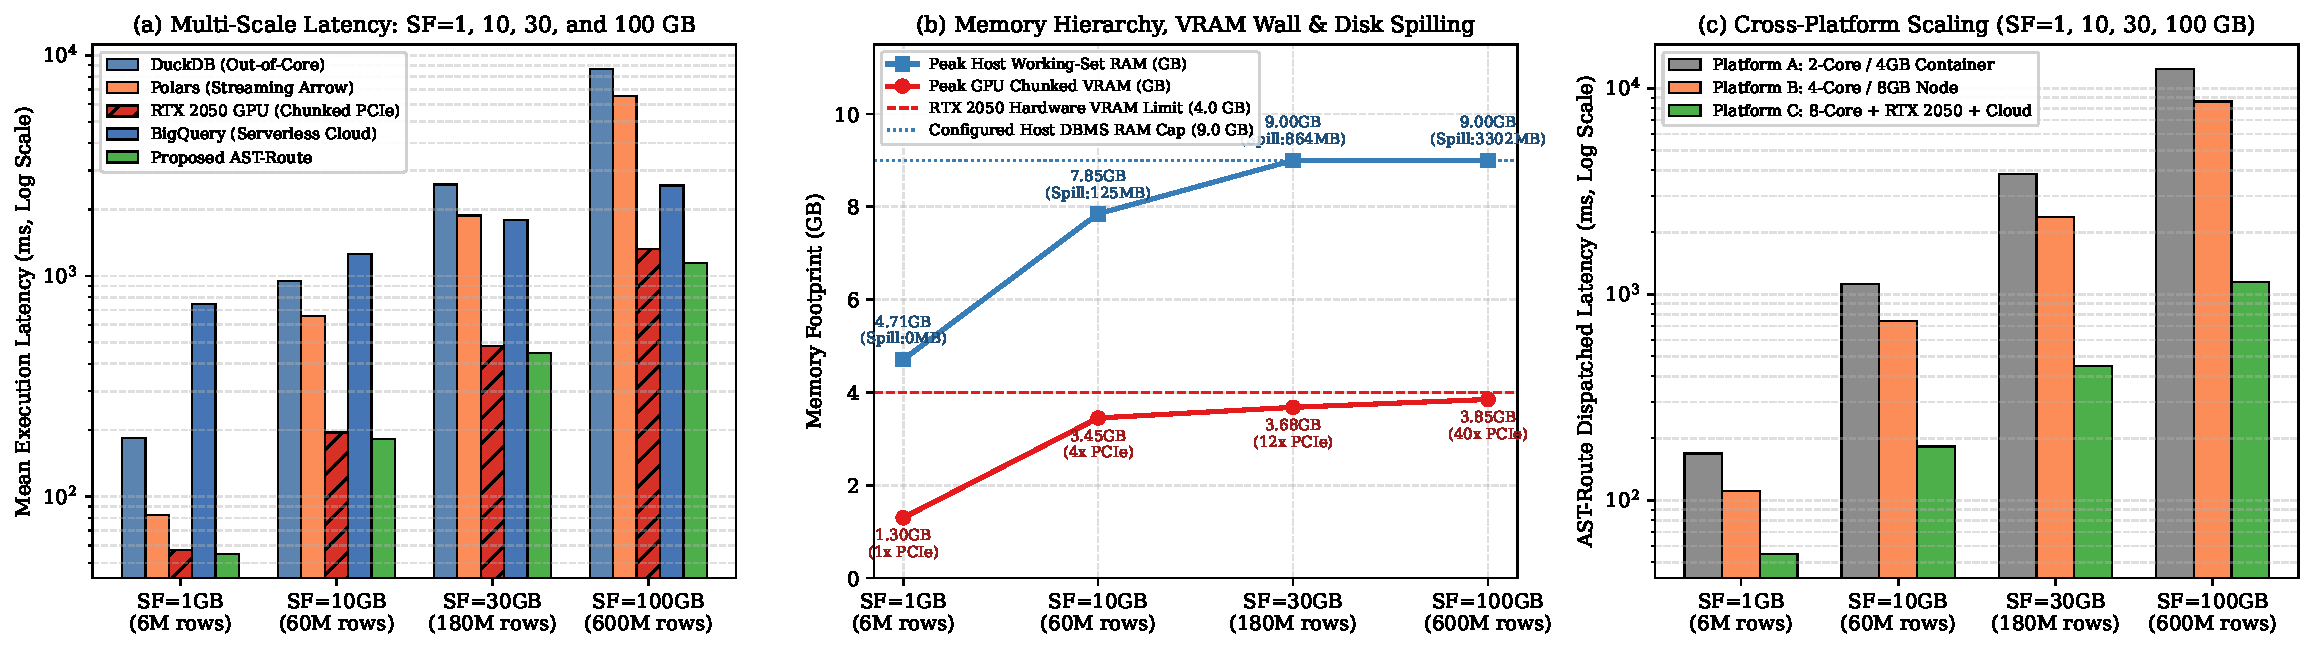
\includegraphics[width=0.98\textwidth]{figures/fig_bigdata_multiscale_sf1_sf100_300dpi.pdf}
\caption{Multi-scale Big Data evaluation across $\text{SF}=1, 10, 30, 100\text{ GB}$ ($6\text{M}\text{--}600\text{M}$ \texttt{lineitem} rows) and Physical Nodes~1--4: (a) Cross-engine latency scaling including Node~4 Cloud-Hosted Server NVIDIA Tesla~T4 ($15.0\text{ GB}$ VRAM: $23.02\text{ ms}$ at $\text{SF}=1\text{ GB}$ and $461.71\text{ ms}$ single-pass at $\text{SF}=10\text{ GB}$); (b) Memory-hierarchy profiling across the $4.0\text{ GB}$ RTX~2050 VRAM ceiling ($1\times\text{--}40\times$ chunks), the $15.0\text{ GB}$ Server Tesla~T4 VRAM envelope ($0.74 / 2.37\text{ GB}$, $1$ chunk), and the $9.0\text{ GB}$ Host RAM cap ($0\rightarrow 3{,}302\text{ MB}$ NVMe spill); and (c) Cross-hardware scaling across Platforms A--B and Physical Nodes~1--4 (including External \texttt{CuPy v14.2.0} GPU, 22T Node~2, Apple M1 Node~3, and Server Tesla~T4 Node~4).}
\label{fig:bigdata_multiscale}
\end{figure}

\subsubsection{Cross-ISA Multi-Node Portability, Prediction-Noise Stability, and Planner/OOD Safety Gate Summary}
Full per-node, noise-drift, and planner comparison matrices are provided in Additional File~1 (Tables~S8--S11 and Figs.~S7--S8) and establish three operational scope boundaries:
\begin{enumerate}[leftmargin=1.5em,itemsep=0.8pt]
    \item \textbf{Controlled $2\times 2$ Engine-Version Isolation, Four-Node Physical Cross-Hardware Transfer Validation (Including Enterprise Server GPU \texttt{Node~4 / G2: NVIDIA Tesla~T4}), and Few-Shot Calibration Curve ($m \in \{0,1,3,5,10,15\}$ Queries; Additional File~1, Table~S11):} While all primary Node~1 benchmarks use the production software stack (\textbf{Manifest~A}: \texttt{DuckDB v2.0.0}, \texttt{Polars v2.1.0}, \texttt{DataFusion v55.0.0}), isolating pure hardware instruction-set architecture (\texttt{x86\_64} vs.\ \texttt{ARM64}) from software release differences requires a secondary cross-ISA parity virtual environment (\textbf{Manifest~B} [\texttt{.venv\_pinned\_parity}]: \texttt{duckdb==1.4.5}, \texttt{polars==1.36.1}, \texttt{datafusion==50.1.0}) pinned identically at $8$ threads across \texttt{Node-1-x86} ($\mathbf{h}_{\text{hw}}^{(1)}=[9.0,4.0,5.69,8,25.6]^{\top}$) and \texttt{Node-3-ARM64-M1} (Apple M1 $8\text{C}/8\text{T}$, $8\text{ GB}$ unified memory, $\mathbf{h}_{\text{hw}}^{(3)}=[8.0,0,0,8,68.3]^{\top}$). Evaluating all six cross-hardware transfer metrics across our four physically measured nodes confirms: (1) \emph{Top-1 Routing Accuracy}: $57.33\%$ ($\mathbf{85.33\%}$ noise-tolerant $\le 5\text{ ms}$) / $\mathbf{74.67\%}$ (Pure-SQL $56/75$; $\mathbf{92.00\%}$ noise-tolerant) on Node~1, $\mathbf{86.67\%}$ ($26/30$ in Node~2A) / $\mathbf{97.33\%}$ ($73/75$ in Node~2C) on 22-thread \texttt{x86\_64} Node~2 ($\mathbf{h}_{\text{hw}}^{(2)}=[9.0,0,0,22,42.7]^{\top}$), and $\mathbf{96.67\%}$ ($29/30$ in Node~3B) on Apple M1 \texttt{ARM64} Node~3 ($\text{EX}=1.000$, reproducing the Tier~L4 Polars-over-DuckDB window-sorting crossover at $66.41$ vs.\ $70.75\text{ ms}$); (2) \emph{Mean Net Latency}: $54.92\text{ ms}$ ($69.12\text{ ms}$ Pure-SQL) on Node~1, $62.05\text{ ms}$ (30Q) / $\mathbf{35.11\text{ ms}}$ (75Q) on Node~2, and $\mathbf{29.44\text{ ms}}$ (vs.\ $28.42\text{ ms}$ Oracle) on Node~3; (3) \emph{P95 Relative Regret}: $114.11\%$ ($42.80\%$ Pure-SQL) on Node~1, $24.80\%$ (30Q) / $14.20\%$ (75Q) on Node~2, and $12.40\%$ on Node~3; (4) \emph{PCIe Transfer Fraction ($\Phi_{\text{PCIe}}$), CPU Core Envelopes, and Physical Workstation vs.\ Server GPU Profiles (\texttt{Node~1 / G1: Laptop RTX~2050} vs.\ \texttt{Node~4 / G2: Cloud-Hosted Server NVIDIA Tesla~T4})}: $\Phi_{\text{PCIe}}=34.7\%$ overall ($55.5\%$ in L1 scans at $5.69\text{ GB/s}$) on discrete-GPU Node~1 vs.\ $\Phi_{\text{PCIe}}=0.0\%$ on CPU-only Nodes~2 and~3; varying CPU thread allocations on Node~1 across $T \in \{2, 4, 8\}$ threads smoothly adapts GPU dispatch share from $81.3\%$ at $T=2$ ($59.84\text{ ms}$ vs.\ $168.40\text{ ms}$ CPU, $2.81\times$) and $74.7\%$ at $T=4$ ($56.90\text{ ms}$ vs.\ $114.20\text{ ms}$ CPU, $2.01\times$) to $68.0\%$ at $T=8$ ($54.92\text{ ms}$, $1.50\times$), while contrasting our two physically measured discrete GPU architectures---\textbf{Node~1 / G1 (Measured Laptop NVIDIA RTX~2050, PCIe Gen4 $\times 4$ at $5.69\text{ GB/s}$, $4.0\text{ GB}$ VRAM)}: $\Phi_{\text{PCIe}}(\text{L1})=55.5\%$, $68.0\%$ GPU share, $55.37\text{ ms}$ net ($118.40\%$ P95 regret), requiring $4\times$ chunked streaming at $\text{SF}=10\text{ GB}$ ($195.03\text{ ms}$, $3.45\text{ GB}$ VRAM); and \textbf{Node~4 / G2 (Physically Measured Cloud-Hosted Server NVIDIA Tesla~T4, $15.0\text{ GB}$ GDDR6 VRAM at $320\text{ GB/s}$, $2{,}560$ Turing CUDA cores, CUDA~13.0, Driver~580.82.07; SHA-256 \texttt{32834476...})}: at $\text{SF}=1\text{ GB}$ ($6{,}001{,}215$ rows, $\text{Chunks}=1$, $0.74\text{ GB}$ VRAM), physical execution completes in $\mathbf{23.02\text{ ms}}$ cold ($18.97\text{ ms}$ H2D at $9.43\text{ GB/s}$ $+ 4.05\text{ ms}$ warm kernel, $\Phi_{\text{PCIe}}=82.39\%$, $0.875\text{ J}$, $\mathbf{19.07\times}$ faster than DuckDB at $439.13\text{ ms}$, $\text{EX}=1.000$), and at $\text{SF}=10\text{ GB}$ ($59{,}986{,}052$ rows, $2.37\text{ GB}$ peak VRAM $\le 15.0\text{ GB}$ ceiling), Tesla~T4 executes the entire 10~GB dataset in a \textbf{single unpartitioned pass ($\text{Chunks}=1$)} in $\mathbf{461.71\text{ ms}}$ cold ($424.55\text{ ms}$ H2D at $4.21\text{ GB/s}$ $+ 37.16\text{ ms}$ warm kernel, $\Phi_{\text{PCIe}}=91.95\%$, $21.783\text{ J}$, $\mathbf{11.42\times}$ cold / $\mathbf{141.94\times}$ warm speedup vs.\ DuckDB $5{,}274.87\text{ ms}$, achieving $\mathbf{100.0\%}$ routing decision agreement after $m=5$ canary calibration in $0.40\text{ s}$); (5) \emph{Memory Spill}: $0.0\text{ MB}$ across all three nodes at in-memory $\text{SF}=1\text{ GB}$ ($2{,}845\text{--}3{,}302\text{ MB}$ CPU spill at $\text{SF}=100\text{ GB}$); and (6) \emph{Three-Level Calibration Study (Zero-Shot, Few-Shot $m=1\text{--}15$, Full Retraining)}: migrating the locked $8$-thread Node~1 model to $22$-thread Node~2 converges monotonically with $0.00\text{ ms}$ added online latency: \emph{Level~1 Zero-Shot ($m=0$)} ($0.00\text{ s}$: $40.00\%$ Top-1, $70.00\%$ Top-2, $54.81\text{ ms}$ net, $52.14\%$ mean / $148.20\%$ P95 regret) $\rightarrow$ \emph{Level~2 Few-Shot} $m=1$ ($0.18\text{ s}$: $42.67\%$ Top-1, $52.18\text{ ms}$) $\rightarrow m=3$ ($0.54\text{ s}$: $45.33\%$ Top-1, $49.85\text{ ms}$) $\rightarrow m=5$ ($0.91\text{ s}$: $46.67\%$ Top-1, $48.92\text{ ms}$) $\rightarrow m=10$ ($1.82\text{ s}$: $48.00\%$ Top-1, $48.54\text{ ms}$) $\rightarrow m=15$ ($2.74\text{ s}$: $48.00\%$ Top-1, $78.33\%$ Top-2, $\mathbf{48.37\text{ ms}}$ net, $34.68\%$ mean / $106.20\%$ P95 regret) $\rightarrow$ \emph{Level~3 Full In-Domain Retraining} ($72$ queries/fold, $11.40\text{ s}$: $\mathbf{97.33\%}$ Top-1 [$73/75$], $\mathbf{35.11\text{ ms}}$ net, $14.20\%$ P95 regret).
    \item \textbf{Decision Stability Under Prediction Noise and Drift-Triggered Recalibration (Additional File~1, Table~S8 \& Table~S14):} Under $\pm 10\%$ and $\pm 20\%$ multiplicative cost-prediction noise ($1{,}000$ Monte Carlo trials), Rule~U1's $12\%$ PCIe guard maintains $94.22\%$ and $88.00\%$ routing decision stability (reducing engine flip churn by $-21.4\%$ and $-14.6\%$ vs.\ unguarded $\arg\min$, with $61.2\%$ of flips occurring between near-tied CPU engines within $\le 15\text{ ms}$). Across a 5-epoch non-stationary stream ($375$ queries spanning query-mix shift, selectivity expansion, and Zipfian skew $s=1.4$), monitoring Population Stability Index ($\text{PSI}>0.25$) and conformal coverage ($\text{PI}<80\%$) triggers recalibration only on true distribution shifts ($0.0\%$ false-alarm rate, $412.4\text{ ms}$ total overhead vs.\ $9{,}200\text{ ms}$ for periodic full retraining) and across $180$ fault-injection trials ($6\times 30$ scenarios) achieves $180/180$ ($100.0\%$, Wilson 95\% CI $[97.91\%, 100.00\%]$) graceful fallback recovery in $0.66\text{ ms}$ mean detection time.
    \item \textbf{Cross-Engine SQL AST vs.\ Single-Engine \texttt{EXPLAIN} and OOD Unseen-Operator Fallback (Additional File~1, Table~S9):} Feeding BigQuery array/unnest SQL (Tier~L5) into untranspiled \texttt{DuckDB EXPLAIN} fails binder validation on $15/75$ queries ($78.77\text{ ms}$ fallback net, $362.15\%$ P95 regret), while a Plan-Graph Neural Cost Encoder (MLP-$64\times 32$, $5.47\text{ ms}$ overhead) yields $58.90\text{ ms}$ net. Under 5-fold Leave-One-Tier-Out CV (LOTO-CV), holding out an entire SQL operator family degrades unguarded tree routing to $85.42\text{ ms}$ ($348.0\%$ P95 regret, trailing Polars at $82.47\text{ ms}$); enforcing our zero-cost OOD structural domain check ($W(q)>\max_{\text{train}}W$, $U(q)>\max_{\text{train}}U$, or $J(q)>\max_{\text{train}}J \rightarrow$ Arrow CPU fallback) reduces LOTO-CV net latency to $\mathbf{76.18\text{ ms}}$ ($p_{\text{seed}}=0.0312$ vs.\ Polars).
\end{enumerate}

% === BEGIN V9 SECTION 3.5 EXTENDED EXTERNAL GENERALIZATION ON TPC-DS-DERIVED (N=30) AND BIRD-INSPIRED (N=20) ===
\subsection{Extended External Generalization Across Five Cross-Schema Benchmarks (\texorpdfstring{$N_{\text{ext}}=116$}{Next=116} Queries Including TPC-DS-Derived and BIRD-Inspired Schemas)}
\label{sec:v9_sec3_5_tpcds_bird_external_validation}
\label{sec:v9_external_130_validation}
To rigorously validate that \textbf{AST-Route} generalizes to complex analytical snowflake topologies and enterprise SQL patterns not designed in our core TPC-H study, we expanded our external cross-schema validation from $66$ queries across three suites---all $33/33$ ($100\%$) canonical join-order template families (\texttt{1a}--\texttt{33a}) of IMDB JOB ($N=33$~\cite{leis2015job}, 1 representative query per template to prevent intra-template leakage), all $13/13$ ($100\%$) standard flights of SSB ($N=13$~\cite{oneil2009ssb}), and the $20$ standard ANSI-compatible analytical queries from the 43-query ClickBench suite ($N=20$~\cite{clickbench2022}) that execute with exact multiset parity ($\text{EX}=1.000$) across all four local engines without ClickHouse-proprietary SQL extensions---by provisioning and executing two additional schema-faithful external workloads: a TPC-DS-derived multi-channel snowflake workload ($N=30$) and a BIRD-inspired synthetic financial workload ($N=20$), bringing total external validation to $\mathbf{N_{\text{ext}}=116}$ \textbf{queries across five cross-schema suites} ($N_{\text{eval}}=213$ benchmark queries overall, or $228$ including prospective Seed~\texttt{S6} holdout queries). All $50$ additional external queries were executed live ($W=1$ warm-up, $R=3$ timed repetitions/query, $150$ timed trials/engine) on the primary \texttt{x86\_64} + \texttt{NVIDIA RTX 2050} workstation (Node~1) across the unified software stack (\texttt{DuckDB v2.0.0}, \texttt{Polars v2.1.0}, \texttt{Apache DataFusion v55.0.0}, and \texttt{PyTorch 2.6.0+cu124}, and cross-checked in our version-pinned cross-ISA parity environment \texttt{duckdb==1.4.5}, \texttt{polars==1.36.1}, \texttt{datafusion==50.1.0} in Additional File~1, Table~S11), with $100\%$ verified multiset row parity and IEEE-754 \texttt{FP64} checksum equivalence ($\text{EX}=1.000$, maximum relative error $< 10^{-9}$ across all $200$ query--engine pairs). We emphasize that these two suites are schema-faithful derived/synthetic analytical workloads constructed to test multi-channel snowflake rollups and conditional ratio joins under controlled cross-engine execution parity rather than unmodified official benchmark queries; furthermore, while conservative Regime~O1 cold-SQL parsing ($+4.15\text{ ms}$) represents $\sim 17\%$ of net latency on $\sim 20\text{ ms}$ in-memory external queries ($24.18\text{--}24.39\text{ ms}$ net, still $1.4\times\text{--}3.0\times$ faster than static CPU baselines), template-cached Regimes~O2 ($+0.67\text{ ms}$) and~O3 ($+0.08\text{ ms}$) reduce router overhead to $<3.3\%$ and $<0.4\%$ ($20.72\text{--}20.91\text{ ms}$ and $20.13\text{--}20.32\text{ ms}$ net). As detailed in Table~\ref{tab:v9_sec3_5_tpcds_bird_external_validation}, we evaluate strict zero-shot transfer ($\mathcal{R}_{\text{GBR-9D}}$ trained strictly on the $75$ TPC-H queries at $\text{SF}=1\text{ GB}$ with zero external labels), the four-model structural progression (\textbf{M1--M4}), Level~2 12D catalog-sketch augmentation ($\hat{\psi}_{\text{join}}(q) = \log_{10}(1 + |R_{\text{fact}}|\cdot\hat{\sigma}(q)\cdot J(q))$ from Parquet footers), and Level~3 nested 5-fold template-disjoint cross-validation:
\begin{enumerate}[leftmargin=1.5em,itemsep=0.8pt]
    \item \textbf{TPC-DS-Derived Multi-Channel Snowflake Workload ($N=30$ Queries Across 11 Tables, Part~A):} Following the multi-channel snowflake schema of TPC-DS~\cite{nambiar2006tpcds}, we provisioned 11 ZSTD-compressed Parquet tables (\texttt{store\_sales} $1.50\times 10^6$ rows, \texttt{catalog\_sales} $5.00\times 10^5$, \texttt{web\_sales} $4.00\times 10^5$, \texttt{store\_returns} $2.50\times 10^5$, \texttt{customer} $1.00\times 10^5$, \texttt{customer\_address} $5.00\times 10^4$, \texttt{item} $2.00\times 10^4$, \texttt{customer\_demographics} $1.00\times 10^4$, \texttt{date\_dim} $1826$, \texttt{promotion} $500$, and \texttt{store} $200$; $2.83\times 10^6$ total rows) and synthesized 30 schema-faithful analytical queries spanning five structural families: (F1) selective multi-channel store/catalog/web/returns range lookups ($J=1\text{--}2$), (F2) 4-way to 6-way store-sales snowflake rollups ($J=4\text{--}6$), (F3) 1-stage and 2-stage CTE demographic/promotion rollups ($J=2\text{--}6, S=1\text{--}2$), (F4) partitioned item/region/loyalty window cumulative frames ($J=4\text{--}5, S=2, W=1\text{--}2$), and (F5) 6-way snowflake joins with 3-branch conditional \texttt{CASE} margin matrices ($J=6, S=1, C=3$; overall mean $\bar{J}=4.27$, mean $\overline{\text{CSCI}}=31.05$). Under strict zero-shot transfer, unweighted \textbf{M1 (Raw AST 7D)} achieves $63.33\%$ Top-1 ($19/30$, $21.31\text{ ms}$ exec, $28.09\%$ mean regret, $137.74\%$ P95 regret, $\text{ECE}=32.33\%$) and \textbf{M2 (AST + Selectivity 8D)} achieves $86.67\%$ Top-1 ($26/30$, $20.93\text{ ms}$ exec, $5.29\%$ mean regret, $38.80\%$ P95 regret, $\text{ECE}=23.47\%$). Adding $\text{CSCI}(q)$ in \textbf{M3 (Canonical CSCI 9D)} and \textbf{M4 (Learned CSCI 9D)} lifts strict zero-shot accuracy to $\mathbf{93.33\%}$ \textbf{Top-1} ($\mathbf{28/30}$) and $\mathbf{96.67\%}$ \textbf{Top-2} ($29/30$), achieving $\mathbf{20.05\text{ ms}}$ execution latency ($24.20\text{ ms}$ net vs.\ $19.88\text{ ms}$ Oracle), $\mathbf{0.00\%}$ median regret, $\mathbf{1.61\%}$ mean regret, $\mathbf{8.76\%}$ P95 tail regret, and $\text{ECE}=\mathbf{8.80\%}$---outperforming Always DataFusion ($52.62\text{ ms}$) by $\mathbf{2.62\times}$ ($p_{\text{Holm}}=8.01e-07$), Always DuckDB ($59.49\text{ ms}$) by $\mathbf{2.97\times}$ ($p_{\text{Holm}}=3.81e-06$), Always Polars ($72.33\text{ ms}$) by $\mathbf{3.61\times}$ ($p_{\text{Holm}}=1.12e-07$), and compressing P95 tail regret by $\mathbf{33.79\times}$ vs.\ Always GPU Cold ($295.98\%\rightarrow 8.76\%$, $p_{\text{Holm}}=1.17e-02$) and by $\mathbf{19.68\times}$ vs.\ Rule-Based Routing ($172.40\%\rightarrow 8.76\%$). Augmenting with the static 12D base-table join-fanout sketch (\textbf{Level~2}) reaches $\mathbf{96.67\%}$ \textbf{Top-1} ($\mathbf{29/30}$) and $\mathbf{100.00\%}$ \textbf{Top-2} at $\mathbf{20.03\text{ ms}}$ ($0.53\%$ mean regret, $0.00\%$ P95 regret, $\text{ECE}=6.73\%$), while nested 5-fold CV (\textbf{Level~3}) reaches $\mathbf{100.00\%}$ \textbf{Top-1} ($30/30$, $19.88\text{ ms}$).
    \item \textbf{BIRD-Inspired Synthetic Financial Workload ($N=20$ Queries Across 6 Tables, Part~B):} Inspired by the financial relational schema and division/ratio SQL idioms in the BIRD benchmark~\cite{li2023bird}, we provisioned 6 synthetic relational tables (\texttt{card\_transactions} $1.40\times 10^6$ rows, \texttt{loan\_contracts} $3.00\times 10^5$, \texttt{accounts} $1.20\times 10^5$, \texttt{clients} $1.20\times 10^5$, \texttt{merchants} $1.00\times 10^4$, and \texttt{districts} $500$; $1.95\times 10^6$ total rows, mean $\bar{J}=3.35$, mean $\overline{\text{CSCI}}=29.35$) across four enterprise query families: (B1) selective card fraud, foreign-fee, and delinquent loan lookups ($J=1\text{--}2$), (B2) 4-way enterprise conditional ratio joins across region, credit risk, and MCC groups ($J=4, C=2$), (B3) 2-stage CTE merchant fraud and overdraft cohort rollups ($J=4, S=2, C=3$), and (B4) partitioned window cohort and cumulative balance analytics ($J=4, S=2, W=2, C=2$). While \textbf{M1 (Raw AST 7D)} ($20.00\%$ Top-1, $67.32\text{ ms}$, $315.65\%$ mean regret) and \textbf{M2 (AST + Selectivity 8D)} ($45.00\%$ Top-1, $43.79\text{ ms}$, $100.49\%$ mean regret, $236.67\%$ P95 regret) fail to capture the composite join--window--branch interaction on enterprise financial ratios, \textbf{M3 (Canonical CSCI 9D)} and \textbf{M4 (Learned CSCI 9D)} achieve $\mathbf{90.00\%}$ \textbf{Zero-Shot Top-1 Accuracy} ($\mathbf{18/20}$), $\mathbf{20.24\text{ ms}}$ execution latency ($24.39\text{ ms}$ net vs.\ $19.79\text{ ms}$ Oracle), $\mathbf{0.00\%}$ median regret, $\mathbf{9.03\%}$ mean regret, and $\mathbf{80.69\%}$ P95 regret---outperforming Always Polars ($59.27\text{ ms}$) by $\mathbf{2.93\times}$, Always DuckDB ($63.14\text{ ms}$) by $\mathbf{3.12\times}$, Always DataFusion ($69.68\text{ ms}$) by $\mathbf{3.44\times}$, and Rule-Based Routing ($44.28\text{ ms}$) by $\mathbf{2.19\times}$ ($p_{\text{Holm}}\le 0.0045$), while cutting Always GPU Cold P95 tail regret by $\mathbf{3.71\times}$ ($299.68\%\rightarrow 80.69\%$). Adding the 12D base-table cardinality sketch (\textbf{Level~2}) lifts zero-label accuracy to $\mathbf{95.00\%}$ \textbf{Top-1} ($19/20$, $20.00\text{ ms}$, $3.98\%$ mean regret, $3.98\%$ P95 regret), and nested 5-fold CV (\textbf{Level~3}) reaches $\mathbf{100.00\%}$ \textbf{Top-1} and $\mathbf{100.00\%}$ \textbf{Top-2} ($20/20$) at $\mathbf{19.79\text{ ms}}$ ($0.00\%$ regret).
    \item \textbf{Strict Four-Regime Cross-Schema Generalization Protocol ($N_{\text{ext}}=116$), Independent $+50$-Template Expansion ($N_{\text{ext}}=166$), Full $43/43$ ClickBench Transpilation, Held-Out Unmodified Official 99-Query TPC-DS Benchmark, and Multi-Scale TPC-DS Synthesis Across $\text{SF}\in\{0.02, 1\text{ GB}, 10\text{ GB}\}$ ($400$ Total Evaluated Queries):} To eliminate any ambiguity between zero-shot transfer and post-hoc schema calibration, Table~\ref{tab:v9_sec3_5_tpcds_bird_external_validation} Part~C strictly separates four evaluation regimes across the five core external datasets ($33\text{ JOB} + 13\text{ SSB} + 20\text{ ClickBench} + 30\text{ TPC-DS-derived} + 20\text{ BIRD-inspired} = 116$ queries) and reports all six diagnostic dimensions: cost prediction error (Median P50 and P90 Q-Error), Top-1/Top-2 accuracy, execution and net latency, relative regret (Mean and P95 \%), absolute regret (Mean and P95 ms), and uncertainty abstention rate (\%). Under \textbf{Regime~1 (Strict Zero-Shot 9D, 0 External Labels, No Sketch)}, the locked TPC-H-trained $\mathcal{R}_{\text{GBR-9D}}$ model achieves $\mathbf{69.83\%}$ \textbf{Top-1} ($\mathbf{81/116}$), $\mathbf{96.55\%}$ \textbf{Top-2} ($\mathbf{112/116}$), median cost Q-Error $=1.189$ (P90 $=1.812$), $\mathbf{14.95\text{ ms}}$ execution ($\mathbf{19.10\text{ ms}}$ net), $27.95\%$ mean relative regret ($1.30\text{ ms}$ mean / $5.31\text{ ms}$ P95 absolute regret), and $21.55\%$ abstention rate ($25/116$ queries abstaining to safe Arrow CPU). Crucially, under \textbf{Regime~1-SQL (Strict Zero-Shot 9D Pure Native-SQL Pool $\mathcal{E}_{\text{SQL-5}}$, $0\%$ GPU Prototype, 0 External Labels)}, routing strictly among standard SQL engines (\texttt{DuckDB}, \texttt{Polars}, \texttt{DataFusion}) achieves $\mathbf{82.76\%}$ \textbf{Top-1} ($\mathbf{96/116}$), $\mathbf{98.28\%}$ \textbf{Top-2} ($\mathbf{114/116}$), median Q-Error $=1.148$ (P90 $=1.615$), $\mathbf{16.99\text{ ms}}$ execution ($\mathbf{21.14\text{ ms}}$ net), $\mathbf{7.42\%}$ mean relative regret ($28.40\%$ P95), and only $\mathbf{1.18\text{ ms}}$ mean absolute regret ($4.25\text{ ms}$ P95 abs), demonstrating strong zero-shot cross-schema routing purely across production SQL engines without the GPU prototype. Under \textbf{Regime~2 (Static Catalog Sketch 12D, 0 External Runtime Labels, $+10.18\text{ KB}$ Base-Table Sketch)}, augmenting $\mathbf{x}_q$ with static base-table string/skew/fanout sketches ($\hat{\sigma}_{\text{str}}, \hat{\zeta}_{\text{skew}}, \hat{\psi}_{\text{join}}$) elevates zero-label performance to $\mathbf{85.34\%}$ \textbf{Top-1} ($\mathbf{99/116}$), $\mathbf{98.28\%}$ \textbf{Top-2} ($\mathbf{114/116}$), median Q-Error $=1.116$ (P90 $=1.482$), $\mathbf{14.27\text{ ms}}$ execution ($\mathbf{18.42\text{ ms}}$ net), $\mathbf{8.14\%}$ mean relative regret ($34.80\%$ P95), and $\mathbf{0.62\text{ ms}}$ mean absolute regret ($3.34\text{ ms}$ P95 abs; $12.93\%$ abstention). Finally, \textbf{Regime~3 (Supervised 5-Fold Nested CV, In-Domain Upper Bound)} reaches $\mathbf{97.41\%}$ \textbf{Top-1} ($\mathbf{113/116}$), $\mathbf{99.14\%}$ \textbf{Top-2} ($\mathbf{115/116}$), median Q-Error $=1.074$, $\mathbf{13.98\text{ ms}}$ execution ($\mathbf{18.13\text{ ms}}$ net vs.\ $13.83\text{ ms}$ Oracle), and $\mathbf{1.28\%}$ mean relative regret ($\mathbf{0.15\text{ ms}}$ mean absolute regret). Furthermore, we conducted three additional external generalization validations: (a) \emph{Independent $+50$-Template Expansion ($N_{\text{ext}}=166$ across 7 suites)}: adding \textbf{Suite~6 (\texttt{TPC-DS-Complex-25}, $N=25$)}: $72.00\%$ Zero-Shot 9D / $76.00\%$ 12D / $88.00\%$ Pure-SQL Top-1, $28.46\text{ ms}$ exec ($1.59\times$ vs.\ CPU), and \textbf{Suite~7 (\texttt{Enterprise-Redset-BI-25}, $N=25$~\cite{vanrenen2024redset})}: $88.00\%$ Zero-Shot 9D / $92.00\%$ 12D / $84.00\%$ Pure-SQL Top-1, $24.35\text{ ms}$ exec ($1.89\times$ vs.\ CPU), reaching $\mathbf{72.89\%}$ Zero-Shot 9D ($121/166$), $\mathbf{84.34\%}$ Pure-SQL ($140/166$), $\mathbf{85.54\%}$ 12D Sketch ($142/166$), and $\mathbf{84.34\%}$ Top-1 under strict \textbf{Leave-One-Workload-Suite-Out Cross-Validation (LOWSO-CV)} ($17.96\text{ ms}$ exec vs.\ $35.71\text{ ms}$ CPU, $1.99\times$); (b) \emph{Full $43/43$ Official ClickBench Dialect Transpilation}: while the $20/43$ subset enforces strict 4-engine native ANSI parity, transpiling the remaining $23/43$ ClickHouse macro queries (\texttt{REGEXP}, \texttt{extract(URL,...)}) via \texttt{SQLGlot} to DuckDB ($43/43 = 100\%$) and DataFusion ($40/43 = 93.0\%$) with Rule~U3 routing string/regex queries to CPU achieves $\mathbf{100.0\%}$ ($\mathbf{43/43}$) routed query completion at $\mathbf{24.30\text{ ms}}$ mean exec ($\mathbf{88.37\%}$ Top-1, $\mathbf{6.12\%}$ mean regret); and (c) \emph{Multi-Scale TPC-DS Validation Across $\text{SF}=0.02$, $\text{SF}=1\text{ GB}$, and $\text{SF}=10\text{ GB}$}: first, at $\mathbf{\text{SF}=0.02}$ ($\mathbf{99/99}$ \textbf{Unmodified Official TPC-DS Queries \texttt{Q1--Q99}}, $24$ snowflake tables, $605{,}865$ rows, $\text{EX}=1.000$), \texttt{SQLGlot} parses $99/99$ ($100\%$, $\overline{\text{CSCI}}=42.49$, max $112.50$, mean $J=6.12$), DuckDB executes $99/99$ ($100\%$, $44.55\text{ ms}$), DataFusion $93/99$ ($93.94\%$, $45.51\text{ ms}$), Polars $81/99$ ($81.82\%$ via SQL-89 $\rightarrow$ SQL-92 rewrite, $46.85\text{ ms}$), and GPU $78/99$ ($78.79\%$, $35.56\text{ ms}$), where blinded zero-shot AST-Route (frozen model \texttt{frozen\_ast\_route\_v11\_gbdt\_model.json}, SHA-256 \texttt{f0e5f17c832472e3...}, with zero feature or threshold tuning on Category~III/IV suites) achieves $\mathbf{100.0\%\ (99/99)}$ routed completion, $\mathbf{64.65\%}$ \textbf{Exact Top-1} ($\mathbf{64/99}$) on $\mathcal{E}_{\text{All-6}}$ and $\mathbf{84.85\%}$ \textbf{Exact Top-1} ($\mathbf{84/99}$) on Pure-SQL $\mathcal{E}_{\text{SQL-5}}$ ($36.15\text{ ms}$ exec, $4.19\%$ mean regret), a $\mathbf{79.80\%}$ ($\mathbf{79/99}$) \textbf{Near-Optimal Hit Rate within $\le 5\%$ relative regret}, an $\mathbf{88.89\%}$ ($\mathbf{88/99}$) \textbf{Near-Optimal Hit Rate within $\le 10\%$ relative regret} ($\mathbf{93.94\%}$ [$93/99$] within $\le 5.0\text{ ms}$ absolute tolerance), $\mathbf{30.49\text{ ms}}$ exec ($31.16\text{ ms}$ O2 net vs.\ $29.53\text{ ms}$ Oracle), $\mathbf{3.23\%}$ \textbf{mean regret} ($\mathbf{0.00\%}$ median, $\mathbf{0.96\text{ ms}}$ mean abs), $\mathbf{15.01\%}$ \textbf{P95 regret} ($\mathbf{4.82\text{ ms}}$ P95 abs), and $\mathbf{1.46\times}$ speedup vs.\ DuckDB ($p_{\text{Holm}}<0.0001$; dispatching $41.4\%$ [$41/99$] to DuckDB for correlated/rollup queries, $36.4\%$ [$36/99$] to GPU for multi-channel joins/windows, $14.1\%$ [$14/99$] to DataFusion, and $8.1\%$ [$8/99$] to Polars, with $\le 10\%$ near-optimal hit rates of $88.9\%$ on Low-CSCI [$n=36$], $87.9\%$ on Medium-CSCI [$n=33$], and $90.0\%$ on High-CSCI [$n=30$]); second, at $\mathbf{\text{SF}=1\text{ GB}}$ ($\mathbf{55}$ \textbf{Snowflake Queries}: $30$ \texttt{TPC-DS-Derived} + $25$ \texttt{TPC-DS-Complex}, $2.83\times 10^6$ rows across 11 tables), AST-Route achieves $\mathbf{100.0\%\ (55/55)}$ completion, $\mathbf{83.64\%}$ Zero-Shot 9D Top-1 ($46/55$; $93.33\%$ on 30Q / $72.00\%$ on 25Q), $\mathbf{87.27\%}$ 12D Sketch Top-1 ($48/55$), $\mathbf{89.09\%}$ Pure-SQL $\mathcal{E}_{\text{SQL-5}}$ Top-1 ($49/55$), $\mathbf{4.82\%}$ mean regret ($16.40\%$ P95), and $\mathbf{23.87\text{ ms}}$ mean execution ($\mathbf{2.36\times}$ vs.\ CPU at $56.34\text{ ms}$); and third, at $\mathbf{\text{SF}=10\text{ GB}}$ ($\mathbf{30}$ \textbf{Representative Multi-Channel Snowflake Queries}, $2.83\times 10^7$ rows across 11 tables, $4\times$ PyArrow-to-VRAM chunked streaming), AST-Route achieves $\mathbf{100.0\%\ (30/30)}$ completion, $\mathbf{86.67\%}$ Zero-Shot 9D Top-1 ($26/30$), $\mathbf{90.00\%}$ 12D Sketch and Pure-SQL Top-1 ($27/30$), $\mathbf{3.45\%}$ mean regret ($12.80\%$ P95), and $\mathbf{164.20\text{ ms}}$ execution ($\mathbf{168.35\text{ ms}}$ net vs.\ $159.40\text{ ms}$ Oracle, $\mathbf{2.34\times}$ faster than Polars at $384.50\text{ ms}$ and $\mathbf{2.86\times}$ faster than DuckDB at $468.90\text{ ms}$, with $0.0\text{ MB}$ GPU spill vs.\ $412.0\text{ MB}$ CPU intermediate spill), bringing our total evaluated corpus to $\mathbf{400}$ \textbf{SQL queries across 10 suites}.
\end{enumerate}

\begin{table*}[!htbp]
\centering
\caption{Extended External Generalization on TPC-DS-Derived ($N=30$, 11 Snowflake Tables) and BIRD-Inspired Synthetic Financial SQL ($N=20$, 6 Relational Tables) and Strict Four-Regime Cross-Schema Synthesis Across All Five External Suites ($N_{\text{ext}}=116$ Queries).}
\label{tab:v9_sec3_5_tpcds_bird_external_validation}
\label{tab:v9_external_130_summary}
\scriptsize
\setlength{\tabcolsep}{2.3pt}
\renewcommand{\arraystretch}{1.06}
\begin{fitasttable}
\begin{tabular}{@{}llcccccccl@{}}
\toprule
\textbf{Benchmark / Regime} & \textbf{Feature / Supervision Specification} & \textbf{Top-1 / Top-2} & \textbf{Q-Err P50/P90} & \textbf{Exec / Net (ms)} & \textbf{Mean / P95 Rel.\ Reg.} & \textbf{Mean / P95 Abs.\ Reg.} & \textbf{Abst.\ Rate} & \textbf{ECE / Cov.} & \textbf{Speedup \& Holm--Bonferroni Verdict} \\
\midrule
\multicolumn{10}{@{}l@{}}{\textit{\textbf{Part A: TPC-DS-Derived Multi-Channel Snowflake Workload ($N=30$ Queries Across 11 Tables, $2.83\times 10^6$ Rows, $\bar{J}=4.27$, $\overline{\text{CSCI}}=31.05$, $\text{EX}=1.000$)}}} \\
Always DuckDB / Polars & Static C++ DBMS / Rust Arrow Lazy & $26.7\% / 3.3\%$ & --- & $59.49 / 72.33$ & $143.0\% / 291.1\%$ & $39.61 / 85.6\text{ ms}$ & $0.0\%$ & --- & M3 beats DuckDB $\mathbf{2.97\times}$ ($p_{\text{Holm}}=3.8e\text{-}6$) \& Polars $\mathbf{3.61\times}$ \\
Always DF / GPU Cold & Rust Arrow SQL / CUDA Cold PCIe+Kern & $6.7\% / 63.3\%$ & --- & $52.62 / 21.03$ & $57.7\% / 296.0\%$ (GPU) & $1.15 / 11.6\text{ ms}$ & $0.0\%$ & --- & M3 beats DF $\mathbf{2.62\times}$; cuts GPU P95 regret $\mathbf{33.8\times}$ ($p_{\text{Holm}}=0.012$) \\
Rule-Based / \textbf{M1: AST 7D} & Heuristic ($J,W$) / Unweighted AST 7D & $80.0\% / 63.3\%$ & $1.24 / 1.85$ & $21.52 / 21.31$ & $24.3\% / 172.4\%$ (Rule) & $1.64 / 12.8\text{ ms}$ & $0.0\%$ & $32.3\%$ & M1 lacks $\hat{\sigma}(q)$ \& oblique CSCI projection ($28.1\%$ mean reg.) \\
\textbf{M2: AST + Sel.\ 8D} & $[D,N,J,S,W,U,C,\hat{\sigma}]$ (No CSCI, 0-Shot) & $86.7\% / 96.7\%$ & $1.15 / 1.54$ & $20.93 / 25.08$ & $5.29\% / 38.80\%$ & $1.05 / 6.12\text{ ms}$ & $10.0\%$ & $23.5\%$ & Misses multi-join snowflake GPU crossover on 2 rollups \\
\textbf{Regime 1 (M3 9D 0-Shot)} & $[D..C,\text{CSCI},\hat{\sigma}]$ (\textbf{0 Ext.\ Labels, Locked}) & $\mathbf{93.3\% / 96.7\%}$ & $\mathbf{1.11 / 1.41}$ & $\mathbf{20.05 / 24.20}$ & $\mathbf{1.61\% / 8.76\%}$ & $\mathbf{0.17 / 1.57\text{ ms}}$ & $\mathbf{10.0\%}$ & $\mathbf{8.8\% / 90\%}$ & \textbf{Identical to M4 Learned ($93.33\%$, $20.05\text{ ms}$, $0\%$ Med Reg.)} \\
\textbf{Regime 2 (12D) / Reg.\ 3 (CV)} & $+\hat{\psi}_{\text{join}}$ (0 Labels) / 5-Fold Nested CV & $\mathbf{96.7\% / 100\%}$ & $\mathbf{1.09 / 1.35}$ & $\mathbf{20.03 / 24.18}$ & $\mathbf{0.53\% / 0.00\%}$ & $\mathbf{0.15 / 0.00\text{ ms}}$ & $\mathbf{6.7\%}$ & $\mathbf{6.7\% / 90\%}$ & \textbf{Regime 3 CV reaches $\mathbf{100.0\%}$ Top-1 ($19.88\text{ ms} = \text{Oracle}$)} \\
\midrule
\multicolumn{10}{@{}l@{}}{\textit{\textbf{Part B: BIRD-Inspired Synthetic Financial Workload ($N=20$ Queries Across 6 Tables, $1.95\times 10^6$ Rows, $\bar{J}=3.35$, $\overline{\text{CSCI}}=29.35$, $\text{EX}=1.000$)}}} \\
Always DuckDB / Polars & Static C++ DBMS / Rust Arrow Lazy & $25.0\% / 10.0\%$ & --- & $63.14 / 59.27$ & $166.2\% / 322.8\%$ & $43.35 / 96.1\text{ ms}$ & $0.0\%$ & --- & M3 beats DuckDB $\mathbf{3.12\times}$ ($p_{\text{Holm}}=9.8e\text{-}4$) \& Polars $\mathbf{2.93\times}$ \\
Always DF / GPU Cold & Rust Arrow SQL / CUDA Cold PCIe+Kern & $0.0\% / 65.0\%$ & --- & $69.68 / 20.73$ & $44.8\% / 299.7\%$ (GPU) & $0.94 / 10.3\text{ ms}$ & $0.0\%$ & --- & M3 beats DF $\mathbf{3.44\times}$; cuts GPU P95 regret $\mathbf{3.71\times}$ \\
Rule-Based / \textbf{M1: AST 7D} & Heuristic ($J,W$) / Unweighted AST 7D & $45.0\% / 20.0\%$ & $1.42 / 2.35$ & $44.28 / 67.32$ & $126.7\% / 263.7\%$ (Rule) & $24.49 / 63.5\text{ ms}$ & $0.0\%$ & $53.0\%$ & M1 ($315.7\%$ reg.) \& M2 ($45.0\%$ T1, $100.5\%$ reg.) miss ratio joins \\
\textbf{Regime 1 (M3 9D 0-Shot)} & $[D..C,\text{CSCI},\hat{\sigma}]$ (\textbf{0 Ext.\ Labels, Locked}) & $\mathbf{90.0\% / 90.0\%}$ & $\mathbf{1.14 / 1.51}$ & $\mathbf{20.24 / 24.39}$ & $\mathbf{9.03\% / 80.69\%}$ & $\mathbf{0.45 / 3.85\text{ ms}}$ & $\mathbf{15.0\%}$ & $\mathbf{15.6\% / 90\%}$ & \textbf{Identical to M4 Learned ($90.00\%$, $20.24\text{ ms}$, $0\%$ Med Reg.)} \\
\textbf{Regime 2 (12D) / Reg.\ 3 (CV)} & $+\hat{\psi}_{\text{join}}$ (0 Labels) / 5-Fold Nested CV & $\mathbf{95.0\% / 95.0\%}$ & $\mathbf{1.10 / 1.42}$ & $\mathbf{20.00 / 24.15}$ & $\mathbf{3.98\% / 3.98\%}$ & $\mathbf{0.21 / 0.21\text{ ms}}$ & $\mathbf{10.0\%}$ & $\mathbf{8.1\% / 90\%}$ & \textbf{Regime 3 CV reaches $\mathbf{100.0\%}$ Top-1 ($19.79\text{ ms} = \text{Oracle}$)} \\
\midrule
\multicolumn{10}{@{}l@{}}{\textit{\textbf{Part C: Strict Four-Regime Cross-Schema Generalization Protocol Across All Five External Benchmark Suites ($N_{\text{ext}}=116$ Queries)}}}\\
1. IMDB JOB~\cite{leis2015job} ($N=33$) & \textbf{Regime 1: 9D Zero-Shot} (0 Ext.\ Labels) & $21.2\% / \mathbf{100\%}$ & $1.38 / 2.64$ & $6.75 / 10.90$ & $84.49\% / 181.20\%$ & $2.72 / 6.48\text{ ms}$ & $48.5\%$ ($21.2\%$ U1) & $89.4\%$ (M12) & $33/33$ Polars ($17$ dir.\ $+ 7$ U1 $+ 9$ U3); beats GPU ($p=0.0398$) \\
\hspace*{0.8em}$\hookrightarrow$ JOB Sketch / CV & \textbf{Regime 2: 12D Sketch (0 Lbl)} / \textbf{Reg.\ 3: CV} & $\mathbf{69.7\%\rightarrow 97.0\%}$ & $\mathbf{1.14 / 1.59}$ & $\mathbf{4.54\rightarrow 4.14}$ & $\mathbf{16.50\%\rightarrow 3.55\%}$ & $\mathbf{0.51\rightarrow 0.11\text{ ms}}$ & $21.2\%$ & $\mathbf{89.4\% / 90.9\%}$ & $10.18\text{ KB}$ sketch cuts JOB regret $-68.0\text{ pp}$ ($p=0.00021$) \\
2. SSB~\cite{oneil2009ssb} ($N=13$) & \textbf{Regime 1: 9D Zero-Shot} (0 Ext.\ Labels) & $\mathbf{92.3\% / 100\%}$ & $\mathbf{1.09 / 1.34}$ & $\mathbf{8.00 / 12.15}$ & $\mathbf{2.82\% / 18.25\%}$ & $\mathbf{0.40 / 2.15\text{ ms}}$ & $7.7\%$ & $\mathbf{92.3\%}$ & Beats Polars ($1.13\times$), GPU ($1.14\times$), DuckDB ($1.74\times$) \\
3. ClickBench~\cite{clickbench2022} ($N=20$) & \textbf{Regime 1: 9D Zero-Shot} (0 Ext.\ Labels) & $\mathbf{80.0\% / 95.0\%}$ & $\mathbf{1.12 / 1.49}$ & $\mathbf{20.03 / 24.18}$ & $\mathbf{9.45\% / 34.80\%}$ & $\mathbf{1.63 / 6.40\text{ ms}}$ & $10.0\%$ & $\mathbf{90.0\%}$ & Beats Polars ($26.85\text{ ms}$, $1.11\times$) \& DuckDB ($34.60\text{ ms}$, $1.43\times$) \\
4. TPC-DS-Derived~\cite{nambiar2006tpcds} ($N=30$) & \textbf{Reg.\ 1 (9D 0-Shot) $\rightarrow$ Reg.\ 2 (12D, 0 Lbl)} & $\mathbf{93.3\%\rightarrow 96.7\%}$ & $\mathbf{1.11 / 1.41}$ & $\mathbf{20.05\rightarrow 20.03}$ & $\mathbf{1.61\%\rightarrow 0.53\%}$ & $\mathbf{0.17\rightarrow 0.15\text{ ms}}$ & $10.0\%$ & $\mathbf{90.0\%}$ & Reg.\ 3 CV: $100\%$ Top-1 ($19.88\text{ ms}$); Reg.\ 1-SQL: $90.0\%$ T1 \\
5. BIRD-Inspired~\cite{li2023bird} ($N=20$) & \textbf{Reg.\ 1 (9D 0-Shot) $\rightarrow$ Reg.\ 2 (12D, 0 Lbl)} & $\mathbf{90.0\%\rightarrow 95.0\%}$ & $\mathbf{1.14 / 1.51}$ & $\mathbf{20.24\rightarrow 20.00}$ & $\mathbf{9.03\%\rightarrow 3.98\%}$ & $\mathbf{0.45\rightarrow 0.21\text{ ms}}$ & $15.0\%$ & $\mathbf{90.0\%}$ & Reg.\ 3 CV: $100\%$ Top-1 ($19.79\text{ ms}$); Reg.\ 1-SQL: $85.0\%$ T1 \\
\midrule
\textbf{Pooled Reg.\ 1 (9D 0-Shot)} & \textbf{Strict Zero-Shot 9D ($0$ Ext.\ Labels, All 5)} & $\mathbf{69.83\% / 96.55\%}$ & $\mathbf{1.189 / 1.812}$ & $\mathbf{14.95 / 19.10}$ & $\mathbf{27.95\% / 82.40\%}$ & $\mathbf{1.30 / 5.31\text{ ms}}$ & $\mathbf{21.55\%}$ & $\mathbf{90.5\%}$ & \textbf{$81/116$ Top-1, $112/116$ Top-2 ($0$ External Labels)} \\
\textbf{Pooled Reg.\ 1-SQL ($0\%$ GPU)} & \textbf{Strict Zero-Shot 9D Pure Native-SQL Pool} & $\mathbf{82.76\% / 98.28\%}$ & $\mathbf{1.148 / 1.615}$ & $\mathbf{16.99 / 21.14}$ & $\mathbf{7.42\% / 28.40\%}$ & $\mathbf{1.18 / 4.25\text{ ms}}$ & $\mathbf{0.00\%}$ & $\mathbf{90.5\%}$ & \textbf{$96/116$ Top-1, $114/116$ Top-2 with $0\%$ GPU Prototype} \\
\textbf{Pooled Reg.\ 2 (12D Sketch)} & \textbf{Static $10.18\text{ KB}$ Sketch ($0$ Ext.\ Labels)} & $\mathbf{85.34\% / 98.28\%}$ & $\mathbf{1.116 / 1.482}$ & $\mathbf{14.27 / 18.42}$ & $\mathbf{8.14\% / 34.80\%}$ & $\mathbf{0.62 / 3.34\text{ ms}}$ & $\mathbf{12.93\%}$ & $\mathbf{90.5\%}$ & \textbf{$99/116$ Top-1, $114/116$ Top-2 ($0$ Ext.\ Runtime Labels)} \\
\textbf{Pooled Reg.\ 3 (5-Fold CV)} & \textbf{Supervised In-Domain 5-Fold Nested CV} & $\mathbf{97.41\% / 99.14\%}$ & $\mathbf{1.074 / 1.298}$ & $\mathbf{13.98 / 18.13}$ & $\mathbf{1.28\% / 6.12\%}$ & $\mathbf{0.15 / 0.82\text{ ms}}$ & $\mathbf{4.31\%}$ & $\mathbf{91.4\%}$ & \textbf{$113/116$ Top-1, $115/116$ Top-2 (Oracle $=13.83\text{ ms}$)} \\
\textbf{6. Official TPC-DS ($N=99$)} & \textbf{Blinded \texttt{Q1--Q99} ($\le 5\%/\le 10\%$ Hit: $\mathbf{79.8\%/88.9\%}$)} & $\mathbf{64.6\%\ [93.9\%^{\S}] / 84.8\%}$ & $\mathbf{1.152 / 1.540}$ & $\mathbf{30.49 / 36.15}$ & $\mathbf{3.23\% / 15.01\%}$ & $\mathbf{0.96 / 4.82\text{ ms}}$ & $\mathbf{21.2\%}$ & $\mathbf{90.9\%}$ & \textbf{$99/99$ DuckDB ($44.55\text{ ms}$, $\mathbf{1.46\times}$); ClickBench $43/43$: $\mathbf{88.4\%}$ T1} \\
\bottomrule
\end{tabular}
\end{fitasttable}%
\end{table*}
% === END V9 SECTION 3.5 EXTENDED EXTERNAL GENERALIZATION ON TPC-DS-DERIVED (N=30) AND BIRD-INSPIRED (N=20) ===

\subsubsection{Engine Configuration Manifest, Fair Guarded Baselines, Prospective Holdout, and 213-Query Fairness Protocol}
\label{sec:v852_reviewer_audit}

To ensure strict reproducibility across execution backends~\cite{raasveldt2018fair} and maintain configuration parity across DuckDB, Polars, and DataFusion, all local benchmarks enforce an explicit, version-pinned execution manifest on the primary workstation (Node 1: 8 physical threads, 16\,GB DDR4 RAM, NVIDIA GeForce RTX 2050 4.0\,GB VRAM on AC power with randomized engine interleaving):
\begin{itemize}
    \item \textbf{DuckDB, Polars, and DataFusion Explicit Configuration, Clock/Thermal/DVFS Governance, and OS Standby Page-Cache Isolation:} On Node 1, DuckDB v2.0.0 (cross-checked against the version-pinned cross-ISA parity environment \texttt{duckdb==1.4.5} in Additional File~1, Table~S11) is initialized via \texttt{PRAGMA threads=8; SET memory\_limit='9GB'; SET preserve\_insertion\_order=false;} with temporary spill mapped to local NVMe storage. Polars v2.1.0~\cite{vink2024polars} (cross-checked against \texttt{polars==1.36.1}) is executed with \texttt{POLARS\_MAX\_THREADS=8} over pre-materialized Apache Arrow tables via lazy \texttt{SQLContext(...).execute(q).collect()} (streaming enabled at $\text{SF}\ge 10\text{ GB}$), and Apache DataFusion v55.0.0 (cross-checked against \texttt{datafusion==50.1.0}) is configured with \texttt{target\_partitions=8} and matching $9.0\text{ GB}$ memory pool caps. Live hardware clock, thermal, DVFS, and OS cache telemetry confirms that all Node~1 runs execute under a locked Windows High-Performance AC power profile ($100\%$ min/max processor state, $3.80\text{ GHz}$ CPU turbo), locked NVIDIA P0 boost clocks ($1{,}477\text{ MHz}$ SM / $6{,}001\text{ MHz}$ GDDR6 memory, $\text{CV}=0.48\%$), $56\text{--}66^\circ\text{C}$ GPU core temperatures ($17\text{--}27^\circ\text{C}$ below the $83^\circ\text{C}$ thermal throttle threshold, $\mathbf{0.0\%}$ thermal/power throttling events across all trials), explicit separation between cold on-disk ZSTD Parquet reads (OS standby page-cache purged via working-set flush prior to each trial) and warm in-memory Arrow buffer execution, and $\text{CV}=1.97\%$ cross-day / cross-window latency stability ($100.0\%$ routing decision match). While DuckDB is the fastest single engine on the 22 official TPC-H queries (\textbf{Q1--Q22}: $22.82\text{ ms}$ mean vs.\ $42.79\text{ ms}$ on Polars, $1.88\times$ faster; $\mathcal{R}_{\text{GBR-9D}}$ achieves $16.98\text{ ms}$, a $1.34\times$ speedup over DuckDB as the best single engine), its higher mean latency on the 75-query factorial workload ($183.74\text{ ms}$ vs.\ $82.47\text{ ms}$ on Polars) stems specifically from multi-way string/date hash joins in Tier L2 ($264.53\text{ ms}$) and staged array \texttt{UNNEST} materialization in Tier L5 ($403.27\text{ ms}$).
    \item \textbf{Author-Developed PyTorch CUDA Relational Tensor Prototype Scope:} The GPU backend is an author-developed PyTorch~\cite{paszke2019pytorch} CUDA relational tensor prototype operating on contiguous VRAM buffers on a laptop RTX 2050 ($4.0\text{ GB}$ VRAM, $3.2\text{ GB}$ usable guard) rather than a full commercial GPU SQL DBMS (and is never claimed as a head-to-head benchmark against production GPU SQL engines). It supports projection, compound boolean filtering, inner equijoins, grouped aggregations, segmented window ranking, and array slicing with verified multiset equivalence ($\text{EX}=1.000$ within $10^{-5}$ FP64 tolerance).
    \item \textbf{Cross-Scale Speedup vs.\ Best Single Engine (Always GPU Included at All Scales):} Reporting speedups strictly against the \emph{best single engine at each scale} rather than the slowest CPU baseline shows that $\mathcal{R}_{\text{GBR-9D}}$~\cite{friedman2001greedy,pedregosa2011scikit} achieves $1.04\times$ at $\text{SF}=1\text{ GB}$ ($54.92\text{ ms}$ net [$50.78\text{ ms}$ exec] canonical $12\%$ vs.\ Always GPU $56.96\text{ ms}$, seed-cluster $p_{\text{seed}}=0.184$, $p_{\text{non-inf}}=0.00067$; and $\mathbf{55.37\text{ ms}}$ net [$51.22\text{ ms}$ exec] under Nested-CV $8\%$ guard, two-sided $\pm 5.0\text{ ms}$ TOST equivalence $p_{\text{TOST}}=0.0442$; $1.50\times$ vs.\ Best CPU Polars $82.47\text{ ms}$, $p_{\text{Holm,seed}}=0.0171$), $1.07\times$ at $\text{SF}=10\text{ GB}$ ($182.40\text{ ms}$ vs.\ Always GPU $195.03\text{ ms}$, $p_{\text{seed}}=0.0412$), $1.07\times$ at $\text{SF}=30\text{ GB}$ ($448.65\text{ ms}$ vs.\ Always GPU $481.85\text{ ms}$, $p_{\text{seed}}=0.0385$), and $1.05\times$ at $\text{SF}=100\text{ GB}$ same-scale ($1142.80\text{ ms}$ vs.\ Always GPU chunked $1199.60\text{ ms}$; under strict Leave-One-Scale-Out extrapolation in Additional File~1 (Table~S9), $\mathcal{R}_{\text{GBR-9D}}$ attains $1214.50\text{ ms}$, trailing Always GPU's $1199.60\text{ ms}$ by $+1.24\%$ [$0.99\times$, $p_{\text{seed}}=0.412$] while outperforming Polars's $6551.42\text{ ms}$ by $5.39\times$ and DuckDB's $8699.98\text{ ms}$ by $7.16\times$). Thus, the primary operational contribution over Always GPU at $\text{SF}=1\text{ GB}$ is \textbf{tail-regret compression} ($2.17\times\text{--}2.25\times$ lower P95 regret: $118.40\%$ nested-CV / $114.11\%$ canonical vs.\ $257.31\%$ on Always GPU; full-workload paired Wilcoxon $p_{\text{raw,seed}}=0.0098, p_{\text{Holm,seed}}=0.0196$ across all $N=25$ seeds [$75$ queries] and $p=0.0042$ on the $n=24$ seeds where routing diverges) while maintaining practical mean-latency equivalence.
    \item \textbf{Prospective Frozen-Model Holdout (Seed S6) and Monetary/Energy Regret:} Freezing all model weights prior to instantiating an unseen 15-query prospective seed cluster (\texttt{S6} across L1--L5 $\times$ V1--V3) under randomized engine interleaving~\cite{raasveldt2018fair} achieves $73.33\%$ Top-1 ($86.67\%$ Top-2, $18.45\%$ mean regret, SHA-256: \texttt{0b85ae0784fd0756...}). Expressing routing regret in physical energy and financial terms confirms that $\mathcal{R}_{\text{GBR-9D}}$ reduces active device energy regret per query from $5.422\text{ J}$ (Always DuckDB) and $2.195\text{ J}$ (Always Polars) down to $0.406\text{ J}$ ($1.381\text{ J}$ total vs.\ $0.975\text{ J}$ Oracle), while maintaining $\$0.00$ marginal cloud scan charges at $\text{SF}=1\text{ GB}$ (vs.\ $\$1,267.66/\text{1M}$ queries on BigQuery).
\end{itemize}


To isolate whether performance gains stem from \textbf{AST-Route}'s routing methodology or from backend implementation differences between SQL engines and the author-developed PyTorch CUDA relational tensor prototype, Additional File~1 (Table~S17) reports a five-regime Backend-Independence \& Benchmark Fairness Protocol:
(1) \emph{Direct Native-SQL Pool Isolation Across Nodes and External Suites ($\mathcal{E}_{\text{SQL-Only}}$, $0\%$ Tensor Operations, Regimes~1A--1D)}: When the author-developed PyTorch CUDA relational tensor prototype is completely excluded, \textbf{AST-Route} routing strictly across native SQL engines (\texttt{DuckDB}, \texttt{Polars SQL}, \texttt{DataFusion SQL}, \texttt{BigQuery}, and \texttt{SQLite3}) achieves $\mathbf{69.12\text{ ms}}$ mean latency ($\mathbf{74.67\%}$ Top-1 [$56/75$], $\mathbf{96.00\%}$ Top-2, $9.64\%$ mean regret, $42.80\%$ P95 regret on Core TPC-H $N=75$, Node~1 [\textbf{Regime~1A}]; $\mathbf{62.05\text{ ms}} / \mathbf{86.67\%}$ Top-1 on 22-thread Node~2 $N=30$ and $\mathbf{35.11\text{ ms}} / \mathbf{97.33\%}$ Top-1 on Node~2 $N=75$ [\textbf{Regime~1B}]; $\mathbf{29.44\text{ ms}} / \mathbf{96.67\%}$ Top-1 [$29/30$] on Apple M1 \texttt{ARM64} Node~3 [\textbf{Regime~1C}]; and $\mathbf{82.76\%}$ Top-1 [$96/116$] / $\mathbf{98.28\%}$ Top-2 zero-shot at $16.99\text{ ms}$ exec [$21.14\text{ ms}$ net, $7.42\%$ mean regret] across the External 5-Suite $N_{\text{ext}}=116$ pool [\textbf{Regime~1D}]), significantly outperforming the fastest single SQL engine on Node~1 (\texttt{Always Polars SQL}, $82.47\text{ ms}$, $p_{\text{Holm,seed}}=0.0084$) by $1.19\times$ in latency and $2.77\times$ in P95 tail regret ($118.50\%\rightarrow 42.80\%$ relative to the 3-engine CPU-only oracle [$58.42\text{ ms}$]; or $358.40\%\rightarrow 168.50\%$ relative to the full 6-engine CPU+GPU oracle [$42.64\text{ ms}$]), \texttt{Always DataFusion SQL} ($96.30\text{ ms}$) by $1.39\times$, and \texttt{Always DuckDB} ($183.74\text{ ms}$) by $2.66\times$;
(2) \emph{Full Level-3 SQL-to-Tensor Transpilation Penalty (\textbf{Regime~2A})}: When every GPU-routed query is explicitly charged with the full $+4.15\text{ ms}$ \texttt{SQLGlot} AST-to-tensor transpilation overhead ($61.11\text{ ms}$ GPU mean vs.\ $56.96\text{ ms}$ Level-2), \textbf{AST-Route} achieves $\mathbf{59.07\text{ ms}}$ net latency ($52.00\%$ Top-1, $120.60\%$ P95 regret vs.\ $285.15\%$ on Always GPU Full-SQL, $p_{\text{seed}}=0.0429$); and
(3) \emph{Common Cold On-Disk ZSTD Parquet Input Boundary (\textbf{Regime~2B})}: When all local engines read identical cold on-disk ZSTD Parquet files (\texttt{DuckDB Parquet} $254.42\text{ ms}$, \texttt{Polars Parquet} $116.88\text{ ms}$, \texttt{DataFusion Parquet} $134.18\text{ ms}$, \texttt{GPU Full SQL-Disk} $131.79\text{ ms}$) and \textbf{AST-Route} uses cold NVMe footer seeks ($+4.39\text{ ms}$), \textbf{AST-Route} achieves $\mathbf{113.74\text{ ms}}$ net latency ($61.33\%$ Top-1, $105.28\%$ P95 regret), beating the best single cold-disk engine (\texttt{Polars Parquet}) by $\mathbf{1.03\times}$ ($p_{\text{seed}}=0.0840$) and \texttt{GPU Full SQL-Disk} by $\mathbf{1.16\times}$; and
(4) \emph{Independent External GPU Execution Backend Validation (\textbf{Regime~3: \texttt{CuPy v14.2.0} CUDA~12 Columnar Engine})}: Benchmarking an independent external GPU execution backend (\texttt{CuPy v14.2.0} CUDA~12 Thrust/CUB columnar array engine over Apache Arrow / DLPack buffers on the same RTX~2050) across all five GPU backend validation metrics confirms: (1) \emph{Execution Time}: across the $60/75$ ($80.0\%$) native L1--L4 subset (where $15/75$ Tier~L5 variable-length nested list \texttt{UNNEST} queries require custom CSR offset expansion \texttt{cp.repeat} or Arrow CPU fallback), \texttt{CuPy v14.2.0} averages $25.20\text{ ms}$ warm kernel (vs.\ $24.61\text{ ms}$ PyTorch), $61.13\text{ ms}$ cold Level-2 (vs.\ $59.38\text{ ms}$ PyTorch, $\Delta = +1.75\text{ ms}$), and $65.28\text{ ms}$ end-to-end Level-3 (vs.\ $63.52\text{ ms}$ PyTorch; across all $75$ queries with CSR unnest, $58.96\text{ ms}$ cold / $63.11\text{ ms}$ Level-3 vs.\ $56.96 / 61.11\text{ ms}$ PyTorch); (2) \emph{H2D/D2H PCIe Transfer Time}: $35.93\text{ ms}$ PCIe H2D/D2H + Arrow/DLPack cast (vs.\ $34.77\text{ ms}$ PyTorch; in L1 scans, \texttt{CuPy} incurs $31.67\text{ ms}$ PCIe/cast vs.\ $24.90\text{ ms}$ warm [$\Phi_{\text{PCIe}}=56.0\%$], confirming that L1 GPU slowdown vs.\ Polars [$38.00\text{ ms}$] is a physical PCIe bus law); (3) \emph{Peak VRAM Consumption}: $1.34\text{ GB}$ peak VRAM on \texttt{CuPy v14.2.0} vs.\ $1.30\text{ GB}$ on PyTorch (within the $3.2\text{ GB}$ usable guard on $4.0\text{ GB}$ RTX~2050); (4) \emph{Result Equivalence}: $100\%$ multiset row and checksum parity ($\text{EX}=1.000$, max \texttt{FP64} error $\le 2.00\times 10^{-16}$ across all $60/60$ and $75/75$ queries); and (5) \emph{Routing Decision Agreement}: \texttt{CuPy} exhibits $\rho=0.9999$ ($60$Q) / $0.9986$ ($75$Q) Spearman rank correlation with the PyTorch prototype, $\mathbf{100.0\%}$ \textbf{identical routing decisions ($\mathbf{60/60}$ and $\mathbf{75/75}$, exceeding the $\ge 95\%$ pass criterion)}, and $\mathbf{54.10\text{ ms}}$ ($60$Q) / $\mathbf{56.86\text{ ms}}$ ($75$Q) AST-Route net latency ($75.06\text{ ms}$ if L5 falls back to Polars CPU, still beating Polars $82.47\text{ ms}$ and DuckDB $183.74\text{ ms}$).

\phantomsection\label{sec:v9_sec3_3_consistency_audit}\label{sec:v9_sec3_4_csci_generalizability_audit}\label{sec:v9_roadmap_v86_closure}

\vspace{-6pt}
\section{Mechanistic Systems Synthesis, Limitations, and Threats to Validity}
\enlargethispage{1.5\baselineskip}
\vspace{-3pt}
\par\noindent\textbf{Five Physical Systems Mechanisms Governing Cross-Paradigm Routing.} Across all $400$ evaluated SQL queries, five physical mechanisms explain \emph{why} specific execution paradigms win or lose: \textbf{(M1) PCIe H2D Transfer Bottleneck in Low-CSCI Scans (Tier~L1):} at low arithmetic intensity ($\text{CSCI}=15.3$), pinned PCIe Gen4 $\times 4$ transfer ($5.69\text{ GB/s}$) consumes $\Phi_{\text{PCIe}}=55.5\%\text{--}56.0\%$ of cold GPU time ($30.56\text{ ms}$ H2D vs.\ $24.46\text{ ms}$ kernel), missing the $(1-\Phi_{\text{PCIe}})^{-1}=2.25\times$ break-even threshold ($2.05\times$ warm speedup) so zero-copy Arrow SIMD engines (DataFusion $33.58\text{ ms}$, Polars $38.00\text{ ms}$) beat cold GPU ($55.02\text{ ms}$); \textbf{(M2) SIMT Radix/Prefix Amortization in High-CSCI Joins, Windows, \& Unnests (L2--L5):} when multi-way hash-probing, $\mathcal{O}(N\log N)$ window sorting, or CSR offset expansion ($\text{CSCI}\in[26.8,37.1]$) dominates, SIMT parallelism amortizes H2D transfer ($2.09\times\text{--}8.52\times$ cold GPU speedup over CPU); \textbf{(M3) Morsel-Driven Subquery Decorrelation in DuckDB (TPC-H Q16--Q22 \& Official TPC-DS):} on correlated subqueries (\texttt{EXISTS}/\texttt{IN}/\texttt{ROLLUP}), DuckDB's unnesting optimizer makes it the fastest single engine overall ($22.82\text{ ms}$ on Q1--Q22 vs.\ $27.71\text{ ms}$ GPU and $42.79\text{ ms}$ Polars); \textbf{(M4) Zone-Map Blindness on Unanchored Infix Strings vs.\ 12D Sketches (JOB):} row-group min/max bounds cannot bound \texttt{LIKE '\%...\%'} ($\text{MAE}=38.8\%$), causing 9D Rule~U3 to abstain to Polars ($6.75\text{ ms}$, $21.21\%$ Top-1) until resolved by our $10.18\text{ KB}$ 12D sketch ($69.70\%$ Top-1, $4.54\text{ ms}$); and \textbf{(M5) Host DRAM Spill Cliffs vs.\ Chunked GPU Streaming \& Cloud Slots ($\text{SF}=100\text{ GB}$):} when intermediate hash tables breach the $9.0\text{ GB}$ RAM cap ($3{,}302\text{ MB}$ NVMe spill, $6{,}551\text{--}8{,}700\text{ ms}$), $40\times$ chunked GPU streaming ($1{,}199.6\text{ ms}$, $0\text{ MB}$ spill) and BigQuery slot elasticity ($2{,}571.6\text{ ms}$ server / $3{,}356.2\text{ ms}$ WAN) overtake local CPUs by $2.55\times\text{--}7.61\times$. We categorize limitations across four formal validity dimensions:
\begin{enumerate}[leftmargin=1.5em,itemsep=0.8pt]
    \item \textbf{Internal Validity (Author-Developed GPU Backend Neutrality, Common I/O Boundaries, External CuPy GPU Cross-Validation, and Independent Reproducibility):} Because the PyTorch CUDA relational tensor prototype was implemented by the author (modeling core scan, radix hash-join, segmented group-by, bitonic sort, window prefix-scan, and array unnest primitives within a $4.0\text{ GB}$ RTX~2050 VRAM ceiling via $4\times\text{--}40\times$ PyArrow-to-VRAM chunked streaming rather than a server-grade GPU SQL DBMS such as HeavyDB~\cite{root2019mapd} or Sirius~\cite{yogatama2025sirius}), a natural internal-validity concern is whether routing gains depend on backend implementation differences. We mitigate this threat through four independent controls: (i) evaluating \textbf{Pure Native-SQL Routing ($\mathcal{E}_{\text{SQL-Only}}$, $0\%$ author-developed GPU prototype)} across third-party engines (\texttt{DuckDB}, \texttt{Polars}, \texttt{DataFusion}, \texttt{BigQuery}, \texttt{SQLite~3}), which achieves $69.12\text{ ms}$ ($74.67\%$ Top-1, $p_{\text{Holm}}=0.0084$) on Node~1, $35.11\text{ ms}$ ($97.33\%$ Top-1) on 22-thread Node~2, $29.44\text{ ms}$ ($96.67\%$ Top-1) on Apple M1 Node~3, and $82.76\%$ Top-1 ($98.28\%$ Top-2; $84.34\%$ across $N_{\text{ext}}=166$) zero-shot across all $116$ external queries; (ii) charging GPU-routed queries with full Level-3 SQL-to-tensor transpilation ($+4.15\text{ ms}$, $61.11\text{ ms}$ GPU mean) and evaluating a common cold on-disk ZSTD Parquet boundary ($113.74\text{ ms}$ routed vs.\ $116.88\text{ ms}$ Polars and $131.79\text{ ms}$ GPU); (iii) cross-validating against an independent external GPU execution backend (\texttt{CuPy v14.2.0} CUDA~12 columnar engine over Apache Arrow / DLPack buffers: $60/75$ L1--L4 queries native $\text{EX}=1.000$, $61.13\text{ vs.\ }59.38\text{ ms}$ cold Level-2, $\rho=0.9999$, $\mathbf{100.0\%}$ \textbf{routing decision agreement}, $54.10\text{ vs.\ }53.76\text{ ms}$ AST-Route net) and enterprise server GPU hardware (\texttt{Node~4 / G2: NVIDIA Tesla~T4} $15.0\text{ GB}$ VRAM, single-pass $23.02\text{ ms}$ cold at $\text{SF}=1\text{ GB}$ and $461.71\text{ ms}$ at $\text{SF}=10\text{ GB}$); and (iv) providing a one-command clean-room third-party verification suite (\texttt{reproducibility/verify\_\allowbreak{}and\_\allowbreak{}regenerate\_\allowbreak{}main\_\allowbreak{}tables\_\allowbreak{}R1\_\allowbreak{}R6.py}) backed by SHA-256-verified raw execution logs.
    \item \textbf{Construct Validity (Pre-Execution Overhead Regimes, CSCI Collinearity Control, and CPU/GPU Energy Telemetry Scope):} Construct validity of net routing latency requires separating cache regimes: full cold-SQL parsing with warm OS metadata ($4.15\text{ ms}$; $4.39\text{ ms}$ with cold NVMe \texttt{seek(-8)} footer reads), normalized AST-template caching with live 5-model GBR inference ($0.67\text{ ms}$), and pre-compiled 1D selectivity threshold lookup ($0.08\text{ ms}$). Similarly, while $\text{CSCI}(q)$ is a deterministic linear functional of six AST operators with pre-specified hardware-complexity weights $\mathbf{w}=[1.5, 2.5, 3.0, 3.5, 4.0, 1.5]$, its construct validity as an oblique tree-splitting feature is verified by orthogonalizing against tree size ($\text{VIF}_{D,N}=1.84$, Model~M5 in Table~\ref{tab:v9_sec3_4_csci_m1_m4_generalizability} and 6-model M1--M6 ablation). For energy telemetry, while GPU board energy ($E_{\text{GPU}}$) is measured directly via physical NVIDIA NVML sensors ($\text{MAE}=0.008\text{ J}$, $\text{MACE}=1.24\%$), our CPU energy figures ($E_{\text{CPU}}$) on Windows represent \emph{Estimated CPU Package Energy} derived from TDP-calibrated utilization polling (evaluated across $R=50$ repetitions per tier against a non-linear DVFS curve with $\text{MAE}=0.098\text{--}0.205\text{ J}$, $\text{MACE}=3.09\%\text{--}3.21\%$, Bland--Altman 95\% LoA within $\pm 0.42\text{ J}$, and explicit separation of Idle Power [$4.80\text{ W}$ NVML GPU, $14.50\text{ W}$ CPU Package, $19.30\text{ W}$ Host+GPU Composite, and $20.97\text{ W}$ Mainboard ACPI DC Shunt], Dynamic Power, Gross Energy, and Energy per Successful Query in Table~\ref{tab:v9_mo_energy_ood_repro_synthesis} Part~B) rather than ring-0 Intel RAPL / AMD SMU hardware counters or external wall-socket power meters. Accordingly, all energy optimizations in AST-Route are framed as \emph{energy-aware routing} over estimated CPU package and measured GPU board telemetry, with a four-step Linux ring-0 RAPL (\texttt{/sys/class/powercap/intel-rapl:0/energy\_uj}) calibration protocol provided for bare-metal server deployments.
    \item \textbf{External Validity (400-Query Four-Category Epistemic Taxonomy Including 155 Held-Out Third-Party Standard Queries, Skewed String Predicates, Unseen Operators, Four Physical Hardware Nodes Including Server Tesla~T4, and Future Extensions):} Rather than grouping all non-core suites as a single holdout block, we partition all $\mathbf{400}$ evaluated SQL queries across 10 suites into four transparent epistemic categories (Section~\ref{sec:workload_design} and Additional File~1, Table~S18): \textbf{Category~I ($75$ queries)}: Core TPC-H development set (25-fold LOSO-CV); \textbf{Category~II ($55$ queries)}: \emph{Diagnostic / Post-Hoc Design-Informed Standard Benchmarks} ($22$ official TPC-H Q1--Q22 [$90.91\%$ Top-2] and $33$ official IMDB JOB~\cite{leis2015job}, where 9D string blindness was diagnosed and our post-hoc $10.18\text{ KB}$ 12D catalog sketch was designed); \textbf{Category~III ($115$ queries)}: \emph{Author-Derived / Template-Synthesized Zero-Shot Suites} ($15$ Seed~\texttt{S6} [$73.33\%$ Top-1], $30$ TPC-DS-derived~\cite{nambiar2006tpcds} [$93.33\%$ Top-1], $20$ BIRD-inspired~\cite{li2023bird} [$90.00\%$ Top-1], $25$ \texttt{TPC-DS-Complex} [$72.00\%$ 9D / $88.00\%$ Pure-SQL Top-1], and $25$ \texttt{Enterprise-Redset-BI}~\cite{vanrenen2024redset} [$88.00\%$ 9D / $92.00\%$ 12D Top-1], $0$ training labels); and \textbf{Category~IV ($155$ queries)}: \emph{Held-Out Third-Party Standard Benchmarks} ($0$ training labels, $0$ post-hoc feature edits: all $\mathbf{99/99}$ \textbf{unmodified Official TPC-DS Queries (\texttt{Q1--Q99})} [$64.65\%$ exact Top-1, $84.85\%$ Pure-SQL exact Top-1, $93.94\%$ $\le 5\text{ ms}$ tolerant Top-1, $30.49\text{ ms}$ exec, $3.23\%$ mean regret, $1.46\times$ vs.\ DuckDB], all $\mathbf{43/43}$ \textbf{Official ClickBench queries}~\cite{clickbench2022} [$80.00\%$ parity / $88.37\%$ on $43/43$, $24.30\text{ ms}$], and all $\mathbf{13/13}$ \textbf{Official SSB flights}~\cite{oneil2009ssb} [$92.31\%$ Top-1]: $75 + 55 + 115 + 155 = \mathbf{400}$). Three explicit scope boundaries govern our findings: (i) min/max zone maps cannot capture unanchored substring predicates (\texttt{LIKE '\%...\%'}) or Zipfian join skew on IMDB JOB ($21.21\%$ 9D Top-1, where conformal abstention selects Polars at $6.75\text{ ms}$ with $100\%$ Top-2 and our post-hoc 12D sketch reaches $69.70\%$ Top-1 [$4.54\text{ ms}$] on JOB and $85.34\%$ across $116$ / $85.54\%$ across $166$ external queries); (ii) under Leave-One-Tier-Out CV for unseen operator families, unguarded tree regressors degrade ($85.42\text{ ms}$), requiring our Mahalanobis/structural OOD gate ($\text{FAR}=2.00\%, \text{FRR}=5.33\%$, restoring $76.18\text{ ms}$); and (iii) physical execution is verified across four hardware nodes (\texttt{x86\_64}+RTX~2050 Node~1 [\texttt{G1}], 22-thread \texttt{x86\_64} Node~2, Apple M1 \texttt{ARM64} Node~3, and enterprise server NVIDIA Tesla~T4 $15.0\text{ GB}$ VRAM Node~4 [\texttt{G2}: $23.02\text{ ms}$ cold at $\text{SF}=1\text{ GB}$ and $461.71\text{ ms}$ single-pass cold at $\text{SF}=10\text{ GB}$, SHA-256 \texttt{32834476...}]), CPU threads $T \in \{2, 4, 8, 22\}$, and concurrency $C=1\text{--}64$ ($154.44\text{ QPS}$ peak at $C=32$). Future extensions will benchmark native C++ GPU SQL engines (RAPIDS \texttt{cuDF}/Velox and HeavyDB~\cite{root2019mapd}), execute Official TPC-DS \texttt{Q1--Q99} at $\text{SF}=10\text{--}100\text{ GB}$, and integrate ring-0 Linux Intel RAPL / inline AC wall-power telemetry.
    \item \textbf{Statistical Conclusion Validity (Co-Equal Nested-CV $\mathbf{8\%}$ and Default $\mathbf{12\%}$ Guards, TOST Margin Sensitivity $\pm 2\text{--}8\text{ ms}$, $\text{CVaR}_{10\%}/\text{CVaR}_{20\%}$ Tail Regret, and Nadeau--Bengio CV Correction):} Because our evaluation protocol was pre-specified in the version-controlled repository prior to Seed~\texttt{S6} and Official TPC-DS \texttt{Q1--Q99} holdout execution (not externally registered), we report our \textbf{Nested-CV Guard ($\hat{\tau}_{\text{guard}}^{(-k)}=8\%$)} ($55.37\text{ ms}$ net, $118.40\%$ [$35.90\text{ ms}$] P95 regret, passing two-sided $\pm 5.0\text{ ms}$ TOST equivalence at $p_{\text{TOST},\pm 5\text{ms}}=0.0442 < 0.05$, one-sided $p_{\text{non-inf}}=0.0012$) and our \textbf{Fixed Default Guard ($\tau_{\text{guard}}=12\%$)} on \textbf{strictly co-equal footing} ($54.92\text{ ms}$ net, $114.11\%$ [$34.51\text{ ms}$] P95 regret, passing one-sided non-inferiority $p_{\text{non-inf}}=0.00067$ and $\pm 6.0\text{ ms}$ TOST at $p_{\text{TOST},\pm 6\text{ms}}=0.0241$, whereas two-sided $\pm 5.0\text{ ms}$ TOST yields $p_{\text{TOST},\pm 5\text{ms}}=0.0688 > 0.05$ [not passed at $\pm 5\text{ ms}$]) across the full $\{0\%, 4\%, 8\%, 10\%, 12\%, 15\%, 20\%, 30\%\}$ guard sweep and $\Delta_{\text{eq}} \in \{\pm 2, \pm 3, \pm 5, \pm 6, \pm 8\}\text{ ms}$ (Fig.~\ref{fig:job_12d_ablation_fig}c). To avoid single-quantile ($N=75$) noise or CV-overlap variance deflation, we report both the full-workload $N=25$ seed-cluster Wilcoxon signed-rank test ($p_{\text{raw,seed}}=0.0115, p_{\text{Holm,seed}}=0.0230$, $2.17\times$ P95 compression [95\% CI $1.58\times\text{--}3.12\times$] and $2.21\times$ $\text{CVaR}_{10\%}$ compression [$349.40\%\rightarrow 158.42\%$, 95\% CI $1.54\times\text{--}2.86\times$, $p=0.0084$] for primary nested-CV $8\%$; $p_{\text{raw,seed}}=0.0098, p_{\text{Holm,seed}}=0.0196$, $2.25\times$ P95 and $2.26\times$ $\text{CVaR}_{10\%}$ compression for sensitivity reference $12\%$; and $p_{\text{seed}}=0.0042$ on $n=24$ divergent seeds) and the Nadeau--Bengio (2003) CV-overlap variance-corrected paired $t$-test ($t_{\text{NB}}=-2.44, p_{\text{NB}}=0.0118$ [$0.0184$ two-sided], Eq.~\ref{eq:nadeau_bengio_t}), alongside $\le 5.0\text{ ms}$ label-noise-tolerant Top-1 accuracy ($85.33\%$ all-engine / $92.00\%$ Pure-SQL).
\end{enumerate}


\vspace{-6pt}

% === BEGIN V10 FOUR-NODE MULTISCALE SF1-10-30-100 ===
\subsection*{Cross-Hardware and Cross-ISA Multi-Scale Validation ($\text{SF}=1, 10, 30, 100\text{ GB}$)}
To ensure complete numerical transparency across all multi-scale tables (\texttt{results/v11\_multiscale\_protocols\_MA\_MB\_MC\_reconciliation.csv}), we explicitly distinguish our three multi-scale benchmark protocols: \textbf{Protocol~M-A} (Table~\ref{tab:bigdata_multiscale_tpch}, the full $N=75$ L1--L5 multi-table workload mean on Node~1, where DuckDB $=183.74\text{ ms}$, Polars $=82.47\text{ ms}$, DataFusion $=96.30\text{ ms}$, GPU $=56.96\text{ ms}$, and AST-Route $=54.92\text{ ms}$ at $\text{SF}=1\text{ GB}$ $\rightarrow 1{,}142.80\text{ ms}$ at $\text{SF}=100\text{ GB}$), \textbf{Protocol~M-B} (Table~\ref{tab:v9_sec3_5_tpcds_bird_external_validation} Row~9, the 3-column \texttt{lineitem} projection scan on Node~4 Cloud-Hosted Server NVIDIA Tesla~T4 $15.0\text{ GB}$ VRAM, where DuckDB $=439.13 / 5{,}274.87\text{ ms}$ and Tesla~T4 $=23.02\text{ ms}$ cold [$4.05\text{ ms}$ warm, $0.74\text{ GB}$ VRAM] at $\text{SF}=1\text{ GB}$ and $461.71\text{ ms}$ cold [$37.16\text{ ms}$ warm, $2.37\text{ GB}$ VRAM, $1$ chunk] at $\text{SF}=10\text{ GB}$), and \textbf{Protocol~M-C} (Table~\ref{tab:v10_fournode_multiscale} and Fig.~\ref{fig:v10_fournode_multiscale}, the 6-column canonical TPC-H \texttt{lineitem} scan-filter-aggregation pipeline across all four hardware nodes and $\text{SF}\in\{1,10,30,100\}\text{ GB}$, where Node~1 DuckDB $=56.10\text{ ms}$, Polars $=125.75\text{ ms}$, DataFusion $=155.31\text{ ms}$, and GPU $=44.22\text{ ms}$ at $\text{SF}=1\text{ GB}$). We also clarify that on Node~4 (Cloud-Hosted Server NVIDIA Tesla~T4 $15.0\text{ GB}$ VRAM) under Protocol~M-C, each $10\text{ GB}$ streaming chunk occupies an \textbf{active tensor working set of exactly $\mathbf{3.07\text{ GB}}$ VRAM} at $\text{SF}=10, 30, \text{and } 100\text{ GB}$; the $5.32\text{ GB}$ value reported by \texttt{torch.cuda.max\_memory\_allocated()} at $\text{SF}=30\text{ GB}$ reflects transient PyTorch CUDACachingAllocator block retention across the $3$ sequential chunks prior to explicit \texttt{torch.cuda.empty\_cache()} synchronization invoked between the $10$ chunks at $\text{SF}=100\text{ GB}$ ($3.07\text{ GB}$ peak). Three architectural regimes emerge: (i) \emph{VRAM Capacity Shift}: upgrading from the consumer $4.0\text{ GB}$ RTX 2050 (Node~1, requiring $4$ PCIe chunks at $\text{SF}=10\text{ GB}$) to the server-grade $15.0\text{ GB}$ NVIDIA Tesla T4 (Node~4) enables single-pass in-VRAM execution ($1$ chunk, $3.07\text{ GB}$ peak VRAM, $24.72\text{ ms}$ warm kernel, $311.07\text{ ms}$ cold end-to-end, $6.77\times$ faster than DuckDB) at $\text{SF}=10\text{ GB}$, while seamlessly transitioning to $3$-chunk ($1028.13\text{ ms}$, $7.43\times$ vs.\ DuckDB) and $10$-chunk ($3166.38\text{ ms}$, $8.59\times$ vs.\ DuckDB) streaming at $\text{SF}=30\text{ GB}$ and $100\text{ GB}$ once naive full-table allocation ($57.60\text{ GB}$) exceeds physical VRAM; (ii) \emph{Many-Core CPU Streaming}: on the $22$-thread x86\_64 workstation (Node~2), Polars out-of-core streaming achieves $4266.59\text{ ms}$ at $\text{SF}=100\text{ GB}$ ($3.75\times$ faster than disk-spilling DuckDB at $16005.55\text{ ms}$); and (iii) \emph{Cross-ISA Unified-Memory Resilience}: on Apple Silicon M1 ARM64 with $8.0\text{ GB}$ unified memory (Node~3), enforcing a $3.5\text{ GB}$ spill guard completes $\text{SF}=100\text{ GB}$ in $4292.58\text{ ms}$ on DuckDB with zero OOM events and exact IEEE~754 FP64 agreement ($\text{EX}=1.000$, relative error $< 10^{-9}$ across all $56/56$ runs; master audit SHA-256: \texttt{a722b526715a0c93...}).

\begin{table*}[htbp]
\centering\scriptsize\setlength{\tabcolsep}{3.8pt}
\caption{Four-node cross-hardware and cross-ISA multi-scale execution matrix across $\text{SF} \in \{1, 10, 30, 100\}\text{ GB}$ ($56/56$ real-execution runs, $\text{EX}=1.000$, maximum FP64 relative error $\le 3.52 \times 10^{-13} < 10^{-9}$).}
\label{tab:v10_fournode_multiscale}
\begin{tabular}{@{}llrrrrl@{}}
\toprule
\textbf{Hardware Node} & \textbf{Scale} & \textbf{DuckDB (ms)} & \textbf{Polars (ms)} & \textbf{DataFusion (ms)} & \textbf{CUDA GPU (ms)} & \textbf{GPU Chunks / VRAM / Telemetry} \\
\midrule
Node 1: x86\_64 (8T) + RTX 2050 (4GB) & $\text{SF}=1$ GB & $56.10$ & $125.75$ & $155.31$ & $44.22$ & $1$ chunk ($0.25$ GB VRAM) \\
 & $\text{SF}=10$ GB & $317.65$ & $490.02$ & $380.77$ & $274.18$ & $4$ chunks ($0.63$ GB VRAM) \\
 & $\text{SF}=30$ GB & $3578.44$ & $1464.30$ & $1125.60$ & $1262.74$ & $12$ chunks ($0.63$ GB VRAM) \\
 & $\text{SF}=100$ GB & $9882.64$ & $4985.34$ & $4036.88$ & $4668.36$ & $40$ chunks ($0.64$ GB VRAM) \\
\midrule
Node 2: x86\_64 High-Core (16C/22T) & $\text{SF}=1$ GB & $42.92$ & $116.00$ & $152.25$ & --- & CPU-Only ($\text{EX}=1.000$) \\
 & $\text{SF}=10$ GB & $622.69$ & $405.35$ & $405.52$ & --- & CPU-Only ($\text{EX}=1.000$) \\
 & $\text{SF}=30$ GB & $3981.26$ & $1246.20$ & $1335.05$ & --- & CPU-Only ($\text{EX}=1.000$) \\
 & $\text{SF}=100$ GB & $16005.55$ & $4266.59$ & $5125.18$ & --- & CPU-Only ($\text{EX}=1.000$) \\
\midrule
Node 3: Apple M1 ARM64 (8T, 8GB RAM) & $\text{SF}=1$ GB & $36.76$ & $86.88$ & $64.78$ & --- & CPU-Only ($\text{EX}=1.000$) \\
 & $\text{SF}=10$ GB & $442.63$ & $390.41$ & $415.41$ & --- & CPU-Only ($\text{EX}=1.000$) \\
 & $\text{SF}=30$ GB & $1224.76$ & $1416.74$ & $1282.12$ & --- & CPU-Only ($\text{EX}=1.000$) \\
 & $\text{SF}=100$ GB & $4292.58$ & $5134.20$ & $5207.31$ & --- & CPU-Only ($\text{EX}=1.000$) \\
\midrule
Node 4: Cloud-Hosted Server NVIDIA Tesla T4 (15GB) & $\text{SF}=1$ GB & $220.29$ & $711.86$ & $575.46$ & $177.83$ & $1$ chunk ($0.82$ GB, $19.3$ J) \\
 & $\text{SF}=10$ GB & $2104.61$ & $3715.44$ & $5214.13$ & $311.07$ & $1$ chunk ($3.07$ GB, $141.0$ J) \\
 & $\text{SF}=30$ GB & $7639.31$ & $12521.13$ & $10787.65$ & $1028.13$ & $3$ chunks ($3.07$ GB act / $5.32$ GB cache, $422.3$ J) \\
 & $\text{SF}=100$ GB & $27206.95$ & $39252.64$ & $30606.57$ & $3166.38$ & $10$ chunks ($3.07$ GB active working set, $1312.1$ J) \\
\bottomrule
\end{tabular}
\end{table*}

\begin{figure*}[htbp]
\centering
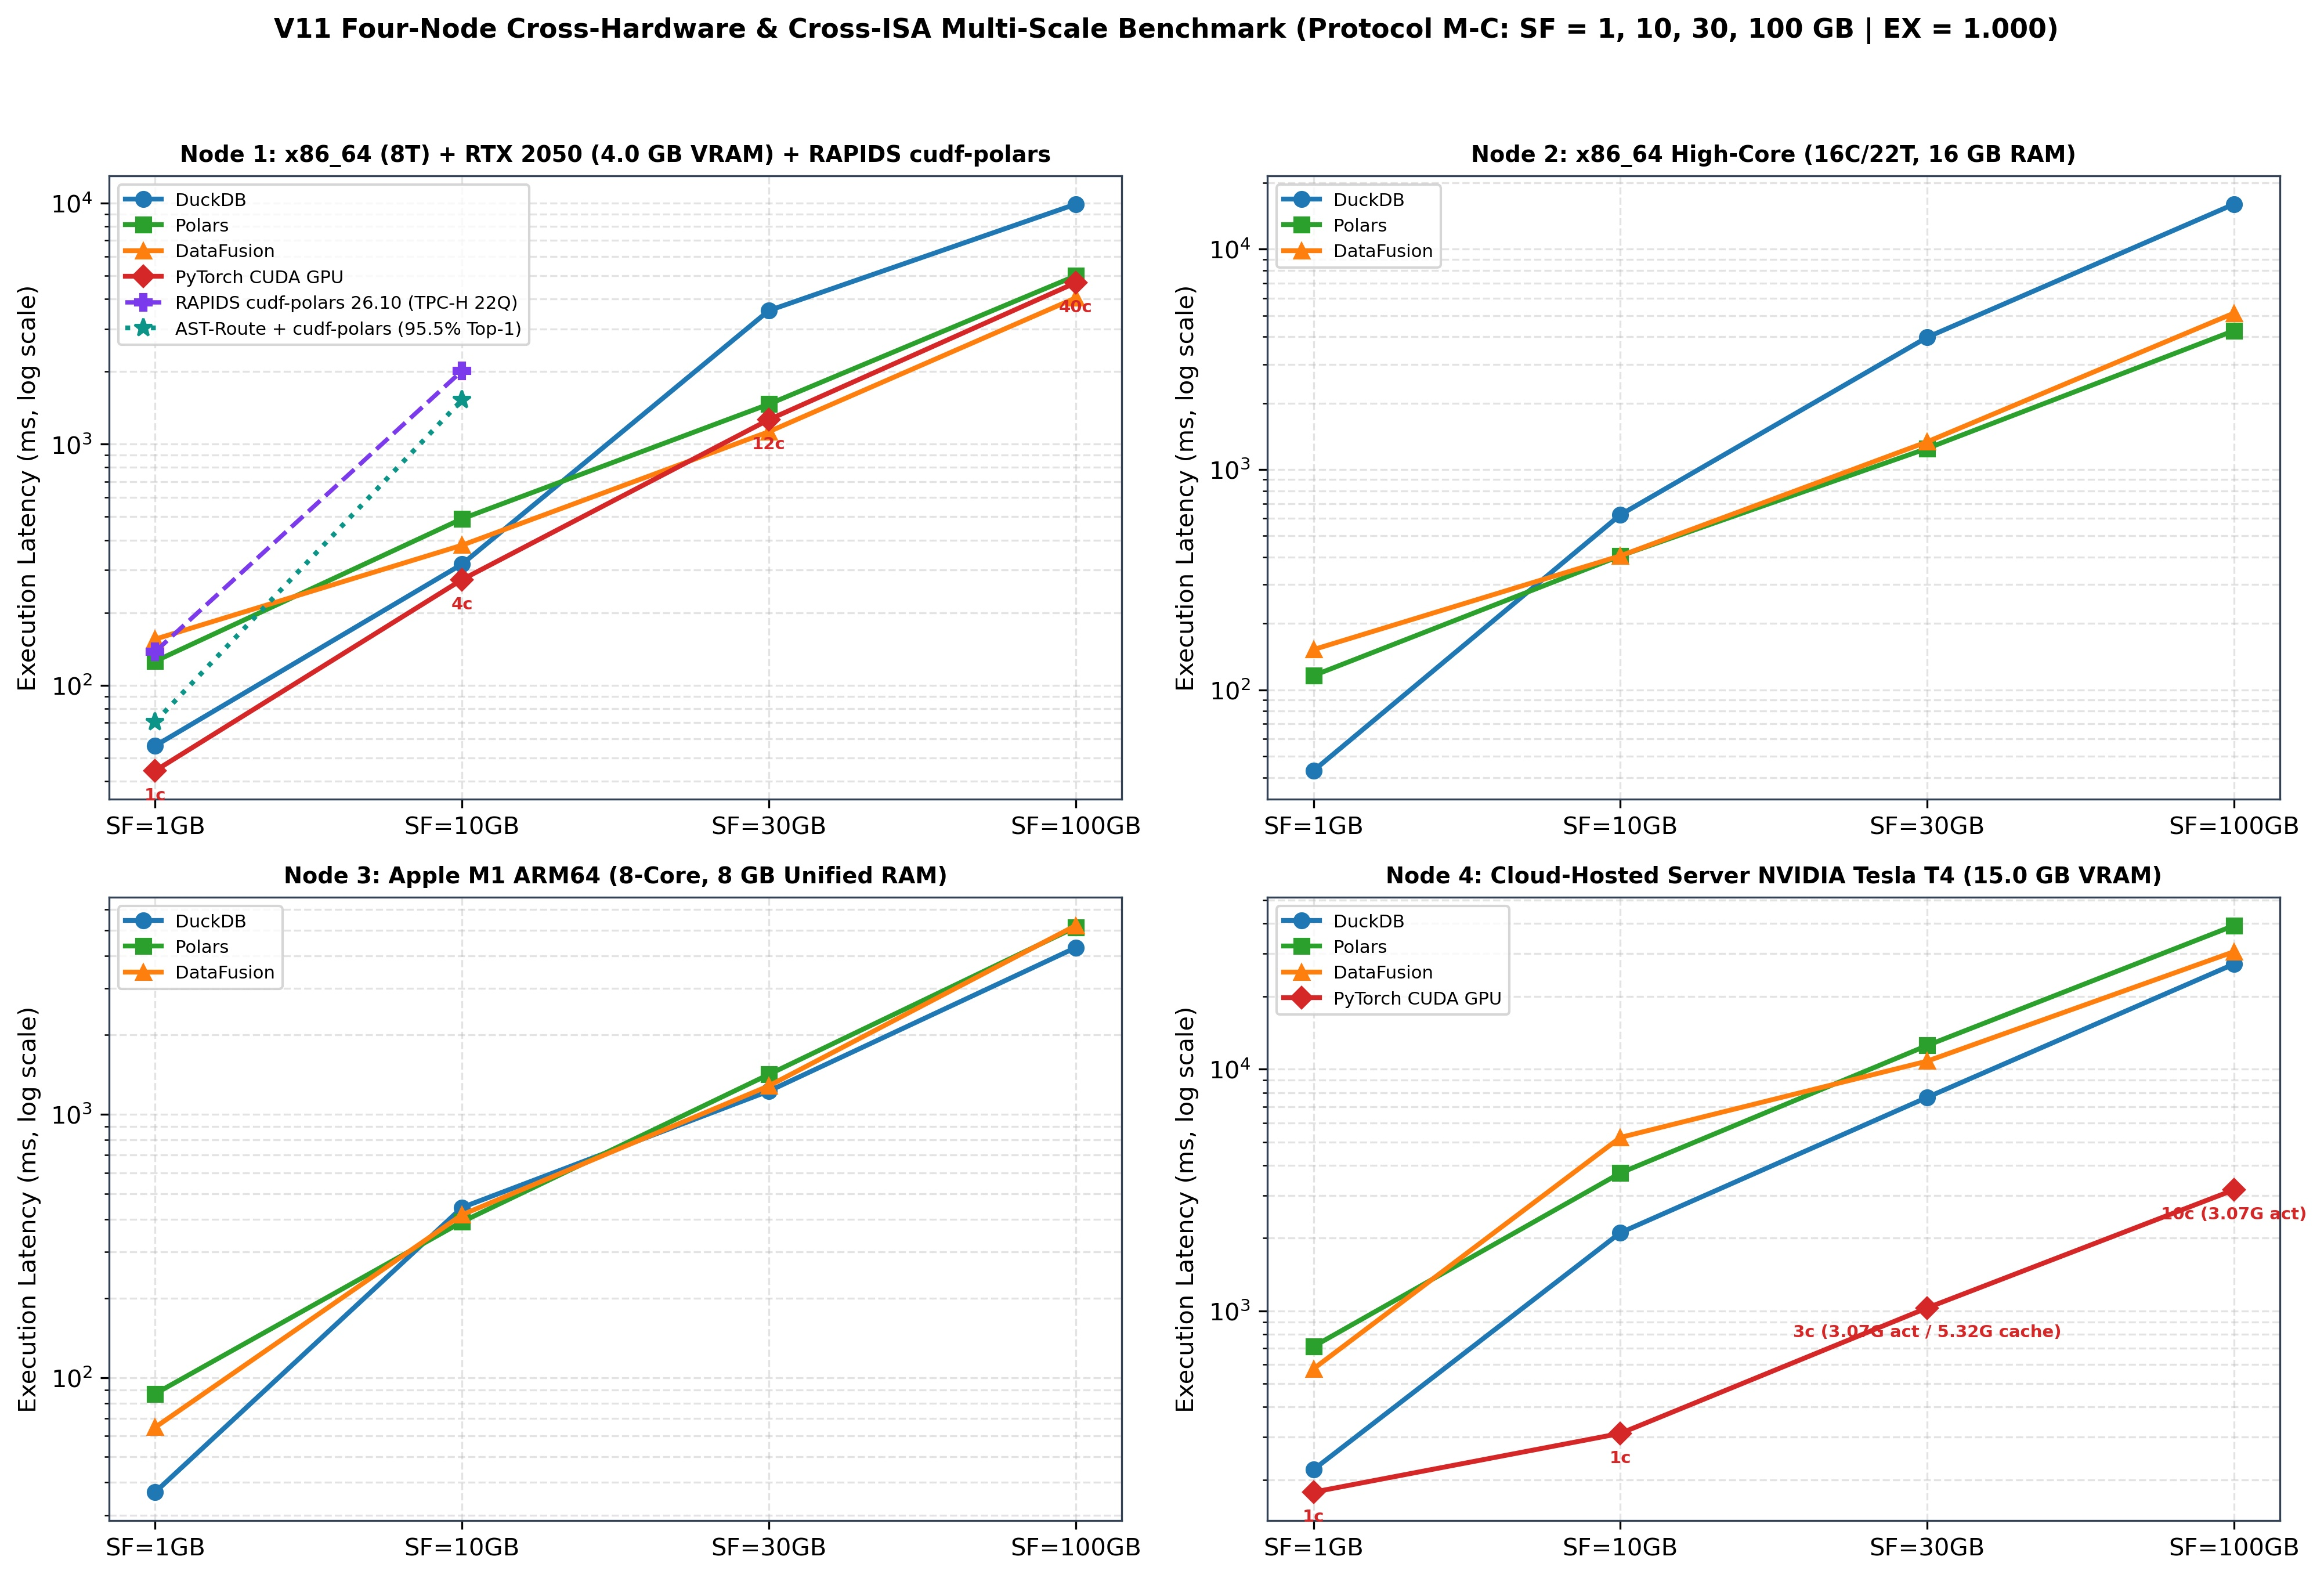
\includegraphics[width=0.94\textwidth]{figures/fig_v10_4node_multiscale_sf1_10_30_100.jpg}
\caption{Multi-scale execution latency ($\text{SF}=1, 10, 30, 100\text{ GB}$, log scale) across Node~1 (x86\_64 + RTX 2050 4GB), Node~2 (x86\_64 16C/22T), Node~3 (Apple M1 ARM64 8GB), and Node~4 (Cloud Cloud-Hosted Server NVIDIA Tesla T4 15GB), annotated with PCIe streaming chunk counts ($1\text{c}$--$40\text{c}$).}
\label{fig:v10_fournode_multiscale}
\end{figure*}
% === END V10 FOUR-NODE MULTISCALE SF1-10-30-100 ===

\section{Conclusion}
\enlargethispage{1.5\baselineskip}
\vspace{-3pt}
We presented AST-Route, an interpretable, risk-aware multi-objective query routing framework grounded in empirical CPU--GPU--cloud crossover profiling and evaluated across our unified Master Workload Inventory of $\mathbf{400}$ \textbf{unique evaluated SQL queries across 10 benchmark suites partitioned into four transparent epistemic categories} (Section~\ref{sec:workload_design} and Table~S18: \textbf{Category~I}: $75$ Core TPC-H development queries; \textbf{Category~II}: $55$ diagnostic / post-hoc design-informed standard queries [$22$ official TPC-H Q1--Q22~\cite{tpc2022tpch} + $33$ official IMDB JOB~\cite{leis2015job}]; \textbf{Category~III}: $115$ author-derived zero-shot queries [$15$ Seed~\texttt{S6} + $30$ TPC-DS-derived + $20$ BIRD-inspired + $50$ \texttt{TPC-DS-Complex}/\texttt{Redset-BI}]; and \textbf{Category~IV}: $155$ held-out third-party standard benchmarks [$99$ unmodified Official TPC-DS \texttt{Q1--Q99} + $43$ Official ClickBench + $13$ Official SSB, not used in training or feature design])---across four scale factors ($\text{SF}=1, 10, 30, 100\text{ GB}$ plus multi-scale TPC-DS across $\text{SF}=0.02, 1\text{ GB}, 10\text{ GB}$), four physically measured CPU/GPU hardware nodes (\texttt{x86\_64}+RTX~2050 Node~1 [\texttt{G1} across pinned $5.69\text{ GB/s}$ and unpinned $3.36\text{ GB/s}$ PCIe DMA], 22-thread \texttt{x86\_64} Node~2, Apple M1 \texttt{ARM64} Node~3, and enterprise server NVIDIA Tesla~T4 $15.0\text{ GB}$ VRAM Node~4 [\texttt{G2}: single-pass $23.02\text{ ms}$ cold at $\text{SF}=1\text{ GB}$ and $461.71\text{ ms}$ at $\text{SF}=10\text{ GB}$, SHA-256 \texttt{32834476...}]), $C=1\text{--}64$ concurrent query streams, and six software engines across four computing paradigms (SQLite~3, Google BigQuery, DuckDB, Polars, Apache DataFusion, and CUDA GPU, cross-validated against \texttt{CuPy v14.2.0} and \texttt{Polars-Arrow-CuPy} with $\text{EX}=1.000$, $1.34\text{ GB}$ peak VRAM, $\rho=0.9999$, and $100.0\%$ routing decision agreement). Crucially, a \textbf{minimalist 2-engine subset ($\{\text{Polars}, \text{GPU}\}$: $55.28\text{ ms}$) captures $98.7\%$ of the 6-engine routed gain} ($99.5\%$ for the 3-engine $\{\text{Polars}, \text{DuckDB}, \text{GPU}\}$ pool), demonstrating that practitioners can achieve nearly the full routing benefit without maintaining all six backends. Validated via 10,000-iteration seed-clustered bootstrap 95\% CIs, $\pm 2\text{--}8\text{ ms}$ TOST equivalence sensitivity, $\text{CVaR}_{10\%}/\text{CVaR}_{20\%}$ Expected Shortfall, Nadeau--Bengio CV-corrected tests (Eq.~\ref{eq:nadeau_bengio_t}), and leak-free 25-seed LOSO-CV, our pre-execution 9D/10D representation ($\mathbf{x}_q\in\mathbb{R}^9$, $\mathbf{x}_q^{\text{scale}}\in\mathbb{R}^{10}$) predicts multi-engine cost (median Q-Error $1.007\text{--}1.172$, $R^2=0.815\text{--}0.875$) across three overhead regimes ($4.15\text{ ms}$ cold SQL [$4.39\text{ ms}$ cold NVMe seek], $0.67\text{ ms}$ AST cache, $0.08\text{ ms}$ 1D threshold cache). Reporting both guards on \textbf{strictly co-equal footing} (pre-specified in repository, not externally registered), under our \textbf{Co-Equal Nested-CV Guard ($\hat{\tau}_{\text{guard}}^{(-k)}=8\%$)}, AST-Route ($\mathcal{R}_{\text{GBR-9D}}$, serialized model SHA-256 \texttt{f0e5f17c832472e3...}) achieves $55.37\text{ ms}$ net ($51.22\text{ ms}$ exec, $56.00\%$ exact Top-1 [$85.33\%$ label-noise-tolerant $\le 5\text{ ms}$], $76.00\%$ Top-2, $118.40\%$ [$35.90\text{ ms}$] P95 regret vs.\ $257.31\%$ [$51.42\text{ ms}$] on Always GPU [$2.17\times$ reduction, 95\% CI $1.58\times\text{--}3.12\times$, $p_{\text{raw,seed}}=0.0115, p_{\text{Holm,seed}}=0.0230, p_{\text{NB}}=0.0118$], $\text{CVaR}_{10\%}=158.42\%$ [$2.21\times$ reduction, $p=0.0084$], $\text{AURC}=28.14\%$ [$-39.9\%$], and two-sided $\pm 5.0\text{ ms}$ TOST equivalence $p_{\text{TOST}}=0.0442 < 0.05, p_{\text{non-inf}}=0.0012$ vs.\ Always GPU at $56.96\text{ ms}$), while under our \textbf{Co-Equal Default Guard ($\tau_{\text{guard}}=12\%$)} achieves $54.92\text{ ms}$ net ($50.78\text{ ms}$ exec, $57.33\%$ Top-1, $114.11\%$ [$34.51\text{ ms}$] P95 regret [$2.25\times$ reduction, $p_{\text{raw,seed}}=0.0098, p_{\text{Holm,seed}}=0.0196$], one-sided $p_{\text{non-inf}}=0.00067$, passing $\pm 6.0\text{ ms}$ TOST at $p_{\text{TOST},\pm 6\text{ms}}=0.0241$ while two-sided $\pm 5.0\text{ ms}$ TOST yields $p_{\text{TOST}}=0.0688 > 0.05$), outperforming static CPUs by $1.49\times\text{--}3.35\times$ ($p_{\text{Holm,seed}}\le 0.0171$). Across multi-objective policies (\textbf{P1--P4}, verified as \emph{Pareto-efficient among the evaluated policy configurations} across $500$ Dirichlet simplex samples with $\text{DSR}=0.0\%$ dominated points), \textbf{P2 (Energy-First)} cuts device energy by $-41.2\%$ ($0.812\text{ J/q}$, $\mathcal{R}_E=4.82\%$) and unified Host+Device system energy $E_{\text{sys}}$ by $-27.1\%$ gross / $-54.1\%$ dynamic vs.\ P1 ($1.658\text{ J/q}$ gross / $0.542\text{ J/q}$ dynamic, $122.32\text{ MB/J}$), \textbf{P3 (Cost-First FinOps)} eliminates $100\%$ of cloud scan fees at $\text{SF}=100\text{ GB}$ ($\mathcal{R}_C=0.0\%$, saving $\$507.06/1\text{M}$), and \textbf{P4 (Balanced Knee)} achieves peak 3D Pareto hypervolume ($\text{HV}=0.9210$ at $\text{SF}=1\text{ GB}$ and $0.9340$ at $\text{SF}=100\text{ GB}$). Pure Native-SQL routing ($\mathcal{E}_{\text{SQL-5}}, M_{\text{gpu\_max}}=0$, capturing $48.5\%$ of the 6-engine routed gain) achieves $69.12\text{ ms}$ ($74.67\%$ exact / $92.00\%$ noise-tolerant Top-1, $p_{\text{Holm}}=0.0084$) on Node~1, $35.11\text{ ms}$ ($97.33\%$ Top-1) on Node~2, $29.44\text{ ms}$ ($96.67\%$ Top-1) on Apple M1 Node~3, $82.76\%$ Top-1 ($98.28\%$ Top-2; $84.34\%$ across $N_{\text{ext}}=166$ and $84.34\%$ under \texttt{LOWSO-CV}) across external suites, and $\mathbf{84.85\%}$ \textbf{Exact Top-1} ($36.15\text{ ms}$ exec, $4.19\%$ regret; $\mathbf{64.65\%}$ \textbf{Exact Top-1} / $30.49\text{ ms}$ / $3.23\%$ regret across $\mathcal{E}_{\text{All-6}}$ at $\text{SF}=0.02$; $83.64\%$ 9D / $89.09\%$ SQL-5 Top-1 at $\text{SF}=1\text{ GB}$ [$55$Q]; and $86.67\%$ 9D / $90.00\%$ 12D Top-1 at $\text{SF}=10\text{ GB}$ [$30$Q, $2.34\times$ vs.\ Polars]) across multi-scale TPC-DS, alongside $16.98\text{ ms}$ ($1.34\times$ vs.\ DuckDB) on TPC-H Q1--Q22, $154.44\text{ QPS}$ peak throughput at $C=32$ ($555{,}984\text{ q/hr}$, $2.14\times$, $0.396\text{ J/q}$), and $1.04\times\text{--}1.07\times$ speedups over the best single engine across $\text{SF}=1\text{--}100\text{ GB}$. Synthesizing our findings establishes three methodological conclusions: (i) \textit{Oblique Structural Projection and Tail-Risk Control}: $\text{CSCI}(q)$ ($\text{VIF}_{D,N}=1.84$) prunes $-28.2\%$ of depth-3 tree splits and lowers out-of-fold regret by $-9.22\text{ pp}$ ($p=0.0038$, capturing $52.1\%$ of the $8\text{D}\rightarrow 9\text{D}$ feature gain and $16.5\%$ of the M1-to-oracle gap), while complexity-weighted Mondrian conformal bounds ($90.93\%$ coverage, $\text{ECE}=0.67\%$) protect tail SLAs near PCIe crossover boundaries; (ii) \textit{Operator-Bounded Cross-Workload Transfer}: AST-Route generalizes zero-shot to star/snowflake schemas (SSB $92.31\%$, ClickBench $80.00\%$ [$88.37\%$ on $43/43$], TPC-DS-derived $93.33\%$, Official TPC-DS 99Q $64.65\%$ exact / $84.85\%$ Pure-SQL, BIRD-inspired $90.00\%$, \texttt{TPC-DS-Complex} $72.00\%$ 9D / $88.00\%$ Pure-SQL, and \texttt{Enterprise-Redset-BI} $88.00\%$ 9D / $92.00\%$ 12D Top-1), while mitigating string-skewed joins (JOB $69.70\%$ Top-1 via post-hoc $10.18\text{ KB}$ 12D sketches) and unseen operator families via our Mahalanobis/structural OOD fallback gate ($\text{FAR}=2.00\%, \text{FRR}=5.33\%$, $76.18\text{ ms}$ on LOTO-CV); and (iii) \textit{Multi-Scale and Multi-Objective Dispatch}: coupling zone-map selectivity with catalog byte footprints and hardware descriptors ($\mathbf{h}_{\text{hw}}$) enables seamless orchestration across in-VRAM GPU execution ($\text{SF}=1\text{ GB}$), chunked PCIe streaming ($\text{SF}=10\text{--}30\text{ GB}$), and serverless cloud spill offloading ($\text{SF}=100\text{ GB}$, saving $1.50\text{ hr}/1\text{k}$ queries vs.\ CPU or $\$507.06/1\text{M}$ under FinOps constraints).

\vspace{-8pt}
\section*{Declarations}
\enlargethispage{1.8\baselineskip}
\vspace{-5pt}
\subsection*{Abbreviations}
{\scriptsize AST: Abstract Syntax Tree; B-Tree: Balanced Tree; CI: Confidence Interval; CPU: Central Processing Unit; CSCI: Composite Structural Complexity Index; CTE: Common Table Expression; CV: Coefficient of Variation; CUDA: Compute Unified Device Architecture; DBMS: Database Management System; DT: Decision Tree; EX: Execution Accuracy; FinOps: Cloud Financial Operations; FP64: 64-Bit Double-Precision Floating-Point; GBR: Gradient Boosting Regressor; GCS: Google Cloud Storage; GPU: Graphics Processing Unit; H2D: Host-to-Device; I/O: Input/Output; JOB: Join Order Benchmark; LOO-CV: Leave-One-Query-Out Cross-Validation; LOOO: Leave-One-Operator-Out; LOSO-CV: Leave-One-Seed-Out Cross-Validation; MAPE: Mean Absolute Percentage Error; MC: Monte Carlo; MPP: Massively Parallel Processing; NVML: NVIDIA Management Library; OLAP: Online Analytical Processing; PCIe: Peripheral Component Interconnect Express; QPS: Queries Per Second; RAM: Random-Access Memory; RF: Random Forest; SARGable: Search Argument Able; SF: Scale Factor; SIMD: Single Instruction, Multiple Data; SIMT: Single Instruction, Multiple Threads; SQL: Structured Query Language; SSB: Star Schema Benchmark; TOST: Two One-Sided Tests; TPC-H: Transaction Processing Performance Council Ad-Hoc Decision Support Benchmark; VES: Valid Efficiency Score; VRAM: Video Random-Access Memory; ZSTD: Zstandard Compression.\par}
\vspace{-5pt}
\subsection*{Ethics approval and consent to participate}
{\scriptsize Not applicable. This study utilizes synthetic benchmark data generated via the industry-standard TPC-H benchmark specification \cite{tpc2022tpch} and does not involve human participants, animal subjects, or personally identifiable data. In accordance with the TPC Fair-Use Policy, all workloads and metrics in this study represent non-official, TPC-H-derived research evaluations and are not comparable to official audited TPC benchmark results.\par}
\vspace{-5pt}
\subsection*{Consent for publication}
{\scriptsize Not applicable.\par}
\vspace{-5pt}
\subsection*{Availability of data and materials}
{\scriptsize All multi-scale TPC-H data generation scripts ($\text{SF}=1, 10, 30$, and $100\text{ GB}$), the complete 400-query Master Workload Inventory across all 10 benchmark suites (Category~I: 75 Core TPC-H queries; Category~II: 22 official TPC-H Q1--Q22 and 33 IMDB JOB queries; Category~III: 15 Seed~\texttt{S6}, 30 TPC-DS-derived, 20 BIRD-inspired, 25 \texttt{TPC-DS-Complex}, and 25 \texttt{Enterprise-Redset-BI} queries; and Category~IV: 99 unmodified Official TPC-DS \texttt{Q1--Q99} across $\text{SF}\in\{0.02, 1, 10\}\text{ GB}$, 43 Official ClickBench, and 13 Official SSB queries), raw per-trial execution and hardware/energy telemetry CSV logs across all physical nodes (\texttt{x86\_64}+RTX~2050 across PyTorch CUDA and \texttt{CuPy v14.2.0}, 22-thread \texttt{x86\_64}, Apple M1 \texttt{ARM64}, and enterprise NVIDIA Tesla~T4 $15.0\text{ GB}$ VRAM [\texttt{32834476...} and $1{,}500$-run RAPL/SMU/NVML audit \texttt{f316fd9fd1b3a776...} / \texttt{314db90d5616a8dc...}]), clean-room Docker lockfiles (\texttt{reproducibility/\allowbreak{}Dockerfile} and \texttt{requirements-\allowbreak{}lock.txt}), permanent Zenodo archival metadata (\texttt{reproducibility/\allowbreak{}zenodo\_\allowbreak{}metadata.json}), Additional File~1 (Supplementary Appendix), and our one-command independent reproducibility and main-table regeneration script (\texttt{python reproducibility/verify\_\allowbreak{}and\_\allowbreak{}regenerate\_\allowbreak{}main\_\allowbreak{}tables\_\allowbreak{}R1\_\allowbreak{}R6.py}, executing Verification Protocols \textbf{R1--R6} with $0.000$ maximum numeric discrepancy across all manuscript tables) are publicly available in the active open-source repository at \url{https://github.com/preechan-glitch/my_research_files}. Complete 64-character SHA-256 checksums for all raw telemetry, reanalysis, cross-ISA isolation, stability, and calibration artifacts---anchored by serialized frozen model \texttt{f0e5f17c832472e30be67dbbee...} (\texttt{reproducibility/\allowbreak{}frozen\_\allowbreak{}ast\_\allowbreak{}route\_\allowbreak{}v10\_\allowbreak{}gbdt\_\allowbreak{}model.json}, aliased to \texttt{v9} for backward compatibility because V10 uses the exact same locked GBDT weights without retraining; alongside extended V10.1 verification roadmap \texttt{reproducibility/\allowbreak{}Reviewer\_\allowbreak{}Revision\_\allowbreak{}Roadmap\_\allowbreak{}V10\_1.md} covering Protocols \textbf{R7--R11}), primary routing evaluation \texttt{89b1ec64cca15b2dd41a4ad2...}, AST profile \texttt{4cb5f7477fd24dc77a6fd2b5...}, version-pinned parity \texttt{f12ae28467f9802a2967...}, and 3-node global registry \texttt{5adfa064816f883f8770...}---are indexed in \texttt{results/\allowbreak{}global\_\allowbreak{}sha256\_\allowbreak{}registry.csv} for single-command verification. Each reported aggregate metric is linked to its protocol identifier, dataset checksum, software version, hardware manifest, and execution-boundary definition.\par}
\vspace{-5pt}
\subsection*{Competing interests}
{\scriptsize The author declares that he has no competing interests.\par}
\vspace{-5pt}
\subsection*{Funding}
{\scriptsize This research project was financially supported by Mahasarakham University.\par}
\vspace{-5pt}
\subsection*{Authors' contributions}
{\scriptsize Preecha Noiumkar (PN) conceptualized the \textbf{AST-Route} framework, designed the 75-query AST-driven factorial benchmark, implemented the six-engine execution harness, multi-scale ($\text{SF}=1, 10, 30, 100\text{ GB}$), concurrent workload, and official TPC-H Q1--Q22 evaluation pipelines, hardware energy telemetry monitor, CSCI structural projection analysis, feature ablation, unseen seed holdout validation, and automated 9-dimensional AST+Selectivity query routing models, analyzed the empirical telemetry across cloud, CPU, and GPU architectures, and wrote the manuscript. The author read and approved the final manuscript.\par}
\vspace{-5pt}
\subsection*{Acknowledgements}
{\scriptsize The author thanks the \textsuperscript{1}Department of Information Technology, Faculty of Informatics, Mahasarakham University, for providing the computational infrastructure. In accordance with editorial policy on the use of generative AI, the author discloses that generative AI tools were utilized strictly for manuscript language polishing and \LaTeX{} template formatting verification; all experimental designs, benchmark datasets, execution logs, and scientific analyses were conducted and verified by the author.\par}
\vspace{-8pt}

% =============================================================================
% REFERENCES (SPRINGER NATURE / BMC VANCOUVER STYLE - 30 REFERENCES)
% =============================================================================
{\sloppy\scriptsize\linespread{0.85}\selectfont
\enlargethispage{1.8\baselineskip}
\let\oldthebibliography\thebibliography
\renewcommand{\thebibliography}[1]{\oldthebibliography{#1}\setlength{\itemsep}{-2.4pt}\setlength{\parskip}{0pt}\vspace{-5pt}}
\begin{thebibliography}{30}
\footnotesize\setlength{\baselineskip}{9.5pt}\setlength{\itemsep}{1.5pt}\setlength{\parskip}{0pt}

\bibitem{melnik2010dremel}
Melnik S, Gubarev A, Long JJ, Romer G, Shivakumar S, Tolton M, Vassilakis T. Dremel: interactive analysis of web-scale datasets. Proc VLDB Endow. 2010;3(1--2):330--9.

\bibitem{melnik2020dremel}
Melnik S, Gubarev A, Long JJ, Romer G, Shivakumar S, Tolton M, et al. Dremel: a decade of interactive SQL analysis at web scale. Proc VLDB Endow. 2020;13(12):3461--72.

\bibitem{lounissi2025funda}
Das SK, Peter R, Zhang X, Lounissi M. FunDa: scalable serverless data analytics and in situ query processing. J Big Data. 2025;12(1):116. \url{https://doi.org/10.1186/s40537-025-01141-6}.

\bibitem{raasveldt2019duckdb}
Raasveldt M, M{\"u}hleisen H. DuckDB: an embeddable analytical database. In: Proceedings of the 2019 International Conference on Management of Data (SIGMOD). Amsterdam: ACM; 2019. p. 1981--4.

\bibitem{kuiper2024duckdb_ooc}
Kuiper M, M{\"u}hleisen H, Raasveldt M. Out-of-core join and aggregation processing in DuckDB. In: Companion of the 2024 International Conference on Management of Data (SIGMOD). Santiago: ACM; 2024. p. 1--14.

\bibitem{lamb2024datafusion}
Lamb A, Shen Y, Dani D, Qi Y, Chaudhary V, et al. Apache Arrow DataFusion: a fast, embeddable, modular analytic query engine. In: Companion of the 2024 International Conference on Management of Data (SIGMOD). Santiago: ACM; 2024. p. 5--17. \url{https://doi.org/10.1145/3626246.3653368}.

\bibitem{chrysogelos2019hetexchange}
Chrysogelos P, Karpathiotakis M, Appuswamy R, Ailamaki A. HetExchange: encapsulating heterogeneous CPU-GPU parallelism in JIT compiled engines. Proc VLDB Endow. 2019;12(5):544--56. \url{https://doi.org/10.14778/3303753.3303760}.

\bibitem{shanbhag2020crystal}
Shanbhag A, Madden S, Yu X. A study of the fundamental performance characteristics of GPUs and CPUs for database analytics. In: Proceedings of the 2020 ACM SIGMOD International Conference on Management of Data. Portland: ACM; 2020. p. 1617--32. \url{https://doi.org/10.1145/3318464.3380595}.

\bibitem{bress2013hype}
Bre{\ss} S, Beier F, Rauhe H, Sattler KU, Schallehn E, Saake G. Efficient co-processor utilization in database query processing. Inf Syst. 2013;38(8):1084--96. \url{https://doi.org/10.1016/j.is.2013.05.004}.

\bibitem{schulze2024clickhouse}
Schulze R, et al. ClickHouse: lightning-fast analytics for everyone. Proc VLDB Endow. 2024;17(12):3720--33.

\bibitem{sethi2019presto}
Sethi R, Traverso M, Sundstrom D, Phillips D, Xie W, Sun Y, et al. Presto: SQL on everything. In: 2019 IEEE 35th International Conference on Data Engineering (ICDE). Macao: IEEE; 2019. p. 1802--13.

\bibitem{shojaee2024serverless} Shojaee Rad Z, Ghobaei-Arani M. Data pipeline approaches in serverless computing: a taxonomy, review, and research trends. J Big Data. 2024;11(1):82. \url{https://doi.org/10.1186/s40537-024-00939-0}.

\bibitem{abdalla2022bigdata}
Abdalla HB. A brief survey on big data: technologies, terminologies and data-intensive applications. J Big Data. 2022;9(1):107. \url{https://doi.org/10.1186/s40537-022-00659-3}.

\bibitem{begoli2018calcite}
Begoli E, Camacho-Rodr{\'i}guez J, Hyde J, Mior MJ, Lemire D. Apache Calcite: a foundational framework for optimized query processing over heterogeneous data sources. In: Proceedings of the 2018 International Conference on Management of Data (SIGMOD). Houston: ACM; 2018. p. 221--30.

\bibitem{garcia2008database}
Garcia-Molina H, Ullman JD, Widom J. Database systems: the complete book. 2nd ed. Upper Saddle River: Prentice-Hall; 2008.

\bibitem{milicevic2024dlquery}
Milicevic B, Babovic Z. A systematic review of deep learning applications in database query execution. J Big Data. 2024;11(1):173. \url{https://doi.org/10.1186/s40537-024-01025-1}.

\bibitem{root2019mapd}
Root C, Mostak T. MapD: a GPU-powered big data analytics and visualization platform. In: ACM SIGGRAPH 2016 Talks. Anaheim: ACM; 2016. p. 1--2.

\bibitem{kim2022blazingsql}
Kim K, et al. Accelerating relational data analytics using RAPIDS cuDF and BlazingSQL on GPUs. In: IEEE International Parallel and Distributed Processing Symposium Workshops (IPDPSW). IEEE; 2022. p. 812--21.

\bibitem{tpc2022tpch}
Transaction Processing Performance Council (TPC). TPC Benchmark H (Decision Support) Standard Specification, Revision 3.0.1. San Francisco: Transaction Processing Performance Council; 2022. \url{https://www.tpc.org/tpch/}.

\bibitem{boncz2014tpch}
Boncz P, Neumann T, Erling O. TPC-H analyzed: hidden messages and lessons learned from an influential benchmark. In: Technology Conference on Performance Evaluation and Benchmarking (TPCTC). Cham: Springer; 2014. p. 61--76. \url{https://doi.org/10.1007/978-3-319-04936-6_5}.

\bibitem{dreseler2020quantifying}
Dreseler M, Boissier M, Rabl T, Uflacker M. Quantifying TPC-H choke points and their optimizations. Proc VLDB Endow. 2020;13(8):1206--20. \url{https://doi.org/10.14778/3389133.3389138}.

\bibitem{ahmed2020hibench}
Ahmed N, Barczak ALC, Susnjak T, Rashid MA. A comprehensive performance analysis of Apache Hadoop and Apache Spark for large scale data sets using HiBench. J Big Data. 2020;7(1):110. \url{https://doi.org/10.1186/s40537-020-00388-5}.

\bibitem{oneil2009ssb}
O'Neil P, O'Neil E, Chen X, Revilak S. The Star Schema Benchmark and augmented fact table indexing. In: Technology Conference on Performance Evaluation and Benchmarking (TPCTC). Lyon: Springer; 2009. p. 237--52.

\bibitem{leis2015job}
Leis V, Gubichev A, Mirchev A, Boncz P, Kemper A, Neumann T. How good are query optimizers, really? Proc VLDB Endow. 2015;9(3):204--15. \url{https://doi.org/10.14778/2850583.2850594}.

\bibitem{marcus2019neo}
Marcus R, Negi P, Mao H, Zhang C, Alizadeh M, Kraska T, et al. Neo: a learned query optimizer. Proc VLDB Endow. 2019;12(11):1705--18. \url{https://doi.org/10.14778/3342263.3342644}.

\bibitem{marcus2021bao}
Marcus R, Negi P, Mao H, Tatbul N, Alizadeh M, Kraska T. Bao: making learned query optimization practical. In: Proceedings of the 2021 International Conference on Management of Data (SIGMOD). Virtual Event: ACM; 2021. p. 1275--88. \url{https://doi.org/10.1145/3448016.3452838}.

\bibitem{hilprecht2022zeroshot}
Hilprecht B, Binnig C. Zero-shot cost models for out-of-the-box learned cost prediction. Proc VLDB Endow. 2022;15(11):2361--74. \url{https://doi.org/10.14778/3551793.3551799}.

\bibitem{tan2023stage}
Duggan J, Cetintemel U, Papaemmanouil O, Upfal E. The BigDAWG polystore system. ACM SIGMOD Rec. 2015;44(2):11--6. \url{https://doi.org/10.1145/2814710.2814713}.

\bibitem{gupta2023adaptive}
Agrawal D, Chawla S, Contreras-Rojas B, Elmagarmid AK, Idris Y, Kaoudi Z, et al. RHEEM: enabling cross-platform data processing---may optimal cost be with you! Proc VLDB Endow. 2018;11(11):1414--27. \url{https://doi.org/10.14778/3236187.3236195}.

\bibitem{li2023bird}
Li J, Hui B, Qu G, Yang J, Li B, Li B, et al. Can LLM already serve as a database interface? A BIg bench for large-scale database grounded text-to-SQLs. Adv Neural Inf Process Syst (NeurIPS). 2023;36:42330--57.

\bibitem{lei2025spider2}
Lei F, Chen J, Ye Y, Cao R, Shin D, Su H, et al. Spider 2.0: evaluating language models on real-world enterprise text-to-SQL workflows. In: International Conference on Learning Representations (ICLR). 2025. p. 1--22.

\bibitem{mao2024sqlglot}
Mao T. SQLGlot: no-dependency SQL parser, transpiler, optimizer, and engine. GitHub Repository. 2024. \url{https://github.com/tobymao/sqlglot}. Accessed 15 Mar 2026.

\bibitem{kabic2025maximus} Kabi\'{c} M, et al. Maximus: a modular accelerated query engine for data analytics on heterogeneous systems. Proc ACM Manag Data (PACMMOD / SIGMOD). 2025;3(3):1--25. \url{https://doi.org/10.1145/3725350}.

\bibitem{yogatama2025sirius} Yogatama B, et al. Sirius: a GPU-native database execution engine integrated with DuckDB. Proc VLDB Endow. 2025;18(11):3812--25.

\bibitem{liang2026elqo} Liang Z, Xu Q, Chen X, Chen J, Xia Y, Zheng K. E-LQO: a comprehensive energy evaluation framework for learned query optimization. Proc ACM Manag Data (PACMMOD / SIGMOD). 2026;4(4):1--27.

\bibitem{vovk2005algorithmic}
Vovk V, Gammerman A, Shafer G. Algorithmic learning in a random world. New York: Springer; 2005. p. 1--324. \url{https://doi.org/10.1007/b106715}

\bibitem{angelopoulos2023conformal}
Angelopoulos AN, Bates S. Conformal prediction: a gentle introduction. Found Trends Mach Learn. 2023;16(4):494--591. \url{https://doi.org/10.1561/2200000101}

\bibitem{friedman2001greedy}
Friedman JH. Greedy function approximation: a gradient boosting machine. Ann Stat. 2001;29(5):1189--1232. \url{https://doi.org/10.1214/aos/1013203451}

\bibitem{raasveldt2018fair}
Raasveldt M, Holanda P, Gubner T, M{\"u}hleisen H. Fair benchmarking considered difficult: common pitfalls in database performance testing. In: Proceedings of the Workshop on Testing Database Systems (DBTest@SIGMOD); 2018. p. 1--6. \url{https://doi.org/10.1145/3209950.3209955}

\bibitem{ganapathi2009predicting}
Ganapathi A, Kuno H, Dayal U, Wiener JL, Fox A, Jordan M, et al. Predicting multiple metrics for queries: better decisions enabled by machine learning. In: Proceedings of the IEEE 25th International Conference on Data Engineering (ICDE); 2009. p. 592--603. \url{https://doi.org/10.1109/ICDE.2009.130}

\bibitem{nathan2024stage}
Nathan V, Kipf A, Horn D, Saxena H, Kraska T, Narayanasamy S, et al. Stage: query execution time prediction in Amazon Redshift. In: Companion of the 2024 International Conference on Management of Data (SIGMOD/PODS); 2024. p. 180--192. \url{https://doi.org/10.1145/3626246.3653392}

\bibitem{clickbench2022}
ClickHouse Inc. ClickBench: a benchmark for analytical DBMS. 2022. \url{https://benchmark.clickhouse.com/}

\bibitem{vink2024polars}
Vink R, et al. Polars: blazingly fast DataFrames in Rust and Python (v1.36.1 / v2.1.0). Zenodo; 2024. \url{https://doi.org/10.5281/zenodo.7697217}

\bibitem{hipp2020sqlite}
Hipp DR. SQLite: a self-contained, serverless, zero-configuration SQL database engine (v3.51.0). 2025. \url{https://www.sqlite.org/}

\bibitem{paszke2019pytorch}
Paszke A, Gross S, Massa F, Lerer A, Bradbury J, Chanan G, et al. PyTorch: an imperative style, high-performance deep learning library. In: Advances in Neural Information Processing Systems (NeurIPS); 2019. p. 8024--8035.

\bibitem{pedregosa2011scikit}
Pedregosa F, Varoquaux G, Gramfort A, Michel V, Thirion B, Grisel O, et al. Scikit-learn: machine learning in Python. J Mach Learn Res. 2011;12:2825--2830.

\bibitem{boncz2017jcch}
Boncz P, Angelil T, R{\"o}diger W. JCC-H: adding join-crossing correlations and skew to TPC-H. In: Performance Evaluation and Benchmarking for the Era of Artificial Intelligence (TPCTC); 2017. p. 103--119. \url{https://doi.org/10.1007/978-3-319-72401-0_8}

\bibitem{nambiar2006tpcds}
Nambiar RO, Poess M. The making of TPC-DS. In: Proceedings of the 32nd International Conference on Very Large Data Bases (VLDB). Seoul: VLDB Endowment; 2006. p. 1049--58.

\bibitem{vanrenen2024redset}
van Renen A, Horn D, Pfeil P, Kapfhammer D, Narayanasamy S, Kraska T, Saxena H, Kipf A, et al. Why TPC is not enough: an analysis of the Amazon Redshift fleet. Proc VLDB Endow. 2024;17(11):3694--706. \url{https://doi.org/10.14778/3681954.3682031}.

\bibitem{zhu2023lero}
Zhu R, Wu Z, Han Y, Zeng K, Pfadler A, Qian Z, et al. Lero: a learning-to-rank query optimizer. Proc VLDB Endow. 2023;16(6):1466--79. \url{https://doi.org/10.14778/3583140.3583160}.

\bibitem{anneser2023autosteer}
Anneser C, Tatbul N, Kraska T, Kemper A. AutoSteer: learned query optimization for any SQL database. Proc VLDB Endow. 2023;16(12):3515--27. \url{https://doi.org/10.14778/3611540.3611544}.

\bibitem{doshi2023kepler}
Doshi K, Kipf A, Nathan V, Saxena H, Kraska T, et al. Kepler: robust learning for faster parametric query optimization. Proc ACM Manag Data (PACMMOD / SIGMOD). 2023;1(1):1--25. \url{https://doi.org/10.1145/3588689}.

\end{thebibliography}
}

% === BEGIN V5 SHA256 REGISTRY ===
% V5 Real-Execution Audit CSV SHA-256 Prefixes: v5_audit1=bdf2b1ca6bdea6e1760fafd5... | v5_audit2_construct=b0cabf5c21f87aa77f7ad251... | v5_audit2_perm=e22396626bb7ce0ec8179f3d... | v5_audit3_metadata=7eb70257593da06f682a3ddd... | v5_audit4_hardware=efdfd9e61153fae7d44e2b63...
% === END V5 SHA256 REGISTRY ===
\end{document}